\documentclass{article}

\usepackage{amsmath,geometry,amsfonts,array,makecell,enumitem,bm,esint,booktabs,multirow,mathtools,upgreek,amssymb,pgfplots,mathrsfs,nicematrix}
\usepackage[amsmath]{ntheorem}
\usepackage[hidelinks]{hyperref}
\usepackage[nameinlink,noabbrev]{cleveref}
\usepackage[thinlines]{easytable}
\usepackage{fancyhdr}
\pagestyle{fancy}
\fancyhead[L]{\itshape\nouppercase{\leftmark}}
\fancyhead[R]{II Principles of Quantum Mechanics}

\title{Principles of Quantum Mechanics}
\author{Yue Wu}

\geometry{a4paper,hmargin=1.1in,vmargin=1.2in}

\setlength{\parskip}{1em}
\tolerance=1000
\emergencystretch=1em
\hyphenpenalty=1000
\exhyphenpenalty=100
\righthyphenmin=3

\pgfplotsset{compat=1.18}
\usetikzlibrary{decorations.markings}

\theoremstyle{plain}\theoremheaderfont{\normalfont\itshape}\theorembodyfont{\rmfamily}\theoremseparator{.}\newtheorem*{rem}{Remark}\newtheorem*{ex}{Example}\newtheorem*{proof}{Proof}\newtheorem*{altp}{Alternative proof}

\theoremstyle{plain}\theoremheaderfont{\normalfont\bfseries}\theorembodyfont{\rmfamily}\theoremseparator{.}\newtheorem{thm}{Theorem}[section]\newtheorem{lem}[thm]{Lemma}\newtheorem{prop}[thm]{Proposition}\newtheorem*{cor}{Corollary}\newtheorem{defn}[thm]{Definition}\newtheorem{clm}[thm]{Claim}\newtheorem{clminproof}{Claim}

\theoremstyle{break}\theoremheaderfont{\normalfont\itshape}\theorembodyfont{\rmfamily}\theoremseparator{.\medskip}\newtheorem*{proofskip}{Proof}\newtheorem*{exs}{Examples}\newtheorem*{rems}{Remarks}

\theoremstyle{break}\theoremheaderfont{\normalfont\bfseries}\theorembodyfont{\rmfamily}\theoremseparator{.\medskip}\newtheorem{lemskip}[thm]{Lemma}\newtheorem{defnskip}[thm]{Definition}\newtheorem{propskip}[thm]{Proposition}\newtheorem{thmskip}[thm]{Theorem}

\crefname{thm}{Theorem}{Theorems}\crefname{defn}{Definition}{Definitions}\crefname{lem}{Lemma}{Lemmas}\crefname{lemskip}{Lemma}{Lemmas}\crefname{cor}{Corollary}{Corollaries} \crefname{prop}{Proposition}{Propositions}\crefname{clm}{Claim}{Claims}

\setcounter{tocdepth}{2}
\setcounter{section}{0}
\numberwithin{equation}{section}

\newcommand{\qed}{\hfill\ensuremath{\Box}}
\newcommand{\unit}[1]{\ \mathrm{#1}}
\newcommand{\ii}{\mathrm{i}}
\newcommand{\ee}{\mathrm{e}}
\newcommand{\tp}{^\mathrm{T}}
\newcommand{\dd}[2][]{\mathrm{d}^{#1} #2\,}
\renewcommand{\d}[2][]{\mathrm{d}^{#1} #2}
\newcommand{\dv}[3][]{\frac{\mathrm{d}^{#1} #2}{{\mathrm{d} #3}^{#1}}}
\newcommand{\pdv}[3][]{\frac{\partial^{#1} #2}{{\partial #3}^{#1}}}
\newcommand{\bra}[1]{\left\langle #1 \right|}
\newcommand{\ket}[1]{\left| #1 \right\rangle}
\newcommand{\braket}[2]{\left\langle #1 \middle| #2 \right\rangle}
\newcommand{\mel}[3]{\left\langle #1 \middle| #2 \middle| #3 \right\rangle}
\newcommand{\redmel}[3]{\left\langle #1 \middle\| #2 \middle\| #3 \right\rangle}
\newcommand{\eval}[1]{\left\langle #1 \right\rangle}
\newcommand{\expval}[2]{\left\langle #2 \middle| #1 \middle| #2 \right\rangle}
\newcommand{\vb}[1]{\bm{\mathrm{#1}}}
\newcommand{\vu}[1]{\hat{\bm{\mathrm{#1}}}}
\newcommand{\cross}{\bm{\times}}
\newcommand{\vdot}{\bm{\cdot}}
\newcommand{\abs}[1]{\left| #1 \right|}
\newcommand{\norm}[1]{\left\| #1 \right\|}
\newcommand{\grad}{\vb{\nabla}}
\renewcommand{\div}{\vb{\nabla}\cdot}
\newcommand{\curl}{\vb{\nabla}\times}
\newcommand{\laplacian}{\nabla^2}
\newcommand{\hb}{\mathcal{H}}
\newcommand{\ph}{\mathbb{P}\mathcal{H}}
\DeclareMathOperator{\Id}{Id}
\DeclareMathOperator{\Prob}{Prob}
\DeclareMathOperator{\sech}{sech}
\DeclareMathOperator{\Dom}{Dom}
\DeclareMathOperator{\tr}{tr}
\DeclareMathOperator{\diag}{diag}
\DeclareMathOperator{\Sym}{Sym}
\DeclareMathOperator{\spn}{span}
\renewcommand{\Re}{\operatorname{Re}}
\renewcommand{\Im}{\operatorname{Im}}
\newcommand{\NN}{\mathbb{N}}
\newcommand{\ZZ}{\mathbb{Z}}
\newcommand{\QQ}{\mathbb{Q}}
\newcommand{\RR}{\mathbb{R}}
\newcommand{\CC}{\mathbb{C}}
\newcommand{\SO}{\mathrm{SO}}
\newcommand{\E}{\mathrm{E}}
\newcommand{\U}{\mathrm{U}}
\newcommand{\SU}{\mathrm{SU}}
\renewcommand{\S}{_{\mathrm{S}}}
\newcommand{\I}{_{\mathrm{I}}}
\DeclareMathOperator{\Texp}{T\, exp}


\NiceMatrixOptions{cell-space-limits = 2pt}


\begin{document}
    \setlength{\parindent}{0pt}
	\Huge\textsf{\textbf{Principles of Quantum Mechanics}}
		
	\Large\textsf{\textbf{University of Cambridge Part II Mathematical Tripos}}

	\noindent\makebox[\linewidth]{\rule{\textwidth}{2pt}}

	\large\textsf{\textbf{Yue Wu}}
	\begin{itemize}[topsep=0pt,leftmargin=15pt]
		\item[] \textit{Yusuf Hamied Department of Chemistry\\
		Lensfield Road,\\
		Cambridge, CB2 1EW}\\

		\textit{yw628@cam.ac.uk}
	\end{itemize}
    \thispagestyle{empty}
    \pagenumbering{roman}
    \setlength{\parindent}{15pt}

    \newpage
    \begin{center}
		\textbf{\Large{Acknowledgements}}
	\end{center}
	\large
	Nothing in these lecture notes is original. They are largely based on the notes by Prof. David Skinner, who lectured this course in 2021, and his notes can be found \textcolor{blue}{\href{https://www.damtp.cam.ac.uk/user/dbs26/PQM.html}{here}}. Moreover, they are nowhere near accurate representations of what was actually lectured, and in particular, all errors are almost surely mine.

    \normalsize
	\newpage
	\tableofcontents
	\newpage
    \pagenumbering{arabic}

    \newpage
    \section{Introduction}
    In classical mechanics, a particle's motion is governed by Newton's laws. These are second order ODEs, so to determine the fate of our particle we must specify two initial conditions. We could take these to be the particle's initial position \(\vb{x}(t_0)\) and velocity \(\vb{v}(t_0)\), or its initial position \(\vb{x}(t_0)\) and momentum \(\vb{p}(t_0)\). Once these are specified the motion is determined (provided of course we understand how to describe the forces that are acting). This means that we can solve Newton's second law to find the values \((\vb{x}(t),\vb{p}(t))\) for \(t>t_0\). So as time passes, our classical particle traces out a trajectory in the space \(M\) of possible positions and momenta, as sketched in \cref{Fig:ClassicalTrajectory}. The space \(M\) is known as the \textit{phase space} and in our case, for motion in three dimensions, \(M\) is just \(\RR^6\). In general \(M\) comes with a rich geometry known as a \textit{Poisson structure}; you'll study this structure in detail if you are taking the Part II courses on Classical Dynamics or Integrable Systems, and we'll touch on it later in this course, too.

    Classical observables are represented by functions
    \begin{align}
        f:M&\longrightarrow\RR \notag\\
        (\vb{x},\vb{p})&\longmapsto f(\vb{x},\vb{p})\,.
    \end{align}
    For example, we may be interested in the kinetic energy \(T=\vb{p}^2/2m\), potential energy \(V(\vb{x})\), angular momentum \(\vb{L}=\vb{x}\cross\vb{p}\), or a host of other possible quantities. A priori, these functions are defined everywhere over \(M\), but if we want to know about the energy or angular momentum of our specific particle then we should evaluate them not at some random point \((\vb{x},\vb{p})\in M\), but along the particle's phase space trajectory. For example, if at time \(t\) the particle has position \(\vb{x}(t)\) and momentum \(\vb{p}(t)\), then its angular momentum is \(\vb{x}(t)\cross\vb{p}(t)\). Thus the values of the particle's energy, angular momentum \textit{etc.} may depend on time, though of course our definition of these quantities does not. In this way, everything we could possibly want to know about a single, point like particle is encoded in its phase space trajectory.

    \begin{figure}
        \centering
        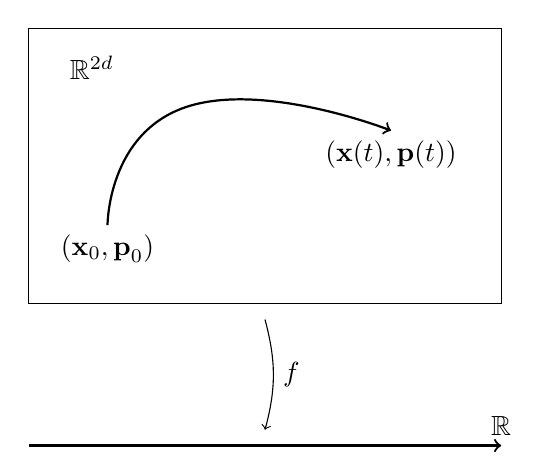
\begin{tikzpicture}
            \draw (-3,-2) rectangle (3,1.5);
            \node at (-2.2,1) {\(\RR^{2d}\)};
            \draw[->,thick] plot[smooth, tension = 1] coordinates {(-2,-1) (-1,0.5) (1.6,0.2)};
            \node at (-2,-1)[below]{\((\vb{x}_0,\vb{p}_0)\)};
            \node at (1.6,0.2)[below]{\((\vb{x}(t),\vb{p}(t))\)};
            \draw[->] (0,-2.2) to [bend left=15] node[right]{\(f\)}(0,-3.6);
            \draw[thick,->] (-3,-3.8)--(3,-3.8) node[above]{\(\RR\)};
        \end{tikzpicture}
        \caption{A particle's trajectory in phase space. Observables are represented by functions \(f:\RR^{2d}\to\RR\), evaluated along a given particle's trajectory.}
        \label{Fig:ClassicalTrajectory}
    \end{figure}

    But that is not our World. To the best of our current experimental knowledge, our world is quantum, not classical. Initially, these experiments were based on careful studies of atomic spectroscopy and blackbody radiation, but nowadays I'd prefer to say that the best evidence of quantum mechanics is simply that we use it constantly in our daily lives. Each time you listen to music on your stereo, post a photo on Instagram or make a call on your phone you're relying on technology that's only become possible due to our understanding of the quantum structure of matter. Whenever you plug something into the mains, you're using electricity that's in part generated by nuclear reactions in which quantum mechanics is essential, while much of modern medicine relies on new drugs designed with the benefit of the improved understanding of chemistry that quantum mechanics provides.

    In such a quantum world, instead of a phase space trajectory, everything we could want to know about a particle is encoded in a vector \(\psi\) in Hilbert space \(\hb\). As you met in IB Quantum Mechanics, this \textit{state vector} evolves in time according to Schr\"{o}dinger's equation. In the quantum world, observables are represented by certain operators \(\hat{O}\). The operators you saw in IB Quantum Mechanics had the same sort of form as observables in classical mechanics, such as the kinetic operator \(\hat{T}=\hat{\vb{p}}^2/2m\) or angular momentum operator \(\hat{\vb{L}}=\hat{\vb{x}}\cross\hat{\vb{p}}\). However, rather than being functions, these operators are (roughly) linear maps
    \begin{equation}
        \hat{O}:\hb\longrightarrow\hb\,.
    \end{equation}
    Again, in the first instance these operators are defined throughout \(\hb\), but if we're interested in knowing about the energy or angular momentum of our particular quantum particle, then we should find out what happens when they act on the specific \(\psi\in\hb\) that describes the state of our particle at time \(t\).

    \begin{figure}
        \centering
        \begin{tikzpicture}
            \draw (-3,-2) rectangle (3,1.5);
            \node at (-2.2,1) {\(\hb\)};
            \draw[->,thick] (-1.88,-0.96)--node[above left]{\(\hat{O}\)} (0.88,-0.04);
            \draw[fill=black] (-2,-1) circle (0.03) node[below]{\(\psi\)};
            \draw[fill=black] (1,0) circle (0.03) node[above]{\(\psi'=\hat{O}\psi\)};
        \end{tikzpicture}

        \caption{In Quantum Mechanics, complete knowledge of a particle's state is determined by a vector in Hilbert space. Observables are represented by Hermitian linear operators \(\hat{O}:\hb\to\hb\).}
    \end{figure}

    In the following chapters we'll study what Hilbert space is and what its operators do in a more general framework than you saw last year, building your insight into the mathematical structure of quantum mechanics. Much of this is just linear algebra, but the Hilbert spaces we'll care about in Quantum Mechanics are often infinite-dimensional, so we also make contact with Functional Analysis. Furthermore, although last year you `guessed' the form of quantum operators by analogy with their classical counterparts, we'll see that at a deeper level many of them can be understood to have their origins in symmetries of space and time; the operators just reflect the way these symmetry transforms act on Hilbert space, rather that on (non-relativistic) space-time. In this way, Quantum Mechanics makes contact with Representation Theory.

    So, mathematically, much of Quantum Mechanics boils down to a mix of Functional Analysis and Representation Theory. It's even true that it provides a particularly interesting example of these subjects. But this is not the reason we study it. We study Quantum Mechanics in an effort to understand and appreciate our world, not some abstract mathematical one. You're all intimately familiar with vector spaces, and you're also very good at solving Sturm--Liouville type eigenfunction/eigenvalue problems. But the real skill is in understanding how this formalism relates to the world we see around us.

    It's not obvious. Newton's laws are (at least generically) non-linear differential equations and we can't superpose solutions. General Relativity teaches us that spacetime is not flat. So it's not at all clear that our particle should in fact be described by a point in a vector space, any more than it was obvious to Aristotle that bodies actually stay in uniform motion unless acted on by a force, or clear to the Ancients that the arrival of solar eclipses, changes of the weather, or any other natural phenomenon are actually governed by calculable laws, rather than the whims of various gods. For this reason, instead of emphasizing how weird and different Quantum Mechanics is, I'd prefer to make you appreciate how it actually underpins the physics you're already familiar with. No matter how good you are at solving eigenvalue problems, if you don't see how these relate to your everyday physical intuition, knowledge you've built up since first opening your eyes and learning to crawl, then you haven't really understood the subject.

    \newpage
    \section{Hilbert Space}
    The realm of Quantum Mechanics is Hilbert space\footnote{In this course, we'll focus on Dirac's formulation of QM, which is based on Hilbert space. This is by far the most commonly used approach. However, there are some other approaches to QM (notably deformation quantization and the theory of \(C^*\)-algebra) in which Hilbert spaces do not play a prominent role. We won't discuss any of them.}, so we'll begin by exploring the properties of these. This chapter will necessarily be almost entirely mathematical; the physics comes later.

    \subsection{Definition of Hilbert Spaces}
    Hilbert space is a vector space \(\hb\) over \(\CC\) equipped with a complete inner product. Let's take a moment to understand what this means; much of it will be familiar from IB Linear Algebra or IB Methods.

    Saying that \(\hb\) is a vector space means that it is a set on which we have an operation of addition \(+:\hb\cross\hb\to\hb\), obeying
    \begin{itemize}[topsep=0pt]
        \item \textit{commutativity}. \(\psi+\phi=\phi+\psi\);
        \item \textit{associativity}. \(\psi+(\phi+\chi)=(\psi+\phi)+\chi\);
        \item \textit{identity}. \(\exists! \vb{0}\in\hb\) s.t. \(\psi+\vb{0}=\psi\)
    \end{itemize}
    for all \(\psi,\phi,\chi\in\hb\). Furthermore, we can multiply our vectors by numbers in \(\CC\) called scalars. This multiplication \(\ \cdot\ :\CC\cross\hb\to\hb\) is
    \begin{itemize}[topsep=0pt]
        \item \textit{distributive over \(\hb\)}. \(c\cdot(\psi+\phi)=c\cdot\psi+c\cdot\phi\);
        \item \textit{distributive in \(\CC\)}. \((a+b)\cdot\psi=a\cdot\psi+b\cdot\psi\)
    \end{itemize}
    for all \(a,b,c\in\CC\). In addition, \(\hb\) comes equipped with an \textit{inner product}. This is a map \((\ \ ,\ \ ):\hb\cross\hb\to\CC\) that obeys
    \begin{itemize}[topsep=0pt]
        \item \textit{conjugate symmetry}. \((\psi,\phi)=(\phi,\psi)^*\);
        \item \textit{linearity}. \((\phi,a\psi)=a(\phi,\psi)\);
        \item \textit{additivity}. \((\phi,\psi+\chi)=(\phi,\psi)+(\phi,\chi)\);
        \item \textit{positive definiteness}. \((\psi,\psi)\ge 0\), with equality iff \(\psi=\vb{0}\).
    \end{itemize}
    Note that the first two of these imply \((a\phi,\psi)=a^*(\phi,\psi)\) so that \((\ \ ,\ \ )\) is \textit{antilinear} in its first argument\footnote{In the math literature, the inner product is often taken to be linear in the first entry and antilinear in the second. We will follow the QM convention, which is opposite.}. Note also that \((\psi,\psi)=(\psi,\psi)^*\) so it is necessarily real. Whenever we have inner product, we can define the \textit{norm} of a state to be
    \begin{equation}
        \norm{\psi}=\sqrt{(\psi,\psi)}\,.
    \end{equation}
    These properties ensure that the Cauchy--Schwarz inequality
    \begin{equation}
        \abs{(\phi,\psi)}^2\le\norm{\phi}^2\norm{\psi}^2
    \end{equation}
    holds.

    As always, a set of vectors \(\{\phi_1,\phi_2,\dots,\phi_n\}\) is \textit{linearly independent} if the only solution to
    \begin{equation}
        c_1\phi_1+c_2\phi_2+\dots +c_n\phi_n=\vb{0}
    \end{equation}
    for \(c_i\in\CC\) is \(c_1=\dots=c_n=0\). The \textit{dimension} of the vector space is the largest possible number of linearly independent vectors we can find. If there is no such largest number, then we say the vector space has infinite dimension. A set of vectors \(\{\phi_1,\phi_2,\dots,\phi_n\}\) is orthonormal with respect to the inner product \((\ ,\ )\) if
    \begin{equation}
        (\phi_a,\phi_b)=\begin{cases}
        0 & \text{if }a\ne b\\
        1 & \text{if }a=b\,.
    \end{cases}
    \end{equation}
    A set \(\{\phi_1,\phi_2,\dots,\phi_n\}\) forms a \textit{basis} of an \(n\)-dimensional Hilbert space if every \(\psi\in\hb\) can be uniquely expressed as a sum
    \begin{equation}
        \psi=\sum_{i=1}^{n}c_i\phi_i\,,
    \end{equation}
    with some coefficients \(c_i\in\CC\). The basis is usually taken to be orthonormal. In this case, we can easily determine these coefficients by taking the inner product with \(\phi_i\), since
    \begin{equation}
        (\phi_i,\psi)=\left(\phi_i,\sum_{j=1}^{n}c_j\phi_j\right)=\sum_j c_j(\phi_i,\phi_j)=c_i
    \end{equation}
    by linearity and orthonormality.

    Quantum mechanics makes use of both finite and infinite dimensional Hilbert spaces, as we'll see. In the infinite dimensional case, we have to decide what we mean by an `infinite linear combination' of (e.g. basis) vectors. Not every such infinite sum makes sense, because infinite sums such as \(\sum_{i=1}^{\infty}c_i\phi_i\) might not converge. Technically, we consider the partial sums \(S_N=\sum_{i=1}^{N}c_i\phi_i\) of just the first \(N\) terms, and say that the Cauchy sequence \(\{S_1,S_2,\dots\}\) \textit{converges in the norm} if there is some vector \(\Psi\) to which it converges in the sense that
    \begin{equation}
        \lim_{N\to\infty}\norm{S_N-\Psi}=0\,.
    \end{equation}
    To say that \(\hb\) is complete (or complete in the norm) means that every Cauchy sequence \(\{S_1,S_2,\dots\}\) indeed converges in \(\hb\). This captures the heuristic idea that there are no points `missing' from \(\hb\). Importantly, it also allows us to analyse: being able to differentiate vectors in \(\hb\) requires that we can take limits, and to do this we need to know whether the limits exist.

    The interplay between the vector space structure and this requirement of completeness can be very subtle in infinite dimensions --- you'll see much more of this if you take the Part II course on Linear Analysis or (next term) Functional Analysis. In this course, we'll largely ignore such subtleties, not because they're not interesting, but because they're a distraction from all the interesting physics we need to learn.

    \subsubsection{Examples}
    Let's now look at a few examples of Hilbert spaces, pointing out where they're relevant to physics.

    The simplest case is when \(\hb\) is finite dimensional. In this case, as a vector space we have \(\hb\cong\CC^n\) for some \(n\). You might think we still have lots of choice in picking an inner product, but it turns out that finite dimensional Hilbert space is always isomorphic to one with inner product
    \begin{equation}
        (\vb{v},\vb{u})=\sum_{i=1}^{n}v_i^*u_i
    \end{equation}
    and corresponding norm
    \begin{equation}
        \norm{u}=\sqrt{\sum_{i=1}^{n}\abs{u_i}^2}\,.
    \end{equation}
    Here \(\{u_i\}\) are just complex numbers --- the components of the vector \(\vb{u}\) in the canonical basis.

    In physics, finite dimensional Hilbert spaces often arise as idealizations or ``toy models''. We may wish to illustrate some quantum phenomenon by first considering an especially simple case that has only finitely many (perhaps just two) different things it can do. Alternatively, we may be concerned with just a finite dimensional subspace of a larger physical system. For example, we may be interested in states at a particular energy level of a degenerate Hamiltonian, which can easily be finite dimensional. Also, we'll see later that the angular behavior of systems with a fixed (and finite) total angular momentum is also captured by a finite dimensional Hilbert space.

    A simple infinite dimensional generalisation of this is the space of infinite sequences of complex number \(\vb{u}=(u_1,u_2,\dots)\) such that
    \begin{equation}
        \sum_{i=1}^{\infty}\abs{u_i}^2<\infty\,.
    \end{equation}
    This space is known as \(\ell^2\) and, heuristically, you can think of it as ``\(\CC^n\) with \(n=\infty\)''. The inner product between two such sequences \(\vb{u}\) and \(\vb{v}\) is defined as
    \begin{equation}
        (\vb{v},\vb{u})=\sum_{i=1}^{\infty}v_i^* u_i
    \end{equation}
    as an obvious generalisation of the finite dimensional case. The Cauchy--Schwarz inequality gives \(\abs{(\vb{v},\vb{u})}\le\norm{\vb{v}}\norm{\vb{u}}<\infty\), so this inner product converges provided the norms do. Again, the notion of completeness of \(\ell^2\) with respect to this norm enables us to meaningfully take limits and, ultimately, differentiate vectors \(\vb{u}\in \ell^2\).

    In physics, \(\ell^2\) arises in many places. For example, the space of energy eigenstates in an infinite square well, or in the harmonic oscillator potential, may be thought of \(\ell^2\). Similarly, the space of \textit{bound states} (\(E<0\)) of the hydrogen atom is \(\ell^2\), though the scattering states (\(E\ge 0\)) are not.

    We'll often also meet infinite dimensional vector spaces that are spaces of functions, such as the wavefunctions you dealt with throughout IB Quantum Mechanics. Given two functions \(\psi,\phi:\RR\to\CC\), we can define linear combinations \(a\psi+b\phi\) for any \(a,b\in\CC\) in the obvious way
    \begin{equation}
        (a\psi+b\phi)(x)=a\psi(x)+b\phi(x)\,,
    \end{equation}
    where the multiplication and addition on the right-hand side are just those in \(\CC\), so spaces of functions are naturally infinite dimensional vector spaces (as you saw in IB Methods). To turn this space of functions into a Hilbert space, we first give it the norm
    \begin{equation}\label{function_L2_norm}
        \norm{\psi}=\sqrt{\int_\RR\dd{x}\abs{\psi(x)}^2}
    \end{equation}
    and require that \(\norm{\psi}<\infty\), i.e. the integral converges. In physics, functions for which \(\norm{\psi}<\infty\) holds are called \textit{normalisable}. Note that just asking (\ref{function_L2_norm}) to converge is not a very strong restriction, and so our normed function space contains a very wide class of functions, including all piecewise continuous functions that decay sufficiently rapidly as \(\abs{x}\to\infty\), and even some functions that are singular for some discrete values of \(x\), provided these singularities are not strong enough to cause the integral to diverge\footnote{The requirement that the space be complete in the norm (\ref{function_L2_norm}) is rather subtle. If \(\norm{\psi-\phi}=0\), then we must identify \(\psi\) and \(\phi\) as the same object in our space. This does not necessarily mean that they're identical as functions, because e.g. they could take different at some discrete points \(x_i\subset \RR\), as the non-zero value of \(\psi-\phi\) at these discrete points would not contribute to the norm (\ref{function_L2_norm}). In particular, any function that is non-zero only at a set of points that has a \textit{Lebesgue measure} zero should be identified with the zero function. The resulting space is known as \(L^2(\RR,\d{x})\) or sometimes just \(L^2\) for short. (The \(L\) stands for Lebesgue, and is an example of a more general type of normed function space.) \(L^2(\RR,\d{x})\) consists of equivalence classes of Cauchy sequences of functions that are convergent in the norm. In this course we'll mostly gloss over such technicalities, and they're certainly non-examinable. For a deeper discussion of Hilbert space, see the Part II Linear Analysis and Functional Analysis courses.}.

    Finally, we take the inner product between two functions \(\psi\) and \(\phi\) whose norms are finite to be
    \begin{equation}
        (\phi,\psi)=\int_\RR\dd{x}\phi(x)^*\psi(x)\,,
    \end{equation}
    and again this converges by Cauchy--Schwarz. In physics, we often call \(\psi(x)\) the \textit{wavefunction} of the particle, and sometimes call \((\phi,\psi)\) the \textit{overlap integral} between two wavefunctions.
    \subsubsection{Dual Spaces}
    As with any vector space, the \textit{dual} \(\hb^*\) of a Hilbert space \(\hb\) is the space of linear maps \(\hb\to\CC\). That is, an element \(\varphi\in\hb^*\) defines a map \(\varphi:\psi\mapsto\varphi(\psi)\) for every \(\psi\in\hb\), such that
    \begin{equation}
        \varphi:a\psi_1+b\psi_2\longmapsto a\varphi(\psi_1)+b\varphi(\psi_2)
    \end{equation}
    for all \(\psi_1,\psi_2\in\hb\) and \(a,b\in\CC\).

    One way to construct such a map is to use the inner product. Given some state \(\phi\in\hb\), we can define an element \((\phi,\ \ )\in\hb^*\) which acts on \(\psi\in\hb\) by
    \begin{equation}
        (\phi,\ \ ):\psi\longmapsto(\phi,\psi)\,,
    \end{equation}
    i.e. we take the inner product of \(\psi\in\hb\) with our chosen element \(\phi\). The linearity properties of the inner product transfer to ensure that \((\phi,\ \ )\) is indeed a linear map --- note that since the inner product is antilinear in its first entry, it's important that our chosen element \(\phi\) to sit in this first entry. In IB Linear Algebra you proved that, in finite dimensions, every element of \(\hb\) arises this way. That is, any linear map \(\varphi:\hb\to\CC\) can be written as \((\phi,\ \ )\) for some \(\phi\in\hb\). This means in particular that the inner product \((\ ,\ )\) provides a vector space isomorphism
    \begin{align}
        \hb&\cong\hb^*\,, \notag\\
        \phi&\leftrightarrow (\phi,\ \ )=\phi^\dagger\,.
    \end{align}
    The notation \(^\dagger\) is known as the \textit{Hermitian conjugate} that transform a vector \(\phi\in\hb\) into its dual \(\phi^\dagger\in\hb\). Comfortingly, the same result also holds in infinite dimensions\footnote{We should really be more careful here, though we won't be concerned with the following subtleties in this course. In infinite dimensions we distinguish the \textit{algebraic dual space} --- the space of all linear functionals \(\varphi:H\to\CC\) from the \textit{continuous dual}, where the number \(\varphi(\psi)\) is required to vary continuously as \(\psi\) varies in \(\hb\). The Riesz Representation Theorem applies to the continuous dual. For example, the algebraic dual also contains distributions such as the Dirac delta, \(\delta\), acting as \(\delta:\psi\mapsto\psi(\vb{0})\)``\(=\int_\RR\dd{x}\delta(x)\psi(x)\)'', with \(\psi\in L^2(\RR,\d{x})\). Certainly \(\delta(x)\) is not itself square-integrable, so is not in the Hilbert space. However, since \(L^2(\RR,\dd{x})\) contains discontinuous functions, \(\delta[\psi]\) does not have to vary smoothly with \(\psi\). Functional analysis is almost always interested in the continuous dual, and thus this is often called just the \textit{dual space}.}, but it's non-trivial to prove and is known as the \textit{Riesz Representation Theorem}. The isomorphism \(\hb^*\cong\hb\) is what is special about Hilbert spaces among various other infinite dimensional vector spaces, and makes them especially easy to handle.
    \subsubsection{Dirac Notation and Continuum States}
    From now on, in this course we'll use a notation for Hilbert spaces that was introduced by Dirac and is standard throughout the theoretical physics literature. Dirac denotes an element of \(\hb\) as \(\ket{\psi}\), where the symbol ``\(\ket{\ \ }\)'' is known as a \textit{ket}. An element of the dual space is written \(\bra{\phi}\) and the symbol ``\(\bra{\ \ }\)'' is called a \textit{bra}. The relation between the ket \(\ket{\phi}\in\hb\) and the bra \(\bra{\phi}\in\hb^*\) is what we would previously have written as \(\phi\) versus \((\phi,\ )\). We can again use Hermitian conjugate to transform a ket into a bra: \(\ket{\phi}^\dagger\equiv\bra{\phi}\), or vice versa, \(\bra{\phi}^\dagger\equiv\ket{\phi}\). The inner product between two states \(\ket{\psi},\ket{\phi}\in\hb\) is then written \(\braket{\phi}{\psi}\) forming a \textit{bra-ket} or bracket. Note that everything above implicitly uses the isomorphism \(\hb^*\cong\hb\) provided by the inner product, building it into the notation. Recall also that in all physics courses, \(\braket{\phi}{\psi}\) is antilinear in \(\bra{\phi}\).

    Given an orthonormal basis \(\{\ket{e_i}\}\) of \(\hb\), at least in the cases \(\hb\cong\CC^n\) or \(\hb\cong \ell^2\), in Dirac notation we can expand a general ket \(\ket{\psi}\in\hb\) as
    \begin{equation}\label{orthonormal_basis_expansion}
        \ket{\psi}=\sum_i \psi_i\ket{e_i}
    \end{equation}
    in terms of this basis. Then the inner product of \(\chi,\psi\in\hb\) can be expanded as
    \begin{equation}
        \braket{\chi}{\psi}=\sum_{i,j}\chi_j^*\psi_i\braket{e_j}{e_i}=\sum_i \chi_i^*\psi_i
    \end{equation}
    as usual.

    It's very useful to be able to extend this idea also to function spaces. In this case, we introduce a \textit{continuum basis} with elements \(\ket{a}\) labelled by a continuous variable \(a\), normalised so that
    \begin{equation}\label{continuum_basis_normalisation}
        \braket{a'}{a}=\delta(a'-a)
    \end{equation}
    using the Dirac \(\delta\)-function. To expand a \(\ket{\psi}\) in a continuum basis, we need to replace the summation in (\ref{orthonormal_basis_expansion}) and write
    \begin{equation}
        \ket{\psi}=\int\dd{a}\psi(a)\ket{a}\,,
    \end{equation}
    where \(\psi(a)\) is the component of \(\ket{a}\). The point of the normalisation (\ref{continuum_basis_normalisation}) is that
    \begin{equation}
        \braket{\chi}{\psi}=\int\dd{b}\int\dd{a}\chi(b)^*\psi(a)\braket{b}{a}=\int\dd{b}\int\dd{a}\chi(b)^*\psi(a)\delta(b-a)=\int\dd{a}\chi(a)^*\psi(a)\,,
    \end{equation}
    which is just the inner product (and also norm) we defined for \(L^2(\RR,\d{a})\) before. Indeed, a key example of a continuum basis is the \textit{position basis} \(\{\ket{x}\}\), where \(x\in\RR\). Expanding a general state \(\ket{\psi}\) as an integral gives
    \begin{equation}
        \ket{\psi}=\int_\RR\dd{x'}\psi(x')\ket{x'}\,.
    \end{equation}
    We see that the complex coefficients are
    \begin{equation}
        \braket{x}{\psi}=\int_\RR\dd{x'}\psi(x')\braket{x}{x'}=\psi(x)\,.
    \end{equation}
    In other words, the position space wavefunctions we're familiar with are nothing but the coefficients of a state \(\ket{\psi}\in\hb\) in a particular position continuum basis.

    As always, we could equally choose to expand this same vector in different bases. For example, our state \(\ket{\psi}=\int_\RR\dd{x}\psi(x)\ket{x}\) from above can equally be expanded in the momentum basis as \(\ket{\psi}=\int_{\tilde{\RR}} \dd{p}\tilde{\psi}(p)\ket{p}\), where the new coefficients \(\tilde{\psi}(p)=\braket{p}{\psi}\) are the \textit{momentum space wavefunction}. Later, we'll show that \(\braket{x}{p}=\ee^{\ii xp/\hbar}/\sqrt{2\pi\hbar}\), so these two sets of coefficients are related by
    \begin{align}\label{xp_coefficient_relation}
        \braket{x}{\psi}&=\int_{\tilde{\RR}}\dd{p}\tilde{\psi}(p)\braket{x}{p}=\frac{1}{\sqrt{2\pi\hbar}}\int_{\tilde{\RR}}\dd{p}\ee^{\ii xp/\hbar}\tilde{\psi}(p)\,,\\
        \braket{p}{\psi}&=\int_{\RR}\dd{x}\psi(x)\braket{p}{x}=\frac{1}{\sqrt{2\pi\hbar}}\int_{\RR}\dd{x}\ee^{-\ii xp/\hbar}\psi(x)\,.\label{px_coefficient_relation}
    \end{align}
    \Cref{xp_coefficient_relation,px_coefficient_relation} are just the statements that the position and momentum space wavefunctions are each other's Fourier transforms, again familiar from IB Quantum Mechanics.

    The real point I wish to make is that the fundamental object is the abstract vector \(\ket{\psi}\in\hb\). All the physical information about a quantum system is encoded in its state vector \(\ket{\psi}\); the wavefunctions \(\psi(x)\) or \(\tilde{\psi}(p)\) are merely the expansion coefficients in some basis. Like any other choice of basis, this expansion may be useful for some purposes and unhelpful for others.

    Finally, a technical point. Although using continuum bases such as \(\{\ket{x}\}\) and \(\{\ket{p}\}\) is convenient, because it emphasizes the similarities between the finite and infinite-dimensional cases, it blurs the analysis. In particular, if \(\braket{x'}{x}=\delta(x'-x)\) then the norm
    \begin{equation}
        \norm{\ket{x}}^2=\delta(x-x)=\delta(0)\,.
    \end{equation}
    So whatever these objects \(\ket{x}\) are, they certainly do not lie in our Hilbert space. It is possible to make good mathematical sense of these by appropriately enlarging our spaces to include spaces of distributions, but for the most part (and certainly in this course) physicists are content to say that continuum states such as \(\ket{x}\) are allowable as basis elements, but call them non-normalizable states: actual physical particles are never represented by a non-normalizable state.

    \subsection{Operators}
    A \textit{linear operator} \(A\) is a map \(A:\hb\to\hb\) that is compatible with the vector space structure in the sense that
    \begin{equation}
        A(c_1\ket{\psi_1}+c_2\ket{\psi_2})=c_1A\ket{\psi_1}+c_2A\ket{\psi_2}
    \end{equation}
    in Dirac notation\footnote{Here we are being a little sloppy again. In the infinite dimensional case, it often happens that operators are not defined on the whole of \(\hb\), but just on some domain \(\Dom A\subseteq\hb\) which depends on the operator itself. For example, the momentum operator \(P\) acts on position space wavefunctions \(\psi(x)\in L^2(\RR,\dd{x})\) by \(-\ii\hbar\partial/\partial x\). If \(\psi(x)\) is discontinuous, then it could be that \(\int\dd{x}\abs{\psi'}^2\) diverges even though \(\int\dd{x}\abs{\psi}^2\) itself is finite. Understanding the correct domain of various operators is an important part of functional analysis. We'll largely ignore such subtleties in this course.}. All the operators we meet in Quantum Mechanics will be linear, so henceforth we'll just call them ``operators''. Operators form an algebra: given two such linear operators \(A\), \(B\), we define their sum \(\alpha A+\beta B\) as
    \begin{equation}
        (\alpha A+\beta B):\ket{\psi}\mapsto \alpha A\ket{\psi}+\beta B\ket{\psi}
    \end{equation}
    for all \(\alpha,\beta\in\CC\) and all \(\ket{\psi}\in\hb\), and take their product \(AB\) to be the composition
    \begin{equation}
        AB:\ket{\psi}\mapsto A\circ B\ket{\psi}\equiv A(B\ket{\psi})
    \end{equation}
    for \(\ket{\psi}\in\hb\). One can check that both the sum and product of two linear operators is
    again a linear operator\footnote{A linear operator is \textit{bounded} if, for all \(\ket{\psi}\in\hb\),
    \begin{equation}
        \norm{A\ket{\psi}}\le M\norm{\ket{\psi}}
    \end{equation}
    for some \(M>0\). The space of such bounded linear operators on \(\hb\) is denoted as \(B(\hb)\). Bounded linear operators thus map normalisable states to normalisable states, and so act on the whole Hilbert space \(\hb\). This usually makes them the nicest ones to deal with. One of the reasons we'll be largely ignoring the analysis aspects of Hilbert space in this course is that the operators we commonly deal with in quantum mechanics, such as the position and momentum operators X and P, are unbounded. (For example, even when its wavefunction is correctly normalised, a particle can be located at arbitrarily large \(\vb{x}\in\RR^3\), or have arbitrarily large momentum.) It's of course possible to handle such unbounded operators rigorously, but doing so involves an extra layer of technicality that would take us too far afield here. For further discussion, see that Part II course on Analysis of Functions.}.

    The operator algebra is associative, so \(A(BC)=(AB)C\), but not commutative and in general \(AB\ne BA\) so the order in which the operators act is important. The difference between these two actions is known as the \textit{commutator}
    \begin{equation}
        [A,B]=AB-BA\,.
    \end{equation}
    The commutator obeys the following properties:
    \begin{itemize}[topsep=0pt]
        \item \textit{anti-symmetry}. \([A,B]=-[B,A]\);
        \item \textit{linearity}. \([\alpha_1A_1+\alpha_2A_2,B]=\alpha_1[A_1,B]+\alpha_2[A_2,B]\ \forall\alpha_1,\alpha_2\in\CC\);
        \item \textit{Leibniz identity}. \([A,BC]=[A,B]C+B[A,C]\);
        \item \textit{Jacobi identity}. \([A,[B,C]]+[B,[C,A]]+[C,[A,B]]=0\).
    \end{itemize}
    These are easy to verify from the definitions. Commutators of operators arise frequently in quantum mechanics.

    A state \(\ket{\psi}\in\hb\) is said to be an \textit{eigenstate} of an operator \(A\) if
    \begin{equation}
        A\ket{\psi}=\lambda\ket{\psi}\,,
    \end{equation}
    where the number \(\lambda\in\CC\) is known as its \textit{eigenvalue}. Thus, if \(\ket{\psi}\) is an eigenstate of \(A\), acting on \(\ket{\psi}\) with \(A\) returns exactly the same vector, except that it is rescaled by a number that may depend both on the state and the particular operator. The set of all eigenvalues of an operator \(A\) is sometimes called the \textit{spectrum} of \(A\), while the number of linearly independent eigenstates having the same eigenvalue is called the degeneracy of this eigenvalue.

    One place where Dirac notation is particularly convenient is that it allows us to label states by their eigenvalues. We let \(\ket{q}\) denote an eigenstate of some operator \(Q\) with eigenvalue \(q\), so that \(Q\ket{q}=q\ket{q}\). For example, a state that is an eigenstate of the position operator \(\vb{X}\) with position \(\vb{x}\in\RR^3\) (representing a particle that is definitely located at \(\vb{x}\)) is written \(\ket{\vb{x}}\), while the state \(\ket{\vb{p}}\) is an eigenstate of the momentum operator \(\vb{P}\) with eigenvalue \(\vb{p}\). There's a potential confusion here: \(\ket{\vb{x}}\) does not refer to the function \(\vb{x}\), but rather a state in \(\hb\) whose only support is at \(\vb{x}\). We saw above that the wavefunction corresponding to \(\ket{\vb{x}}\) was really a \(\delta\) function.

    In this course, I'll mostly use the convention that operators are written using capital letters, with their eigenvalues being labelled by the same letter in lowercase. However, I won't stick to this religiously; a notable and deeply ingrained exception is to use \(E\) for the eigenvalues of the Hamiltonian operator \(H\).

    The extra structure of the inner product on \(\hb\) allows us to also define the \textit{Hermitian conjugate} or \textit{adjoint} \(A^\dagger\) of an operator \(A\) by
    \begin{equation}
        \bra{\phi}A^\dagger=\left(A\ket{\phi}\right)^\dagger\,,
    \end{equation}
    or, equivalently,
    \begin{equation}
        \mel{\phi}{A^\dagger}{\psi}=\left(A\ket{\phi}\right)^\dagger\ket{\psi}=\mel{\psi}{A}{\phi}^*
    \end{equation}
    for all \(\ket{\phi},\ket{\psi}\in\hb\). One can easily check that\footnote{At least for the finite dimensional case. We'll assume without being careful that it holds in the infinite dimensional case too.}
    \begin{equation}
        (A+B)^\dagger=A^\dagger+B^\dagger\,,\;(AB)^\dagger=(BA)^\dagger\,,\;(\alpha A)^\dagger=\alpha^*A^\dagger\text{ and }(A^\dagger)^\dagger=A\,,
    \end{equation}
    from which it follows that \([A,B]^\dagger=[B^\dagger,A^\dagger]\). Note also that the adjoint of the eigenvalue equation \(A\ket{a}=a\ket{a}\) is
    \begin{equation}
        \bra{a}A^\dagger=\bra{a}a^*\,,
    \end{equation}
    where \(A^\dagger\) is taken to act to the left on the dual vector \(\bra{a}\).

    An operator \(Q\) is called \textit{Hermitian}\footnote{The terminology \textit{Hermitian} is used in the physics literature, coming from the fact that if \(\hb\) is finite dimensional, we can represent linear operators obeying \(Q^\dagger=Q\) by Hermitian matrices. In functional analysis, we'd have to be a little more careful about exactly which states we allow our operator to act on. For example, differentiating a non-smooth but square-integrable function will typically sharpen its singularities and may render it non-normalisable. Thus the momentum operator \(-\ii\hbar\mathrm{d}/\mathrm{d}x\) may take a state in \(\hb\cong L^2(\RR,\d{x})\) out of \(L^2(\RR,\d{x})\), and to keep analytic control we should first limit the states on which we allow the momentum operator to act. Being more careful, we'd say that operators obeying \(\bra{\psi}Q\ket{\phi}=\bra{\phi}Q\ket{\psi}^*\) for all \(\ket{\phi},\ket{\psi}\in\Dom Q\subseteq\Dom Q^\dagger\subseteq\hb\) and \(\Dom Q\) dense in \(\hb\) are \textit{symmetric}, while symmetric operators for which \(\Dom Q=\Dom Q^\dagger\) are called \textit{self-adjoint}. The distinction between operators that are self-adjoint and those that are merely symmetric is a little technical, but has important consequences for their spectrum and the existence of eigenstates. See e.g. \textcolor{blue}{\href{https://en.wikipedia.org/wiki/Self-adjoint_operator}{this Wikipedia page}} for a basic discussion with examples. We'll largely ignore such subtleties in our course.} if \(Q^\dagger=Q\), so that \(\mel{\phi}{Q}{\psi}=\mel{\psi}{Q}{\phi}^*\) for all \(\ket{\phi},\ket{\psi}\in\hb\). Hermitian operators are very special and have a number of important properties. Firstly, suppose \(\ket{q}\) is an eigenstate of a Hermitian operator \(Q\) with eigenvalue \(q\), then
    \begin{equation}
        q\braket{q}{q}=\mel{q}{Q}{q}=\bra{q}Q\ket{q}^*=q^*\braket{q}{q}\,,
    \end{equation}
    so \(q=q^*\). Hence, the eigenvalues of a Hermitian operator are real. Second, suppose \(\ket{q_1}\) and \(\ket{q_2}\) are both eigenstates of \(Q\) with distinct eigenvalues \(q_1\) and \(q_2\). Then
    \begin{equation}
        (q_1-q_2)\braket{q_1}{q_2}=\bra{q_1}Q^\dagger\ket{q_2}-\bra{q_1}Q\ket{q_2}=0\,,
    \end{equation}
    where the first equality uses the fact that \(q_1\) is real and the second uses the fact that \(Q\) is Hermitian. Since \(q_1\ne q_2\) by assumption, we must have \(\braket{q_1}{q_2}=0\), so the eigenstates of Hermitian operators with distinct eigenvalues are orthogonal, and after rescaling, we can choose them to be orthonormal.

    In the finite dimensional case, you proved in IB Linear Algebra that the set of eigenvectors of a given Hermitian operator form a basis of \(\hb\); that is, they form a complete, orthonormal set. This property allows us to express Hermitian operators in a form that is often useful. If \(\{\ket{n}\}\) is an orthonormal basis of eigenstates of a Hermitian operator \(Q\), with eigenvalues \(\{\lambda_n\}\), then we can write
    \begin{equation}
        Q=\sum_n\lambda_n\ket{n}\bra{n}\,,
    \end{equation}
    where we think of this as acting on \(\ket{\psi}\in\hb\) by
    \begin{equation}
        Q\ket{\psi}=\sum_n \lambda_n \ket{n}\braket{n}{\psi}\,.
    \end{equation}
    Note that indeed \(Q\ket{n}\in\hb\), since the \(\braket{n}{\psi}\) are just numbers in \(\CC\), whereas each term in the sum also involves \(\ket{n}\in\hb\). In particular, expressing \(\ket{\psi}\) in this basis as \(\ket{\psi}=\sum_m c_m\ket{m}\) gives
    \begin{equation}
        Q\ket{\psi}=\sum_{n,m}\lambda_n c_m\ket{n}\braket{n}{m}=\sum_n \lambda_n c_n\ket{n}\,.
    \end{equation}

    One reason this representation of \(Q\) is useful is that it allows us to define functions of operations. We set
    \begin{equation}\label{function_of_operator}
        f(Q)=\sum_n f(\lambda_n)\ket{n}\bra{n}\,,
    \end{equation}
    provided \(f(\lambda_n)\) is defined for all eigenvalues \(\lambda_n\) of the original operator. For example, the inverse of an operator \(Q\) is the operator
    \begin{equation}
        Q^{-1}=\sum_n \frac{1}{\lambda_n}\ket{n}\bra{n}
    \end{equation}
    provided \(\lambda_n\ne 0\) for all \(n\), while
    \begin{equation}
        \ln Q=\sum_n\ln(\lambda_n)\ket{n}\bra{n}
    \end{equation}
    when the eigenvalues of \(Q\) are all positive.

    A particularly important example of this is that we can represent the identity operator \(\Id\) on \(\hb\) as
    \begin{equation}
        \Id=\sum_n\ket{n}\bra{n}\text{ or }\Id=\int\dd{q}\ket{q}\bra{q}\,,
    \end{equation}
    where \(\{\ket{n}\}\) or \(\{\ket{q}\}\) are any bases of \(\hb\) respectively for discrete or continuous labels. This is often convenient for moving between different bases. For example, if \(\{\ket{p}\}\) denotes a complete set of eigenstates of the momentum operator \(P\), with \(P\ket{p}=p\ket{p}\), then to represent this operator acting on a state \(\ket{\psi}\) in the position basis we write
    \begin{align}
        \mel{x}{P}{\psi}&=\int\dd{p}\mel{x}{P}{p}\braket{p}{\psi}=\int\dd{p}\braket{x}{p}p\tilde{\psi}(p) \notag \\
        &=\frac{1}{\sqrt{2\pi\hbar}}\int\dd{p}\ee^{\ii xp/\hbar}p\tilde{\psi}(p)=-\ii\hbar\pdv{}{x}\left[\frac{1}{\sqrt{2\pi\hbar}}\int\dd{p}\ee^{\ii xp/\hbar}\tilde{\psi}(p)\right]\,.
    \end{align}
    In the first equality here we've squeezed the identity operator \(\Id=\int\dd{p}\ket{p}\bra{p}\) in between the momentum operator \(P\) and the general state \(\ket{\psi}\), then used the fact that \(\ket{p}\) is an eigenstate of \(P\), and finally used our previous expression for \(\braket{x}{p}\) and standard properties of Fourier transforms. We recognise the integral in the final expression as the position space wavefunction of \(\ket{\psi}\), so altogether we have
    \begin{equation}
        \mel{x}{P}{\psi}=-\ii\hbar\pdv{}{x}\braket{x}{\psi}\,,
    \end{equation}
    or \(\hat{P}\psi(x)=-\ii\hbar\partial\psi/\partial x\) in IB notation. This and similar manipulations will be used repeatedly throughout the course, so it's important to make sure you're comfortable with them.

    If \(\hb\) is finite dimensional, we can represent any linear operator on \(\hb\) by a matrix. We pick an orthonormal basis \({\ket{n}}\) and define
    \begin{equation}
        A_{nm}=\mel{n}{A}{m}
    \end{equation}
    as usual. In particular, inserting the identity operator in the form \(\Id=\sum_n\ket{n}\bra{n}\) shows that the matrix elements of the product operator \(AB\) as
    \begin{align}
        (AB)_{km}&=\mel{k}{AB}{m}=\mel{k}{A\left(\sum_n\ket{n}\bra{n}\right)B}{m} \notag\\
        &=\sum_n\mel{k}{A}{n}\mel{n}{B}{m}=\sum_n A_{kn}B_{nm}\,,
    \end{align}
    which just corresponds to usual matrix multiplication. Hermitian operators are represented by Hermitian matrices, i.e. ones whose elements obey \((\mathsf{A}^\dagger)_{mn}\coloneqq A_{nm}^*=A_{mn}\), hence the name.
    \subsection{Composite Systems}\label{Chap:Composite_Systems}
    We often have to deal with systems with more than a single degree of freedom. This could be just a single particle moving in three dimensions rather than one, or a composite system such as a hydrogen atom consisting of both an electron and a proton, or a diamond which consists of a very large number of carbon atoms. In the case of a macroscopic object, our system could be made up of a huge number of constituent parts, each able to behave differently, at least in principle.

    It should be intuitively clear that the more complicated our system is, meaning the more independent degrees of freedom it possesses, the larger a Hilbert space we'll need if we wish to encode all its possible states. We'll now understand how quantum mechanics handles systems with more than one degree of freedom by taking the tensor product of the Hilbert spaces of its constituent parts.

    \subsubsection{Tensor Product of Hilbert Spaces}
    Hilbert spaces are vector spaces over \(\CC\), so we can try to define their tensor product in the same way as we would for any pair of vector spaces. Recall from IB Linear Algebra that if \(\hb_1\) and \(\hb_2\) are two finite Hilbert spaces, with \(\{\ket{e_a}\}_{a=1}^{m}\) a basis of \(\hb_1\) and \(\{\ket{f_\alpha}\}_{\alpha=1}^{n}\) a basis of \(\hb_2\), then the \textit{tensor product space} \(\hb_1\otimes\hb_2\) is again a vector space over \(\CC\) spanned by all pairs of elements \(\ket{e_a}\otimes\ket{f_\alpha}\) chosen from the two bases\footnote{If you're a purist (and the PQM Tripos examiners are not), then there's something slightly unsatisfactory about this definition of the tensor product vector space, which is that it apparently depends on a choice of basis on both \(\hb_1\) and \(\hb_2\). We can do better, just using the abstract vector space structure, as follows. For any pair of vector spaces \(V\) and \(W\), we first define the \textit{free vector space} \(F(V\times W)\) to be the set of all possible pairs of elements chosen from \(V\) and \(W\). This is a vector space with the sum of a pair \((v,w)\) and a pair \((v',w')\) denoted simply by \((v,w)+(v',w')\) (Do not confuse the pair \((v,w)\in F(V\cross W)\) with an inner product! Here \(v\) and \(w\) live in different spaces.) By itself, \(F(V\cross W)\) does not care that \(V\) and \(W\) are already vector spaces. For example, if \({e_i}\) is a basis for \(V\) and \(v=c_1e_1+c_2e_2\) for some coefficients \(c_1,c_2\), the elements \((v,w)\) and \(c_1(e_1,w)+c_2(e_2,w)\) are nonetheless distinct in \(F(V\cross W)\). We'd like to teach the free vector space about the structure inherited from \(V\) and \(W\) individually. We thus define the tensor product \(V\otimes W\) to be the \textit{quotient} \(F(V\cross W)/\sim\) under the equivalence relations
    \begin{equation}
        (v,w)+(v',w)\sim(v+v',w)\,,\; (v,w)+(v,w')\sim(v,w+w')\text{ and } c(v,w)\sim(cv,w)\sim(v,cw)
    \end{equation}
    for all \(v\in V\), \(w\in W\) and \(c\in\CC\). We denote the equivalence class of the pair \((v,w)\) by \(v\otimes w\).}. It follows that
    \begin{equation}
        \dim(\hb_1\otimes\hb_2)=\dim(\hb_1)\dim(\hb_2)
    \end{equation}
    provided these are finite. This should be familiar from IB Linear Algebra.

    It's important to stress that, as with any vector space, a general element of \(\hb_1\otimes\hb_2\) is a linear combination of its basis elements \(\ket{e_a}\otimes\ket{f_\alpha}\). In particular, although general elements of \(\hb_1\) and \(\hb_2\) can be written
    \begin{equation}
        \ket{\psi_1}=\sum_{a=1}^{m}c_a\ket{e_a}\quad\text{and}\quad\ket{\psi_2}=\sum_{\alpha=1}^{n}d_\alpha\ket{f_\alpha}\,,
    \end{equation}
    it is not true that a general element of \(\hb_1\otimes\hb_2\) necessarily takes the form
    \begin{equation}
        \ket{\psi_1}\otimes\ket{\psi_2}=\sum_{a,\alpha}c_ad_\alpha\ket{e_a}\otimes\ket{f_\alpha}\,.
    \end{equation}
    Rather, a general element of \(\hb_1\otimes\hb_2\) is written as
    \begin{equation}\label{entangled_element_form}
        \ket{\Psi}=\sum_{a,\alpha}r_{a,\alpha}\ket{e_a}\otimes\ket{f_\alpha}\,.
    \end{equation}
    In particular, elements of the form \(\ket{\psi_1}\otimes\ket{\psi_2}\in\hb_1\otimes\hb_2\) are only specified by \(\dim\hb_1+\dim\hb_2\) coefficients, vastly fewer than is required to specify a generic element. Elements of the form \(\ket{\psi}\otimes\ket{\phi}\) are sometimes called simple, while in physics generic elements of the form (\ref{entangled_element_form}) are said to be entangled. In \cref{Chap:Interpreting_QM} we'll explore some of the vast resources this entanglement opens up to quantum mechanics; you'll see much more of it next term if you take the course on Quantum Information and Computation.

    In order to make \(\hb_1\otimes\hb_2\) a Hilbert space, rather than just a vector space, we must give it an inner product. We do this in the obvious way. Let \(\braket{\ \ }{\ \ }_1\) and \(\braket{\ \ }{\ \ }_2\) denote inner products on \(\hb_1\) and \(\hb_2\). We first define the inner product between each pair of basis elements of \(\hb_1\otimes\hb_2\) by
    \begin{equation}
        (\bra{e_a}\otimes\bra{f_\alpha})(\ket{e_b}\otimes\ket{f_\beta})=\braket{e_a}{e_b}_1\braket{f_\alpha}{f_\beta}_2\,,
    \end{equation}
    and then extend it to arbitrary states \(\ket{\Psi}\) by linearity. Note in particular that if \(\{\ket{e_a}\}\) and \(\{f_\alpha\}\) are orthonormal bases of their respective Hilbert spaces, then \(\{\ket{e_a}\otimes\ket{f_\alpha}\}\) will be an orthonormal basis of \(\hb_1\otimes\hb_2\).

    The most common occurrence of this is simply a single particle moving in more than one dimension. For example, suppose a quantum particle moves in \(\RR^2\), described by Cartesian coordinates \((x,y)\). If \(\{\ket{x}\}_{x\in\RR}\) is a complete set of position eigenstates for the \(x\)-direction, and \(\{\ket{y}\}_{y\in\RR}\) is likewise a complete set for the \(y\)-direction, then the state of the particle can be expanded as
    \begin{equation}
        \ket{\psi}=\int_{\RR\times\RR}\dd{x}\dd{y}\psi(x,y)\ket{x}\otimes\ket{y}\,,
    \end{equation}
    where \(\{\ket{x}\otimes\ket{y}\}_{x,y\in\RR}\) form a continuum basis of the tensor product space. Note that in general, our wavefunction is not a simple product \(\psi(x,y)\ne\psi_1(x)\psi_2(y)\) of wavefunctions in the two directions separately, though it may be possible to write it as the sum of such products, as you met repeatedly when studying the separation of variables in IB Methods. In this continuum case, the inner product between any two states is
    \begin{align}
        \braket{\chi}{\psi}&=\int_{\RR^2\times\RR^2}\dd{x'}\dd{y'}\dd{x}\dd{y}\chi(x',y')^*\psi(x,y)\braket{x'}{x}\braket{y'}{y}\notag\\
        &=\int_{\RR^2\times\RR^2}\dd{x'}\dd{y'}\dd{x}\dd{y}\chi(x',y')^*\psi(x,y)\delta(x-x')\delta(y-y')\notag\\
        &=\int_{\RR^2}\dd{x}\dd{y}\chi(x,y)^*\psi(x,y)\,.
    \end{align}
    This is exactly the structure of \(L^2(\RR^2,\d[2]{\vb{x}})\), and we identify\footnote{There is actually one more step in the infinite dimensional case: we must take the \textit{completion} of \(L^2(\RR,\d{x})\otimes L^2(\RR,\d{y})\) in the norm associated to this inner product. There is no problem if our general state \(\psi(x,y)\) can be written as a finite sum of products of square-integrable wavefunctions, say \(\phi_a(x)\) and \(\rho_b(y)\) on each of the two directions separately, for then
    \begin{align}
        \int_{\RR^2}\dd{x}\dd{y}\abs{\psi(x,y)}^2&=\int_{\RR^2}\dd{x}\dd{y}\sum_{a,a',b,b'}\phi_{a'}(x)^*\rho_{b'}(y)^*\phi_a(x)\phi_b(y)\notag\\
        &=\left[\sum_{a,a'}\int_{\RR}\dd{x}\phi_{a'}(x)^*\phi_a(x)\right]\left[\sum_{b,b'}\int_{\RR}\dd{y}\rho_{b'}(y)^*\rho_b(y)\right]<\infty\,,
    \end{align}
    with convergence guaranteed by the properties of the inner product on each copy of \(L^2(\RR,\d{x})\). However, there are functions in \(L^2(\RR^2,\d[2]{\vb{x}})\) that cannot be so expressed as a finite sum. A simple example is the function \(f:\RR^2\to\CC\) given by
    \begin{equation}
        f:(x,y)\mapsto\begin{cases}
        1 & \text{when }\sqrt{x^2+y^2}\le a^2\\
        0 & \text{otherwise}.
    \end{cases}
    \end{equation}
    It is obvious that this function is square-integrable over \(\RR^2\), but it cannot be written as a finite sum of products of functions of \(x\) and \(y\) respectively. It thus lies in the completion of \(L^2(\RR,\d{x})\otimes L^2(\RR,\d{y})\), but not in this space itself. The Hilbert space completion of \(\hb_1\otimes\hb_2\) is often denoted \(\hb_1\hat{\otimes}\hb_2\), so more correctly we have \(L^2(\RR^2,\d[2]{\vb{x}})\cong L^2(\RR,\d{x})\hat{\otimes}L^2(\RR,\d{y})\). We'll ignore such subtleties in this course, saving a proper treatment for the Functional Analysis course.} \(L^2(\RR^2,\d[2]{\vb{x}})\cong L^2(\RR,\d{x})\otimes L^2(\RR,\d{y})\).

    More commonly in physics, we consider quantum systems that live in \(\RR^3\), described by a Hilbert space \(\hb\cong L^2(\RR^3,\d[3]{\vb{x}})\) obtained from the tensor product of three copies of the Hilbert space for a one-dimensional system. We can expand a general state in this Hilbert space as
    \begin{equation}
        \ket{\psi}=\int_{\RR^3}\dd{x}\dd{y}\dd{z}\psi(x,y,z)\ket{x}\otimes\ket{y}\otimes\ket{z}=\int_{\RR^3}\dd[3]{\vb{x}}\psi(\vb{x})\ket{\vb{x}}\,,
    \end{equation}
    where the last expression is just a convenient shorthand. Going further, to describe a composite system such as a hydrogen atom that consists of two particles (an electron and a proton), we need to take the tensor product of the individual Hilbert spaces of each particle. Thus (neglecting the spin of the electron and proton) the atom is described by a state
    \begin{equation}
        \ket{\Psi}=\int_{\RR^6}\dd[3]{\vb{x}_e}\dd[3]{\vb{x}_p}\Psi(\vb{x}_e,\vb{x}_p)\ket{\vb{x}_e}\otimes\ket{\vb{x}_p}\,,
    \end{equation}
    where \(\Psi(\vb{x}_e,\vb{x}_p)=(\bra{\vb{x}_e}\otimes\bra{\vb{x}_p})\ket{\Psi}\) is the amplitude for the atom's electron to be found at \(\vb{x}_e\) while its proton is at \(\vb{x}_p\).

    Once we know the Hilbert spaces appropriate to describe the fundamental constituents of our system, we can build up the Hilbert space for the combined system by taking tensor products. We should then ask, \textit{``What is the correct Hilbert space to use to describe the fundamental particles in our system?''}. Ultimately, this question can only be determined by carrying out an experiment. For example, experiments performed by Stern and Gerlach (see \cref{Chap:Stern_Gerlach}) showed that a single electron is in fact described by a Hilbert space \(\hb_e = L^2(\RR^3,\d[3]{\vb{x}})\otimes\CC^2\), formed from the tensor product of the electron's position space wavefunction with the two-dimensional Hilbert space \(\CC^2\) describing the electron's internal degree of freedom. Thus, letting \(\{\ket{\uparrow},\ket{\downarrow}\}\) be an orthonormal basis of \(\CC^2\), a generic state of the electron (whether or not it's part of a hydrogen atom) is
    \begin{equation}
        \ket{\Psi}=\ket{\phi}\otimes\ket{\uparrow}+\ket{\chi}\otimes\ket{\downarrow}\,,
    \end{equation}
    given in the position representation by
    \begin{equation}
        \braket{\vb{x}_e}{\Psi}=\phi(\vb{x}_e)\ket{\uparrow}+\chi(\vb{x}_e)\ket{\downarrow}\,,
    \end{equation}
    involving a pair of wavefunction \(\phi,\chi\in L^2(\RR^3,\dd[3]{\vb{x}})\). We'll investigate this in detail in \cref{Chap:Spin}.

    Let's now understand how operators act on our composite system. Given linear operators \(A:\hb_1\to\hb_1\) and \(B:\hb_2\to\hb_2\), we define the linear operator \(A\otimes B:\hb_1\otimes\hb_2\to\hb_1\otimes\hb_2\) by
    \begin{equation}
        A\otimes B:\ket{e_a}\otimes\ket{f_\alpha}\longmapsto(A\ket{e_a})\otimes(B\ket{e_\alpha})\,,
    \end{equation}
    and we extend this definition to arbitrary states in \(\hb_1\otimes\hb_2\) by linearity. In particular, the operator \(A\) acting purely on \(\hb_1\) corresponds to the operator \(A\otimes\Id_{\hb_2}\) when acting on the tensor product, and similarly \(\Id_{\hb_1}\otimes B\) acts non-trivially just on the second factor in the tensor product. Note that since they act on separate Hilbert spaces,
    \begin{equation}
        [A\otimes\Id_{\hb_2},\Id_{\hb_1}\otimes B]=0
    \end{equation}
    for any operators \(A,B\), even if these operators happen not to commute when acting on the same Hilbert space.

    As an example, let's again consider the case of the hydrogen atom, where the Hamiltonian takes the form
    \begin{equation}
        H=\frac{\vb{P}_e^2}{2m_e}\otimes\Id_p+\Id_e\otimes\frac{\vb{P}_p^2}{2m_p}+V(\vb{X}_e,\vb{X}_p)\,.
    \end{equation}
    The kinetic terms for the electron and proton each act only on one factor in the tensor product, while the Coulumbic interaction
    \begin{equation}
        V(\vb{X}_e,\vb{X}_p)=-\frac{e^2}{\abs{\vb{X}_e-\vb{X}_p}}
    \end{equation}
    depends on the location of each particle. In this case, since \(V\) depends only on the relative separation of the two, it's actually more convenient to view the tensor product differently, writing
    \begin{equation}
        \hb_{\text{Hyd}}=\hb_{e}\otimes\hb_{p}=\hb_{\text{com}}\otimes\hb_{\text{rel}}
    \end{equation}
    to split it in terms of the states describing the behaviour of the centre of mass and those describing the relative states. Defining the centre of mass and relative operators
    \begin{equation}
        \vb{X}_{\text{com}}=\frac{m_e\vb{X}_e+m_p\vb{X}_p}{m_e+m_p}\,,\;\vb{P}_{\text{com}}=\vb{P}_e+\vb{P}_p\,,
    \end{equation}
    \begin{equation}
        \vb{X}=\vb{X}_e-\vb{X}_p\,,\;\vb{P}=\frac{m_p\vb{P}_e-m_e\vb{P}_p}{m_e+m_p}\,,
    \end{equation}
    the Hamiltonian becomes
    \begin{equation}
        H=\frac{\vb{P}_{\text{com}}^2}{2M}\otimes\Id_{\text{rel}}+\Id_{\text{com}}\otimes\left[\frac{\vb{P}^2}{2\mu}-\frac{e^2}{\abs{\vb{X}}}\right]\,,
    \end{equation}
    where \(M=m_e+m_p\) is the total mass and \(\mu=m_em_p/M\) is the \textit{reduced mass}. Such calculations should be familiar from studying planetary orbits in IA Dynamics and Relativity.

    Henceforth we'll often omit the \(\otimes\) symbol --- both in states and in operators --- when the meaning is clear.
    \subsection{Postulates of Quantum Mechanics}
    So far, we've just been doing linear algebra, talking about Hilbert spaces in a fairly abstract way. Let's now begin to connect this to some physics.

    The first postulate of quantum mechanics says that our system is described (up to a redundancy discussed below) by some state \(\ket{\psi}\in\hb\), and that any complete set of orthogonal states \(\{\ket{\phi_1},\ket{\phi_2},\dots\}\) is in one-to-one correspondence with all the possible outcomes of the measurement of some quantity. Further, if a system is prepared in some general state
    \begin{equation}
        \ket{\psi}=\sum_{m}c_m\ket{\phi_m}\,,
    \end{equation}
    then the probability that the measurement will yield an outcome corresponding to the state \(\phi_n\) is
    \begin{equation}\label{Born_rule}
        \Prob(\ket{\psi}\to\ket{\phi_n})=\frac{\abs{\braket{\phi_n}{\psi}}^2}{\braket{\psi}{\psi}\braket{\phi_n}{\phi_n}}\,,
    \end{equation}
    or equivalently \(\Prob(\ket{\psi}\to\ket{\phi_n})=\abs{c_n}^2/\braket{\phi_n}{\phi_n}\braket{\psi}{\psi}\). The denominator in the above expression allows the states \(\ket{\psi}\) and \(\{\phi_n\}\) to have arbitrary norm. Notice that \(\Prob(\ket{\psi}\to\ket{\phi_n})\ge 0\) and also, since \(\braket{\psi}{\psi}=\sum_{m,n}c_m^*c_n\braket{\phi_m}{\phi_n}=\sum_m\abs{c_m}^2\braket{\phi_m}{\phi_m}\) by the orthogonality of \(\{\ket{\phi_m}\}\), that
    \begin{equation}
        \sum_n\Prob(\ket{\psi}\to\ket{\phi_n})=\sum_b\frac{\abs{c_n}^2\braket{\phi_n}{\phi_n}}{\braket{\psi}{\psi}}=\frac{\braket{\psi}{\psi}}{\braket{\psi}{\psi}}=1\,.
    \end{equation}
    The probabilities sum to one.

    Let us make some remarks. Firstly, note that we've not specified exactly which Hilbert space \(\hb\) we should use; is \(\hb\) to be \(\CC^n\), or \(\ell^2\), or \(L^2(\RR^3,\d[3]{\vb{x}})\), or something else? In fact, the appropriate choice depends on the system we're trying to describe. For example, a single point particle with no internal structure could be described using\footnote{Note that we only require \(\hb\) to be isomorphic to the space \(L^2(\RR^3,\dd[3]{\vb{x}})\) of normalisable position-space wavefunctions. We could equally well describe our structureless particle using a momentum space wavefunction, and indeed \(L^2(\tilde{\RR}^3,\d[3]{\vb{p}})\cong L^2(\RR^3,\d[3]{\vb{x}})\), with the isomorphism provided by the Fourier transform.} \(\hb\cong L^2(\RR^3,\d[3]{\vb{x}})\) whereas to specify the state of a more complicated system with several degrees of freedom we'll need a larger Hilbert space, encoding for example the location of its centre of mass, but also details of the system's orientation.

    Second, the fact that quantum mechanics only predicts the probabilities of obtaining a given experimental outcome --- even in principle --- is one of its most puzzling features. Originally, this probabilistic interpretation of wavefunctions was due to Max Born, and (\ref{Born_rule}) is sometimes known as the \textit{Born rule}. He found that, solving the Schr\"{o}dinger equation for scattering a particle of a generic obstacle in \(\RR^3\), the particle's wavefunction would typically become very spread out so as to have appreciable magnitude over a wide region. This is in contrast to our experience of particles bouncing off targets, each in a certain specific way. For example, recall that when performing his gold foil experiment to probe the structure of the atom, Rutherford usually observed \(\alpha\)-particles to plough straight through, but occasionally saw them rebound back revealing the presence of the dense nucleus. Each \(\alpha\)-particle was observed at a specific angle from the target, and did not itself `spread out'. Reconciling this observation with the behaviour of the wavefunction is what led Born to suggest that quantum mechanics should be inherently probabilistic. His reasoning was perhaps not totally sound, and we'll explore the interpretative meaning of QM further and from a more modern perspective in \cref{Chap:Interpreting_QM}.

    As a final remark on this postulate, to clean up the basic probability rule (\ref{Born_rule}), it's usually convenient to assume our states are normalised, meaning that
    \begin{equation}
        \braket{\psi}{\psi}=1\,,
    \end{equation}
    and to expand them in an orthonormal basis \(\{\ket{\phi_b}\}\). In this case, the above probability is simply
    \begin{equation}
        \Prob(\ket{\psi}\to\ket{\phi_b})=\abs{\braket{\phi_b}{\psi}}^2\,,
    \end{equation}
    while the quantity \(\braket{\phi_b}{\psi}\in\CC\) itself is often called the \textit{probability amplitude}, or just \textit{amplitude} for short. In what follows, we'll almost always use this simpler expression, but it's important to recall that it only holds in the case of a properly normalised state expanded in an orthonormal basis. Even when all states are properly normalised, we're still free to redefine \(\ket{\psi}\to \ee^{\ii \alpha}\ket{\psi}\) for some constant phase \(\alpha\). This phase drops out of both the normalisation condition and the Born rule (\ref{Born_rule}) for the probability. Taking into account both the normalisation condition and the phase freedom, in quantum mechanics, physical states do not correspond to elements \(\ket{\psi}\in\hb\) but rather \textit{rays through the origin}. That is, provided \(\ket{\psi}\ne\vb{0}\), the entire family of states
    \begin{equation}
        \ket{\psi_\lambda}=\lambda\ket{\psi}\,,\;\lambda\in\CC\setminus\{0\}
    \end{equation}
    define the physical system --- by tuning \(\abs{\lambda}=1/\braket{\psi}{\psi}\) we can always find a member of this family that's correctly normalised, and the constant phase \(\lambda\) cannot affect the probability of any outcome of a physical system. (This is the redundancy referred to above.) Note in particular that the zero vector \(\vb{0}\) never represents a physical state. Geometrically, the equivalence \(\ket{\psi}\sim\lambda\ket{\psi}\) for all \(\ket{\psi}\in\hb\setminus\{\vb{0}\}\) and all \(\lambda\in\CC\setminus\{0\}\) means that physical states actually correspond to elements of the \textit{projective Hilbert space} \(\ph\). As with any projective space, it's often most convenient to work simply with normalised vectors \(\ket{\psi}\in\hb\) themselves, and recall that the overall phase is irrelevant.

    The second postulate of quantum mechanics states that observable quantities are represented by Hermitian linear operators. In particular, upon measurement of a quantity corresponding to a Hermitian operator \(Q\), a state is certain to return the definite value \(q\) if and only if it is an eigenstate of \(Q\) with eigenvalue \(q\). Let \(\{\ket{n}\}\) be a complete orthonormal set of eigenstates of some Hermitian operator \(Q\), with \(Q\ket{n}=q_n\ket{n}\). Then we can expand an arbitrary state \(\ket{\psi}\) in this basis as \(\ket{\psi}=\sum_n c_n\ket{n}\). The \textit{expectation value} of \(Q\) in this state is
    \begin{equation}
        \eval{Q}_\psi=\expval{Q}{\psi}=\sum_{m,n}c_m^* c_n\mel{m}{Q}{n}=\sum_n q_n\abs{c_n}^2\,,
    \end{equation}
    using the orthonormality of the basis. This is just the sum of values of \(Q\) possessed by the states \(\ket{n}\), weighted by the probability that \(\ket{\psi}\) agrees with \(\ket{n}\).

    Since operators representing observables are Hermitian, for any such operator we have
    \begin{equation}
        \expval{Q^2}{\psi}=\expval{Q^\dagger Q}{\psi}=\norm{Q\ket{\psi}}^2\ge 0\,,
    \end{equation}
    and hence
    \begin{equation}
        0\le\expval{(Q-\eval{Q}_\psi)^2}{\psi}=\eval{Q^2}_\psi -\eval{Q}_\psi^2\,.
    \end{equation}
    This shows that \(\eval{Q^2}_\psi\ge\eval{Q}_\psi^2\), with equality iff \(\ket{\psi}\) is an eigenstate of \(Q\). We define the \textit{rms deviation} \(\Delta_\psi Q\) of \(Q\) from its mean \(\eval{Q}_\psi\) in a state \(\ket{\psi}\) by
    \begin{equation}
        \Delta_\psi Q=\sqrt{\expval{(Q-\eval{Q}_\psi)^2}{\psi}}\,.
    \end{equation}
    This is just the usual definition familiar from probability. As always, it gives us a measure of how `spread' a state is around the eigenstate of \(Q\). This implies that we can be sure of the value we'll obtain when measuring an observable quantity only if we somehow know that our state is in an eigenstate of the corresponding operator before carrying out the measurement.

    Let me emphasize that these two postulates do not say anything about how the physical process of actually carrying out a measurement is described in the formalism of QM. (Nor do they even tell us what constitutes `makes a measurement'.) In particular, we do not say that measuring the observable corresponding to some Hermitian operator \(Q\) has anything to do with the mathematical operation of acting on our state \(\ket{\psi}\) with \(Q\). According to the Copenhagen interpretation, if we measure the observable corresponding \(Q\) and find the result \(q\), then immediately after this measurement, our system must be the state \(\ket{q}\), because we've just learned that it does indeed have this value. The wavefunction is assumed to have \textit{collapsed} from whatever it was before we measured it to \(\ket{q}\). The Copenhagen interpretation is the most widely accepted version of quantum mechanics, but it's not uncontroversial. We'll try to understand measurement from a deeper perspective in \cref{Chap:Decoherence_Measurements}.

    The final postulate of quantum mechanics is that the state \(\ket{\psi}\) of our system evolves in time according to the Schr\"{o}dinger equation
    \begin{equation}
        \ii\hbar\pdv{}{t}\ket{\psi}=H\ket{\psi}\,,
    \end{equation}
    where \(H\) is some distinguished operator known as the Hamiltonian.

    \subsubsection{The Generalised Uncertainty Principle}
    Suppose we have two Hermitian operators \(A\) and \(B\) and \(\ket{\psi}\in\hb\). Let's define \(\ket{\psi_A}=A\ket{\psi}-\eval{A}_\psi\ket{\psi}\) so that \((\Delta_\psi A)^2=\norm{\ket{\psi_A}}^2\), and similarly \(\ket{\psi_B}=B\ket{\psi}-\eval{B}_\psi\ket{\psi}\). Then the Cauchy--Schwarz inequality says
    \begin{equation}
        (\Delta_\psi A)^2(\Delta_\psi B)^2=\norm{\ket{\psi_A}}^2\norm{\ket{\psi_B}}^2\ge\abs{\braket{\psi_A}{\psi_B}}^2\,.
    \end{equation}
    Expanding the right-hand side, we have
    \begin{equation}
        \braket{\psi_A}{\psi_B}=\expval{(A-\eval{A}_\psi)(B-\eval{B}_\psi)}{\psi}=\expval{AB-\eval{A}_\psi\eval{B}_\psi}{\psi}\,.
    \end{equation}
    Since we're considering Hermitian operators \(A,B\), we have \(\expval{AB}{\psi}=\expval{BA}{\psi}^*\), so
    \begin{equation}
        \Im\braket{\psi_A}{\psi_B}=\frac{1}{2\ii}\expval{[A,B]}{\psi}\,.
    \end{equation}
    Combining this with the Cauchy--Schwarz inequality gives the generalised uncertainty relation
    \begin{equation}
        (\Delta_\psi A)^2(\Delta_\psi B)^2\ge\abs{\braket{\psi_A}{\psi_B}}^2\ge\frac{1}{4}\abs{\eval{[A,B]}_\psi}^2\,.
    \end{equation}
    In particular, if \([A,B]\ne 0\) we cannot in general find states that simultaneously have definite values for both the quantities represented by \(A\) or \(B\). As a particular case, recall from IB Quantum Mechanics that the position and momentum operators obey the commutation relation \([X,P]=\ii\hbar\). This is the \textit{Heisenberg principle of uncertainty}
    \begin{equation}
        \Delta_\psi X\Delta_\psi P\ge\frac{\hbar}{2}\,,
    \end{equation}
    which states that no quantum state can have a definite value for both position and momentum\footnote{The inequality is in fact saturated by states whose position space wavefunctions are Gaussians, so despite the fact that our derivation above neglected several positive semi-definite terms, we cannot place a higher bound on the minimum uncertainty.}.

    \newpage
    \section{The Harmonic Oscillator}
    We can now use Dirac's formalism to study a simple system --- the one-dimensional harmonic oscillator --- with which you should already be familiar. Our aim here is not to learn new things about harmonic oscillators; indeed, we'll mostly just recover results you've known about since you first heard of simple harmonic motion. Rather, our aim is to get accustomed to this more abstract approach to quantum mechanics, seeing how it's a very powerful way to think about the subject.
    
    The steps we follow in our treatment of the harmonic oscillator will form a good prototype for the way we'll approach many other problems in quantum mechanics. We'll see these same steps repeated in various contexts throughout the course.
    \subsection{Raising and Lowering Operators}
    The Hamiltonian of a harmonic oscillator of mass \(m\) and classical frequency \(\omega\) is
    \begin{equation}
        H=\frac{P^2}{2m}+\frac{1}{2}m\omega^2X^2\,,
    \end{equation}
    where \(X\) and \(P\) are the position and momentum operators, respectively. To analyse this, we begin by defining the dimensionless combination
    \begin{equation}
        A\coloneqq\frac{1}{\sqrt{2m\hbar\omega}}(m\omega X+\ii P)\,.
    \end{equation}
    \(A\) is not a Hermitian operator, but since \(X\) and \(P\) are both Hermitian, we see that the adjoint of \(A\) is
    \begin{equation}
        A^\dagger=\frac{1}{\sqrt{2m\hbar\omega}}(m\omega X-\ii P)\,.
    \end{equation}
    Roughly, the motivation for introducing these operators is that they allow us to `factorise' the Hamiltonian. We have
    \begin{align}
        A^\dagger A&=\frac{1}{2m\hbar\omega}(m\omega X-\ii P)(m\omega X+\ii P)\notag\\
        &=\frac{1}{2m\hbar\omega}(P^2+m^2\omega^2X^2+im\omega[X,P])\notag\\
        &=\frac{H}{\hbar\omega}-\frac{1}{2}\,,
    \end{align}
    so we can write our Hamiltonian as
    \begin{equation}
        H=\hbar\omega\left(A^\dagger A+\frac{1}{2}\right)=\hbar\omega\left(N+\frac{1}{2}\right)\,,
    \end{equation}
    where
    \begin{equation}
        N\coloneqq A^\dagger A\,.
    \end{equation}
    \(A\) and \(A^\dagger\) are often called \textit{lowering} and \textit{raising} operators, respectively, whilst \(N\) is called the \textit{number} operator. The reason for these names will become apparent soon. Notice that computing the spectrum of \(H\) is obviously equivalent to computing the spectrum of \(N\).

    Whenever we're presented with some new operators, the first thing to do is to work out their commutation relations. In this case, the fundamental commutation \([X,P]=\ii\hbar\) shows that
    \begin{align}
        [A,A^\dagger]&=\frac{1}{2m\hbar\omega}(m^2\omega^2[X,X]-im\omega[X,P]+im\omega[P,X]+[P,P])\notag\\
        &=-\frac{im\omega}{2m\hbar\omega}([X,P]-[P,X])\notag\\
        &=1\,,
    \end{align}
    whilst \([A,A]=[A^\dagger,A^\dagger]=0\) trivially. It will also be useful to compute commutators involving \(N\). We have
    \begin{equation}
        [N,A^\dagger]=[A^\dagger A,A^\dagger]=\left(A^\dagger[A,A^\dagger]+[A^\dagger,A^\dagger]A\right)=A^\dagger\,.
    \end{equation}
    Similarly, \([N,A]=-A\) by taking the adjoint.

    Let's see what these commutators teach us about the possible energy levels. Suppose that \(\ket{n}\) is a correctly normalised eigenstate of \(N\), so that \(N\ket{n}=n\ket{n}\) and \(\braket{n}{n}=1\). We have
    \begin{equation}
        NA^\dagger\ket{n}=(A^\dagger N+[N,A^\dagger])\ket{n}=A^\dagger(N+1)\ket{n}=(n+1)A^\dagger\ket{n}\,,
    \end{equation}
    so \(A^\dagger\ket{n}\) is an eigenstate of \(N\) with eigenvalue \(n+1\). Similarly,
    \begin{equation}
        NA\ket{n}=(AN+[N,A])\ket{n}=(n-1)A\ket{n}\,,
    \end{equation}
    so \(A\ket{n}\) is an eigenstate of \(N\) with eigenvalue \(n-1\). Acting with \(A^\dagger\) thus raises the eigenvalue of \(N\) by one unit, while acting with \(A\) lowers it by one, giving the operators their names. The above algebra shows that if we can find just one energy eigenstate \(\ket{n}\), then we can construct a whole family of them by repeatedly applying either \(A\) or \(A^\dagger\). The energies of these new states will be \((n+k+\frac{1}{2})\hbar\omega\) for some \(k\in\ZZ\). However, we can't yet conclude that the energy levels are quantised, because we don't yet know that there isn't a continuum of possible starting-points \(\ket{n}\) (or indeed any).

    This brings us to the second key step: we must investigate the norm of our states. Since \(N\) is Hermitian all its eigenvalues must certainly be real, but in fact they're also non-negative, because
    \begin{equation}
        n=n\braket{n}{n}=\expval{N}{n}=\expval{A^\dagger A}{n}=\norm{A\ket{n}}^2\ge 0\,,
    \end{equation}
    with \(n=0\) iff \(A\ket{n}=\vb{0}\), by the properties of the norm. If \(A\ket{n}\ne 0\) then it is an eigenstate of \(N\) with eigenvalue \(n-1\), but we've just shown that there are no states in \(\hb\) with negative eigenvalues for \(N\), so the lowering process must terminate, That will be the case iff \(n\) is a non-negative integer.

    Putting all these together, we have a ground state \(\ket{0}\), we have a ground state \(\ket{0}\) of energy \(\frac{1}{2}\hbar\omega\) and an infinite tower of excited states \(\ket{n}\) of energy
    \begin{equation}
        E_n=\left(n+\frac{1}{2}\right)\hbar\omega\,,\; n\in\NN_0\,.
    \end{equation}
    These energy levels should be familiar from IB Quantum Mechanics.

    Acting on an energy eigenstate with the raising operator does not necessarily give us an excited state that is correctly normalised. In \(d=1\), energy eigenstates of the harmonic oscillator are non-degenerate\footnote{A proof is given in IB Quantum Mechanics.}, so we must have \(A^\dagger\ket{n}=c_n\ket{n+1}\) for some constant \(c_n\) (which may depend on \(n\)). Taking the norm of both sides shows that
    \begin{equation}
        \abs{c_n}^2=\norm{A^\dagger\ket{n}}^2=\expval{AA^\dagger}{n}=\expval{N+1}{n}=n+1\,.
    \end{equation}
    Therefore, the correctly normalised state is
    \begin{equation}
        \ket{n+1}=\frac{1}{\sqrt{n+1}}A^\dagger\ket{n}=\frac{1}{\sqrt{(n+1)!}}(A^\dagger)^{n+1}\ket{0}\,.
    \end{equation}
    Likewise, you can check that \(\ket{n-1}=\frac{1}{n}A\ket{n}\) for \(n\ge 1\), whilst again \(A\ket{0}=0\).

    We've seen that everything about the energy levels of the harmonic oscillator follows from (i) the algebra (i.e. the commutation relations) of raising and lowering operators, together with (ii) considering the norm. Again, we'll follow these same two steps in analysing the eigenvalues and eigenstates of various operators throughout this course. This also parallels what you did in IB Quantum Mechanics: there, by looking for series solutions of Schr\"{o}dinger's equation, you could find an energy eigenstate for all \(E\in\RR\). However, these eigenstates were only normalizable if the series you found terminated. It was requiring this termination (i.e. normalisability) that lead to quantization of the energies.

    I hope I've persuaded you that the algebraic approach above is somewhat cleaner and more efficient than looking for series solutions to Schr\"{o}dinger's equation. Nothing has been lost, and we can easily use Dirac's formalism to recover the explicit wavefunctions of our eigenstates. For example, in the position representation, the defining equation \(A\ket{0}=\vb{0}\) of the ground state become
    \begin{equation}
        0=\sqrt{2m\hbar\omega}\mel{x}{A}{0}=\mel{x}{m\omega X+\ii P}{0}=\left(m\omega x+\hbar\dv{}{x}\right)\psi_0(x)\,,
    \end{equation}
    where \(\psi_0(x)=\braket{x}{0}\) is the position space wavefunction of our ground state. This is a first order ODE, whose solution is
    \begin{equation}
        \psi_0(x)=\left(\frac{m\omega}{\pi\hbar}\right)^{1/4}\exp(-\frac{m\omega}{2\hbar}x^2)\,,
    \end{equation}
    where the overall constant is fixed by normalisation \(\braket{0}{0}=\int\dd{x}\abs{\psi_0(x)}^2=1\) up to phase. This is the same Gaussian wavefunction for the ground state of the harmonic oscillator familiar form IB Quantum Mechanics. If needed, the wavefunctions of the excited states may be found by acting with \(A^\dagger=(m\omega X-\ii P)/\sqrt{2m\hbar\omega}\), which in the position representation is the differential operator \(\frac{1}{\sqrt{2}}(-\alpha\dv{}{x}+x/\alpha)\), where \(\alpha=\sqrt{\hbar/m\omega}\). You can check that these operators generate the usual Hermite polynomials.
    
    \subsection{Dynamics of Oscillators}
    At this stage, we've learned everything about the set \(\{\ket{n}\}\) of energy eigenstates of the quantum harmonic oscillator and their corresponding energies \(E_n=(n+\frac{1}{2})\hbar\omega\). However, we still haven't said anything about the physics of how quantum oscillators actually behave. Classically, we know that a harmonic oscillator would undergo periodic motion with a period \(T=2\pi/\omega\). Furthermore, the energy of the classical oscillator is independent of the period, but is proportional to the square of the amplitude of oscillation. To what extent is the same true of our quantum oscillator?

    To say anything about the motion of a quantum system, we need to examine the time-dependent Schr\"{o}dinger equation. To get started, first suppose our system is prepared at time \(t=0\) to be in some energy eigenstate \(\ket{n}\). Then by the time-dependent Schr\"{o}dinger equation, at a later time \(t\) it will have evolved to
    \begin{equation}
        \ket{n,t}=\ee^{-\ii (n+1/2)\omega t}\ket{n}\,.
    \end{equation}
    Consequently, no eigenstate has a time dependence which oscillates at the classical frequency \(\omega\). Even worse, no matter which energy eigenstate our oscillator is in, the expected position of the oscillator at any given time \(t\) is
    \begin{equation}
        \mel{x,t}{X}{n,t}=\ee^{+\ii (n+1/2)\omega t}\ee^{-\ii (n+1/2)\omega t}\expval{X}{n}=\expval{X}{n}\,,
    \end{equation}
    where we've used the linearity/antilinearity properties of the inner product. The right-hand side is independent of time, so none of these states move --- our oscillator does not appear to be oscillating.

    To find some interesting dynamics, we must consider not a single energy eigenstate, but rather a \textit{superposition}. This is a much more realistic assumption: there's no practical way we could prepare a macroscopic system to be in just one energy eigenstate. Let's now suppose our oscillator is prepared at \(t=0\) to be in some generic state \(\ket{\psi,0}=\sum_n c_n\ket{n}\). The \(c_n\) should be chosen so that \(\braket{\psi}{\psi}=1\), but are otherwise arbitrary. Then at time \(t\) this state will have evolved to
    \begin{equation}
        \ket{\psi,t}=\sum_{n=0}^{\infty}c_n \ee^{-\ii E_n t/\hbar}\ket{n}
    \end{equation}
    by the time-dependent Schr\"{o}dinger equation.
    
    Now let's examine where we expect to find such a generic state. We have
    \begin{align}
        \expval{X}{\psi,t}&=\left(\sum_m c_m^* \ee^{\ii E_mt/\hbar}\bra{m}\right)X\left(\sum_n c_n \ee^{-\ii E_nt/\hbar}\ket{n}\right) \notag\\
        &=\sum_{m,n}c_m^* c_n \ee^{\ii (m-n)\omega t}\mel{m}{X}{n}\,.\label{harmonic_oscillator_x_expectation}
    \end{align}
    To evaluate the inner product \(\mel{m}{X}{n}\), we write\footnote{To do this calculation using techniques of IB Quantum Mechanics, you would have to work in the position representation and said
    \begin{equation}
        \mel{m}{X}{n}=\int_{-\infty}^{+\infty}\dd{x}\left(H_m(x)\ee^{-x^2/2\alpha}\right)^*xH_n(x)\ee^{-x^2/2\alpha}\,,
    \end{equation}
    where \(H_n\) are the Hermite polynomials of degree \(n\) and \(\alpha=\hbar/m\omega\). This is correct but the integral looks rather unpleasant to evaluate. Fortunately, our operator formalism means we never even have to try!}
    \begin{equation}
        X=\sqrt{\frac{\hbar}{2m\omega}}\left(A+A^\dagger\right)
    \end{equation}
    in terms of the raising and lowering operators. Recalling that \(A^\dagger\ket{n}=\sqrt{n+1}\ket{n+1}\) and \(A\ket{n}=\sqrt{n}\ket{n-1}\), we have
    \begin{equation}
        \mel{m}{X}{n}=\sqrt{\frac{\hbar}{2m\omega}}(\sqrt{n}\braket{m}{n-1}+\sqrt{n+1}\braket{m}{n+1})\,,
    \end{equation}
    showing that \(\mel{m}{X}{n}\) is non-zero only when \(m=n\pm 1\). The double sum in (\ref{harmonic_oscillator_x_expectation}) thus reduces to
    \begin{align}
        \expval{X}{\psi,t}&=\sqrt{\frac{\hbar}{2m\omega}}\left(\sum_{n=1}^{\infty}\sqrt{n}c_{n-1}^*c_n\ee^{-\ii \omega t}+\sqrt{n}c_n^*c_{n-1}\ee^{+\ii \omega t}\right)\notag\\
        &=\sum_n x_n\cos(\omega t+\phi_n)\,,\label{harmonic_oscillator_motion}
    \end{align}
    where the real numbers \(x_n\) and \(\phi_n\) are defined by
    \begin{equation}
        \sqrt{\frac{2n\hbar}{m\omega}}c_n^*c_{n-1}=x_n\ee^{\ii \phi_n}\,.
    \end{equation}
    Equation (\ref{harmonic_oscillator_motion}) shows that \(\eval{X}\) oscillates sinusoidally at exactly the classical frequency \(\omega\) whenever our oscillator is prepared in any generic\footnote{Here, ``generic'' means we must have non-zero amplitudes \(c_n=\braket{n}{\psi}\) for at least one pair of adjacent energy levels.} superposition of energy eigenstates. Furthermore, as for the classical oscillator, the frequency of oscillation is independent of the energy. In the calculation above, this occurs because the separation between every adjacent pair of energy levels is always \(\hbar\omega\).

    For a macroscopic oscillator, the only non-negligible amplitudes will be those where \(n\approx n_{\text{cl}}\) for some \(n_{\text{cl}}\gg 1\). Consequently, a measurement of the energy is certain to yield some value close to \(E_{n_{\text{cl}}}=(n_{\text{cl}}+\frac{1}{2})\hbar\omega\approx n_{\text{cl}}\hbar\omega\). For each eigenstate, we have
    \begin{equation}
        \expval{X^2}{n}=\frac{\hbar}{2m\omega}\expval{AA^\dagger+A^\dagger A}{n}=\frac{E_n}{m\omega^2}\,,
    \end{equation}
    so the mean value \(\eval{X^2}=E_{n_\text{cl}}/m\omega^2\). Classically, the time average of \(x^2\) is proportional to the average potential energy, which for a harmonic oscillator is just a half of the total energy. Thus, classically we have \(\eval{x^2}=E/m\omega^2\) in agreement with the quantum result. The correspondence principle requires that the quantum and classical results agree for large value of \(E\). They agree even for low energies is a coincidence due to special symmetries of the harmonic oscillator.
    \subsection{Anharmonic Oscillations}
    Suppose that, instead of the pure harmonic oscillator, we have a potential that has a minimum at \(x=0\) around which it grows approximately quadratically while \(\abs{x}\ll a\), but then asymptotes to a constant value at large \(\abs{x}\). Particles of low energy will have position space wavefunctions that are supported near the minimum of \(V(x)\), so we'd expect the low-lying energy levels to be roughly equal to those of a corresponding harmonic oscillator. Particles of higher energy would start to see the fact that the potential is not purely harmonic. In fact, for any such asymptotically constant potential with a single extremum, the separation between energy levels gets smaller and smaller as we approach the asymptotic value \(\lim_{x\to\infty}V(x)\) of the potential (beyond which we have a continuum of non-bound states).

    Let's prepare a state to be in two adjacent energy levels, say
    \begin{equation}
        \ket{\psi}=c_n\ket{n}+c_{n+1}\ket{n+1}\,,
    \end{equation}
    where \(\ket{n}\) is the \(n^{\text{th}}\) energy eigenstate of our anharmonic potential, whatever it may be. Since the potential is symmetric about \(x=0\), its eigenstates have definite parity so \(\expval{X}{n}=0\) for all \(\ket{n}\). Therefore, at time \(t\),
    \begin{align}
        \expval{X}{\psi,t}&=c_n^*c_{n+1}\ee^{\ii (E_n-E_{n+1})t/\hbar}\mel{n}{X}{n+1}+c_{n+1}^*c_n\ee^{\ii (E_{n+1}-E_n)t/\hbar}\mel{n+1}{X}{n}\notag\\
        &=4\Re[c_n^*c_{n+1}\mel{n}{X}{n+1}]\cos\left(\frac{E_{n+1}-E_n}{\hbar}t\right)\,.
    \end{align}
    This is again a sinusoidally oscillating function of time, but now the period \(T=2\pi\hbar/(E_{n+1}-E_n)\) depends on \(n\) since we no longer expect the energy levels to be equally spaced. In fact, since the energy levels get closer together as \(n\) increases, if we give our particle a larger amplitude of oscillation --- and hence more energy --- it will take longer to execute a complete an oscillation. This is just what we'd expect classically.

    For example, consider the \textit{P\"{o}schl--Teller potential}
    \begin{equation}
        V(x)=-V_0\sech^2(\kappa X)
    \end{equation}
    for some constant \(V_0>0\) and length scale \(a=1/\kappa\). This has bound state energy levels
    \begin{equation}
        E_n=-\frac{\hbar^2\kappa^2}{2m}(\nu-n)^2\,,\;n\in\ZZ\,,\; 0\le n<\nu\,,
    \end{equation}
    where \(\nu\) is the positive root of \(\nu(\nu+1)=2mV_0/\hbar^2\kappa^2\). The separation between adjacent bound state energy levels is thus
    \begin{equation}\label{Poschl_Teller_energy_differences}
        E_{n+1}-E_n=(2(\nu-n)-1)\hbar^2\kappa^2/2m\,,
    \end{equation}
    which decreases as \(n\) increases towards \(\nu\). These formulae break down when \(n\ge\nu\), where we enter the continuum of non-normalisable states.

    \begin{figure}
        \centering
        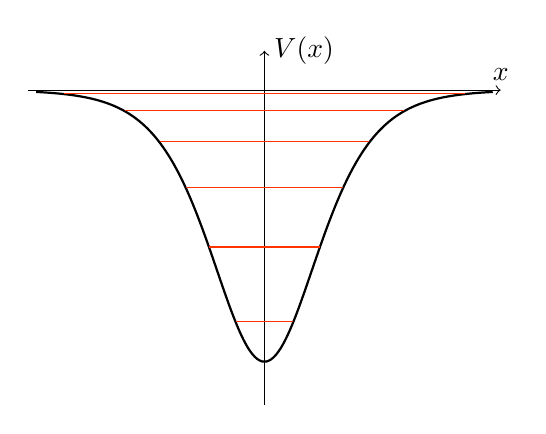
\begin{tikzpicture}
            \draw[->] (-3,0)--(3,0)node[above]{\(x\)};
            \draw[->] (0,-4)--(0,0.5)node[right]{\(V(x)\)};
            \draw[domain=-2.9:2.9, smooth, variable=\x,samples=100,thick] plot ({\x}, {-3.45*(4/(2.718^(1.1*\x)+2.718^(-1.1*\x))^2)});
            \draw[red!80!yellow](-0.36,-2.934)--(0.36,-2.934);
            \draw[red!80!yellow](-0.7,-1.993)--(0.7,-1.993);
            \draw[red!80!yellow](-1,-1.233)--(1,-1.233);
            \draw[red!80!yellow](-1.33,-0.655)--(1.33,-0.655);
            \draw[red!80!yellow](-1.77,-0.258)--(1.77,-0.258);
            \draw[red!80!yellow](-2.55,-0.043)--(2.55,-0.043);
        \end{tikzpicture}
        \caption{The P\"{o}schl--Teller potential \(V(x)=-V_0\sech^2(\kappa x)\) and its energy levels. }
    \end{figure}

    If \(V_0\gg\hbar^2\kappa^2/2m\) then the potential is very deep and contains many bound states. in this regime, we have \(\nu\approx\sqrt{2mV_0/\hbar^2\kappa^2}\gg 1\) and so from (\ref{Poschl_Teller_energy_differences}) we find that a superposition of low-lying states will oscillate with a frequency
    \begin{equation}
        \omega\approx\frac{\hbar\kappa^2}{m}\nu\approx\kappa\sqrt{\frac{2V_0}{m}}\,.
    \end{equation}
    For \(x\ll 1/\kappa\), we may approximate \(-V_0\sech^2(\kappa x)=-V_0+V_0\kappa^2 x^2\), so this frequency is just what we'd expect for the corresponding harmonic oscillator. On the other hand, a superposition of states clustered around \(n=\nu/2\) will oscillate at around half this frequency as neighbouring energy levels in this region are only separated by about half as much.

    If we include a wider range of states in our initial superposition, then we'll instead find a sequence of terms
    \begin{align}
        \expval{X}{\psi,t}=\notag\\
        \dots&+c_{n-1}^*c_n\ee^{\ii (E_{n-1}-E_n)t/\hbar}\mel{n-1}{X}{n}+c_{n+1}^*c_n\ee^{\ii (E_{n+1}-E_n)t/\hbar}\mel{n+1}{X}{n}\notag\\
        &+c_{n+3}^*c_n\ee^{\ii (E_{n+3}-E_n)t/\hbar}\mel{n+3}{X}{n}+\dots\notag\\
        +\dots&+c_n^*c_{n+1}\ee^{\ii (E_n-E_{n+1}t/\hbar)}\mel{n}{X}{n+1}+\dots\,.\label{anharmonic_potential_motion}
    \end{align}
    The potential is symmetric, so we again have \(\mel{n+2k}{X}{n}=0\) by parity, but this is no longer a harmonic potential, so we do not generally expect \(\mel{x+2k+1}{X}{n}=0\).  Let's define a frequency \(\Omega=(E_{n_\text{cl}+1}-E_{n_\text{cl}})\), where \(n_{\text{cl}}\gg 1\). Provided the \(c_n\)'s are clustered around this large central value \(n=n_{\text{cl}}\) sufficiently tightly that the difference between adjacent energy levels is roughly constant over the range of \(n\) for which the \(c_n\) are appreciable, then, to reasonable accuracy, all the terms that contribute to (\ref{anharmonic_potential_motion}) oscillate with frequencies that are integer multiples of \(\Omega_{n_{\text{cl}}}\). Thus the motion will be periodic, but anharmonic, just as we expect classically.

    If we release the anharmonic oscillator from some large extension \(x_0\), then initially the wavefunction will be a superposition of many energy levels, with coefficients that ensure \(\braket{x}{\psi}=\sum_n c_n\braket{x}{n}\) is sharply peaked around \(x_0\). At time \(t\), this state will evolve to
    \begin{equation}
        \ket{\psi,t}=\ee^{-\ii E_{n_\text{cl}}t/\hbar}\sum_{n}c_n \ee^{\ii (E_{b_\text{cl}}-E_n)t/\hbar}\ket{n}\,.
    \end{equation}
    Since the separation between energy levels varies, the frequencies appearing in this sum are not all integer multiples of any \(\Omega_N\). Consequently, after a time of order \(2\pi/\Omega_N\), most terms in the sum will have not quite returned to their original values, so the wavefunction at \(t=2\pi/\Omega\) will be less sharply peaked around \(X\). With each subsequent passing of time \(2\pi/\Omega_N\), the wavefunction will become more and more diffusely spread. Classically, if we release an oscillator with a rather uncertain value for its energy, then for a pure harmonic oscillator we always know where to find the oscillator at later times, since it's period is independent of the energy. However, for an anharmonic oscillator, the period depends on the energy, so after a long time our oscillator is equally likely to be located anywhere.

    \newpage
    \section{Transformations and Symmetries}
    While classical physics is firmly rooted in space-time, quantum mechanics takes place in  the more abstract Hilbert space. Actions such as translations or rotations around a given origin have a straightforward space-time interpretation, but how can these affect a quantum particle living in Hilbert space?

    In this chapter, we'll return to the general formalism of quantum mechanics. We'll understand how transformations such as spatial translations or rotations affect states in Hilbert space, linking together the world of quantum mechanics with our familiar experience in ``normal'' space \(\RR^3\). In so doing, we'll obtain a deeper appreciation of the origin of many of the most common commutation relations, including most of the ones you're familiar with from IB. We'll also understand why the momentum operator is \(P=-\ii\hbar\partial/\partial x\), a fact which probably seemed rather mysterious in IB Quantum Mechanics.

    \subsection{Transformations of States and Operations}
    If we apply a transformation such as a translation or rotation to our physical system, we'd expect states to be different before and after the transformation. For example, if a particle is prepared in a state \(\ket{\psi}\) that is strongly peaked around the origin \(\vb{0}\in\RR^3\) and we translate our system through a vector \(\vb{a}\), after this transformation we should expect to find our particle in a new state \(\ket{\psi'}\) whose wavefunction is strongly peaked around \(\vb{x}=\vb{a}\). This suggests that the effect of any given spatial transformation should be represented on Hilbert space by a linear operator
    \begin{align}
        U:\hb&\longrightarrow\hb\notag\\
        \ket{\psi}&\longmapsto U\ket{\psi}=\ket{\psi'}\,,
    \end{align}
    where the operator depends on the specific type of transformation.

    Whatever state we start with, after applying the transformation, we still expect to find it somewhere in space. Thus, properly normalised states should remain so after applying \(U\), or in other words
    \begin{equation}\label{transformation_preserve_norm_condition}
        1=\braket{\psi}{\psi}=\braket{\psi'}{\psi'}=\expval{U^\dagger U}{\psi}
    \end{equation}
    for all \(\ket{\psi}\in\hb\). We'll now show that the requirement that \(Y\) preserves the norm of our state fixes it to be a \textit{unitary} operator\footnote{Because physical states are represented by rays in \(\hb\), rather than actual vectors, there is one other possibility, transformations may be represented by operators that are both \textit{anti-linear}, in the sense that \(U(c_1\ket{\psi_1}+c_2\ket{\psi_2})=c_1^*U\ket{\psi_1}+c_2^*U\ket{\psi_2}\), and \textit{anti-unitary}, meaning that \(\mel{\chi}{U^\dagger U}{\phi}=\braket{\phi}{\chi}=\braket{\chi}{\phi}^*\) for all \(\ket{\phi},\phi{\chi}\in\hb\). Such anti-unitary operators turn out to be related to reversing the direction of time; we will not discuss them further in this course. Wigner showed that all transformations are represented by either linear, unitary operators or anti-linear, anti-unitary ones}. The required trick is sometimes called the \textit{polarisation identity}. We first write \(\ket{\psi}\) as \(\ket{\psi}=\ket{\phi}+\lambda\ket{\chi}\) for some \(\ket{\phi},\ket{\chi}\in\hb\) and some \(\lambda\in\CC\). Equation (\ref{transformation_preserve_norm_condition}) becomes
    \begin{align}
        \braket{\phi}{\phi}+\lambda^*\braket{\chi}{\phi}+\lambda&\braket{\phi}{\chi}+\abs{\lambda}^2\braket{\chi}{\chi}\notag\\
        &=\expval{U^\dagger U}{\phi}+\lambda^*\mel{\chi}{U^\dagger U}{\phi}+\lambda\mel{\phi}{U^\dagger U}{\chi}+\abs{\lambda}^2\expval{U^\dagger U}{\chi}\,.
    \end{align}
    By assumption, \(\expval{U^\dagger U}{\phi}=\braket{\phi}{\phi}\) and \(\expval{U^\dagger U}{\chi}=\braket{\chi}{\chi}\), so this simplifies to
    \begin{equation}\label{polarisation_identity}
        \lambda\left(\braket{\phi}{\chi}-\mel{\phi}{U^\dagger U}{\chi}\right)=\lambda^*\left(\mel{\chi}{U^\dagger U}{\phi}-\braket{\chi}{\phi}\right)\,.
    \end{equation}
    In order for this to hold for every \(\ket{\psi}\in\hb\), it must continue to hold as we vary \(\lambda\). In particular, as the phase of \(\lambda\) varies, the only way for (\ref{polarisation_identity}) to be satisfied is if
    \begin{equation}
        \braket{\phi}{\chi}=\mel{\phi}{U^\dagger U}{\chi}\,.
    \end{equation}
    Finally, for this hold for arbitrary states \(\ket{\phi}\) and \(\ket{\psi}\) we must have \(U^\dagger U=\Id\). Multiplying through on the right by \(U^{-1}\) shows that
    \begin{equation}\label{unitary_transformation}
        U^\dagger=U^{-1}\,,
    \end{equation}
    which says that the adjoint of \(U\) is equal to its inverse. Operators with these properties are said to be \textit{unitary}\footnote{Note that unitary operators are certainly bounded, and in fact have unit norm in the operator topology.}.

    There's one further condition on our operator \(U\). Transformations of space such as translations and rotations form a \textit{group}. For example, the composition of two rotations is again a rotation, the trivial rotation is the identity, and the inverse of a rotation is a rotation of the same amount around the same axis, but in the opposite direction. Let's suppose that our spatial transformations form a group \(G\). To reflect this group structure, our operators should\footnote{This statement is not quite accurate --- there's an important refinement that we'll return to later in the course.} provide a \textit{homomorphism} from group \(G\) to the group of unitary operators in the sense that, for all \(g_1,g_2\in G\),
    \begin{equation}\label{homomorphism}
        U(g_2)\circ U(g_1)=U(g_2\cdot g_1)\quad\text{and}\quad U(1_G)=1_\hb\,,
    \end{equation}
    where \(\cdot\) denotes the group multiplication in \(G\) and \(\circ\) denotes the composition of linear operators acting on \(\hb\). We'll typically suppress these composition symbols from now on. Note that if \(U_1\) and \(U_2\) are such unitary operators, then \((U_2U_1)^{-1}=U_1^{-1}U_2^{-1}=U_1^\dagger U_2^\dagger=(U_2 U_1)^\dagger\) and so the composite operator \(U_2U_1\) is also unitary. Note also that the identity operator \(1_\hb\) is trivially unitary.

    A particularly important class of transformations are those that depend smoothly on some parameter \(\theta\). For example, we can smoothly vary both the axis about which and the angle through which we rotate, or the magnitude and direction of a translation vector. If \(\theta=0\) is trivial transformation, represented on \(\hb\) by the identity operator, then for infinitesimal transformation of \(\delta\theta\), we have
    \begin{equation}\label{infinitesimal_unitary_transformation}
        U(\delta\theta)=1-\ii\delta\theta T+O(\delta\theta^2)\,,
    \end{equation}
    where \(T\) is some operator that is independent of \(\theta\). The factor \(-\ii\) in this equation is just a convention for later convenience. \(T\) is called the \textit{generator} of the transformation. For such infinitesimal transformations, the condition of unitarity of \(U\) (\ref{unitary_transformation}) becomes
    \begin{equation}
        1+\ii\delta\theta T^\dagger+O(\delta\theta^2)=1+\ii\delta\theta T+O(\delta\theta^2)\,,
    \end{equation}
    which, to first order in \(\delta\theta\), gives
    \begin{equation}
        T=T^\dagger\,.
    \end{equation}
    Thus the generator \(T\) is Hermitian and hence a good candidate for an observable quantity. A finite transformation can be generated by repeatedly performing an infinitesimal one. Specifically, if we set \(\delta\theta=\theta/N\) and transform \(N\) times with \(U(\delta\theta)\), then in the limit \(N\to\infty\) we have
    \begin{equation}
        U(\theta)=\lim_{N\to\infty}\left(1-\ii\frac{\theta}{N}T\right)^N=\ee^{-\ii \theta T}\,,
    \end{equation}
    where the exponential of an operator may be defined by (\ref{function_of_operator}), or equivalently by its power series expansion. This form of the unitary operator \(U(\theta)\) is especially useful when states are expressed in terms of the basis of eigenstates of the Hermitian generator \(T\).

    We obtain an important equation by using (\ref{infinitesimal_unitary_transformation}) to evaluate \(\ket{\psi'}=U(\delta\theta)\ket{\psi}\). Subtracting \(\ket{\psi}\) from both sides and dividing through by \(\delta\theta\), in the limit \(\delta\theta\to 0\) we obtain
    \begin{equation}
        \ii\pdv{\ket{\psi}}{\theta}=T\ket{\psi}\,.
    \end{equation}
    There is no assumption here that the wavefunction \(\psi(\vb{x})=\braket{\vb{x}}{\psi}\) should be differentiable as a function of space. We merely say that as our transformation varies smoothly away from the identity, so too does the state \(\ket{\psi}\) vary smoothly inside \(\hb\). The rate at which \(\ket{\psi}\) varies is governed by the generator.

    Having described how transformations act on states in \(\hb\), we should now understand how they act on operators. Suppose \(A\) is some operator whose matrix elements we are interested in. If our transformation maps \(\ket{\psi}\to\ket{\psi'}\), then the expectation value of \(A\) will be mapped as
    \begin{equation}
        \expval{A}{\psi}\longmapsto\expval{A}{\psi'}=\expval{U^\dagger(\theta) AU(\theta)}{\psi}\,.
    \end{equation}
    Consequently, we can find the expectation value \(A\) will take after the transformation by working with the original states, but instead we can also transform the operator as
    \begin{equation}\label{transformed_operator}
        A\longmapsto A'= U^\dagger(\theta)AU(\theta)=U^{-1}(\theta)AU(\theta)\,,
    \end{equation}
    using the fact that \(U\) is unitary. This is known as a \textit{similarity transform}. Note that
    \begin{equation}
        [A',B']=[U^{-1}AU,U^{-1}BU]=U^{-1}[A,B]U\,,
    \end{equation}
    so the commutator of two similarity transforms is the similarity transform of the commutator. Also, similarity transforms do not change the spectrum of any operator: if \(\ket{\psi}\) is an eigenstate of \(A\) with eigenvalue \(a\), then \(U^{-1}\ket{\psi}\) is an eigenstate of \(A'\) with the same eigenvalue.

    Finally, for an infinitesimal transformation, we have
    \begin{equation}
        U^\dagger(\delta\theta)AU(\delta\theta)=A+\ii\delta\theta[T,A]+O(\delta\theta^2)\,,
    \end{equation}
    so \(\delta A=\ii\delta\theta[T,A]\). Thus, while the rate of change of states themselves is given by the action of the generator, the rate of change of operators under a transformation is determined by the commutator of the generator with the operator. We'll see that most of the commutation relations we meet in quantum mechanics (and certainly all the familiar ones) arise this way. Furthermore, because Hermitian operators represent observable quantities with which we are familiar, in practice it's often easier to understand how a transformation should act on an operator, rather than on the more abstract notion of a state in Hilbert space.

    The above discussion has been rather abstract. Let's ground it by looking at a few of the most important examples of transformations and their corresponding generators.

    \subsection{Translations}
    When we move an object around, we expect to find it in a new place. Specifically, suppose \(\expval{\vb{X}}{\psi}=\vb{x}_0\) for some normalised state \(\ket{\psi}\). Since \(\vb{x}_0\) just labels a spatial point, it must behave under translations and rotations like any vector. Thus, after the translation we expect our object to be described by a new state \(\ket{\psi'}\) with \(\expval{\vb{X}}{\psi'}=\vb{x}_0+\vb{a}\). The general theory of the previous section asserts that this translation is represented on Hilbert space by a unitary operator\footnote{Strictly, we should label this as \(U_\text{trans}(\vb{a})\) to emphasise that it is the unitary operator generating translations, as opposed to anything else we might associate to \(\vb{a}\). We typically drop such additional labels. Exactly which unitary operator we're talking about should hopefully be clear from the context.} \(U(\vb{a})\) so that \(\ket{\psi'}=U(\vb{a})\ket{\psi}\). Therefore we can write the expected location of the translated state as
    \begin{equation}
        \expval{\vb{X}}{\psi'}=\expval{\vb{X}}{\psi}+\vb{a}=\expval{(\vb{X}+1_\hb\vb{a})}{\psi}
    \end{equation}
    where \(1_\hb\) represents the identity operator on \(\hb\). We'll often drop the identity operator where it's unambiguous. Since this is true for any state \(\ket{\psi}\), the transformed operator may be expressed as
    \begin{equation}\label{transformed_translation_operator}
        U^{-1}(\vb{a})\vb{X}U(\vb{a})=\vb{X}+\vb{a}1_\hb
    \end{equation}
    by (\ref{transformed_operator}). Let's be clear what this equation means. In this course, we're interested in quantum mechanics on \(\RR^3\), so the position operator \(\vb{X}:\hb\to\hb\) is really a collection of three operators corresponding to the three coordinates of \(\RR^3\). Taking the standard Cartesian basis of \(\RR^3\), in more detail (\ref{transformed_translation_operator}) says
    \begin{equation}
        \begin{pmatrix}
        U^{-1}(\vb{a})XU(\vb{a})\\
        U^{-1}(\vb{a})YU(\vb{a})\\
        U^{-1}(\vb{a})ZU(\vb{a})
    \end{pmatrix}=\begin{pmatrix}
        X+a_x1_\hb\\
        Y+a_y1_\hb\\
        Z+a_z1_\hb
    \end{pmatrix}\,.
    \end{equation}
    In other words, conjugating the \(X\) (component) operator by \(U(\vb{a})\) gives a new operator \(U^{-1}(\vb{a})XU(\vb{a}):\hb\to\hb\) that we identify with \(X+a_x\), and similarly for \(Y\) and \(Z\). If \(U(\vb{a})\) acted on the position operator in any other way, it could not represent a translation, so equation (\ref{transformed_translation_operator}) may be taken as the defining property of the translation operator, distinguishing it from other unitary transformations.

    For an infinitesimal translation \(\delta\vb{a}\), equation (\ref{infinitesimal_unitary_transformation}) states that the translation operator can be written as\footnote{Here, \(\delta\vb{a}\vdot\vb{P}=\sum_i\delta a_iP_i\) involves the standard dot product in \(\RR^3\). Note that the result is still an operator on \(\hb\), a linear combination of the operators \(\vb{P}\).}
    \begin{equation}\label{infinitesimal_translation_operator}
        U(\delta\vb{a})=1-\frac{\ii}{\hbar}\delta\vb{a}\vdot\vb{P}+O(\delta\vb{a}^2)\,,
    \end{equation}
    where \(\vb{P}\) is Hermitian. I've named this operator \(\vb{P}\), so I'm not going to be able to fool any of you that it will turn out to be anything other than the momentum operator. But that's not how I want you to think of it yet. By definition, \(\vb{P}/\hbar\) is the generator of infinitesimal
    translations.

    The translation generator \(\vb{P}/\hbar\) must have units \(1/(\text{length})\) so that it makes sense to add the second term of (\ref{infinitesimal_translation_operator}) to the first. Because we've included a factor of \(\hbar\), our \(\vb{P}\) must have dimensions of (\(\text{mass}\times\text{velocity}\)). In fact, this is just a convention. We could choose to measure masses in units of \(1/(\text{length}\times\text{velocity})\), using \(\hbar\) as a conversion factor for our units. In relativity, the speed of light \(c\) provides a further natural conversion factor between lengths and times, so in units of \(\hbar/c\), masses are equivalent to inverse lengths. In natural units, we work with length and time scales adapted to Nature rather than our civilisation, so we set \(\hbar=1\) and \(c=1\). In these units, the translation generator is precisely \(\vb{P}\). Incidentally, you may be worried about setting \(\hbar=1\) when it is such a ``small'' number; \(\hbar\approx 1.0547\times 10^{-34}\unit{J}\unit{s}\unit{rad}^{-1}\). But this is quite wrong. Every atom in the Universe knows that \(\hbar\) is not at all small or insignificant. It only appears small when measured in units such as Joules and seconds that are relevant for steam engines and pocketwatches. The real, deep question is not why \(\hbar\) appears small, but why humans are so big.

    Plugging (\ref{infinitesimal_translation_operator}) into the defining equation (\ref{transformed_translation_operator}) for the translation operator we find
    \begin{equation}
        \frac{\ii}{\hbar}[\delta\vb{a}\vdot\vb{P},\vb{X}]=\delta\vb{a}\,,
    \end{equation}
    and since this holds for any infinitesimal translation,
    \begin{equation}
        [X_i,P_j]=\ii\hbar\delta_{ij}\,.
    \end{equation}
    These, as I'm sure you recognise, are the fundamental commutation relations of quantum mechanics. I'm prepared to bet that the first time you met them (and perhaps even up until now) you thought they were a weird and mysterious feature of quantum mechanics. Here they're revealed as little more than common sense: asking where you are and then translating is not the same as first translating and then asking where you are. What is weird and quantum about this equation is not that \(\vb{X}\) and \(\vb{P}\) don't commute, but the fact that they are operators acting on a Hilbert space.

    By repeatedly performing the same infinitesimal translation, we can write
    \begin{equation}
        U(\vb{a})=\exp\left(-\frac{\ii}{\hbar}\vb{a}\vdot\vb{P}\right)
    \end{equation}
    for a translation through the finite vector \(\vb{a}\). Since \(U(\vb{a})\) provides a homomorphism of this group of translations to the group of linear operators on \(\hb\), we have
    \begin{equation}
        U(\vb{b})U(\vb{a})=U(\vb{b}+\vb{a})=U(\vb{a}+\vb{b})=U(\vb{a})U(\vb{b})\,,
    \end{equation}
    where in the second equality we used the fact that \(\vb{a}+\vb{b}=\vb{b}+\vb{a}\), stating that the order in which we perform two translations doesn't matter\footnote{Here this is of course the statement that the group of spatial translations is \((\RR^3,+)\), where the group operation ``+'' is commutative. Groups for which the group operation is commutative are often called \textit{Abelian}.}. Using (\ref{infinitesimal_translation_operator}) to expand the far left and far right of this equation to lowest non-trivial order in \(a_ib_j\) shows that the generators \(\vb{P}\) obey
    \begin{equation}
        [P_i,P_j]=0\text{ for all }i,j\,,
    \end{equation}
    and so they commute with each other. Again, the fundamental meaning of this equation is simply that translations form an Abelian group --- the order of translations doesn't matter. It only says anything about our ability to simultaneously know all three components of a particle's momentum once we identify \(\vb{P}\) as corresponding to momentum, which we haven't yet done.

    Now let's think about what the translation operator does to states. Let \(\ket{\vb{x}}\) represent an eigenstate of the position operator with eigenvalue \(\vb{x}\), so that \(\vb{X}\ket{\vb{x}}=\vb{x}\ket{\vb{x}}\), with normalisation condition
    \begin{equation}
        \braket{\vb{x}'}{\vb{x}}=\delta(\vb{x}'-\vb{x})
    \end{equation}
    as usual for continuum states\footnote{Technically, \(\ket{\vb{x}}\) is a non-normalisable state, which really means it doesn't live in the Hilbert space \(L^2(\RR,\dd[3]{\vb{x}})\). This is related to the fact that the position operator \(\vb{X}\) is unbounded --- there is no constant \(M\) such that \(\norm{\vb{X}\ket{\psi}}\le M\norm{\ket{\psi}}\) for all \(\ket{\psi}\in\hb\). Naively, this means that ``the eigenvalue of \(\vb{X}\) can be arbitrarily large'', which is physically reasonable since our particle may be located very far away. However, in general, unbounded operators do not have any eigenstate in \(\hb\), so do not really have eigenvalues. The distinction between bounded and unbounded operators is tremendously important in functional analysis, but will not play a role in this course.}. This state represents a particle which is definitely located at \(\vb{x}\in\RR^3\). Applying the translation operator,
    \begin{equation}
        \vb{X}(U(\vb{a})\ket{\vb{x}})=([\vb{X},U(\vb{a})]+U(\vb{a})\vb{X})\ket{\vb{x}}\,.
    \end{equation}
    We can evaluate the commutator by multiplying (\ref{transformed_translation_operator}) through by \(U(\vb{a})\) on the left, finding \([\vb{X},U(\vb{a})]=U(\vb{a})\vb{a}\). Since \(\vb{a}\) is just a constant vector (not an operator on \(\hb\)) it commutes with the translation operator, so
    \begin{equation}
        \vb{X}(U(\vb{a})\ket{\vb{x}})=(\vb{x}+\vb{a})(U(\vb{a})\ket{\vb{x}})\,.
    \end{equation}
    As anticipated, our new state \(U(\vb{a})\ket{\vb{x}}\) is certainly located at \(\vb{x}+\vb{a}\). Consequently, \(U(\vb{a})\ket{\vb{x}}\) must be proportional to the state \(\ket{\vb{x}+\vb{a}}\), the normalised state that is definitely located at \(\vb{x}+\vb{a}\). Setting \(U(\vb{a})\ket{\vb{x}}=c\ket{\vb{x}+\vb{a}}\) for some \(c\in\CC\) and taking the inner product with another position eigenstate \(\ket{\vb{x}'}\), we have
    \begin{align}
        c\delta(\vb{x}'-\vb{x}-\vb{a})&=c\braket{\vb{x}'}{\vb{x}+\vb{a}}=\mel{\vb{x}'}{U(\vb{a})}{\vb{x}}=\left(U^{-1}(\vb{a})\ket{\vb{x'}}\right)^\dagger\ket{\vb{x}}\notag\\
        &=\left(\frac{1}{c}\ket{\vb{x}'-\vb{a}}\right)^\dagger\ket{\vb{x}}=\frac{1}{c^*}\delta(\vb{x}'-\vb{a}-\vb{x})\,,
    \end{align}
    where we used the fact that \(U(\vb{a})\) is unitary. Comparing both sides shows that \(\abs{c}^2=1\), so \(c\) is a pure phase and without loss of generality we can set \(c=1\).

    Now suppose we consider translating an arbitrary state \(\ket{\psi}\). The position space wavefunction of this state is simply its coefficient
    \begin{equation}
        \psi(\vb{x})=\braket{\vb{x}}{\psi}
    \end{equation}
    in the position basis. Thus the wavefunction \(\psi_{\text{trans}}(\vb{x})\) of the translated state \(\ket{\psi_{\text{trans}}}=U(\vb{a})\ket{\psi}\) is
    \begin{align}
        \psi_{\text{trans}}(\vb{x})=\braket{\vb{x}}{\psi_\text{trans}}&=\mel{\vb{x}}{U(\vb{a})}{\psi}=(U^{-1}(\vb{a})\ket{\vb{x}})\ket{\psi}\notag\\
        &=\braket{\vb{x}-\vb{a}}{\psi}=\psi(\vb{x}-\vb{a})\,.
    \end{align}
    This says that the wavefunction of the translated state takes the same value at \(\vb{x}\) as the original wavefunction took at \(\vb{x}-\vb{a}\). This is completely natural as we've translated our state through \(\vb{a}\).

    In particular, for an infinitesimal translation \(\delta\vb{a}\), on the one hand we can Taylor expand the translated wavefunction to find\footnote{At least if the wavefunction is sufficiently smooth}
    \begin{equation}
        \psi_\text{trans}(\vb{x})-\psi(\vb{x})=-\delta\vb{a}\vdot\grad{\psi(\vb{x})}\,,
    \end{equation}
    while on the other hand we expand the operator \(U(\delta\vb{a})\) to find
    \begin{equation}
        \psi_\text{trans}(\vb{x})-\psi(\vb{x})=\mel{\vb{x}}{1-\frac{\ii}{\hbar}\delta\vb{a}\vdot\vb{P}}{\psi}-\braket{\vb{x}}{\psi}=-\frac{\ii}{\hbar}\delta\vb{a}\vdot\mel{\vb{x}}{\vb{P}}{\psi}
    \end{equation}
    using (\ref{infinitesimal_translation_operator}) to the lowest order in \(\delta\vb{a}\). Consequently, for any state \(\ket{\psi}\) the momentum operator \(\vb{P}\) acts in the position representation as
    \begin{equation}\label{momentum_operator_position_representation}
        \mel{\vb{x}}{\vb{P}}{\psi}=-\ii\hbar\grad{\psi(\vb{x})}\,.
    \end{equation}
    This is just what you would have said in IB Quantum Mechanics last year, here derived from the point of view of the effect a translation of \(\RR^3\) has on states in Hilbert space.

    As a special case, let's apply this argument to the state \(\ket{\vb{p}}\) that obeys\footnote{As with the position operator, the momentum operator \(\vb{P}\) is unbounded, so the ``momentum eigenstates'' \(\ket{\vb{p}}\) are necessarily non-normalisable, as we'll soon see explicitly.} \(\vb{P}\ket{\vb{p}}=\vb{p}\ket{\vb{p}}\), representing a particle whose momentum is certainly \(\vb{p}\). In this case the above argument becomes
    \begin{align}
        \psi_{\vb{p}}(\vb{x}-\vb{a})&=\braket{\vb{x}-\vb{a}}{\vb{p}}=\mel{\vb{x}}{U(\vb{a})}{\vb{p}}=\mel{\vb{x}}{\ee^{-\ii \vb{a}\vdot\vb{P}/\hbar}}{\vb{p}}\notag\\
        &=\ee^{-\ii \vb{a}\vdot\vb{p}/\hbar}\braket{\vb{x}}{\vb{p}}=\ee^{-\ii \vb{a}\vdot\vb{p}/\hbar}\psi_{\vb{p}}(\vb{x})\,.
    \end{align}
    Comparing the first and last expression, we deduce that the position space wavefunction of a momentum eigenstate must take the form
    \begin{equation}
        \psi_{\vb{p}}(\vb{x})=C\ee^{\ii \vb{p}\vdot\vb{x}/\hbar}
    \end{equation}
    for some \(\vb{x}\)-independent factor \(C\in\CC\). It's convenient to choose \(C\) to be \((2\pi\hbar)^{-3/2}\) since in this case we have
    \begin{align}
        \braket{\vb{p}'}{\vb{p}}&=\int\dd[3]{\vb{y}}\dd[3]{\vb{x}}\braket{\vb{p}'}{\vb{y}}\braket{\vb{y}}{\vb{x}}\braket{\vb{x}}{\vb{p}}=\int\dd[3]{\vb{x}}\dd[3]{\vb{y}}\frac{1}{(2\pi\hbar)^3}\ee^{-\ii \vb{p}'\vdot\vb{y}/\hbar}\delta(\vb{y}-\vb{x})\ee^{\ii \vb{p}\vdot\vb{x}/\hbar}\notag\\
        &=\int\dd[3]{\vb{x}}\frac{1}{(2\pi\hbar)^3}\ee^{-\ii (\vb{p}'-\vb{p})\vdot\vb{x}/\hbar}=\delta(\vb{p}'-\vb{p})\,,
    \end{align}
    so that the momentum eigenstates are normalised in the same way as the position eigenstates (and in the same way as for any continuum states). Again, the form
    \begin{equation}
        \psi_{\vb{p}}(\vb{x})=\frac{1}{(2\pi\hbar)^{3/2}}\ee^{\ii \vb{p}\vdot\vb{x}/\hbar}
    \end{equation}
    of the wavefunction for momentum eigenstates is familiar, but here we've derived it from first principles rather than using the position space representation (\ref{momentum_operator_position_representation}) of the momentum operator. (We assumed this result earlier when showing that the position and momentum space wavefunctions are each other's Fourier transformations.) Note also that \(\abs{\psi_{\vb{p}}(\vb{x})}^2=1/(2\pi\hbar)^3\), so \(\int_{\RR^3}\dd[3]{\vb{x}}\abs{\psi_{\vb{p}}(\vb{x})}^2\) diverges, Like position eigenvalues, momentum eigenstates are also non-normalisable.

    \subsection{Rotations}
    We now consider the effect rotating \(\RR^3\) has on a quantum state \(\ket{\psi}\in\hb\). For a vector \(\vb{v}\in\RR^3\), a rotation anticlockwise around the axis \(\vu{\alpha}\) by an amount \(\abs{\vb{\alpha}}\) is a linear transformation
    \begin{align}
        \mathsf{R}(\vb{\alpha}):\RR^3&\longrightarrow\RR^3\notag\\
        \vb{v}&\longmapsto\vb{v}'=\mathsf{R}(\vb{\alpha})\vb{v}
    \end{align}
    that obeys
    \begin{equation}\label{rotation_matrix_conditions}
        \vb{v}'\vdot\vb{v}'=\vb{v}\vdot\vb{v}\quad\text{and}\quad\det(\mathsf{R}(\vb{\alpha}))=+1\,.
    \end{equation}
    The first of these conditions says that rotations preserve lengths, and implies that \(\mathsf{R}(\vb{\alpha})\) must be an \textit{orthogonal} transformation. The second ensures that \(\mathsf{R}(\vb{\alpha})\) preserves the orientation. For infinitesimal rotations, \cref{Fig:infinitesimal_rotation} shows that
    \begin{equation}\label{infinitesimal_vector_rotation}
        \vb{v}'=\vb{v}+\delta\vb{\alpha}\cross\vb{v}+O(\delta\vb{\alpha}^2)\,.
    \end{equation}
    Note that this obeys (\ref{rotation_matrix_conditions}). Given two orthogonal transformations \(\mathsf{R}(\vb{\alpha})\) and \(\mathsf{R}(\vb{\beta})\), the composite \(\mathsf{R}(\vb{\beta})\mathsf{R}(\vb{\alpha})\) is again an orthogonal transformation with unit determinant. Spatial rotations form a group, known as \(\SO(3)\), with the identity being the trivial rotation and the inverse of \(\mathsf{R}(\vb{\alpha})\) being a rotation of the same amount around the same axis \(\vb{\alpha}\), but now clockwise. However, in general \(\mathsf{R}(\vb{\beta})\mathsf{R}(\vb{\alpha})=\mathsf{R}(\vb{\alpha})\mathsf{R}(\vb{\beta})\), so the order in which we apply rotations is important and the rotation is \textit{non-Abelian}.

    \begin{figure}
        \centering
        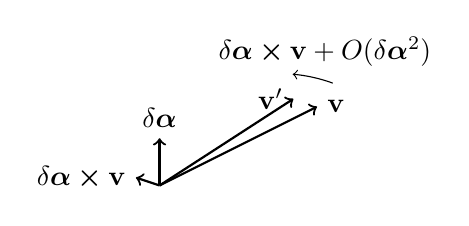
\begin{tikzpicture}
            \draw[->,thick] (0,0)--(0,0.6)node[above]{\(\delta\vb{\alpha}\)};
            \draw[->,thick] (0,0)--(2,1)node[right]{\(\vb{v}\)};
            \draw[->,thick] (0,0)--(-0.3,0.1)node[left]{\(\delta\vb{\alpha}\cross\vb{v}\)};
            \draw[->,thick] (0,0)--(1.7,1.1)node[left]{\(\vb{v}'\)};
            \draw [->] (2.2,1.3) arc (70:85:2);
            \node at (2.1,1.7) {\(\delta\vb{\alpha}\cross\vb{v}+O(\delta\vb{\alpha}^2)\)};
        \end{tikzpicture}
        \caption{An infinitesimal rotation transforms \(\vb{v}\mapsto\vb{v}+\delta\vb{\alpha}\cross\vb{v}\).}
        \label{Fig:infinitesimal_rotation}
    \end{figure}

    As for any group of transformations, in quantum mechanics the group of rotations is represented on \(\hb\) by unitary operators. We denote the unitary operator corresponding to \(\mathsf{R}(\vb{\alpha})\) as \(U(\vb{\alpha})\). \(U(\vb{\alpha})\) acts on the position operator as
    \begin{equation}\label{rotation_operator}
        U^{-1}(\vb{\alpha})\vb{X}U(\vb{\alpha})=\mathsf{R}(\vb{\alpha})\vb{X}\,,
    \end{equation}
    where the left-hand side involves composition of operators in \(\hb\), while the right-hand side is the usual action of a rotation on the three components of \(\vb{X}\). For example, if \(\vb{\alpha}=\alpha\hat{\vb{z}}\) so that the rotation is around the \(z\)-axis in \(\RR^3\), then in more detail (\ref{rotation_operator}) says
    \begin{equation}
        \begin{pmatrix}
        U^{-1}(\vb{\alpha})XU(\vb{\alpha})\\
        U^{-1}(\vb{\alpha})YU(\vb{\alpha})\\
        U^{-1}(\vb{\alpha})ZU(\vb{\alpha})\\
    \end{pmatrix}=\begin{pmatrix}
        \cos\alpha & -\sin\alpha & 0\\
        \sin\alpha & \cos\alpha & 0\\
        0 & 0 & 1
    \end{pmatrix}\begin{pmatrix}
        X \\ Y \\ Z
    \end{pmatrix}\,.
    \end{equation}
    Thus, conjugating the operator \(X\) by this rotation operator changes it to a new operator \(U^{-1}(\vb{\alpha})XU(\vb{\alpha})\) on Hilbert space, which we identity with the usual linear combination \(X\cos\alpha-Y\sin\alpha\). Again, \(U(\vb{\alpha})\) must act on \(\vb{X}\) this way if it is indeed to correspond to a rotation.

    For an infinitesimal transformation, following (\ref{infinitesimal_unitary_transformation}) we can write
    \begin{equation}\label{infinitesimal_rotation_operator}
        U(\delta\vb{\alpha})=1-\frac{\ii}{\hbar}\delta\vb{\alpha}\vdot\vb{J}+O(\delta\vb{\alpha}^2)
    \end{equation}
    for some Hermitian generators \(\vb{J}/\hbar\). Since angles are dimensionless, \(\vb{J}\), like \(\hbar\), must have dimensions of (\(\text{length}\times\text{momentum}\)). Later we will see that \(\vb{J}\) corresponds to the angular momentum operator, though by definition we have that \(\vb{J}/\hbar\) is the generator of rotations. Using this and (\ref{infinitesimal_vector_rotation}) in (\ref{rotation_operator}) shows that we have
    \begin{equation}
        \frac{\ii}{\hbar}[\delta\vb{\alpha}\vdot\vb{J},\vb{X}]=\delta\vb{\alpha}\cross\vb{X}\,,
    \end{equation}
    and since this is true for any axis of rotation, we have the commutation relations
    \begin{equation}
        [J_i,X_j]=\ii\hbar\sum_{k}\epsilon_{ijk}X_k\,.
    \end{equation}
    These relations are nothing more than the statement that the operator \(\vb{X}\) transforms as a vector under rotations. They are the infinitesimal version of (\ref{rotation_matrix_conditions}) --- they must hold if \(\vb{J}\) is indeed to generate rotations.

    Just as for translations, the mutual commutation relations among the components of \(\vb{J}\) themselves follow from the fact that the \(U(\vb{\alpha})\)'s provide a homomorphism from the group\footnote{Again, later we'll see that this statement needs to be slightly refined.} \(\SO(3)\) of rotations to the space of unitary operators on \(\hb\). However, the non-Abelian nature of the rotation group means we should expect these commutators to be non-trivial in general. Performing two infinitesimal rotations through angles \(\delta\vb{\alpha}\) and \(\delta\vb{\beta}\) for any vector \(\vb{v}\) gives
    \begin{align}
        \mathsf{R}(\delta\vb{\beta})\mathsf{R}(\delta\vb{\alpha})\vb{v}&=\mathsf{R}(\delta\vb{\beta})(\vb{v}+\delta\vb{\alpha}\cross\vb{v})=(\vb{v}+\delta\vb{\alpha}\cross\vb{v})+\delta\vb{\beta}\cross(\vb{v}+\delta\vb{\alpha}\cross\vb{v})\notag\\
        &=\vb{v}+\delta\vb{\alpha}\cross\vb{v}+\delta\vb{\beta}\cross\vb{v}+\delta\vb{\beta}\cross(\delta\vb{\alpha}\cross\vb{v})
    \end{align}
    to the lowest non-trivial order in \(\delta\vb{\alpha}\) and \(\delta\vb{\beta}\). Consequently, the difference between these rotations and the two rotations performed in the opposite order is
    \begin{align}
        [\mathsf{R}(\delta\vb{\beta})\mathsf{R}(\delta\vb{\alpha})-\mathsf{R}(\delta\vb{\alpha})\mathsf{R}(\delta\vb{\beta})]&=\delta\vb{\beta}\cross(\delta\vb{\alpha}\cross\vb{v})-\delta\vb{\alpha}\cross(\delta\vb{\beta}\cross\vb{v})\notag\\
        &=(\delta\vb{\beta}\cross\delta\vb{\alpha})\cross\vb{v}\notag\\
        &=\mathsf{R}(\delta\vb{\beta}\cross\delta\vb{\alpha})\vb{v}-\vb{v}
    \end{align}
    using the standard properties of the vector triple product. The right-hand side again involves a rotation, through \(\delta\vb{\beta}\cross\delta\vb{\alpha}\). Applying the homomorphism \(U\), we obtain
    \begin{equation}
        [U(\delta\vb{\beta}),U(\delta\vb{\alpha})]=U(\delta\vb{\beta}\cross\delta\vb{\alpha})-1_{\hb}
    \end{equation}
    for our operators in Hilbert space. Using (\ref{infinitesimal_rotation_operator}), this is
    \begin{equation}
        -\frac{1}{\hbar^2}[\delta\vb{\beta}\vdot\vb{J},\delta\vb{\alpha}\vdot\vb{J}]=-\frac{\ii}{\hbar}(\delta\vb{\beta}\cross\delta\vb{\alpha})\vdot\vb{J}\,,
    \end{equation}
    and since this must hold for arbitrary successive infinitesimal rotations, we have
    \begin{equation}\label{angular_momentum_commutation}
        [J_i,J_j]=\ii\hbar\sum_k\epsilon_{ijk}J_k
    \end{equation}
    as the commutation relations among the rotation generators.

    Again, there's nothing ``weird'' or ``quantum'' about (\ref{angular_momentum_commutation}), beyond the fact that they involve operators on Hilbert space. In particular, their form just reflects the fact that the order of rotations around different axes matters, and that the difference between the two ordering is itself a rotation around the axis perpendicular the original two. Compared to the relations \([P_i,P_j]=0\), the non-triviality of the commutation relations (\ref{angular_momentum_commutation}) arises purely because \(\SO(3)\) is a non-Abelian group, unlike the group of translations. These non-trivial commutation relations do not prevent us from exponentiating the infinitesimal rotation operator (\ref{infinitesimal_rotation_operator}) to write \(U(\vb{\alpha})=\ee^{-\ii \vb{\alpha}\vdot\vb{J}/\hbar}\) for a finite rotation around a fixed axis \(\vb{\alpha}\), because the exponentiation always involve the same component \(\hat{\vb{\alpha}}\vdot\vb{J}\) of the rotation generator, which certainly commutes with itself.

    The combined group of translations and rotations of Euclidean space \(\RR^3\) is known as the \textit{Euclidean group}, denoted \(\E(3)\) or \(\mathrm{ISO}(3)\). For translations through \(\vb{a}_1\) and \(\vb{a}_2\), and rotations \(\mathsf{R}_1\) and \(\mathsf{R}_2\), \(E_3\) has the group composition law
    \begin{equation}
        (\vb{a}_2,\mathsf{R}_2)\cdot(\vb{a}_1,\mathsf{R}_1)=(\vb{a}_2+\mathsf{R}_2\vb{a}_1,\mathsf{R}_2\mathsf{R}_1)\,,
    \end{equation}
    where we note that the second rotation also acts on the first translation. Clearly, both \(\RR^3\) and \(\SO(3)\) are subgroups of \(\E(3)\), but the fact that the rotations act non-trivially on previous translations means that \(\E(3)\) is the \textit{semi-direct product} \(\E(3)\cong\RR^3\rtimes \SO(3)\). This group composition law shows that rotations and translations do not commute: translating any vector \(\vb{v}\) through \(\vb{a}\) then rotating around \(\hat{\vb{\alpha}}\) gives us \(\mathsf{R}(\vb{\alpha})(\vb{v}+\vb{a})\), whereas first rotating then translating gives \(\vb{a}+\mathsf{R}(\vb{\alpha})\vb{v}\) instead. In particular, for infinitesimal translations and rotations we have
    \begin{equation}
        \mathsf{R}(\delta\vb{\alpha})(\vb{v}+\delta\vb{a})-(\delta\vb{a}+\mathsf{R}(\delta\vb{\alpha})\vb{v})=\delta\vb{\alpha}\cross\delta\vb{a}
    \end{equation}
    independent of \(\vb{v}\). Applying the homomorphism \(U\), in Hilbert space we obtain commutation relations
    \begin{equation}
        [U_R(\delta\vb{\alpha}),U_T(\delta\vb{a})]=U_T(\delta\vb{\alpha}\cross\delta\vb{a})-1\,,
    \end{equation}
    where, for the sake of clarity, we have labelled the translations operator by \(U_T\) and rotation operator by \(U_R\). Equivalently, we have
    \begin{equation}
        [J_i,P_j]=\ii\hbar\sum_k \epsilon_{ijk}P_k
    \end{equation}
    in terms of the rotation and translation generators.

    More generally, and 3-component linear operator \(\vb{V}:\hb\to\hb\) is said to \textit{transform as a vector under rotations} if it obeys \(U^{-1}(\vb{\alpha})\vb{V}U(\vb{\alpha})=\mathsf{R}(\vb{\alpha})\vb{V}\) for any \(\vb{\alpha}\). Depending on its behaviour under parity transformations, which will be discussed in \cref{Chap:Parity}, such a vector \(\vb{V}\) could either be a vector or a pseudovector operator. Just as above, for infinitesimal rotations this implies the commutation relations
    \begin{equation}\label{angular_momentum_vector_commutator}
        [J_i,V_j]=\ii\hbar\sum_k\epsilon_{ijk}V_k
    \end{equation}
    for the components of \(\vb{V}\) and \(\vb{J}\). We see that \(\vb{X},\vb{P}\) and \(\vb{J}\) itself\footnote{This is always true of \(\vb{X}\) and \(\vb{P}\), but turns out to be a three-dimensional coincidence for \(\vb{J}\): the rotation group \(\SO(d)\) of \(\RR^d\) has dimension \(d(d-1)/2\) and the generators are generically represented by antisymmetric matrices \(\mathcal{J}_{ij}\). When \(d=3\), a \(3\times 3\) antisymmetric matrix has \(3\) independent components, so we can equivalently package the \(\mathcal{J}_{ij}\) as vectors through \(J_i=\epsilon_{ijk}\mathcal{J}_{jk}\).} each transform as vectors under rotations. This of course is just what we'd expect for position, momentum and angular momentum in classical mechanics.

    On the other hand, if an operator \(S\) obeys
    \begin{equation}
        U^{-1}(\vb{\alpha})SU(\vb{\alpha})=S
    \end{equation}
    for any \(\vb{\alpha}\), so that it is unchanged by the rotation operator, we say \(S\) \textit{transforms as a scalar under rotations}. Again, depending on its behaviours under parity transformations it could either be a scalar or a pseudoscalar operator. The corresponding infinitesimal version is
    \begin{equation}\label{angular_momentum_scalar_commutation}
        [\vb{J},S]=0\,.
    \end{equation}
    Just as we can form a scalar by taking the Euclidean inner product \(\vb{v}\vdot\vb{w}\) of the two vectors \(\vb{v},\vb{w}\in\RR^3\), we can form scalar operators from Euclidean inner product of two vector operators. Indeed, if \(U^{-1}(\vb{\alpha})\vb{V}U(\vb{\alpha})=\mathsf{R}(\vb{\alpha})\vb{V}\) and similarly for \(\vb{W}\), then
    \begin{align}
        U^{-1}(\vb{\alpha})(\vb{V}\vdot\vb{W})U(\vb{\alpha})&=(U^{-1}(\vb{\alpha})\vb{V}U(\vb{\alpha}))\vdot(U^{-1}(\vb{\alpha})\vb{W}U(\vb{\alpha}))\notag\\
        &=(\mathsf{R}(\vb{\alpha})\vb{V})\vdot(\mathsf{R}(\vb{\alpha})\vb{W})\notag\\
        &=\vb{V}\vdot\vb{W}
    \end{align}
    by the standard rotational invariance of the dot product. As always, we can write this in
    terms of commutators by considering infinitesimal rotations:
    \begin{align}
        \left[J_i,\sum_j V_jW_j\right]&=\sum_j[J_i,V_j]W_j+\sum_jV_j[J_i,W_j]\notag\\
        &=\ii\hbar\sum_{j,k}\epsilon_{ijk}V_kW_j+\ii\hbar\sum_{j,k}V_j\epsilon_{ijk}W_k\notag\\
        &=\ii\hbar\sum_{j,k}\epsilon_{ijk}(-V_jW_k+V_jW_k)=0\,,
    \end{align}
    where in going to the final line we relabelled the dummy indices \(j\leftrightarrow k\) in the first term and used the antisymmetry of \(\epsilon_{ijk}\). Note that our calculations always preserved the order of \(\vb{V}\) and \(\vb{W}\), so our result holds irrespective of whether \(\vb{V}\) and \(\vb{W}\) commute or not.

    An important special case of (\ref{angular_momentum_scalar_commutation}) is to take \(S=\vb{J}^2=\vb{J}\vdot\vb{J}\). The fact that the rotation generators obey the commutation relations
    \begin{equation}
        [J_i,J_j]=\ii\hbar\sum_k\epsilon_{ijk}J_k\quad\text{and}\quad[J_i,\vb{J}^2]=0
    \end{equation}
    means that we cannot find a complete set of simultaneous eigenstates of all of the \(J_i\)'s, but we can find a complete set of simultaneous eigenstates of \(\vb{J}^2\) and any one component of \(\vb{J}\). Looking ahead to our interpretation of \(\vb{J}\) as the angular momentum operator, Born's \(2^{\text{nd}}\) postulate of quantum mechanics tells us that we cannot say a particle has a definite angular momentum vector, but we can know the magnitude of the angular momentum and the amount aligned along any given axis.

    \subsubsection{Translations Around a Circle}
    In IB Quantum Mechanics, we defined the orbital angular momentum operator \(\vb{L}=\vb{X}\cross\vb{P}\) which also has the commutation relations (\ref{angular_momentum_vector_commutator}) with itself and with X and P. We'll understand the relation between \(\vb{J}\) and \(\vb{L}\) later, but it's important to understand that in general \(\vb{J}\ne\vb{L}\). We can understand \(\vb{L}\) from the present perspective as follows.

    When a system is displaced through the vector \(\vb{a}\), its state is transformed by the unitary operator \(U(\vb{a})=\ee^{-\ii \vb{a}\vdot\vb{P}/\hbar}\). We now imagine successively performing \(n\) translations successively through the set of vectors \(\{\vb{a}_1,\vb{a}_2,\dots,\vb{a}_n\}\). Each translation is represented by a unitary operator \(U(\vb{a}_i)\), so the final state will be
    \begin{equation}
        U(\vb{a}_n)\dots U(\vb{a}_1)\ket{\psi}=U(\vb{b})\ket{\psi}\,,
    \end{equation}
    where \(\vb{b}=\vb{a}_1+\dots\vb{a}_n\) is the total displacement vector. Since the net result depends only on the total translation \(\vb{b}\), the change in \(\ket{\psi}\) is independent of the particular path that the system takes. In particular, if the path is closed so that \(\vb{a}_1+\dots+\vb{a}_n=\vb{0}\), then \(\ket{\psi}\) is unchanged.

    Now consider the effect of translating the system around an arc of a circle centred on the origin. We can approximate the circle by an \(N\)-sided regular polygon, with the approximation improving as \(N\to\infty\), so we move around a circle by applying a succession of small translations, each in a slightly different direction. Specifically, if the system initially lies at some location \(\vb{x}\), making an angle \(\alpha\) with some axis \(\vb{n}\), then when move it in the plane normal to \(\vb{n}\) to lie at an angle \(\alpha+\delta\alpha\), we translate it through \(\delta\vb{a}=\delta\alpha\vb{n}\cross\vb{x}\). Thus the associated unitary translation operator obeys
    \begin{equation}
        U^{-1}(\delta\vb{a})\vb{X}U(\delta\vb{a})=\vb{X}+\delta\alpha(\vb{n}\cross\vb{X})\,,
    \end{equation}
    and so can be written as
    \begin{equation}\label{infinitesimal_circular_transformation}
        U(\delta\vb{a})=1-\frac{\ii}{\hbar}\delta\alpha(\vb{n}\cross\vb{X})\vdot\vb{P}+O(\delta\alpha^2)=1-\frac{\ii}{\hbar}\delta\alpha\vb{n}\vdot\vb{L}+O(\delta\alpha^2)\,,
    \end{equation}
    where
    \begin{equation}
        \vb{L}=\vb{X}\cross\vb{P}
    \end{equation}
    is a Hermitian operator. We now see that \(\vb{L}\) is the generator of circular transformations. (\ref{infinitesimal_circular_transformation}) contains only one operator \(\vb{n}\vdot\vb{L}\), so it inevitably commutes with itself and we can exponentiate to find \(U(\vb{a}_{\text{circ}})=\ee^{-\ii \alpha\vb{n}\vdot\vb{L}/\hbar}\) for finite translations around our circle.

    \subsubsection{Spin}
    The commutation relations \([L_i,X_j]\), \([L_i,P_j]\) and \([L_i,L_j]\) of the composite operator \(\vb{L}\) all follow from the more primitive commutation relations \([X_i,P_j]\), \([X_i,X_j]\) and \([P_i,P_j]\). If we're only concerned with these operators, then \(U_{\text{circ}}=\ee^{-\ii \alpha\vb{n}\vdot\vb{L}/\hbar}\) is indistinguishable from the rotation operator \(U(\vb{\alpha})=\ee^{-\ii \vb{\alpha}\vdot\vb{J}/\hbar}\). However, if our system has any internal structure, circular translations using the centre of mass position operator \(\vb{X}\) and centre of mass momentum \(\vb{P}\) are not the same as rotations:  the difference is best explained by a picture, which you can find in \cref{Fig:rotation_circular_translation_difference}.

    \begin{figure}
        \centering
        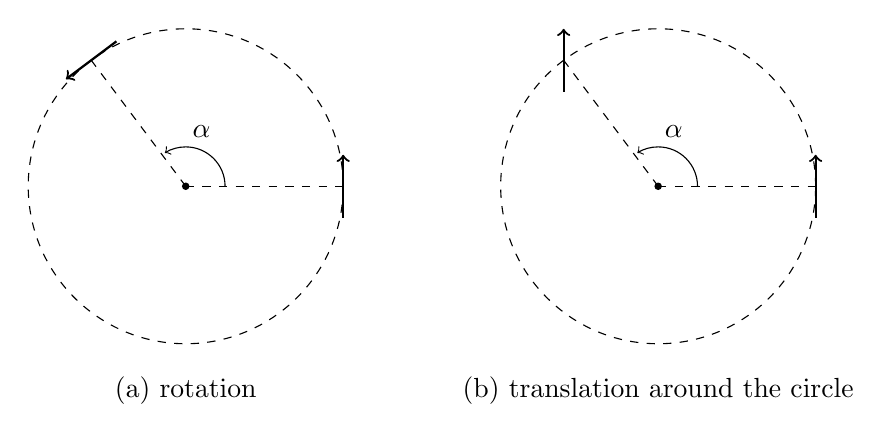
\begin{tikzpicture}
            \draw[fill=black] (0,0) circle (0.04);
            \draw[dashed] (0,0) circle (2);
            \draw[->,thick] (2,-0.4)--(2,0.4);
            \draw[dashed] (0,0)--(2,0);
            \draw[dashed] (0,0)--(-1.2,1.6);
            \draw[->,thick] (-0.88,1.84)--(-1.52,1.36);
            \draw[->] (0.5,0) arc (0:122:0.5);
            \node at (0.2,0.7) {\(\alpha\)};
            \node at (0,-2.6) {(a) rotation};

            \draw[fill=black] (6,0) circle (0.04);
            \draw[dashed] (6,0) circle (2);
            \draw[->,thick] (8,-0.4)--(8,0.4);
            \draw[dashed] (6,0)--(8,0);
            \draw[dashed] (6,0)--(4.8,1.6);
            \draw[->,thick] (4.8,1.2)--(4.8,2);
            \draw[->] (6.5,0) arc (0:122:0.5);
            \node at (6.2,0.7) {\(\alpha\)};
            \node at (6,-2.6) {(b) translation around the circle};
        \end{tikzpicture}
        \caption{The rotation operator \(U(\vb{\alpha})\) swings a system around the origin and also rotates its orientation in \(\RR^3\), while a circular translation merely moves the system around a circular path, without affecting its orientation. The difference is a rotation of the body around its own centre of mass, reorientating it without changing its location.}
        \label{Fig:rotation_circular_translation_difference}
    \end{figure}

    We define the \textit{spin} operator \(\vb{S}\) to be the difference
    \begin{equation}
        \vb{S}=\vb{J}-\vb{L}
    \end{equation}
    so that \(\vb{J}=\vb{L}+\vb{S}\). From \cref{Fig:rotation_circular_translation_difference} we see that difference between rotating an object around some fixed origin and a translating it's centre of mass along a circular path is a rotation around the object's centre of mass. generates a rotation of the body around its own centre of mass. We thus expect (and will confirm below) that \(\vb{S}\) generates rotations of a body around its own centre of mass, reorienting it in space. This is why \(\vb{S}\) is called the spin operator.

    In the case of a macroscopic body, made up of many constituent particles, it's reasonable to suppose that the spin operator just account for the difference between translating the body as a whole and translating each individual particle around their own arcs, with slightly different radii according to where in the body the particle is located. That is,
    \begin{equation}
        \vb{S}\stackrel{?}{=}\left(\sum_a\vb{X}_a\cross\vb{P}_a\right)-\vb{X}\cross\vb{P}=\sum_a\vb{x}_a\cross\vb{p}_a\,,
    \end{equation}
    where \(\vb{X}_a\) and \(\vb{P}_a\) are position and translation operators for each individual particle and \(\vb{x}_a\) and \(\vb{p}_a\) are their positions and momenta relative to the centre of mass\footnote{We'll understand how to properly describe the quantum mechanics of a system with many degrees of freedom (e.g. many particles) in \cref{Chap:Identical_Particles}.}. However, for an object consisting of many particles such a description is clearly going to be very cumbersome. More fundamentally, we do not know what the ``fundamental'' constituents of our object really are. (For example, if I sit on a merry-go-round, is the ``right'' quantum description of my motion given in terms of my cells, or my atoms, or protons and neutrons, or quarks and gluons, or bits of string, or ...?) It's thus crucial that we can consider objects as a whole in quantum mechanics, just as we can classically. For rotations, understanding \(\vb{S}\) will allow us to do this. In addition, as we'll see in \cref{Chap:Large_Rot}, one of the surprises of quantum mechanics is that even fundamental particles such as electrons and photons may have an ``intrinsic'' spin that (as far as we know) is not related to any composite structure.

    Fortunately, commutation relations involving the spin operator \(\vb{S}\) are easy to obtain from the ones we already have for \(\vb{J}\) and \(\vb{L}\). Firstly, the fundamental relations
    \begin{equation}
        [J_i,X_j]=\ii\hbar\sum_k \epsilon_{ijk}X_k\quad\text{and}\quad[J_i,P_j]=\ii\hbar\sum_k\epsilon_{ijk}P_k
    \end{equation}
    show that
    \begin{equation}
        [J_i,L_j]=\ii\hbar\sum_k \epsilon_{ijk}L_k\,,
    \end{equation}
    so that the angular momentum operator \(\vb{L}\) also transforms as a vector under rotations. Recalling from IB Quantum Mechanics that \([L_i,L_j]=\ii\hbar\sum_k\epsilon_{ijk}L_k\), we have
    \begin{align}
        [S_i,S_j]&=[J_i-L_i,J_j-L_j]=[J_i,J_j]-[J_i,L_j]-[L_i,J_j]+[L_i,L_j]\notag\\
        &=\ii\hbar\sum_{k}\epsilon_{ijk}(J_k-L_k)=\ii\hbar\sum_k\epsilon_{ijk}S_k\,.
    \end{align}
    It then immediately follows that \([\vb{S},\vb{S}^2]=0\). This algebra --- the same as that obeyed by the components of \(\vb{J}\) and \(\vb{L}\) --- confirms that the spin operator \(\vb{S}\) generate some form of rotation. On the other hand, since \([L_i,X_j]=\ii\hbar\sum_k\epsilon_{ijk}X_k\) and \([L_i,P_j]=\ii\hbar\sum_k\epsilon_{ijk}P_k\), we have
    \begin{align}
        [S_i,X_j]&=[J_i,X_j]-[L_i,X_j]=0\,,\\
        [S_i,P_j]&=[J_i,P_j]-[L_i,P_j]=0\,.
    \end{align}
    These commutation relations confirm that the spin operator has nothing to do with an object's location in or motion through space, but is purely to do with rotating its intrinsic orientation. Finally, since \(\vb{S}\) commutes with both \(\vb{X}\) and \(\vb{P}\), it also commutes with \(\vb{L}\):
    \begin{equation}
        [S_i,L_j]=0\quad\forall i,j\,.
    \end{equation}
    This allows us to factorize the operator \(U(\vb{\alpha})\) describing finite rotations as
    \begin{equation}
        U(\vb{\alpha})=\ee^{-\ii \vb{\alpha}\vdot\vb{J}/\hbar}=\ee^{-\ii \vb{\alpha}\vdot(\vb{L}+\vb{S})/\hbar}=\ee^{-\ii \vb{\alpha}\vdot\vb{L}/\hbar}\ee^{-\ii \vb{\alpha}\vdot\vb{S}/\hbar}=\ee^{-\ii \vb{\alpha}\vdot\vb{S}/\hbar}\ee^{-\ii \vb{\alpha}\vdot\vb{L}/\hbar}\,.
    \end{equation}
    As in \cref{Fig:rotation_circular_translation_difference}, these equations confirm that we can think of a quantum rotation as consisting of a translation of a body's centre of mass along an arc centred on the origin together with a simultaneous rotation of the body around its own centre of mass by the same amount. The order in which we perform these two operations makes no difference.

    \subsection{Time Translations}
    It's not only transformations of space that are represented on \(\hb\) by unitary operators. Consider translations in time. These again form an Abelian group, since sending \(t_0\) to \(t_0+t\) and then to \(t_0+t+t'\) gives the same end result as does \(t_0\mapsto t_0+t'\mapsto t_0+t'+t\). If we want the total probability of our particle being found somewhere in \(\RR^3\) at all times, then time translation must also be represented by a unitary operator \(U(t):\hb\to\hb\). Since we can translate through an arbitrarily small time, the time translation operator takes the form
    \begin{equation}
        U(t)=\exp\left(-\frac{\ii}{\hbar}Ht\right)\,,
    \end{equation}
    where \(H/\hbar\) must be Hermitian and is, by definition, the generator of time translations. This generator must have dimensions \(1/(\text{time})\), so the conventional factor of \(\hbar\) means that \(H\) itself has dimensions of energy. Of course, \(H\) will turn out to be the Hamiltonian, but for now I'd like you to think of it more abstractly just as the generator of time translations.

    The fact that \(U(t)\) represents the effect of a time translation on \(\hb\) means that if a particle is in some state \(\ket{\psi(0)}\) at time \(t_0=0\), translating forward to time \(t\) we will find it in the state
    \begin{equation}
        \ket{\psi(t)}=U(t)\ket{\psi(0)}=\ee^{-\ii Ht/\hbar}\ket{\psi(0)}\,.
    \end{equation}
    In particular, the difference between \(\ket{\psi(t)}\) and the state we find a short time later is
    \begin{equation}
        \ket{\psi(t+\delta t)}-\ket{\psi(t)}=-\frac{\ii}{\hbar}\delta tH\ket{\psi(t)}+U(\delta t^2)\,,
    \end{equation}
    or, taking the limit \(\delta t\to 0\),
    \begin{equation}
        \ii\hbar\pdv{}{t}\ket{\psi(t)}=H\ket{\psi(t)}\,.
    \end{equation}
    This, famously, is the time dependent Schr\"{o}dinger equation. It's just the infinitesimal version of the statement that all states in \(\hb\) evolve in time according to the action of a unitary operator \(U(t)\).

    \subsubsection{The Heisenberg Picture}
    In IB Quantum Mechanics, we were used to the idea that states evolve in time according to the time dependent Schr\"{o}dinger equation. However, just as we did for spatial transformations, we can instead work in a picture where the states are time independent and instead the operators evolve in time. To see how this works, suppose \(O_S\) is some operator that contains no explicit time dependence. Then the amplitude for the state \(O_S\ket{\psi(t)}\) to agree at time \(t\) with the state \(\ket{\chi(t)}\) is
    \begin{equation}\label{Heisenberg_picture}
        \mel{\chi(t)}{O_S}{\psi(t)}=\mel{\chi(0)}{U^{-1}(t)O_S U(t)}{\psi(0)}\,.
    \end{equation}
    The right hand side here only makes explicit reference to the initial values of the states \(\ket{\psi}\) and \(\ket{\chi}\). Since it holds true for any pair of states, just as above we can obtain the same results by always working with the initial states and instead evolving the operators as
    \begin{equation}
        O_H(t)=U^{-1}(t)O_S U(t)\,.
    \end{equation}
    The version of quantum mechanics where we use the time dependent Schr\"{o}dinger equation to evolve the states in time, leaving operators unaltered, is known as the Schr\"{o}dinger picture, whereas the version where the states are fixed at their initial values and instead the operators evolve in time is called the Heisenberg picture.

    In fact, all this has a precise analogue in classical mechanics. Classically, there are also two ways of thinking about time evolution. On the one hand, we can think of a particle moving in some way through phase space \(M\). If we know it's location \((\vb{x}(t),\vb{p}(t))\in M\) for every time \(t\) we can compute any quantity we wish, represented by some function \(f:M\to\RR\), by evaluating \(f\) at the location of our particle, obtaining the value \(f(\vb{x}(t),\vb{p}(t))\). (This is the perspective we took in the Introduction.) However, Newton's Laws are deterministic, so, given a force, the entire trajectory is determined by the initial conditions \((\vb{x}_0,\vb{p}_0)\). This suggests a perspective in which the ``state'' of our particle is simply a choice of initial conditions. These initial conditions do not themselves evolve, rather, it is the quantities we measure that vary in time. Thus, instead of thinking of a physical quantity \(f\) as a map from phase space, we treat it just as a map from time, so \(f:[t_0,\infty)\to\RR\). You'll examine these classical pictures further if you're taking the Classical Dynamics course, in the context of Hamiltonian mechanics. (It's really for this reformulation of classical mechanics, not the particular \(H\), that Hamilton is famous.)

    Differentiating (\ref{Heisenberg_picture}) with respect to \(t\) by product rule shows that
    \begin{align}
        \dv{}{t} O_H(t)&=\dv{}{t}(U^{-1}(t)O_S U(t))=\frac{\ii}{\hbar}(U^{-1}(t)HO_SU(t)-U^{-1}O_SHU(t))\notag\\
        &=\frac{\ii}{\hbar}[H,O_H(t)]\,,\label{Heisenberg_equation_of_motion}
    \end{align}
    where in the last step we used the fact that \([U(t),H]=0\), since \(U(t)\) depends only on \(H\). This is the \textit{Heisenberg equation of motion}. It's completely equivalent to the Schr\"{o}dinger equation, and is also just a (very important) special case of our general argument of how operators transform under the action of unitary groups of transformations. More generally, if the original operator \(O_S\) had some explicit time dependence of its own --- independent of any particular particle's motion --- then we would obtain a further term in this equation, modifying it to
    \begin{equation}
        \dv{}{t}O_H(t)=U^{-1}(t)\pdv{O_S}{t}U(t)+\frac{\ii}{\hbar}[H,O_H(t)]\,.
    \end{equation}
    For example, we may wish to understand the behaviour of a charged particle in the presence of an applied electric field. If the electric field is itself changing in time, then the potential in which the particle moves will be time-dependent even in the Schr\"{o}dinger picture.

    \subsection{Dynamics}
    So far, we've simply defined some unitary operators \(U(\vb{a})\), \(U(\vb{\alpha})\) and \(U(t)\) that are responsible for translating, rotating or evolving our system through space and time. The commutation relations of the generators \(\vb{P}\) and \(\vb{J}\), and their commutation relations with \(\vb{X}\) were determined purely by the properties of the corresponding group of transformations of \(\RR^3\). However, while we've seen that commutators such as \([H,\vb{X}]\), \([H,\vb{P}]\) and \([H,\vb{J}]\) are important in the Heisenberg picture, telling us how these operators change in time, we haven't yet given any way to actually calculate what such commutators should be. Similarly, although we've said that in the Schr\"{o}dinger picture, states evolve in time according to \(\ket{\psi(t)}=U(t)\ket{\psi(0)}\), we haven't given any way to work out what the action of the generator \(H\) on a state should actually be.

    To do so, we must specify the dynamics: we must provide a relation \(H=H(\vb{X},\vb{P})\) giving \(H\) in terms of the other operators whose commutators we already understand. The simplest (non-trivial) example of such relation is\footnote{Note that this is the first time we've pinned ourselves down to a non-relativistic theory. Up to this point, everything we've said holds good in relativistic quantum mechanics and, suitably interpreted, also in quantum field theory. In the lectures we studied translations and rotations, and you can extend this to also consider Galilean boosts and can show that the non-relativistic Hamiltonian is compatible with the Galilean algebra. If one instead wishes to study a relativistic version of quantum theory, one starts by finding unitary operators representing the action of the Poincar\'{e} group \(\RR^{3,1}\rtimes \SO(3,1)\) of special relativity. The relation (\ref{kinetic_Hamiltonian}) between \(H\) and \(\vb{P}\) does not respect the commutation relations appropriate for Poincar\'{e} symmetry, but of course the dynamical relation \(H^2=c^2\vb{P}^2+m^2c^4\) does. The difficulty with relativistic quantum mechanics lies not with symmetries, but with interactions. The proper treatment of these requires Quantum Field Theory, a far deeper subject.}
    \begin{equation}\label{kinetic_Hamiltonian}
        H=\frac{1}{2m}\vb{P}^2
    \end{equation}
    where \(m\) is a constant with dimensions of mass. Equation (\ref{kinetic_Hamiltonian}) relates how a state evolves in time (via \(H\)) to how its location is translated through space (via \(\vb{P}\)); in other words, it's telling us something about how particles move! In particular, with this form of Hamiltonian the difference between the expected location of a state \(\ket{\psi}\) at an initial time and a short time \(\delta t\) later is
    \begin{align}
        \expval{U^{-1}(\delta t)\vb{X}U(\delta t)}{\psi}-\expval{\vb{X}}{\psi}&=\frac{\ii}{\hbar}\delta t\expval{[H,\vb{X}]}{\psi}+O(\delta t^2)\notag\\
        &=\frac{\delta t}{m}\expval{\vb{P}}{\psi}+O(\delta t^2)\,.
    \end{align}
    In the limit \(\delta t\to 0\), we see that the expected velocity of the particle is \(\expval{\vb{P}}{\psi}/m\). Equivalently, since this is true for all \(\ket{\psi}\in\hb\), we can write
    \begin{equation}
        \dv{}{t}\vb{X}(t)=\frac{\vb{P}(t)}{m}
    \end{equation}
    in the Heisenberg picture. Furthermore, since \([H,\vb{P}]=0\) for this Hamiltonian, \(P(t)=P(0)\) and all states travel in uniform motion.

    In the real world, we observe that particles do not always travel with constant velocities: they may slow down, speed up, or change direction as they encounter various obstacles. These obstacles are typically located at various different points in space. To allow for this, we generalise our dynamical relation (\ref{kinetic_Hamiltonian}) to
    \begin{equation}\label{kinetic_potential_Hamiltonian}
        H=\frac{1}{2m}\vb{P}^2+V(\vb{X})\,.
    \end{equation}
    The first term on the right is the kinetic term and is the contribution to the Hamiltonian due to the state is traveling through space. The second, potential term is the contribution due to the state's location. This familiar form is still a very special case of the general statement \(H=H(\vb{X},\vb{P})\) and later in the course we'll meet examples of Hamiltonians that don't fit this form.

    Repeating the calculation we still find that \(\mathrm{d} \vb{X}(t)/\mathrm{d} t=\vb{P}(t)/m\), but now \([H,\vb{P}]\ne 0\) so the rate of motion through space will not always be the same. Rather, using (\ref{Heisenberg_equation_of_motion}), the Heisenberg picture operators obey
    \begin{equation}\label{Heisenberg_momentum}
        \dv{}{t}\vb{P}(t)=\frac{\ii}{\hbar}[H,\vb{P}(t)]=-\grad V(t)\,,
    \end{equation}
    where \(\grad V(t)=U^{-1}(t)(\partial V/\partial \vb{X})U(t)=-\grad V(\vb{X}(t))\). Thus the motion slows down or speeds up according to the gradient of \(V(\vb{X})\).
    
    Most of our common intuition about momentum comes from equation (\ref{Heisenberg_momentum}). We ``feel'' that a tennis ball traveling with a certain speed has less momentum than a cannonball traveling with the same speed, and less than the same tennis ball traveling faster, because we've known from an early age that it will cause us less damage to stand in the way of the first tennis ball than either of the other two. This is really a statement about what our unfortunate bodies will have to do in order to bring these projectiles to rest (or how much effort we will have to exert to launch them in the first place). In other words, our intuitive notion of momentum is built on a feeling for the energy our body will gain as we slow the projectile down during the impact. This energy then excites the atoms that ultimately make up our nerves, muscles and bones, becoming dissipated through our bodies. Ultimately, it is the dynamical relation between the Hamiltonian and other operators that justifies us identifying the operator \(\vb{P}/\hbar\) --- by definition, the generator of translations --- with our pre-existing notion of momentum (in units of \(\hbar\)). Only after we specify our dynamics do commutation relations such as \([X_i,P_j]=\ii\hbar\delta_{ij}\) tell us, via Born's \(2^\text{nd}\) postulate of Quantum Mechanics, that a particle cannot simultaneously be in a state of well-defined position and of well-defined momentum.

    We'll often find it useful to write the kinetic term in a slightly different form. Keeping careful track of the operator ordering, you'll show in the problem set that
    \begin{equation}
        \vb{L}^2=(\vb{X}\cross\vb{P})\vdot(\vb{X}\cross\vb{P})=\vb{X}^2(\vb{P}^2-P_r^2)\,,
    \end{equation}
    where for \(\vu{X}=\vb{X}/\norm{\vb{X}}\),
    \begin{equation}
        P_r=\frac{1}{2}\left(\vu{X}\vdot\vb{P}+\vb{P}\vdot\vu{X}\right)
    \end{equation}
    is the radial angular momentum operator. Consequently, we can write the Hamiltonian (\ref{kinetic_potential_Hamiltonian}) in terms of the generator of circular translations and the radial momentum operator \(P_r\) as
    \begin{equation}
        H=\frac{P_r^2}{2m}+\frac{\vb{L}^2}{2m\vb{X}^2}+V(\vb{X})\,,
    \end{equation}
    where we note that \([\vb{L},\vb{X}^2]=0\), so the order of the second term is irrelevant provided we keep \(\vb{X}^2\) together as a composite operator. (In particular, in the position representation, \(\vb{X}^2\) acts as multiplication by \(\vb{x}^2=r^2\), which is certainly unaffected by translation in a circle.) Most of our intuitive feeling about angular momentum --- like our happy childhood hours spent on merry-go-rounds --- is encapsulated in this relation between the Hamiltonian and \(\vb{L}^2\). Again, it's the form of the Hamiltonian which is the basis of our identification of the generator \(\vb{L}/\hbar\) of circular transformations with angular momentum (in units of \(\hbar\)). 

    \subsubsection{Symmetries and Conservation Laws}
    One of the immediate uses of the Heisenberg picture is to deduce a relation between symmetries and conserved quantities\footnote{In Classical Dynamics course, you will see a corresponding relation in Hamilton's approach to classical physics}. If it happens that an operator \(Q\) commutes with the Hamiltonian, then it also commutes with \(\ee^{-\ii Ht/\hbar}\), so the Heisenberg picture operator
    \begin{equation}
        Q(t)=U^{-1}(t)QU(t)=U^{-1}U(t)Q=Q\,,
    \end{equation}
    coinciding with the Schr\"{o}dinger operator at all \(t\). Infinitesimally, provided \(Q\) has no explicit time dependence, this is
    \begin{equation}\label{conversed_operator}
        \dv{}{t}Q(t)=\frac{\ii}{\hbar}[H,Q(t)]=\frac{\ii}{\hbar}U^{-1}(t)[H,Q]U(t)=0\,.
    \end{equation}
    Operators that are time independent even in the Heisenberg picture are said to be conserved. We've shown that conserved operators are just that commute with the Hamiltonian.

    Suppose we prepare a particle to be in an eigenstate of some conversed operator at time \(t=0\), so \(Q\ket{\psi(0)}=q\ket{\psi(0)}\). Then at any later time we have
    \begin{equation}
        Q\ket{\psi(t)}=QU(t)\ket{\psi(0)}=U(t)Q\ket{\psi(0)}=qU(t)\ket{\psi(0)}=q\ket{\psi(t)}
    \end{equation}
    so our particle remains in an eigenstate of \(Q\) at all subsequent times (provided the state evolves according to the time-dependent Schr\"{o}dinger equation). For this reason, it's usually sensible to expand our states in a basis of eigenstates of a maximal set of conserved operators, rather than a maximal commuting set of any old operators. We label the states in this basis by their corresponding eigenvalues, because the same labelling will remain valid at subsequent times. For example, provided \(H\) has no explicit time dependence\footnote{Even if the Hamiltonian does contain explicit time dependence, for example because it describes the dynamics of a charged particle in a varying electric field, \([H(t),H(t)]=0\) trivially. However, \([H(t'),H(t)]\) may not vanish as the form of the Hamiltonian itself changes.} \([H,H]=0\) trivially, so the Hamiltonian itself is always conserved, and it is often useful to work in a basis of energy eigenstates.

    By far the most important source of conserved quantities is symmetries of the Hamiltonian. These are transformations that leave the Hamiltonian invariant. We've seen that a generic unitary operator \(U(\theta)=\ee^{\ii \theta T}\) representing some transformation of space on \(H\) acts on operators as in equation (\ref{transformed_operator}). In particular, its action on the Hamiltonian is
    \begin{equation}
        H\longmapsto U^{-1}(\theta)HU(\theta)\,.
    \end{equation}
    If the Hamiltonian is invariant under this transformation --- i.e. if the transformation is a symmetry --- then
    \begin{equation}
        U^{-1}(\theta)HU(\theta)=H\,,
    \end{equation}
    or equivalently
    \begin{equation}
        [T,H]=0
    \end{equation}
    for an infinitesimal symmetry transformation, where \(T\) is the Hermitian generator. This is exactly the same condition (\ref{conversed_operator}) we had for the generator \(T\) to be conserved, so symmetries of the Hamiltonian correspond to conserved quantities\footnote{In the Classical Dynamics or Integrable Systems courses, you'll meet the corresponding statement in classical mechanics in called N\"{o}ther's theorem.}.
    For example, if the Hamiltonian is translationally invariant then \([\vb{P},H]=0\), so for such Hamiltonians, momentum will be conserved. Note that it's not necessary for the Hamiltonian to be independent of each particle's position \(\vb{x}_a\) if \(H\) is to be translationally invariant, as long as any potential term \(V(\vb{x}_a,\vb{x}_b)\) depends only on the relative positions. Similarly, if the Hamiltonian is rotationally invariant then \([\vb{J},H]=0\) so angular momentum will be conserved. In this case, \(J_z, J^2\) and \(H\) form a set of mutually commuting operators, so we can expand a general state in a basis \(\{\ket{n,\ell,m,\dots}\}\) where the labels \((n,\ell,m)\) refer to the eigenvalues of \(H\), \(J^2\) and \(J_z\). We've left open the possibility that our states have further conserved properties, indexed by further labels. These will often contain information about the ``internal'' state of our system.

    \subsection{Parity}\label{Chap:Parity}
    Not all transformations are continuous. In physics, the most prominent example of a discrete transformation is the \textit{parity transformation} \(\mathcal{P}\), acting on \(\RR^3\) as \(\mathcal{P}:\vb{x}\mapsto-\vb{x}\). Since \(\det(\mathcal{P})=-1\), this is different from a rotation, so may have consequences that cannot be deduced by considering only rotations.

    On Hilbert space, parity transformations will still be represented by a unitary operator, but this operator will no longer involve a parameter that may be taken infinitesimally small. Consequently there's no generator associated with parity transformations. Calling the unitary parity operator \(\Pi\), we have
    \[\Pi^{-1}\vb{X}\Pi=\mathcal{P}\vb{X}=-\vb{X}\]
    as its defining property. Multiplying through on the right by \(\Pi\), we can also write this as
    \begin{equation}
        \{\Pi,\vb{X}\}\coloneqq\Pi\vb{X}+\vb{X}\Pi=0\,,
    \end{equation}
    where the bracket \(\{A,B\}\) is the \textit{anticommutator} of \(A\) and \(B\). Translating through \(\vb{a}\) then applying the parity operator \(\mathcal{P}:\RR^3\to\RR^3\) is the same as first applying \(\mathcal{P}\), then translating through \(-\vb{a}\), so
    \begin{equation}
        \Pi^{-1}U(\vb{a})\Pi=U(-\vb{a})\,,
    \end{equation}
    so that the momentum operator also anticommutes with the parity operator: \(\Pi^{-1}\vb{P}\Pi=-\vb{P}\). More generally, if \(\vb{V}\) is any vector that transforms as a vector under rotations, we say \(\vb{V}\) is a \textit{vector operator} if also
    \begin{equation}\label{parity_inversion_vector}
        \Pi^{-1}\vb{V}\Pi=-\vb{V}\,,
    \end{equation}
    so that \(\{\Pi,\vb{V}\}=0\). If instead
    \begin{equation}
        \Pi^{-1}\vb{V}\Pi=+\vb{V}\,,
    \end{equation}
    so equivalently \([\Pi,\vb{V}]=0\), then \(\vb{V}\) is a \textit{pseudovector operator} (provided it transforms appropriately under rotations). The most prominent example of a pseudovector operator is the rotation generator \(\vb{J}\): since the parity transformation \(\mathcal{P}\) acts on \(\RR^3\) as \(-\Id_{3\times 3}\), rotations obey \(\mathsf{R}(\vb{\alpha})\mathcal{P}=\mathcal{P}\mathsf{R}(\vb{\alpha})\), or \(\mathcal{P}^{-1}\mathsf{R}(\vb{\alpha})\mathcal{P}=\mathsf{R}(\vb{\alpha})\). This gives
    \begin{equation}
        \Pi^{-1}U(\vb{\alpha})\Pi=U(\vb{\alpha})
    \end{equation}
    for the parity and rotation operators in the Hilbert space, or \(\Pi^{-1}\vb{J}\Pi=\vb{J}\) for the rotation generator. Likewise, the orbital angular momentum operator obeys
    \begin{equation}
        \Pi^{-1}\vb{L}\Pi=\Pi^{-1}(\vb{X}\cross\vb{P})\Pi^{-1}=(\Pi^{-1}\vb{X}\Pi)\cross(\Pi^{-1}\vb{P}\Pi)=(-\vb{X})\cross(-\vb{P})=\vb{L}\,,
    \end{equation}
    so it is a pseudovector as in classical mechanics. It follows that the spin operator \(\vb{S}=\vb{J}-\vb{L}\) is also a pseudovector.

    Similarly, operators \(S\) that are invariant under rotations are scalar operators if in addition \(\Pi S\Pi=S\) so that they are unchanged under parity, and are pseudoscalar operators if instead \(\Pi S\Pi= S\). (Notice that the signs for scalars and pseudoscalars are the opposite way round to those for vectors and pseudovectors.) As usual, the parity of a system will be conserved if \([H,\Pi]=0\). As a simple example, if our system is governed by the dynamical relation \(H=\vb{P}^2/2m +V(\vb{X})\) where the potential is an even function, then
    \begin{align}
        \Pi^{-1}H\Pi&=\frac{1}{2m}(\Pi^{-1}\vb{P}\Pi)\vdot(\Pi^{-1}\vb{P}\Pi^{-1})+\Pi^{-1}V(\vb{X})\Pi\\
        &=\frac{\vb{P}^2}{2m}+V(\Pi^{-1}\vb{X}\Pi)\\
        &=\frac{\vb{P}^2}{2m}+V(\vb{X})=H\,,
    \end{align}
    so parity is conserved for such Hamiltonians.

    Parity transformations form the group \(G=\ZZ_2\), since carrying out a non-trivial parity transformation twice just brings us back to where we were. Thus \(P_2=1_{\RR^3}\) and applying our homomorphism shows that
    \begin{equation}
        \Pi^2=1_{\hb}
    \end{equation}
    for the parity operator on Hilbert space, too. Now suppose that \(\ket{\psi}\) is an eigenstate of \(\Pi\) with eigenvalue \(\eta\). Then\footnote{This argument is adequate for our course, and leads to a correct conclusion, but it hides a number of subtleties. See e.g. Weinberg The Quantum Theory of Fields, vol. 1, section 4.7 for a fuller discussion.}
    \begin{equation}
        \ket{\psi}=\Pi^2\ket{\psi}=\eta\Pi\ket{\psi}=\eta^2\ket{\psi}\,,
    \end{equation}
    so the spectrum of \(\Pi\) is just \(\{+1,-1\}\).

    If \(\ket{\vb{v}}\) is an eigenstate of a vector operator \(\vb{V}\), with \(\vb{V}\ket{\vb{v}}=\vb{v}\ket{\vb{v}}\), then from \ref{parity_inversion_vector}, the parity reversed state \(\ket{\vb{v}'}=\Pi\ket{\vb{v}}\) obeys
    \begin{equation}
        \vb{V}\ket{\vb{v}'}=\vb{V}\Pi\ket{\vb{v}}=-\Pi\vb{V}\ket{\vb{v}}=-\vb{v}\Pi\ket{\vb{v}}=-\vb{v}\ket{\vb{v}'}
    \end{equation}
    so is also an eigenstate of \(\vb{V}\), but with opposite sign eigenvalue. In particular, \(\Pi\ket{\vb{x}}\) is an eigenstate of the position operator with eigenvalue \(-\vb{x}\), so
    \begin{equation}
        \Pi\ket{\vb{x}}=c\ket{-\vb{x}}
    \end{equation}
    for some constant \(c\in\CC\). This is not an eigenvalue equation, because the right hand side involves \(\ket{-\vb{x}}\) rather than \(\ket{\vb{x}}\). However, we can immediately identify \(c\) with \(\eta\) because applying \(\Pi\) a second time gives\footnote{Note that it is important here that \(\Pi\ket{\vb{x}}=c\ket{-\vb{x}}\) for all values of \(\vb{x}\).}
    \begin{equation}
        \ket{\vb{x}}=\Pi^2\ket{\vb{x}}=c^2\ket{\vb{x}}\,,
    \end{equation}
    so again \(c^2=1\) and \(c=\pm 1\). More generally, given any state \(\ket{\psi}\), the wavefunction of the parity transformed state \(\Pi\ket{\psi}\) is
    \begin{equation}
        \mel{\vb{x}}{\Pi}{\psi}=\eta^{-1}\braket{-\vb{x}}{\psi}=\eta\psi(-\vb{x})\,,
    \end{equation}
    so, up to a sign, the wavefunction of the new state takes the same value at \(\vb{x}\) as the original one did at \(-\vb{x}\).

    For example, suppose that for some particle, \(\ket{\vb{x}}\) obey \(\Pi\ket{\vb{x}}=\ket{-\vb{x}}\), with \(\eta=+1\). Recalling from IB Quantum Mechanics that the spherical harmonics \(Y_\ell^m(\vb{x})\) obey \(Y_\ell^m(-\vb{x})=(-1)^\ell Y_\ell^m(\vb{x})\), we see that if this particle is in the state \(\ket{n,\ell,m}\) whose wavefunction \(\braket{\vb{x}}{n,\ell,m}=R_n(\abs{\vb{x}})Y_\ell^m(\vb{x})\) (where the radial part \(R_n(r)\) of the wavefunction determines the energy level \(n\)), applying the parity operator gives
    \begin{equation}\label{spherical_harmonics_parity}
        \mel{\vb{x}}{\Pi}{n,\ell,m}=\braket{-\vb{x}}{n,\ell,m}=(-1)^\ell\braket{\vb{x}}{n,\ell,m}
    \end{equation}
    and consequently \(\Pi\ket{n,\ell,m}=(-1)^\ell\ket{n,\ell,m}\).

    Parity transformations act in a more complicated way on macroscopic objects, or systems with some internal structure. This is clear classically: the parity transformation of a book initially located at \(\vb{x}\) is not simply a book located at \(-\vb{x}\), but rather a mirror image (simultaneously left-right, up-down and front-back) of the book. As with the distinction between \(\vb{J}\) and \(\vb{L}\), for a macroscopic body we might hope to account for this by defining a separate parity operator for each constituent particle. However, it turns out that subatomic particles such as the photon or pion have their own ``intrinsic'' parities. Thus, whether a given \(\Pi\)-eigenstate has \(\eta=+1\) or \(\eta=-1\) depends not only on details of the spatial wavefunction, but also on the species of particle the state describes.
    
    We'll explore intrinsic parity further in \cref{intrinsic_parity}, but as an example of its use, consider transitions between different energy levels of an atom. These are usually mediated by electromagnetic interactions: during such a transition, the atom's electrons either emit or absorb a photon whose energy \(\hbar\omega\) is equal to the difference in energy \(E\) between the two levels involved in the transition. As we'll study in more detail later, when the corresponding wavelength is much larger than the typical size of the atom, the transition rate \(\Gamma(i\to f)\) is given by
    \begin{equation}
        \Gamma(i\to f)=\frac{4(\Delta E)^3}{c^3\hbar^4}\abs{\mel{f}{\vb{D}}{i}}^2\,,
    \end{equation}
    where \(\ket{i}\) and \(\ket{f}\) are the initial and final states of the atom, and \(\vb{D}=\sum e_a\vb{X}_a\) is the operator corresponding to the atom's electric dipole moment. (The sum runs over all the electrons in the atom.) Reversing the parity of space affects all the electrons equally, so the parity operator obeys \(\Pi^{-1}\vb{X}_a\Pi=-\vb{X}_a\) for each \(\vb{X}_a\). Thus \(\Pi\vb{D}\Pi=-\vb{D}\).

    Now suppose that the initial and final states of the atom are eigenstates of \(\Pi\), with eigenvalues \(\eta_i\) and \(\eta_f\), respectively. Then\footnote{Note that since the parity operator \(\Pi\) is unitary, its quantum numbers \(\eta\) behave multiplicatively, whilst those of a Hermitian generator of a continuous symmetry (such as \(P\)) behave additively.}
    \begin{equation}
        \eta_i\eta_f\mel{f}{\vb{D}}{i}=\mel{f}{\Pi^{-1}\vb{D}\Pi}{i}=-\mel{f}{\vb{D}}{i}
    \end{equation}
    so the amplitude for the transition will vanish unless the initial and final atomic states have opposite parity, \(\eta_i\eta_f=1\). In the most common case, just a single electron is involved in the transition and in this case equation (\ref{spherical_harmonics_parity}) shows that \(\eta_i\eta_f=(-1)^{l_i+l_f}\), where \(\ell_i,\ell_f\) are the total orbital angular momentum quantum numbers of the initial and final states of this electron. Thus, in any radiative atomic transition involving just a single electron, the orbital angular momentum quantum number \(\ell\) must change by an odd number. If our initial and final states kept track of the photon as well as the atom, we'd be able to say overall parity is conserved in such transitions if we assign an intrinsic parity \(-1\) to the photon that is emitted or absorbed in the transition. (The intrinsic parity of the photon is related to the fact that the electromagnetic vector potential \(\vb{A}\), whose quantum version provides the description of the photon, indeed transforms as a vector, not a pseudovector.) In fact, \([H,\Pi]=0\) holds in general for particles travelling in the presence of any type of electromagnetic interaction.

    Having \([H,\Pi]\) be zero means that if at time \(t=0\) you set up a system to be a mirror image of another system, then their subsequent evolution will be identical in the sense that if you observe them at a later time, they will still be mirror images of one another. Hence, when \([H,\Pi]=0\) it is impossible to tell whether a system is being observed directly or through a mirror. One of the major surprises of twentieth-century physics was an experiment by Wu \textit{et al.} in 1957, which showed that in fact the Hamiltonian of our Universe has \([H,\Pi]\ne 0\) --- you can see things in a mirror that are impossible in our World!

    \newpage
    \section{Angular Momentum}
    In the previous chapter we obtained the fundamental commutation relations among the position, momentum and angular momentum operators, together with an understanding of how a dynamical relation \(H=H(\vb{X},\vb{P})\) allow us to understand how such quantities evolve in time. However, with the exception of the parity operator, we have not yet said anything about the spectrum --- the set of possible eigenvalues --- of these operators, nor have we been specific about the precise Hilbert space on which they act. Answering such questions is an important part of the subject of representation theory in mathematics; the study of how group actions can be realised on a given vector space. In physics, understanding this will provide essential information about the nature of our quantum system.

    To a large extent, both questions are determined by the operator algebra itself. For example, taking the trace of the commutation relations \([X_i,P_j]=\ii\hbar \delta_{ij}I_{\hb}\) in any finite dimensional Hilbert space \(\hb\) gives
    \begin{equation}
        \dim(\hb)\delta_{ij}=-\frac{\ii}{\hbar}\tr_{\hb}(X_i P_j-P_j X_i)=0
    \end{equation}
    for all \(i,j\) by the cyclic property of the trace. So there is no realisation of the position and translation operators on any non-trivial finite dimensional Hilbert space (and if \(\dim(\hb)=0\) then \(\vb{X}\) and \(\vb{P}\) necessarily act trivially). The above argument fails in an infinite dimensional Hilbert space, where neither \(\tr_{\hb}(I_\hb)\) nor \(\tr_\hb (X_i P_j)\) is defined. Thus, if we wish to discuss the position and momentum of a quantum system, we are necessarily in the world of function space.\footnote{Even here we should really be more careful. As mentioned in a previous footnote, \(\vb{X}\) and \(\vb{P}\) are not defined as linear operators on the whole of a Hilbert space such as \(L^2(\RR^3,\d[3]{x})\), because a state that is initially square-integrable may not remain so after the application of the unbounded operator \(\vb{X}\) or \(\vb{P}\).}

    On the other hand, taking the trace of the commutation relations
    \begin{equation}
        [J_i,J_j]=\ii\hbar\sum_k\epsilon_{ijk}J_k
    \end{equation}
    for the rotation generators just gives
    \begin{equation}
        \ii\hbar\epsilon_{ijk}\tr_{\hb}(J_k)=\tr_{\hb}(J_iJ_j-J_jJ_i)=0\,,
    \end{equation}
    so it is possible to represent each component of \(\vb{J}\) on a finite dimensional Hilbert space in terms of a traceless matrix\footnote{This traceless condition in \(\hb\) is closely related to but distinct from the fact that the generators of \(\SO(3)\) can also be represented by antisymmetric (hence traceless) matrices acting on \(\RR^3\).}. This is often a useful thing to do, particularly when discussing the internal structure of a system.

    In this chapter, we'll consider finite dimensional Hilbert spaces \(\hb_j\) whose elements transform among themselves under rotations. In mathematics, the \(\hb_j\) are known as \textit{irreducible representations} of the rotation group, whilst in physics they're called multiplets of definite total angular momentum. This chapter will also substantiate the link between the rotation generators \(\vb{J}\) and the physics of angular momentum, by examining a simple Hamiltonian for rotating diatomic molecule. We'll also flesh out the details of exactly how the orientation of a system is encoded in the amplitudes for it to be found in different eigenstates of appropriate angular momentum operators.

    \subsection{Angular Momentum Eigenstates}
    Let's begin by seeing how the algebra \([J_i,J_j]=\ii\hbar\sum_k\epsilon_{ijk}J_k\) determines the spectrum of the angular momentum operators. Since no two components of \(\vb{J}\) commute, we cannot find a complete set of simultaneous eigenstates of two components of \(\vb{J}\). However, since \([\vb{J},\vb{J}^2]=0\) we can find a complete set of simultaneous eigenstates of any one component of \(\vb{J}\) and \(\vb{J}^2\). Without loss of generality, we orient our coordinate system so that the chosen component of \(\vb{J}\) is \(J_z\). We let \(\ket{\beta,m}\) denote a simultaneous eigenstate of \(J_z\) and \(\vb{J}^2\), where
    \begin{equation}
        \vb{J}^2\ket{\beta,m}=\beta\hbar^2\ket{\beta,m}\qquad J_z\ket{\beta,m}=m\hbar\ket{\beta,m}
    \end{equation}
    and the factors of \(\hbar\) are for later convenience. We also choose all the states \(\ket{\beta,m}\) to be properly normalised. Since they are eigenstates of Hermitian operators, they must then be orthonormal
    \begin{equation}
        \braket{\beta',m'}{\beta,m}=\delta_{\beta\beta'}\delta_{mm'}\,.
    \end{equation}
    Finally, since we are looking for the simplest possible way to realize our commutation relations, we'll assume that the states \(\{\ket{\beta,m}\}\) are non-degenerate; that is, we want a Hilbert space where \(\ket{\beta,m}\) is the unique eigenstate of \(\vb{J}^2\) and \(J_z\) with the given eigenvalues. We'll comment more on this assumption in the next chapter.

    We now define
    \begin{equation}
        J_{\pm}=J_{x}\pm \ii J_y\,,
    \end{equation}
    which obey \(J_\pm^\dagger=J_\mp\) and so they are each other's adjoint. As they are built from linear combinations of the components of \(\vb{J}\), clearly \(J_\pm\) each commute with \(\vb{J}^2\), while their commutation relations with \(J_z\) are
    \begin{equation}
        [J_z,J_\pm]=[J_z,J_x]\pm \ii[J_z,J_y]=\ii\hbar(J_y\mp iJ_x)=\pm\hbar J_\pm\,.
    \end{equation}
    We learn that
    \begin{equation}
        \vb{J}^2(J_\pm\ket{\beta,m})=J_\pm\vb{J}^2\ket{\beta,m}=\hbar^2\beta J_\pm \ket{\beta,m}
    \end{equation}
    and
    \begin{equation}
        J_z(J_\pm\ket{\beta,m})=([J_z,J_\pm]+J_\pm J_z)\ket{\beta,m}=(m\pm 1)\hbar(J_\pm\ket{\beta,m})\,.
    \end{equation}
    These show that the new states \(J_\pm\ket{\beta,m}\), if not zero, are still eigenstates of both \(\vb{J}^2\) and \(J_z\), with the same eigenvalues \(\beta\hbar^2\) for \(\vb{J}^2\). However, their \(J_z\) eigenvalue is shifted up or down (respectively for \(J_+\ket{\beta,m}\) and \(J_-\ket{\beta,m}\)) by one unit of \(\hbar\). We see that the role of \(J_\pm\) in angular momentum is similar to the role of \(A\) and \(A^\dagger\) for energy of the harmonic oscillator. Again, \(J_+\) and \(J_-\) are often called the \textit{raising} and \textit{lowering operators}. Their role is to rotate our system, aligning more or less of its total angular momentum along the \(z\)-axis without
    changing the total angular momentum available.

    Just as for the harmonic oscillator, examining the algebra of our raising and lowering operators has told us the separation between angular momentum eigenstates, given a starting point \(\ket{\beta,m}\). To fix our initial states, we must examine the norm. By assumption, \(\ket{\beta,m}\) itself is correctly normalized and we compute
    \begin{align}
        \norm{J_+\ket{\beta,m}}^2&=\expval{J_-J_+}{\beta,m}=\expval{(J_x-\ii J_y)(J_x+\ii J_y)}{\beta,m}\notag\\
        &=\expval{\vb{J}^2-J_z^2-\hbar J_z}{\beta,m}=\hbar^2(\beta-m(m+1))\,.
    \end{align}
    But since this is a norm, whatever state \(\ket{\beta,m}\) we started we must have
    \begin{equation}
        \norm{J_+\ket{\beta,m}}^2=\beta-m(m+1)\ge 0\,,
    \end{equation}
    with equality iff \(J_+\ket{\beta,m}=0\) is the trivial state. This shows that it cannot be possible to keep applying \(J_+\), repeatedly raising \(J_z\) eigenvalue \(m\) while leaving \(\beta\). There must be some maximum value of \(m\) --- let's call it \(j\) --- for which \(J_+\ket{\beta,j}=0\). This can only be the case if \(\beta\) obeys
    \begin{equation}
        \beta=j(j+1)
    \end{equation}
    and so is fixed in terms of the maximum allowed value of \(m\).

    Similarly for a generic \(m\) value we find
    \begin{equation}
        \norm{J_-\ket{\beta,m}}^2=\beta-m(m-1)
    \end{equation}
    so it also cannot be possible to keep lowering the \(J_z\) eigenvalue whilst remaining in the Hilbert space. There must be some minimum value of \(m\), say \(j'\), for which \(J_-\ket{\beta,j'}=0\) and this can only be the case if
    \begin{equation}
        \beta=j'(j'-1)\,.
    \end{equation}
    Applying \(J_\pm\) does not change the \(\vb{J}^2\) eigenvalue \(\beta\), so these two values of \(\beta\) must agree. Comparing them, we obtain a quadratic equation for \(j'\) that we solve in terms of \(j\), finding \(j'=j+1\) or \(j'=-j\). By definition \(j'\) can't be greater than \(j\) so we must have \(j'=-j\). The eigenvalue \(\beta\hbar^2=j(j+1)\hbar^2\) is determined by \(j\), so we henceforth label our states as \(\ket{j,m}\); this labelling is simple less cluttered than \(\ket{j(j+1),m}\).
    
    Finally, we note that since applying \(J_-\) repeatedly will take us from the highest state \(\ket{j,j}\) through \(\ket{j,j-1},\dots\) down to \(\ket{j,-j}\), so it must be that \(2j\) is a non-negative integer. In other words, the possible values for \(j\) are
    \begin{equation}
        j\in\left\{0,\frac{1}{2},1,\frac{3}{2},\dots\right\}=\frac{1}{2}\NN_0\,.
    \end{equation}
    Once the total angular momentum quantum number \(j\) is fixed, we have
    \begin{equation}
        m\in\{-j,-j+1,\dots,j-1,j\}\,.
    \end{equation}
    Thus there is in total of \(2j+1\) states in any given multiplet, and \(\hb_j\) is the Hilbert space of dimension \(2j+1\) spanned by the \(\{\ket{j,m}\}\) for fixed \(j\). We can move between states in \(\hb_j\) using raising and lowering operators \(J_\pm\) which obey
    \begin{align}
        J_+\ket{j,m}&=\hbar\sqrt{j(j+1)-m(m+1)}\ket{j,m+1}\label{ang_momentum_raising}\\
        J_-\ket{j,m}&=\hbar\sqrt{j(j+1)-m(m-1)}\ket{j,m-1}\label{ang_momentum_lowering}\,.
    \end{align}
    These operators only change the \(J_z\) eigenvalue, not the \(\vb{J}^2\) one. They just realign a given system, placing more (\(J_+\)) or less (\(J_-\)) of its angular momentum along the \(z\)-axis.

    \begin{figure}
        \centering
        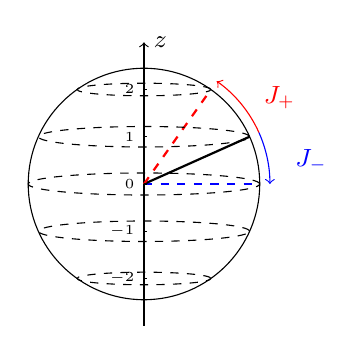
\begin{tikzpicture}
            \draw (0,0) circle (1.47);
            \draw[->] (0,-1.8)--(0,1.8)node[right]{\small\(z\)};
            \draw[blue,dashed,thick] (0,0)--(1.47,0);
            \draw[thick] (0,0)--(1.34,0.6);
            \draw[red,dashed,thick] (0,0)--(0.85,1.2);
            \draw[dashed] (0,0) ellipse (1.47 and 0.14);
            \draw[dashed] (0,0.6) ellipse (1.34 and 0.13);
            \draw[dashed] (0,1.2) ellipse (0.85 and 0.08);
            \draw[dashed] (0,-0.6) ellipse (1.34 and 0.13);
            \draw[dashed] (0,-1.2) ellipse (0.85 and 0.08);
            \foreach \x in {-2,...,2}{
                \draw (0,0.6*\x)node[left]{\tiny\(\x\)}--(0.04,0.6*\x);
            }
            \draw[->,red] (1.46,0.653) arc (24.1:54.7:1.6);
            \node[red] at (1.4,1.1)[right]{\small\(J_+\)};
            \draw[->,blue] (1.46,0.653) arc (24.1:0:1.6);
            \node[blue] at (1.8,0.3)[right]{\small\(J_-\)};
        \end{tikzpicture}
        \caption{\(\vb{J}\) eigenvectors for \(j=2\) states. Only the magnitude and the projection along the \(z\) axis is definite so each state is represented by a circle on a sphere. The raising and lowering operators makes the \(\vb{J}\) more/less aligned with the \(z\) axis.}
    \end{figure}

    \subsection{Rotations and Orientations}
    Note that, since \(J_x\) and \(J_y\) can be written in terms of the raising and lowering operators \(J_{\pm}\), rotations around an arbitrary axis transform states in a given \(\hb_j\) into other states in the same \(\hb_j\). Since \(J_x=(J_+ +J_-)/2\), we see that when \(j>0\), the state \(\ket{j,m}\) is never an eigenstate of \(J_x\). Hence, for \(j>0\), we can never be certain of the outcome of measurements of both \(J_x\) and \(J_z\). This argument applies equally to \(J_y\), so it's impossible to be certain of the outcome of measurements of more than one component of \(\vb{J}\). If \(j=0\), every component of \(\vb{J}\) yields zero, but a null vector in \(\RR^3\) has no direction. This situation contrasts with the momentum vector \(\vb{P}\) which can have well-defined direction since all its components commute with one another.

    In the mathematical literature, states with \(m=j\) are known as \textit{highest weight states}. They play a key role in the representation theory of any group \(G\), because once we know the highest weight state the rest of the multiplet can be constructed by applying lowering operators such as \(J_-\). Physically, a highest weight state is one in which the body's angular momentum is most nearly aligned along the \(z\)-axis. In this state, the ratio of the squared angular momentum that lies in the \(xy\)-plane to that parallel to the \(z\)-axis is
    \begin{equation}
        \frac{\expval{J_x^2+J_y^2}{j,j}}{\expval{J_z^2}{j,j}}=\frac{\expval{\vb{J}^2-J_z^2}{j,j}}{\hbar^2j^2}=\frac{1}{j}\,.
    \end{equation}
    As \(J_x=(J_+ + J_-)/2\) we have \(\expval{J_x}{j,j}=0\) and similarly \(\expval{J_y}{j,j}=0\). Thus we have no information about the direction in the \(xy\)-plane any angular momentum points.

    Macroscopic bodies, for which \(j\gg 1\), have only a tiny fraction of their total angular momentum in the \(xy\)-plane when they're in state \(\ket{j,j}\), so the uncertain direction of this component of angular momentum does not lead to significant uncertainty in the total direction of the angular momentum vector. By contrast, when \(j=1/2\), even in state\(\ket{1/2,1/2}\) there's twice as much angular momentum associated with the \(xy\)-plane as with the \(z\)-axis and the uncertain direction of this planar component makes it impossible to say anything more specific than that the angular momentum vector lies somewhere in the northern, rather than southern, hemisphere. Even when \(j=1\) and \(m=1\), the state \(\ket{1,1}\) has as much angular momentum along the \(xy\)-plane as it has parallel to the \(z\)-axis, so the direction of the angular momentum vector is still very uncertain. This is no surprise: since \(\dim(\hb_j)=2j+1\), when \(j=1/2\) there are only two independent states the orientation of our body can take. With such a limited Hilbert space it's no wonder we only have a fuzzy notion of where the body's angular momentum lies.

    \subsubsection{Rotations of Diatomic Molecules}
    Our deduction of the possible eigenvalues and eigenstates of \(\vb{J}^2\) and \(J_z\) came from considering rotations: the states \(\ket{j,m}\) simply enable us to describe what happens when an object is rotated around some axis, as we'll understand in more detail and with many examples later in the chapter. In particular, it's important to understand that \textit{a priori} these states have nothing to do with the energy levels of any given particle. As always, there's no way to tell how rotating an object may or may not change its energy until we specify a form for the Hamiltonian. In this section, we'll choose a simple form of dynamical relation \(H=H(\vb{J})\) that will enable us to understand an important part of the dynamics of a diatomic molecule.

    For some purposes, a diatomic molecules such as \(\mathrm{CO}\) molecule can be considered to consist of two point masses, the nuclei of the oxygen and carbon atoms, joined by a ``light rod'' provided by the electrons. Following the analogous formula in classical mechanics, we model the dynamics of this molecule by the Hamiltonian
    \begin{equation}
        H=\frac{1}{2}\left(\frac{J_x^2}{I_x}+\frac{J_y^2}{I_y}+\frac{J_z^2}{I_z}\right)\,,
    \end{equation}
    where \(I_x\) is the moment of inertia along the \(x\)-axis, and similarly for \(I_y\) and \(I_z\). Though motivated by classical mechanics, the best justification for this form of Hamiltonian is ultimately that it agrees with detailed experiments.

    \begin{figure}
        \centering
        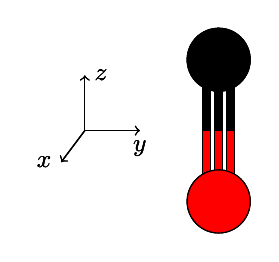
\begin{tikzpicture}
            \foreach \x in {0,1,2}{
                \draw[fill=black](0.15*\x,0) rectangle (0.1+0.15*\x,0.6);
                \draw[fill=red](0.15*\x,0) rectangle (0.1+0.15*\x,-0.6);
                \draw[fill=black] (0.2,0.9) circle (0.4);
                \draw[fill=red] (0.2,-0.9) circle (0.4);
                \draw[->] (-1.5,0)--(-1.5,0.7)node[right]{\small \(z\)};
                \draw[->] (-1.5,0)--(-0.8,0)node[below]{\small \(y\)};
                \draw[->] (-1.5,0)--(-1.8,-0.4)node[left]{\small\(x\)};
            }
        \end{tikzpicture}
        \caption{A simple model of carbon monoxide. By symmetry, \(I_x=I_y\) whilst \(I_z\) is much smaller.}
    \end{figure}

    In our axisymmetric case, we choose coordinates whose origin is at the centre of mass of the molecule (somewhere between the \(\mathrm{C}\) and \(\mathrm{O}\) atoms). Then \(I_x=I_y=I\), say, whilst \(I_z\) is different. In fact, since the centre of mass of the \(\mathrm{C}\) and \(\mathrm{O}\) atoms lies along the \(z\)-axis, the molecule's moment of inertia around this axis is negligible, \(I_z\ll I\). We can thus rewrite our Hamiltonian as
    \begin{equation}
        H=\frac{1}{2}\left[\frac{\vb{J}^2}{I}+J_z^2\left(\frac{1}{I_z}-\frac{1}{I}\right)\right]\,.
    \end{equation}
    The virtue of expressing \(H\) in terms of \(\vb{J}^2\) and \(J_z\) is that our knowledge of the spectrum of these operators immediately allows us to write down the spectrum of this Hamiltonian: the state \(\ket{j,m}\) is an energy eigenstate with
    \begin{equation}
        E_{jm}=\frac{\hbar^2}{2}\left[\frac{j(j+1)}{I}+m^2\left(\frac{1}{I_z}-\frac{1}{I}\right)\right]\,,
    \end{equation}
    with \(\abs{m}\le j\). Since \(I_z\ll I\) for our diatomic molecule, the coefficient of \(m^2\) is very much greater than that of \(j(j+1)\), so states with \(m\ne 0\) will only occur very far above the ground state. Consequently, the low lying states have energies of the form
    \begin{equation}
        E_j=\frac{\hbar^2}{2I}j(j+1)
    \end{equation}
    for some \(j\). As we saw in the previous section, only discrete values of \(j\) are allowed, so the energy levels are quantized. One can excite a \(\mathrm{CO}\) molecule, causing it to rotate faster, only by supplying a definite amount of energy. Similarly, for the molecule to relax down to a state of lower angular momentum, it must emit a quantized lump of energy.
    
    Carbon monoxide is a significantly dipolar molecule. The carbon atom has a smaller share of the binding electrons than does the oxygen, with the result that it is positively charged while the oxygen atom gains negative charge. In Maxwell's theory of electrodynamics, a rotating electric dipole is expected to emit electromagnetic radiation. Because we're in the quantum regime, this radiation emerges as photons which, as we'll see later in the chapter, can add or carry away only one unit \(\hbar\) of angular momentum. Thus the energies of the photons that can be emitted or absorbed by a rotating dipolar molecule are
    \begin{equation}
        E_\gamma=\pm(E_j-E_{j-1})=\pm\frac{j\hbar^2}{I}\,.
    \end{equation}
    Using the relation \(E=\hbar\omega\), the angular frequencies in the rotation spectrum of the molecule are
    \begin{equation}\label{diatomic_spectra}
        \omega_j=\frac{j\hbar}{I}\,.
    \end{equation}
    In the case of \(\mathrm{^{12}CO}\), \(\hbar/2\pi I\) evaluates to a frequency \(\nu\sim 115.271\unit{GHz}\) and spectral lines occur at multiples of this frequency. In the classical limit of large \(j\), the molecule's total angular momentum \(\abs{\vb{J}}\approx j\hbar\). This is related to the angular frequency \(\Omega\) at which the molecule rotates by \(\abs{\vb{J}}=I\Omega\). Comparing to (\ref{diatomic_spectra}) we see that in the classical limit, \(\omega_{j\gg 1}=\Omega\), so the frequency of the emitted radiation is just the frequency at which the molecule rotates.

    Measurements of the radiation at \(115.271\unit{GHz}\) provide one of the two most important probes of interstellar gas\footnote{The other key probe is the hyperfine line of atomic hydrogen that will be discussed in \cref{Chap:Time_Independent_Perturbation}.}. In denser, cooler regions, hydrogen atoms combine to form \(\mathrm{H_2}\) molecules which are centrosymmetric and do not have an electric dipole moment when they rotate. Consequently, these molecules, which together with similarly uncommunicative Helium make up the vast majority of cold interstellar gas, lack readily observable spectral lines. Astronomers are thus obliged to study the interstellar medium through the rotation spectrum of the few parts in a million of \(\mathrm{CO}\) it contains.

    \subsection{Spin}\label{Chap:Spin}
    We saw that the orbital angular momentum operator \(\vb{L}\) and spin operator \(\vb{S}\) each obey an identical algebra to that of the rotation generators
    \begin{align}
        [L_i,L_j]&=\ii\hbar\sum_k\epsilon_{ijk}L_k &[L_i,\vb{L}^2]&=0\\
        [S_i,S_j]&=\ii\hbar\sum_k\epsilon_{ijk}S_k &[S_i,\vb{S}^2]&=0
    \end{align}
    as well as \([S_i,L_j]=0\). Since the algebra of the \(\vb{J}\)'s was all we used to deduce their spectra, it follows immediately that \((\vb{L}^2,L_z)\) and \((\vb{S}^2,S_z)\) have the same possible spectra as we found for \((\vb{J}^2,J_z)\). It is conventional to label eigenstates of \((\vb{L}^2,L_z)\) as \(\ket{\ell,m}\) and those of \((\vb{S}^2,S_z)\) as \(\ket{s,\sigma}\), where \(\ell\) and \(s\) correspond to the eigenvalues of \(\vb{L}^2\) and \(\vb{S}^2\), respectively, and \(m\) and \(\sigma\) label the eigenvalues of \(L_z\) and \(S_z\). (Unfortunately, it's traditional to label the eigenvalue of both \(J_z\) and \(L_z\) by the same letter \(m\). Which is meant is usually clear from the context.)

    \subsubsection{Large Rotations}\label{Chap:Large_Rot}
    Our claim that the possible values for \((j,m)\) are
    \begin{equation}
        j\in\left\{0,\frac{1}{2},1,\frac{3}{2},\dots\right\}\qquad\text{and then}\qquad m\in\{-j,\dots,j-1,j\}
    \end{equation}
    was based on examining the algebra \([J_i,J_j]=\ii\hbar\sum_k\epsilon_{ijk}J_k\) and likewise for \((\ell,m_\ell)\) or \((s,\sigma)\). In turn, this algebra originally came from considering the behaviour of objects under very small rotations. We now check whether these spectra are also compatible with large rotations.

    Suppose we rotate the state \(\ket{j,m}\) through an amount \(\alpha\) around the \(z\)-axis. Then 
    \begin{equation}
        \ket{j,m}\longrightarrow U(\alpha\vu{z})\ket{j,m}=\ee^{\ii \alpha J_z/\hbar}\ket{j,m}=\ee^{-\ii m\alpha}\ket{j,m}
    \end{equation}
    since it is an eigenstate of \(J_z\). Rotations through \(2\pi\) around any axis return us to our starting point, so are equivalent to no rotation. Thus, for \(U(\bm{\alpha})\) to be a homomorphism from \(\SO(3)\) to the group of unitary operators on \(\hb\), we must have \(U(2\pi\vu{\alpha})=1_{\hb}\). In particular, when \(\vu{\alpha}=\vu{k}\), from above we must have \(\ee^{-2\pi \ii m}=1\). This is true if \(m\) is an integer, but not if it is an odd-half-integer. Since \(m\) is an integer or (odd) half-integer iff \(j\) is, we conclude that odd half-integer values of \(j\) are in fact not compatible with the behaviour of objects under large rotations: they are ruled out by our basic requirement that \(U(\vb{\alpha})\) represents the action of \(\SO(3)\) on \(\hb\).

    The fact that global properties of rotations rule out some of the eigenvalues allowed by the rotation algebra is an example of a phenomenon familiar from IB Methods. The behaviour of function in the neighbourhood of a point may be governed by some differential equation. The associated differential operator (if it's linear) typically has a large spectrum, which is cut down by boundary conditions or periodicity conditions. For example, on any open set \(U\subset\RR\) the linear operator \(-\ii\mathrm{d}/\mathrm{d}x\) has eigenfunctions \(\ee^{\ii kx}\) for any \(k\in\CC\). However, if we know that globally \(\psi:S^1\to\CC\) so is periodic, then \(k\) must be quantized in units of the circle's radius. The only difference in our case is that the non-trivial algebra of the rotation generators already restricted the possible eigenvalues of \(\vb{J}^2\) and \(J_z\) to be quantized in units of \(\hbar\). Global properties of the rotation group still remove some of the eigenvalues that were allowed locally. More succinctly, states where \(j\in\NN_0+\frac{1}{2}\) do form representations of the rotation algebra \(\mathfrak{so}(3)\), but not of the rotation group \(\SO(3)\).

    In fact, we'll see that our arguments above have been rather to hasty.

    \subsubsection{The Stern--Gerlach Experiment}\label{Chap:Stern_Gerlach}
    Quantization of angular momentum in units of \(\hbar\) was originally proposed by Bohr and Sommerfeld as a means by which the stability of atomic orbits could be understood; we've now seen how this quantization arises automatically in the full mathematical framework of quantum mechanics. However, back in 1922 it still seemed very mysterious, so Stern and Gerlach designed and conducted experiments to check whether angular momentum is really quantized in Nature.

    In the Stern--Gerlach experiments, a beam of uncharged atoms of the same type is passed through a region of slowly varying magnetic field. If the atoms have mass \(M\), the Hamiltonian for this process is\footnote{The potential energy resulting from coupling a magnetic dipole to an applied magnetic field is similar to the (perhaps more familiar) energy \(\vb{p}\vdot\vb{E}\) of an electric dipole \(\vb{p}\) in an applied electric field \(\vb{E}\). Note that the atoms carry no net electric charge, so there's no Lorentz force.}
    \begin{equation}
        H=\frac{\vb{P}^2}{2M}-\vb{\mu}\vdot\vb{B}\,,
    \end{equation}
    where \(\vb{B}\) is the applied magnetic field, and \(\vb{\mu}\) is the \textit{magnetic dipole moment} of the atom. Ultimately, the reason the atom can be treated as a magnetic dipole is because of detailed properties of the distribution of its electrons. It would take us too far afield to explain this precisely, but the dipole moment arises because the atom has an orientation: a perfectly spherically symmetric atom cannot have any dipole moment as there is no preferred direction for the ``north'' or ``south'' poles. Thus the dipole moment is only non-zero for atoms that transform non-trivially under \(\vb{S}\). If the atom is in the spin \(s\) representation, we can write \(\vb{\mu}=(\mu/\hbar s)\vb{S}\).

    \begin{figure}
        \centering
        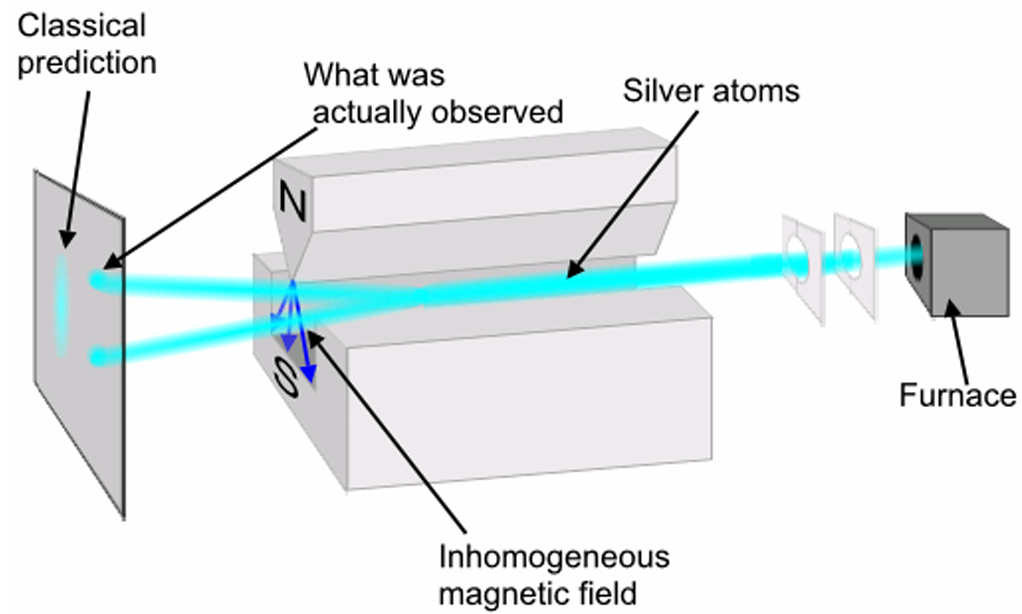
\includegraphics[width=0.6\textwidth]{Stern-Gerlach.png}
        \caption{A schematic picture of the Stern--Gerlach experiment, adapted from the Astronomy Cast site.}
    \end{figure}

    Choosing our coordinates so that the \(z\)-axis points along the direction of the magnetic field, the Hamiltonian becomes
    \begin{equation}
        H=\frac{\vb{P}^2}{2M}-\frac{\mu}{\hbar s}BS_z\,,
    \end{equation}
    where \(B=\abs{\vb{B}}\). The equations of motion obtained using the Heisenberg picture tell us that the expectation values of position and momentum in any state obey
    \begin{equation}
        \dv{}{t}\eval{\vb{X}}=\frac{\eval{\vb{P}}}{M}\quad\text{and}\quad\dv{}{t}\eval{\vb{P}}=\frac{\mu}{\hbar s}\eval{(\grad B)S_z}\,.
    \end{equation}
    The second of these equations is analogous to the classical \(\vb{F}=-\grad V\).

    We see that the force experienced by any given atom depends on its value of \(S_z\). For a spin \(s\) particle, these are \(\hbar\{-s,-s+1,\dots,s\}\) and in particular can be of either sign. If an atom is in the state \(\ket{s,s}\) with all its spin aligned along the direction of \(\vb{B}\), then it will experience a force pushing it in the direction of increasing magnetic field. On the other hand, those atoms in the state \(\ket{s,-s}\) will be pushed in the direction of decreasing \(B\), while atoms with \(\sigma=0\) (when \(s\) is an integer) are unaffected. In total, when an initial beam of atoms in which the spins are randomly aligned passes through the region of magnetic field, it will be split into \(2s+1\) different trajectories. Thus, if the atoms are perfectly spherical, they will pass through unaffected, whereas if they have \(s=1\) the beam will be split into three, corresponding to the three possible eigenvalues \(\{-\hbar,0,\hbar\}\), if they have \(s=2\) the beam will split into five, and so on. Finally, if the atoms have very large spin (and so a very definite orientation in space) the beam will be split into so many paths that we can no longer distinguish the individual paths, seeing instead a broad smear. This is the same result we'd expect to find if angular momentum is not quantised, where the amount by which an atom is deflected would depend smoothly on its orientation with respect to \(\vb{B}\).

    Stern and Gerlach's original experiment in fact used silver atoms. Their magnetic was controlled by a dial. Initially, as \(B=0\) the atoms all passed straight through. As they turned up the magnetic field, the beam split into \textbf{two} separate paths. As \(\vb{B}\) was further increased, the separation between these two beams increased, but no further splitting was observed. Thus, not only is angular momentum quantized as Bohr and Sommerfeld had predicted, but silver atoms have spin \(s=\frac{1}{2}\)!
    \subsubsection{Spinors and Projective Representation (Non-examinable)}
    The Stern--Gerlach experiment shows that, despite our arguments, half integer values of \(s\) actually arise in Nature. In fact, the chemical properties of the elements and the structure of the periodic table, together with properties of materials such as metals, conductors and insulators depends crucially on particles having half-integer values of spin. These values are in conflict with our current mathematical formalism, so we must have made a mistake, imposing too strong a condition that ruled out the possibility of half-integer spins.

    The error lay in our claim that we needed to represent the action a transformation group \(G\) on Hilbert space \(\hb\), rather than just on projective Hilbert space \(\ph\). (Recall that states which differ only by an overall constant --- which does not need to have modulus \(1\) provided we use the general form of the Born rule --- yield the same results in all experiments. Thus physical systems are represented by states in projective Hilbert space.) Projectively, it's enough to require
    \begin{equation}\label{projective_homomorphism}
        U(g_2)\circ U(g_1)=\ee^{\ii \phi(g_2,g_1)}U(g_2\cdot g_1)
    \end{equation}
    rather than the homomorphism condition (\ref{homomorphism}), where \(\phi(g_1,g_2)\) is a real phase. This phase does not affect which ray in \(\hb\) the state lies in, so leaves the physics unchanged. The operator algebra is associative, so we must have
    \begin{equation}
        U(g_3)\circ(U(g_2)\circ U(g_1))=(U(g_3)\circ U(g_2))\circ U(g_1)\,,
    \end{equation}
    which implies the phase obey
    \begin{equation}\label{cocycles_condition}
        \phi(g_2,g_1)+\phi(g_3,g_2\cdot g_1)=\phi(g_3,g_2)+\phi(g_3\cdot g_2,g_1)\,.
    \end{equation}
    Phase factors \(\ee^{\ii \phi(g_2,g_1)}\) obeying this condition are known as \textit{cocycles} on the group \(G\). One possible solution of (\ref{cocycles_condition}) is to take
    \begin{equation}
        \phi(g_2,g_1)=\beta(g_2\cdot g_1)-\beta(g_2)-\beta(g_1)
    \end{equation}
    for arbitrary smooth function \(\beta:G\to\RR\). This solution is ``trivial'', because if \(\phi(g_2,g_1)\) takes this form, then we can define a new unitary transformation operator \(U'(g)=\ee^{\ii \beta(g)}U(g)\) which obeys our original condition (\ref{homomorphism}). By agreeing to work with the new operator, the phases never arise. The interesting question is whether there are other, non-trivial solutions to (\ref{cocycles_condition}).

    A theorem in group cohomology\footnote{Unfortunately, we won't prove this here. If you're interested, you can find a proof (given in the context of quantum mechanics) in either Weinberg's \textit{The Quantum Theory of Fields}, vol. 1 (chapter 2, appendix B), or else in Hall's \textit{Quantum Theory for Mathematicians}.} states that it is possible for non-trivial projective representations to arise for groups that are not simply connected\footnote{There's one other possibility: that the Lie algebra \(\mathfrak{g}\) contains central elements (vectors \(e\in\mathfrak{g}\) s.t. \([e,\mathfrak{g}]=0\)) that cannot be removed by a redefinition of the generators. This case is not relevant for us.}. In fact, this is the case for \(\SO(3)\). The topology of the rotation group can be seen by viewing each rotation as parameterised by a vector \(\vb{\alpha}\). If we allow the axis of rotation \(\vu{\alpha}\) to point in any direction, then rotations with \(\abs{\vb{\alpha}}\in(0,\pi)\) are uniquely specified. However, when rotating through \(\pi\) we get the same rotation whether rotating around \(\vu{\alpha}\) or \(-\vu{\alpha}\). Thus, we can picture the space of all rotations as a solid, three-dimensional ball \(\abs{\vb{\alpha}}\le\pi\), but with antipodal points on the surface \(\abs{\bm{\alpha}}=\pi\) identified the same.

    The description show that \(\SO(3)\) contains smooth, closed paths, beginning and ending at the identity rotation (the origin of the 3-ball) that cannot be continuously shrunk to a point. For example, consider the loops in \cref{Fig:SO3} which all start and end at the identity rotation, i.e.
    the centre of the sphere. Figure (i) shows a loop which is contractible; it can obviously be shrunk to a point. On the other hand, figure (ii) shows a loop for which the angle of rotation all starts at zero, smoothly increasing to \(\pi\) at the point \(A\). At this point it reaches the boundary and reappears at the antipodal point \(A'\), before continuing to increase to \(2\pi\) back at the identity. It should be intuitively clear that this loop cannot be shrunk to a point whilst keeping both its ends fixed at the identity.


    Next, consider the loop in figure (iii), along which the angle of rotation increases from \(0\) to \(4\pi\), reaching the boundary of the ball twice, once at \(A\), reappearing at \(A'\) and then again at \(B\) reappearing at \(B'\). By moving the two antipodal pairs, the section of the path between \(A'\) and \(B\) can be pulled across the boundary, smoothly deforming the loop back to the situation as in figure (i). Thus, after two complete rotations the situation becomes simple once more. In general, the angle along any closed path must increase by an integer multiple of \(2\pi\). The resulting loop will be contractible if this integer is even, but non-contractible if it is odd.
    
    \begin{figure}
        \centering
        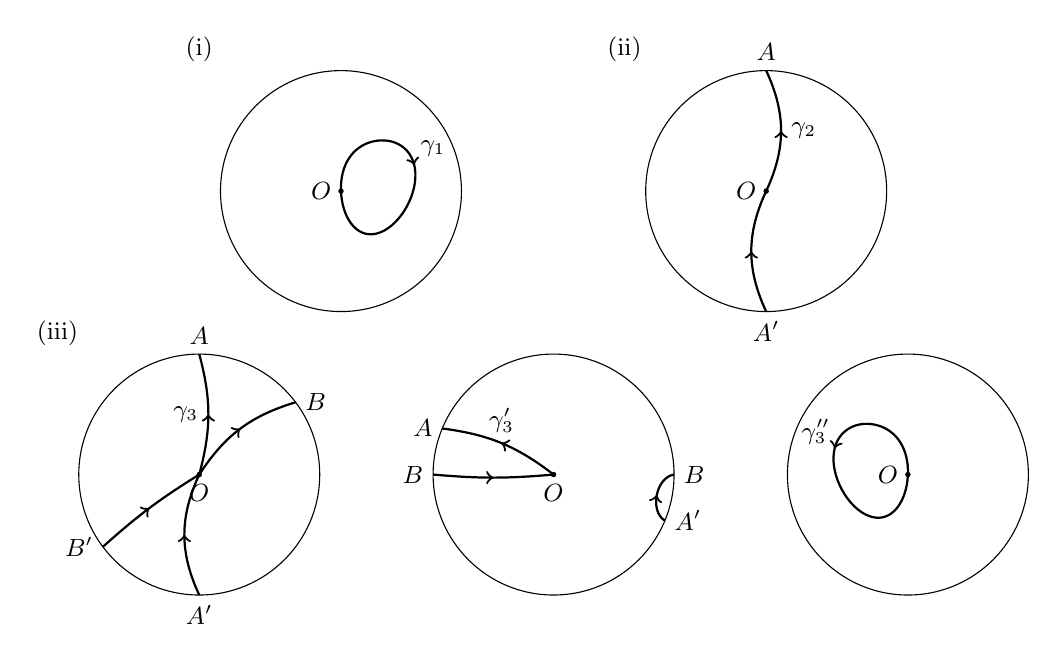
\begin{tikzpicture}[scale=0.9]
            \node at (-2,2) {\small(i)};
            \draw (0,0) circle (1.7);
            \draw[fill=black] (0,0) circle (0.03) node[left]{\small \(O\)};
            \draw[thick,decoration={markings, mark=at position 0.2 with {\arrow{>}}},postaction={decorate}] plot[smooth cycle, tension=1] coordinates{(0,0) (0.45,0.7)(1.05,0.25) (0.5,-0.6)};
            \node at (1.3,0.6) {\small \(\gamma_1\)};

            \node at (4,2) {\small(ii)};
            \draw (6,0) circle (1.7);
            \draw[fill=black] (6,0) circle (0.03) node[left]{\small \(O\)};
            \draw[thick,decoration={markings, mark=at position 0.5 with {\arrow{>}}},postaction={decorate}] (6,0) to [bend right=25] node[right]{\small \(\gamma_2\)}(6,1.7);
            \draw[thick,decoration={markings, mark=at position 0.5 with {\arrow{>}}},postaction={decorate}] (6,-1.7) to [bend left=25] (6,0);
            \node at (6,1.7)[above]{\small\(A\)};
            \node at (6,-1.7)[below]{\small\(A'\)};

            \node at (-4,-2) {\small(iii)};
            \draw (-2,-4) circle (1.7);
            \draw[fill=black] (-2,-4) circle (0.03) node[below]{\small \(O\)};
            \draw[thick,decoration={markings, mark=at position 0.5 with {\arrow{>}}},postaction={decorate}] (-2,-4) to [bend right=15] node[left]{\small \(\gamma_3\)}(-2,-2.3);
            \draw[thick,decoration={markings, mark=at position 0.5 with {\arrow{>}}},postaction={decorate}] (-2,-5.7) to [bend left=25] (-2,-4);
            \draw[thick,decoration={markings, mark=at position 0.5 with {\arrow{>}}},postaction={decorate}] (-2,-4) to [bend left=20] (-0.64,-2.98);
            \draw[thick,decoration={markings, mark=at position 0.5 with {\arrow{>}}},postaction={decorate}] (-3.36,-5.02) to [bend left=5] (-2,-4);
            \node at (-2,-2.3)[above]{\small\(A\)};
            \node at (-2,-5.7)[below]{\small\(A'\)};
            \node at (-0.64,-2.98)[right]{\small\(B\)};
            \node at (-3.36,-5.02)[left]{\small\(B'\)};


            \draw (3,-4) circle (1.7);
            \draw[fill=black] (3,-4) circle (0.03) node[below]{\small \(O\)};
            \draw[thick,decoration={markings, mark=at position 0.5 with {\arrow{>}}},postaction={decorate}] (3,-4) to [bend right=15] node[above]{\small \(\gamma_3'\)}(1.43,-3.35);
            \draw[thick,decoration={markings, mark=at position 0.5 with {\arrow{>}}},postaction={decorate}] (4.57,-4.65) to [bend left=70] (4.7,-4);
            \draw[thick,decoration={markings, mark=at position 0.5 with {\arrow{>}}},postaction={decorate}] (1.3,-4) to [bend right=5] (3,-4);
            \node at (4.7,-4)[right]{\small\(B\)};
            \node at (1.3,-4)[left]{\small\(B\)};
            \node at (1.43,-3.35)[left]{\small\(A\)};
            \node at (4.57,-4.65)[right]{\small\(A'\)};


            \draw (8,-4) circle (1.7);
            \draw[fill=black] (8,-4) circle (0.03) node[left]{\small \(O\)};
            \draw[thick,decoration={markings, mark=at position 0.2 with {\arrow{>}}},postaction={decorate}] plot[smooth cycle, tension=1] coordinates{(8,-4) (7.55,-3.3)(6.95,-3.75) (7.5,-4.6)};
            \node at (6.7,-3.4) {\small \(\gamma_3''\)};
        \end{tikzpicture}
        \caption{Paths in \(\SO(3)\) (i) contractible (ii) a loop with angles increasing by \(2\pi\) that is non-contractible (iii) a loop with angles increased by \(4\pi\) but it is again contractible.}
        \label{Fig:SO3}
    \end{figure}

    The topological properties of paths in \(G\) become important when we consider the behaviour of \(U(g)\) as the group element \(g\) varies around a loop \(L\), beginning and ending at some fixed \(g_0\). It is quite possible for \(U(g)\) to change smoothly with \(g\) along \(L\) in such a way that the operators at each end of the loop do not coincide: they may differ by a phase
    \begin{equation}
        U(g_0)\xlongrightarrow{L}\alpha_L U(g_0)\,,
    \end{equation}
    where the phase \(\alpha_L\) depends on the loop. This is consistent with the projective homomorphism (\ref{projective_homomorphism}).

    To investigate the possibilities for \(\alpha_L\), let's specialize to the case in which the operators act on a Hilbert space of finite dimension \(N\), so that each \(U(g)\) can be regarded as an \(N\times N\) unitary matrix. We can use up some of the freedom in (\ref{projective_homomorphism}) by requiring that each such matrix has unit determinant. This does not fix things completely, but the residual freedom is discrete:
    \begin{equation}
        \det U(g)=+1\ \forall g\in G\implies \ee^{\ii N\phi(g_1,g_2)}=1\,.
    \end{equation}
    If \(G\) is simply connected, meaning that any closed loop is contractible, then the determinant condition implies \(\alpha_L=1\) for all loops \(L\). This follows straightforwardly using continuity: \(\alpha_L\) must be an \(N^{\text{th}}\) root of unity, but if it varies continuously as we vary our loop \(L\) and if all such loops are contractible to the single point \(g_0\), then we must have the same matrix at the beginning and ending of each loop, so \(\alpha_L=1\).
    
    If G is not simply connected, the same argument still shows that \(\alpha_L=1\) for any contractible \(L\), but there may also be non-contractible loops with \(\alpha_L\ne 1\). In this case, we can at least deduce that \(\alpha_L=\alpha_{L'}\) whenever the loops \(L\) and \(L'\) are in the same homotopy class, meaning that they can be smoothly deformed into one another. Furthermore, if loops \(L\) and \(L'\) are traversed successively, then \(U(g_0)\xleftarrow{L}\alpha_L U(g_0)\xleftarrow{L'}\alpha_L\alpha_{L'}U(g_0)\), so there are self-consistency constraints.

    We can now give a unique definition of \(U(g)\) for all \(g\) in a simply connected Lie group \(G\). Recalling that \(U(e)=\Id_\hb\), we define \(U(g_0)\) by choosing any path from the identity \(e\) to \(g_0\) and demanding that \(U(g)\) changes smoothly along this path. The values along the path are unique by the determinant and continuity conditions, but the end result \(U(g_0)\) is also unique, because by traversing them in opposite directions, any two paths \(e\to g_0\) can be combined to form a closed loop at \(g_0\). This loop is contractible since our group is simply connected. With this definition, continuity also ensures that all cocycles are equal to one, so we have a genuine representation (not just a projective representation) of \(G\).

    Carrying out the same construction when \(G\) is not simply connected, we'll encounter paths from \(e\) to \(g_0\) which cannot be smoothly deformed into one another. Thus, starting from \(U(e)=\Id_\hb\), in general we obtain different values for \(U(g_0)\) depending on the path we take. In this way we're forced to consider multi-valued functions on \(G\) (just as when defining a continuous square root in the complex plane). The ambiguity, or multi-valuedness, in \(U(g_0)\) can be resolved only by keeping track of the path we used to reach \(g_0\), just as for the complex square root we must keep track of how many times we've encircled the origin to be sure which branch we're on. Such a multi-valued definition inevitably means that non-trivial cocyles appear.

    As we saw above, the rotation group \(G=\SO(3)\) is not simply connected, but there are just two topological classes of loops, depending on whether the net angle of rotation is an even or odd multiple of \(2\pi\). Any loop \(L\) in the first class is contractible and so has \(\alpha_L=1\). Any loop \(L\) in the second class is non-contractible, but if we traverse \(L\) twice it becomes contractible again. Thus \(\alpha_{L'}^2=1\) and \(L=\pm 1\). The finite-dimensional spaces \(\hb_j\) on which the rotation operators act are nothing but the multiplets of total angular momentum \(j(j+1)\hbar^2\), with a basis \(\ket{j,m}\) where
    \begin{equation}
        m\in\{-j,-j+1,\dots,j-1,j\}\,.
    \end{equation}
    Thus \(\dim\hb_j=2j+1\). From the determinant condition \((\alpha_L)^{2j+1}=1\) for any loop, but our topological considerations \(\alpha_L=\pm 1\). If \(j\) is an integer then \(2j+1\) is odd and it follows that \(\alpha_L=1\) for all loops, contractible or not. However, if \(j\) is an odd half-integer, then \(2j+1\) is even and \(\alpha_L=-1\) is possible for non-contractible loops. This is exactly the behaviour we found above: under the rotation operator \(U(\alpha\hat{\vb{z}})=\ee^{-\ii \alpha J_z/\hbar}\), a generic state in the \(j\) multiplet transforms as
    \begin{equation}
        \ket{\psi}=\sum_{m=-j}^{j}c_m\ket{j,m}\longmapsto U(\bm{\alpha})\ket{\psi}=\sum_{m=-j}^{j}c_m \ee^{-\ii \alpha m}\ket{j,m}\,.
    \end{equation}
    Any state with \(j\) (and hence all \(m\)) odd-half-integral changes sign under a rotation through an odd multiple of \(2\pi\). The discussion of this section shows that the origin of this unexpected sign is the non-trivial topology of the rotation group --- in our new terminology, we have a projective representation of \(\SO(3)\). These projective representations play an important role in physics, and are often called \textit{spinors}.

    We have, finally, obtained the correct mathematical framework in which to describe rotations and angular momentum in quantum mechanics. The history of the subject developed rather differently from the exposition we've given here. By the 1920's, careful studies of atomic spectroscopy had revealed that many spectral lines were in fact doubled, composed of two lines, very close in frequency. In 1924 (even before Schr\"{o}dinger published his famous equation) Pauli proposed that this doubling indicated that, in addition to the quantum numbers \(n,\ell,m\) labelling their energy levels, electrons possessed a further quantum number that took just two values. A year later, Uhlenbeck and Goudsmit suggested that this could be associated with some form of internal angular momentum. Their idea was initially treated with suspicion. If one wished to suppose the electron was a small, rotating sphere, then for it to have the needed angular momentum \(\hbar/2\) and yet keep its radius small enough so that its finite size would not have been detected by experiment\footnote{To date, no experiment has ever detected a finite size, or any other non-trivial internal spatial structure in the electron.}, the surface of the sphere would need to be travelling faster than light.

    Nevertheless, the Stern--Gerlach experiment showed that particles could indeed have spin, contributing to the Hamiltonian in the presence of a magnetic field in just the same way as would a classical spinning magnetic dipole. Heisenberg, Jordan and C. G. Darwin then showed that the internal spin of the electron exactly accounted for the fine splitting of spectral lines that had puzzled Pauli, as we'll see in \cref{Chap:Hydrogen_Fine_Structure}.

    We now understand that spin is an intrinsic property of fundamental particles: the Hilbert space of a fundamental particle is not simply \(H_{\text{spat}}=L^2(\RR^3,\d[3]{x})\) describing its spatial wavefunction, but rather a tensor product \(H_{\text{spat}}\otimes H_s\). However we may excite, crash into, or generally interfere with the motion of an electron or W boson, for as long as they remain electrons and W bosons, their spin will always be \(s=\frac{1}{2}\) and \(s=1\), respectively.

    \subsubsection{Spin Matrices}
    Since \(\sigma\in\{-s,-s+1,\dots,s-1,s\}\), states of definite total spin \(s\) can be described by a finite dimensional Hilbert space \(H_s\cong\CC^{2n+1}\). As always, once we pick a basis on \(\hb\) we can describe the action of linear operators such as \(\vb{S}\) explicitly in terms of matrices. Let's now carry this out the first few spin representations, working in the basis \(\{\ket{s,\sigma}\}\) of eigenstates of \(S_z\).

    The simplest case is \(s=0\), for which the only possible value of \(\sigma\) is also zero. This state obeys \(\ee^{-\ii \vb{\alpha}\vdot\vb{S}/\hbar}\ket{0,0}=\ket{0,0}\) for any \(\ket{\alpha}\). Hence a spin-zero object, like a perfect sphere, is completely unchanged under any rotation. In view of this, spin-zero particles are known as \textit{scalar particles}. The discovery of the Higgs boson, announced on \(4^{\text{th}}\) July 2012 at CERN in Geneva, was the first time a fundamental scalar particle had been observed in Nature.

    The next case is \(s=\frac{1}{2}\). Electrons, neutrinos and quarks are fundamental particles of spin \(\frac{1}{2}\), whilst protons, neutrons and the silver atoms used by Stern and Gerlach are examples of composite spin-half particles. When \(s=\frac{1}{2}\), \(\sigma\) can only take one of the two values \(\pm\frac{1}{2}\). For shorthand, we let \(\ket{\uparrow}\) denote the state \(\ket{s,\sigma}=\ket{\frac{1}{2},\frac{1}{2}}\) and \(\ket{\downarrow}\) denote \(\ket{\frac{1}{2},-\frac{1}{2}}\). A generic state of a spin-half system can thus be expanded as
    \begin{equation}
        \ket{\psi}=a\ket{\uparrow}+b\ket{\downarrow}
    \end{equation}
    in this basis, where \(a,b\in\CC\) and \(\abs{a}^2+\abs{b}^2=1\) so that \(\ket{\psi}\) is correctly normalised.

    In this basis, we can write the spin operators themselves as the \(2\times 2\) matrices
    \begin{align}
        S_{x}&=\begin{pmatrix}
            \mel{\uparrow}{S_x}{\uparrow} & \mel{\uparrow}{S_x}{\downarrow} \\
            \mel{\downarrow}{S_x}{\uparrow} & \mel{\downarrow}{S_x}{\downarrow}
        \end{pmatrix}\\
        S_y&=\begin{pmatrix}
            \mel{\uparrow}{S_y}{\uparrow} & \mel{\uparrow}{S_y}{\downarrow} \\
            \mel{\downarrow}{S_y}{\uparrow} & \mel{\downarrow}{S_y}{\downarrow}
        \end{pmatrix}\\
        S_z&=\begin{pmatrix}
            \mel{\uparrow}{S_z}{\uparrow} & \mel{\uparrow}{S_z}{\downarrow} \\
            \mel{\downarrow}{S_z}{\uparrow} & \mel{\downarrow}{S_z}{\downarrow}
        \end{pmatrix}\,.
    \end{align}
    Since \(\ket{\uparrow}\) and \(\ket{\downarrow}\) are eigenstates of \(S_z\), evaluating \(S_z\) in this basis is immediate. To also evaluate \(S_x\) and \(S_y\), we note that \(S_x=(S_+ + S_-)/2\) and \(S_y=(S_+ - S_-)/2\ii\) where \(S_\pm\) are the spin raising and lowering operators defined just as for \(J_\pm\). Using (\ref{ang_momentum_raising}) and (\ref{ang_momentum_lowering}) with \(j=s=\frac{1}{2}\) gives \(S_+\ket{\downarrow}=\hbar\ket{\uparrow}\) and \(S_-\ket{\uparrow}=\hbar\ket{\downarrow}\). In this way, we obtain
    \begin{equation}
        S_x=\frac{\hbar}{2}\begin{pmatrix}
            0 & 1 \\ 1 & 0
        \end{pmatrix}\,,\quad S_y=\frac{\hbar}{2}\begin{pmatrix}
            0 & -\ii \\ \ii & 0
        \end{pmatrix}\,,\quad S_z=\frac{\hbar}{2}\begin{pmatrix}
            1 & 0 \\ 0 & -1
        \end{pmatrix}\,.
    \end{equation}
    The coefficients for \(\hbar/2\) here are known as the \textit{Pauli matrices} and usually written as \((\sigma_x,\sigma_y,\sigma_z)\). Thus, for \(s=\frac{1}{2}\), we can write \(\vb{S}=\frac{\hbar}{2}\vb{\sigma}\).

    Proceeding to spin-one, we find three possible values \(\sigma\in\{-1,0,1\}\). Thus the spin-one Hilbert space is three (complex) dimensional, and when \(s=1\) we can represent each component of \(\vb{S}\) by a \(3\times 3\) matrix. In this case, the spin raising and lowering operators \(S_\pm\) act as
    \begin{equation}
        \begin{aligned}
            S_+\ket{1,-1}&=\sqrt{2}\hbar\ket{1,0}\qquad & S_+\ket{1,0}&=\sqrt{2}\hbar\ket{1,+1}\\
            S_-\ket{1,+1}&=\sqrt{2}\hbar\ket{1,0}\qquad & S_-\ket{1,0}&=\sqrt{2}\hbar\ket{1,-1}\,.
        \end{aligned}
    \end{equation}
    Using this result, one can check that
    \begin{equation}
        S_x=\frac{\hbar}{\sqrt{2}}\begin{pmatrix}
            0 & 1 & 0 \\
            1 & 0 & 1 \\
            0 & 1 & 0
        \end{pmatrix}\,,\quad S_y=\frac{\hbar}{\sqrt{2}}\begin{pmatrix}
            0 & -\ii & 0 \\
            \ii & 0 & -\ii \\
            0 & \ii & 0
        \end{pmatrix}\,,\quad S_z=\hbar\begin{pmatrix}
            1 & 0 & 0 \\
            0 & 0 & 0 \\
            0 & 0 & -1
        \end{pmatrix}\,.
    \end{equation}
    Sadly, these matrices don't have any special name. Examples of fundamental particles with spin-one are the somewhat unimaginatively named W and Z bosons\footnote{Although the photon carries one unit of \(\hbar\) in intrinsic angular momentum, it has only two possible states corresponding to left- or right- circular polarized light. Because the photon is massless, one needs to consider representations of the Lorentz group, rather than the spatial rotation group, in order to describe it accurately. We won't do this in this course.}. These are responsible for the weak interactions that, among other things, allows two hydrogen nuclei to fuse into Deuterium, powering nuclear fusion in the core of stars.

    In just the same way, we can represent each component of the spin operator by a \((2s+1)\times (2s+1)\) matrix for any finite \(s\). Since our basis is adapted to \(S_z\), the matrix representation of \(S_z\) will be
    \begin{equation}
        S_z=\hbar\diag(s,s-1,\dots,-s+1,-s)\,.
    \end{equation}
    Matrices for \(S_x\) and \(S_y\) may be constructed using the spin raising and lowering operators as above. Since \(S_\pm\) only change the \(z\)-component of the spin by 1 unit, these matrices are very sparse. One finds that they have non-zero entries only along the subleading diagonals, given by
    \begin{equation}
        \begin{aligned}
            (S_x)_{\sigma'\sigma}&=\frac{\hbar}{2}[\alpha(\sigma)\delta_{\sigma'-1,\sigma}+\alpha(\sigma-1)\delta_{\sigma'+1,\sigma}]\\
            (S_y)_{\sigma'\sigma}&=\frac{\hbar}{2\ii}[-\alpha(\sigma)\delta_{\sigma'-1,\sigma}+\alpha(\sigma-1)\delta_{\sigma'+1,\sigma}]\,,
        \end{aligned}
    \end{equation}
    where \(\alpha(\sigma)=\sqrt{(s-\sigma)(s+\sigma+1)}\). Note that, whatever the value of \(s\), we always have three matrices \((S_x,S_y,S_z)\) describing reorientations around the three independent axes in \(\RR^3\). Note also that each of these matrices is indeed traceless, as required by \(\ii\hbar\epsilon_{ijk}\tr_\hb(S_k)=\tr_\hb([S_i, S_j])=0\) as we said at the beginning of the chapter.

    In elementary particle physics (and also in Tripos questions), one rarely encounters spins higher than 1. Nonetheless, it's interesting to consider the limits \(s\gg 1\) of very high spins to see how our classical intuition emerges. For example, an electric motor that is roughly \(1\unit{cm}\) in diameter and weighs about \(10\unit{g}\) might spin at \(\sim 100\) revolutions per second. Its intrinsic angular momentum is then \(10^3\unit{kg}\unit{m}^2\unit{s}^{-1}\approx 10^31\hbar\). The classical world thus involves huge values of \(s\).

    Let's now show that, when \(s\gg 1\), there is very little uncertainty in the direction of a system's spin. Suppose our system is in the state \(\ket{s,s}\) so that its spin in maximally aligned with the \(z\)-axis. Let's compute \(\expval{\vb{n}\vdot\vb{S}}{s,s}\) where \(\vb{n}=(\sin\theta,0,\cos\theta)\). That is, we want to know how much spin we expect to measure along a direction in the \(xz\)-plane, inclined at angle \(\theta\) to the \(z\)-axis. Classically this would just be \(\hbar s\cos\theta\), the projection of \(\hbar s\) onto this axis. Quantum mechanically, we have
    \begin{equation}
        \expval{\vb{n}\vdot\vb{S}}{s,s}=\sin\theta\expval{S_x}{s,s}+\cos\theta\expval{S_z}{s,s}=\hbar s\cos\theta
    \end{equation}
    using the fact that \(S_x=(S_+ + S_-)/2\). Thus, on average the quantum result agrees with the classical intuition. This holds for any value of \(s\), but now let's ask what the uncertainty in this result is. We compute
    \begin{align}
        \expval{(\vb{n}\vdot\vb{S})^2}{s,s}&=\sin^2\theta\expval{S_x^2}{s,s}+\sin\theta\cos\theta\expval{S_xS_z+S_zS_x}{s,s}+\cos^2\theta\expval{S_z^2}{s,s}\notag\\
        &=\frac{1}{4}\sin^2\theta\expval{s,s}{S_+S_-}{s,s}+\hbar^2 s^2\cos^2\theta\notag\\
        &=\hbar^2\left(\frac{s}{2}\sin^2\theta+s^2\cos^2\theta\right)\,,
    \end{align}
    with all other terms vanishing. Consequently
    \begin{equation}
        \sqrt{\eval{(\vb{n}\vdot\vb{S})^2}-\eval{\vb{n}\vdot\vb{S}}^2}=\sqrt{\frac{s}{2}}\hbar\abs{\sin\theta}
    \end{equation}
    and so, in the classical limit of large \(s\), the relative uncertainty is small compared to \(\eval{\vb{n}\vdot\vb{S}}\) (ratio \(\sim\sqrt{\frac{1}{s}}\)).

    \subsubsection{Paramagnetic Resonance and MRI Scanners}
    In the presence of an external magnetic field, a classical magnetic dipole \(\vb{\mu}\) experiences a torque
    \begin{equation}
        \dv{\vb{L}}{t}=\vb{\mu}\cross\vb{B}\,.
    \end{equation}
    The dipole will thus turn until it aligns itself along the direction of the field, minimizing its energy. This is familiar from a compass. However, suppose the dipole is already spinning around its centre of mass, such that \(\vb{\mu}=\gamma\vb{L}\) where the constant \(\gamma\) is known as the gyromagnetic ratio. Then instead one finds that the torque causes the dipole to precess around \(\vb{B}\).

    As in our discussion of the Stern--Gerlach experiment, particles such as a proton or electron do have magnetic dipole moments \(\vb{\mu}=(2\mu/\hbar)\vb{S}\) proportional to their spin. We'll see that in quantum mechanics, this spin does indeed precess around the direction of an applied magnetic field. This is the basis of MRI scanners, which have become an enormously important diagnostic tool for both chemistry and medicine.

    We can understand the basic principles of an MRI machine by using our spin matrices. Unlike the beam of silver atoms in the Stern--Gerlach experiment, here the protons are not free to move, because they're held in place by the electromagnetic binding forces of a complex molecule, and this molecule is also held in a (roughly) fixed place in our cells. Thus we take the Hamiltonian to be
    \begin{equation}
        H=-\vb{\mu}\vdot\vb{B}=-\frac{2\mu B}{\hbar}S_z\,,
    \end{equation}
    with no kinetic term. Again, we've chosen the direction of the magnetic field to define the \(\vu{z}\) axis. In particular, for a spin-\(\frac{1}{2}\) particle such as a proton, the eigenvalues of this Hamiltonian are \(E_\pm=\mp\mu B\), where \(B=\abs{\vb{B}}\).

    Initially, we cannot expect the protons in our body to have their spins already aligned along \(\vb{B}\). Suppose instead that some proton has its spin aligned along some axis \(\vb{n}=(0,\sin\theta,\cos\theta)\) inclined at angle \(\theta\) to \(\vb{B}\). That is, we consider a proton in the state \(\ket{\theta_{\uparrow}}\) defined by
    \begin{equation}\label{MRI_theta_state}
        \vb{n}\vdot\vb{S}\ket{\theta_{\uparrow}}=\frac{\hbar}{2}\ket{\theta_{\uparrow}}\,.
    \end{equation}
    We can always choose to expand this state in terms of our basis \(\{\ket{\uparrow},\ket{\downarrow}\}\), representing states of definite spin along \(\hat{\vb{z}}\), as
    \begin{equation}
        \ket{\theta_{\uparrow}}=a\ket{\uparrow}+b\ket{\downarrow}\,,
    \end{equation}
    where \(\abs{a}^2+\abs{b}^2=1\). In terms of our Pauli matrices, the eigenvalue equation (\ref{MRI_theta_state}) becomes
    \begin{equation}
        \frac{\hbar}{2}\sin\theta\begin{pmatrix}
            0 & -\ii \\ \ii & 0
        \end{pmatrix}\begin{pmatrix}
            a \\ b
        \end{pmatrix}+\frac{\hbar}{2}\cos\theta\begin{pmatrix}
            1 & 0 \\ 0 & -1
        \end{pmatrix}\begin{pmatrix}
            a \\ b
        \end{pmatrix}=\frac{\hbar}{2}\begin{pmatrix}
            \cos\theta & -\ii\sin\theta \\
            \ii\sin\theta & -\cos\theta
        \end{pmatrix}\begin{pmatrix}
            a \\ b
        \end{pmatrix}=\frac{\hbar}{2}\begin{pmatrix}
            a \\ b
        \end{pmatrix}\,.
    \end{equation}
    Solving this eigenvalue problem and the normalisation condition yields \(a=\cos\frac{\theta}{2}\) and \(b=\ii\sin\frac{\theta}{2}\) (up to a possible phase), so a proton whose spin is aligned along the \(\vb{n}\) axis is in the state
    \begin{equation}
        \ket{\theta_\uparrow}=\cos\frac{\theta}{2}\ket{\uparrow}+\ii\sin\frac{\theta}{2}\ket{\downarrow}\,.
    \end{equation}
    Note that \(\ket{\theta_\uparrow}\) has the expected behaviour at \(\theta=0\) and \(\theta=\pi\), and it yields \(-\ket{\uparrow}\) as \(\theta\) is continuously increased to \(2\pi\). (It's straightforward to generalised this example to the case of a state with spin aligned along an arbitrary axis \(\vb{n}\).)

    Applying the time evolution operator \(U(t)=\ee^{-\ii Ht/\hbar}\), we find that at time \(t\) the proton's state has evolved to
    \begin{align}
        \ket{\psi(t)}&=U(t)\ket{\theta_\uparrow}=\cos\frac{\theta}{2}\ee^{-\ii Ht/\hbar}\ket{\uparrow}+\ii\sin\frac{\theta}{2}\ee^{-\ii Ht/\hbar}\ket{\downarrow}\notag\\
        &=\cos\frac{\theta}{2}\ee^{-\ii \omega t/2}\ket{\uparrow}+\ii\sin\frac{\theta}{2}\ee^{+\ii \omega t/2}\ket{\downarrow}\,,
    \end{align}
    where \(\omega=2\mu B/\hbar\) is the \textit{Larmor frequency}. One can check that this state is an eigenstate of the spin operator aligned along the axis \(\vb{n}(t)=(\sin\theta\sin\omega t, \sin\theta\cos\omega t, \cos\theta)\), so that at time \(t\), the proton's spin is definitely aligned along \(\vb{n}(t)\). Consequently, as time passes, the spin of any proton will precess around the direction of \(\vb{B}\) with frequency that is independent of the angle of inclination i.e. independent of the proton's initial orientation (provided it was not pointing exactly along \(\vu{B}\) in the first place). This is exactly the same behaviour as we found classically.

    When a material that contains chemically bound hydrogen atoms is immersed in a strong magnetic field, over time the protons will emit radiation (not accounted for by our above Hamiltonian) so as to sit in the ground state. Thus, eventually the precession will cease and most of the protons' spins will be aligned along the direction of \(\vb{B}\).

    Now suppose that, in addition to the static external \(\vb{B}\) field, we apply a small additional magnetic field \(\vb{b}\cos(\omega t)\) that varies at the same Larmor frequency \(\omega=2\mu B/\hbar\). The Hamiltonian felt by the protons will then be
    \begin{equation}
        H=-\vb{\mu}\vdot(\vb{B}+\vb{b}\cos\omega t)=-\frac{2\mu}{\hbar}\begin{pmatrix}
            B & b\cos\omega t \\
            b\cos\omega t & -B
        \end{pmatrix}
    \end{equation}
    if the new field is in the \(\vu{x}\)-direction. The time dependent Schr\"{o}dinger equation of this system is thus
    \begin{equation}
        \begin{pmatrix}
            \dot{a} \\ \dot{b}
        \end{pmatrix}=\frac{2\mu\ii}{\hbar^2}\begin{pmatrix}
            B & b\cos\omega t \\
            b\cos\omega t & -B
        \end{pmatrix}\begin{pmatrix}
            a \\ b
        \end{pmatrix}\,,
    \end{equation}
    varies with frequency \(\omega=2\mu B/\hbar\). This radiation has just the right energy to excite these protons into the state where their spin is aligned against \(\vb{B}\). Consequently, such radiation is readily absorbed by the sample, whereas radiation at nearby frequencies is not. As we have seen, interference between the two states causes the spin to precess around the direction of \(\vb{B}\), and this precessing magnetic moment couples resonantly to the applied radiation field.

    MRI scanners are typically tuned to determine the concentration of a single type of atom, usually hydrogen. However, in a complex molecule, not every hydrogen nucleus (proton) feels the same magnetic field, because of additional contributions from the electrons that bind the atoms together in the molecule. For example, in methanol (\(\mathrm{CH_3OH}\)) the magnetic field experienced by the proton that is attached to the oxygen atom differs from those experienced by the protons attached to the carbon atom. Now, the frequency of precession is proportional to the strength of the magnetic field at the location of the proton, so for any fixed strength of applied magnetic field, methanol has different resonant frequencies. Clues to the chemical structure of a substance can thus be obtained by determining the frequencies at which magnetic resonance occurs in a given imposed field. If we choose \(\vb{B}\) to have a spatial gradient, then only a thin slice of our sample material will have \(\omega\) tuned to its resonant frequency, so we excite transitions to higher energy levels only in this thin slice. Varying this field in an orthogonal direction as the nuclear spins decay back down to the ground state allows us to recover three dimensional images.

    \subsection{Orbital Angular Momentum}
    The topological considerations that allowed us to admit half-integer values of \(s\) do not apply to \(\ell\). To understand this, recall that \(\vb{L}\) could be interpreted as the generator of circular translations --- transformations that translate a state around a circle in space, without adjusting its orientation. Unlike the space \(S^3/\ZZ_2\) of rotations, in \(\RR^3\) the space of such circular paths is contractible. Consequently, translation around a circular path always leaves our state unchanged. In particular, we must have
    \begin{equation}
        \ee^{-2\pi \ii\vu{z}\vdot\vb{L}/\hbar}\ket{\ell,m}=\ee^{-2\pi \ii m}\ket{\ell,m}=\ket{\ell,m}
    \end{equation}
    so that \(m\in\ZZ\) and hence \(\ell\in\NN_0\).

    \subsubsection{Spherical Harmonics}
    The commutation relations of the \(\vb{L}\)'s are exactly the same as those of the \(\vb{S}\)'s, so for any finite \(\ell\) we could choose to represent the orbital angular momentum operators by the same \((2\ell+1)\times (2\ell+1)\) matrices as we obtained above. However, in practical applications we're usually interested in states whose orbital angular momentum quantum number \(\ell\) may change, perhaps as a result of the particle being excited from one energy level to another. Thus it's more convenient to use a formalism that allows us to treat all values of \(\ell\) simultaneously. Furthermore, we often want to know about \(\vb{L}\) at the same time as knowing about linear momentum \(\vb{P}\) or position \(\vb{X}\), and we have seen that the \([X_i,P_j]\) commutation relations do not have any finite dimensional representation and we can only represent them as operators acting on (wave)functions. Let's now see how to reconstruct eigenfunctions of orbital angular momentum --- the Legendre polynomials and spherical harmonics you met in IB --- from the operator formalism.

    In the position representation, the orbital angular momentum operator become
    \begin{equation}
        \vb{L}=\vb{X}\cross\vb{P}=-\ii\hbar\vb{x}\cross\grad\,,
    \end{equation}
    so that in particular,
    \begin{equation}
        L_z=-\ii\hbar\left(x\pdv{}{y}-y\pdv{}{x}\right)\,.
    \end{equation}
    In terms of spherical polar coordinates we have \((x,y,z)=(r\sin\theta\cos\phi,r\sin\theta\sin\phi,r\cos\theta)\), so
    \begin{equation}
        \pdv{}{\phi}=\pdv{x}{\phi}\pdv{}{x}+\pdv{y}{\phi}\pdv{}{y}+\pdv{z}{\phi}\pdv{}{z}=-y\pdv{}{x}+x\pdv{}{y}
    \end{equation}
    so that \(L_z=-\ii\hbar\pdv{}{\phi}\). Thus, using these coordinates, the eigenvalue equation for \(L_z\) becomes
    \begin{equation}
        \mel{\vb{x}}{L_z}{\ell,m}=-\ii\hbar\pdv{}{\phi}\braket{\vb{x}}{\ell,m}=m\hbar\braket{\vb{x}}{\ell,m}
    \end{equation}
    or
    \begin{equation}
        -\ii\pdv{}{\phi}\psi_{\ell,m}(\vb{x})=m\psi_{\ell,m}(\vb{x})\,,
    \end{equation}
    where \(\psi_{\ell,m}(\vb{x})=\braket{\vb{x}}{\ell,m}\) is the position space wavefunction. This is solved by
    \begin{equation}
        \psi_{\ell,m}(\vb{x})=K(r,\theta)\ee^{\ii m\phi}
    \end{equation}
    for some function \(K(r,\theta)\). Since \(m\in\ZZ\), \(\psi_{\ell,m}\) is a single-valued function of the azimuthal angle \(\phi\). This is often given as a further reason why only integer values of \(m\) (and hence \(\ell\)) should be allowed.

    A straightforward, though somewhat tedious calculation shows that the raising and lowering operators
    \begin{equation}
        L_{\pm}=L_{x}\pm iL_{y}=\pm\hbar \ee^{\pm \ii\phi}\left(\pdv{}{\theta}\pm \ii\cot\theta\pdv{}{\phi}\right)
    \end{equation}
    in the position representation. The condition \(L_+ \psi_{\ell,\ell}=0\) then fixes
    \begin{equation}
        \psi_{\ell,\ell}(\vb{x})=R(r)\sin^\ell\theta \ee^{\ii \ell\phi}\,.
    \end{equation}
    Applying the lowering operators, one finds that all the other \(\psi_{\ell,m}(\vb{x})\)'s are of the form
    \begin{equation}
        \psi_{\ell,m}(\vb{x})=R(r)Y_{\ell}^{m}(\theta,\phi)\,,
    \end{equation}
    where the \textit{spherical harmonics}
    \begin{equation}
        Y_{\ell}^{m}(\theta,\phi)=(-1)^m\sqrt{\frac{2\ell+1}{4\pi}\frac{(\ell-m)!}{(\ell+m)!}}P_{\ell}^{m}(\cos\theta)\ee^{\ii m\phi}
    \end{equation}
    is given in terms of the \textit{associated Legendre polynomials}
    \begin{equation}
        P_{\ell}^{m}(x)=\frac{1}{2^\ell \ell!}(1-x^2)^{m/2}\dv[\ell+m]{}{x}(x^2-1)^\ell\,.
    \end{equation}
    In particular, the spherical harmonics with \(m=0\) are proportional to the ordinary Legendre polynomials by
    \begin{equation}
        Y_\ell^0(\theta)=\sqrt{\frac{2\ell+1}{4\pi}}P_\ell(\cos\theta)\,,
    \end{equation}
    which are odd or even polynomials in \(\cos\theta\), according to whether \(\ell\) is odd or even. In particular, the \(P_\ell^m\)'s are only single-valued as functions on \(S^2\) when \(\ell\) is an integer, providing another reason why the half integer values allowed by general considerations of the algebra must in fact be discarded for \(\vb{L}\).

    We won't be concerned with the detailed form of these spherical harmonics, though you may wish to note the orthogonality condition
    \begin{equation}
        \int_{S^2}\dd{\theta}\dd{\phi}\sin\theta {Y_{\ell'}^{m'}}^*(\theta,\phi)Y_\ell^m(\theta,\phi)=\delta_{\ell \ell'}\delta_{m m'}
    \end{equation}
    and the fact that
    \begin{equation}
        r^2\laplacian Y_{\ell}^{m}(\theta,\phi)=-\ell(\ell+1)Y_{\ell}^{m}(\theta,\phi)\,,
    \end{equation}
    where \(\laplacian\) is the Laplacian. Furthermore, since \(\vb{L}\) is invariant under parity, \(\Pi^{-1}\vb{L}\Pi=+\vb{L}\), it follows that so too are the raising and lowering operators \(L_\pm\). Therefore, all states in a given \(\ell\) multiplet have the same parity. To determine what that parity is, note that in spherical polar coordinates the transformation \(\vb{x}\mapsto -\vb{x}\) becomes
    \begin{equation}
        (r,\theta,\phi)\mapsto(r,\pi-\theta,\phi+\pi)
    \end{equation}
    so in particular \(\cos\theta\mapsto -\cos\theta\). Since \(P_\ell(-\cos\theta)=(-1)^\ell P_\ell(\cos\theta)\), we see that the parity of \(Y_\ell^0\) is odd or even, according to whether \(\ell\) is odd or even, and hence
    \begin{equation}
        Y_\ell^m(\theta-\pi,\phi+\pi)=(-1)^\ell Y_\ell^m(\theta,\phi)
    \end{equation}
    for all spherical harmonics with a given value of \(\ell\).

    It's occasionally useful to have an alternative form of the spherical harmonics. Consider the polynomial in \(\RR^3\)
    \begin{equation}
        \psi(\vb{x})=\sum_{i_1,i_2,\dots,i_l=1}^{3}\psi_{i_1 i_2\dots i_\ell}x^{i_1}x^{i_2}\dots x^{i_\ell}
    \end{equation}
    that is homogeneous of degree \(\ell\). The coefficients \(\psi_{i_1 i_2\dots i_\ell}\in\CC\) are necessarily totally symmetric in their indices, and the polynomial is harmonic, i.e. \(\laplacian\psi(x)=0\) if \(\psi_{i_1 i_2 \dots i_\ell}\) are traceless on any pair of indices.

    Finally, notice that so far we've said nothing about the radial profile of the wavefunction, \(R(r)\). Since this function is certainly spherically symmetric, the rotation generators cannot tell us anything about it and to determine \(R(r)\) we'd need further information, such as the Hamiltonian.
    
    \newpage
    \section{Addition of Angular Momentum}
    Back in \cref{Chap:Composite_Systems}, we understood how to describe composite systems using the tensor product of the Hilbert spaces of the individual subsystems. However, in many circumstances, the basis of the tensor product formed by taking all possible pairs of basis elements from the individual subspaces is not the most convenient. A key case is when the subspaces transform under the action of a group \(G\). We'd like to understand the effect of a \(G\)-transformation on the combined space, and the ``obvious'' tensor product basis usually obscures this.

    In this chapter, we'll see how this works for the case of the rotation group \(G=\SO(3)\). Specifically, suppose two subsystems are each in states of definite total angular momentum --- mathematically they transform in irreducible representations of \(\SO(3)\) with total angular momentum quantum numbers \(j_1\) and \(j_2\), respectively. We'd like to express the tensor product of the subsystems in terms of a sum of Hilbert spaces,
    \begin{equation}
        \hb_{j_1}\otimes\hb_{j_2}=\bigoplus_{j}\hb_j\,,
    \end{equation}
    where each \(\hb_j\) describes a state of the whole system with definite total angular momentum quantum number \(j\).\footnote{In quantum mechanics we're concerned with Hilbert space, but in fact the inner product plays very little role in this story. The whole of this section carries over more generally to the case of representations of a general Lie group \(G\), where we decompose the tensor product \(R_{j_1}\otimes R_{j_2}\) of two irreducible representations (vector spaces) \(R_{j_1}\) and \(R_{j_2}\) in terms of a sum \(\bigoplus_j R_j\) of further irreducible representations. You can learn more by taking the Part II Representation Theory course next term (and more still in the Part III courses).} Physically, to understand this decomposition is to understand how to add the angular momentum of the two subsystems so as to find the possible values of the combined angular momentum of the whole system. For example, in a hydrogen atom, both the proton and electron carry angular momentum \(\hbar/2\) by virtue of their spins, and further angular momentum may be present depending on the electrons orbit around the proton. If we wish to treat the atom as a whole, then we'll be concerned with the angular momentum of the combined system rather than that of the electron and proton individually. An even more familiar example is your bike: the total angular momentum comes from a combination of the back and front wheels which can be independent (at least in principle, though I don't recommend trying this while you're riding along!).

    Our second task in this chapter is to fill in a gap left in our knowledge: While we know how to use the raising and lowering operators \(J_\pm\) to realign a given amount of angular momentum along or away from some axis, we've not yet learnt how to perform a mathematical operation that changes the total angular momentum of our state. We'll understand that, as well as states, operators themselves can carry angular momentum. Applying such an operator to a state yields a new state whose total angular momentum can differ from that of the original state. We'll illustrate this using various physical examples, including radiative transitions induced by an electric dipole moment, and the special ``dynamical'' symmetries present in the Coulomb and harmonic oscillator potentials.

    \subsection{Combining the Angular Momenta of Two States}
    Suppose we have two subsystems (``gyros'') enclosed in a box, where the first system has total angular momentum quantum number \(j_1\), and the second has total angular momentum quantum number \(j_2\). A basis of states of the first system is
    \begin{equation}
        \{\ket{j_1,m_1}\}\quad\text{where}\quad m_1\in\{-j_1,-j_1+1,\dots,j_1\}\,,
    \end{equation}
    while the second system may be described in terms of the basis
    \begin{equation}
        \{\ket{j_2,m_2}\}\quad\text{where}\quad m_2\in\{-j_2,-j_2+1,\dots,j_2\}\,.
    \end{equation}
    The state of the combined system can be expressed as
    \begin{equation}\label{combined_angular_momentum}
        \ket{\psi}=\sum_{m_1=-j_1}^{j_1}\sum_{m_2=-j_2}^{j_2}c_{m_1m_2}\ket{j_1,m_1}\otimes\ket{j_2,m_2}
    \end{equation}
    with some coefficients \(c_{m_1m_2}\). We can choose \(m_1\) and \(m_2\) independently, so there are a total of \((2j_1+1)(2j_2+1)\) states here --- this is the dimension of the tensor product \(\hb_{j_1}\otimes\hb_{j_2}\). We want to understand how the states (\ref{combined_angular_momentum}) behave under rotations; that is, we'd like to understand which linear combinations in (\ref{combined_angular_momentum}) correspond to a definite amount of angular momentum for the system as a whole.

    Let's first consider the corresponding classical situation, where we may wish to know the combined angular momentum of two gyroscopes. Although the total angular momentum of the individual components is fixed, that of the whole system is variable because it depends on the relative orientation of the two gyros: if they are aligned with each other, the whole system might be expected to have total angular momentum labelled by \(j_1+j_2\), while if the two subsystems are aligned exactly against each other, then you may expect the system as a whole to have total angular momentum \(\abs{j_1-j_2}\). It's important to realise that were not saying anything at all about how the individual subsystems may or may not be coupled to one another dynamically that is, we're not assuming any form of interaction between them in the Hamiltonian. Rather, we're just considering the different relative alignments of their angular momenta that are possible in principle.

    Quantum mechanically, the angular momentum operator for the combined system is
    \begin{equation}
        \vb{J}=(\vb{J}_1\otimes 1_{\hb_{j_2}})+(1_{\hb_{j_1}}\otimes\vb{J}_2)\,,
    \end{equation}
    where \(\vb{J}_1\) and \(\vb{J}_2\) are the angular momentum operators for the two subsystems. It follows that
    \begin{equation}\label{total_angular_momentum_op}
        \vb{J}^2=(\vb{J}_1^2\otimes 1_{\hb_{j_2}})+(1_{\hb_{j_1}}\otimes \vb{J}_2^2)+2(\vb{J}_1\otimes\vb{J}_2)\,,
    \end{equation}
    where in the final term we take the scalar product of the two spin operators over their spatial indices. We will often abuse notation by writing
    \begin{equation}
        \vb{J}=\vb{J}_1+\vb{J}_2\quad\text{and}\quad\vb{J}^2=\vb{J}_1^2+\vb{J}_2^2+2\vb{J}_1\vdot\vb{J}_2\,,
    \end{equation}
    with the tensor product and identity operators being understood.
    
    We can rewrite the total angular momentum squared operator (\ref{total_angular_momentum_op}) in a way that allows us to understand its action on states \(\ket{j_1,m_1}\ket{j_2,m_2}\) (we've again dropped the symbol \(\otimes\)), which form our basis of (\ref{combined_angular_momentum}). Using the fact
    \begin{equation}
        J_x=\frac{J_+ + J_-}{2}\quad\text{and}\quad J_y=\frac{J_+ - J_-}{2\ii}\,,
    \end{equation}
    we have
    \begin{align}
        2\vb{J}_1\vdot\vb{J}_2&=2(J_{1x}J_{2x}+J_{1y}J_{2y}+J_{1z}J_{2z})\notag\\
        &=2\left(\frac{J_{1+}+J_{1-}}{2}\frac{J_{2+}+J_{2-}}{2}+\frac{J_{1+}-J_{1-}}{2\ii}\frac{J_{2+}-J_{2-}}{2\ii}+J_{1z}J_{2z}\right)\notag\\
        &=J_{1+}J_{2-}+J_{1-}J_{2+}+2J_{1z}J_{2z}\,.\label{total_angular_momentum}
    \end{align}
    Using this eliminate \(\vb{J}_1\vdot\vb{J}_2\) from (\ref{total_angular_momentum_op}) allows us to write the total angular momentum operator as
    \begin{equation}
        \vb{J}^2=\vb{J}_1^2+\vb{J}_2^2+J_{1+}J_{2-}+J_{1-}J_{2+}+2J_{1z}J_{2z}\,,
    \end{equation}
    where we now understand how each term acts on any state of the form \(\ket{j_1,m_1}\ket{j_2,m_2}\).

    Let's consider the action of this operator on states of the whole system. We'll start by examining the state \(\ket{j_1,j_1}\ket{j_2,j_2}\) in which both gyros are maximally aligned with the \(\vu{z}\)-axis. Since \(J_z=J_{1z}+J_{2z}\), we have
    \begin{equation}
        J_z\ket{j_1,j_1}\ket{j_2,j_2}=(j_1+j_2)\hbar\ket{j_1,j_1}\ket{j_2,j_2}
    \end{equation}
    so indeed this state is an eigenstate of \(J_z\) with the expected eigenvalue. Also, using (\ref{total_angular_momentum}) we have
    \begin{align}
        \vb{J}^2\ket{j_1,j_1}\ket{j_2,j_2}&=(\vb{J}_1^2+\vb{J}_2^2+J_{1+}J_{2-}+J_{1-}J_{2+}+2J_{1z}J_{2z})\ket{j_1,j_1}\ket{j_2,j_2}\notag\\
        &=(j_1(j_1+1)+j_2(j_2+1)+2j_1j_2)\hbar^2\ket{j_1,j_1}\ket{j_2,j_2}\notag\\
        &=(j_1+j_2)(j_1+j_2+1)\hbar^2\ket{j_1,j_1}\ket{j_2,j_2}\,.
    \end{align}
    Thus, by setting \(j=j_1+j_2\), we may write
    \begin{equation}
        \ket{j,j}=\ket{j_1,j_1}\ket{j_2,j_2}\,,
    \end{equation}
    since \(\ket{j_1,j_1}\ket{j_2,j_2}\) satisfies both the defining equations for a state of total angular momentum labelled by \(j_1+j_2\), with it all aligned along \(\vu{z}\). (This is a highest weight state for \(j=j_1+j_2\).)

    Now that we've found one mutual eigenstate of the combined \(\vb{J}^2\) and \(J_z\), we may easily construct others by applying the lowering operator \(J_-=J_{1-}+J_{2-}\). Acting on the left using (\ref{ang_momentum_lowering}) we have
    \begin{equation}
        J_-\ket{j,j}=\hbar\sqrt{j(j+1)-j(j-1)}\ket{j,j-1}=\hbar\sqrt{2j}\ket{j,j-1}\,.
    \end{equation}
    On the other hand, applying \(J_-=J_{1-}+J_{2-}\) to the right-hand side gives
    \begin{align}
        (J_{1-}+J_{2-})\ket{j_1,j_1}\ket{j_2,j_2}&=\hbar\left[\sqrt{j_1(j_1+1)-j_1(j_1-1)}\ket{j_1,j_1-1}\ket{j_2,j_2}\right.\notag\\
        &\qquad\left.+\sqrt{j_2(j_2+1)-j_2(j_2-1)}\ket{j_1,j_1}\ket{j_2,j_2-1}\right]\notag\\
        &=\hbar\sqrt{2j_1}\ket{j_1,j_1-1}\ket{j_2,j_2}+\hbar\sqrt{2j_2}\ket{j_1,j_1}\ket{j_2,j_2-1}\,.
    \end{align}
    Comparing the two sides we learn that
    \begin{equation}
        \ket{j,j-1}=\sqrt{\frac{j_1}{j}}\ket{j_1,j_1-1}\ket{j_2,j_2}+\sqrt{\frac{j_2}{j}}\ket{j_1,j_1}\ket{j_2,j_2-1}\,.
    \end{equation}
    Note that the left-hand side is an eigenstate of \(J_z\) with eigenvalue \((j-1)\hbar\), and indeed the right-hand side is an eigenstate of \(J_{1z}+J_{2z}\) with eigenvalue \((j_1+j_2-1)\hbar\). A further application of \(J_-\) to the left-hand side and \(J_{1-}+J_{2-}\) to the right-hand side would produce an expression for \(\ket{j,j-2}\) and so on.

    Since \([\vb{J}^2,J_-]=0\), all the states we produced by acting on \(\ket{j,j}\) with \(J_-\) have total angular momentum quantum number \(j=j_1+j_2\). This corresponds to the individual angular momenta of the subsystems always being aligned with each other, with the different \(\ket{j,m}\) telling us about how closely their mutual direction of alignment coincides with the \(z\)-axis.

    It's perfectly possible for the individual subsystems to not line up with each other. In such a configuration the net total angular momentum of the combined system will be less than the maximum value \(j_1+j_2\). Let's seek an expression for the state \(\ket{j-1,j-1}\) in which the total angular momentum of the whole system is just less than the maximum possible, but where this angular momentum still points along the \(z\)-axis. It's trivial to verify that any simple state \(\ket{j_1,m_1}\ket{j_2,m_2}\) is an eigenstate of \(J_z=J_{1z}+J_{2z}\), with eigenvalue \((m_1+m_2)\). We require \(m_1+m_2=j-1= j_1+j_2-1\), so either \((m_1,m_2)=(j_1-1,j_2)\) or \((m_1,m_2)=(j_1,j_2-1)\). Also, the state \(\ket{j-1,j-1}\) must be orthogonal to the state \(\ket{j,j-1}\) we found since they are each eigenstates of the Hermitian operator \(\vb{J}^2\) with distinct eigenvalues. Therefore we must have
    \begin{equation}
        \ket{j-1,j-1}=\sqrt{\frac{j_2}{j}}\ket{j_1,j_1-1}\ket{j_2,j_2}-\sqrt{\frac{j_1}{j}}\ket{j_1,j_1}\ket{j_2,j_2-1}\,.
    \end{equation}
    Again, this is a highest weight state, now with \(j=j_1+j_2-1\). Given this state, we may now proceed to construct all the states \(\ket{j_1,m}\) with \(-j+1\le m\le j-1\) by applying the lowering operator \(J_-\).

    In order to construct \(\ket{j-2,j-2}\), we note that it must be in the span of \(\{\ket{j_1,j_1-2}\ket{j_2,j_2},\) \(\ket{j_1,j_1-1}\ket{j_2,j_2-1}, \ket{j_1,j_1}\ket{j_2,j_2-2}\}\), and that \(\ket{j,j-2}\) and \(\ket{j-1,j-2}\) also lie in the span of these states. Having constructed both \(\ket{j,j-2}\) and \(\ket{j-1,j-2}\), the state \(\ket{j-2,j-2}\) are determined uniquely by orthogonality.

    From our classical considerations, it's reasonable to conjecture that the smallest possible total angular momentum quantum number of the whole system is \(\abs{j_1-j_2}\), coming when the two gyros are aligned against one another. Let's check this by working out the total number of states the conjecture leads to. WLOG, we can assume \(j_1\ge j_2\). If the combined system has \(j\) values running from \(j_1+j_2\) to \(j_1-j_2\), then we count a total of
    \begin{align}
        \sum_{j=j_1-j_2}^{j_1+j_2}(2j+1)&=2\left(\sum_{j=j_1-j_2}^{j_1+j_2}j\right)+(2j_2+1)\notag\\
        &=(2j_1+1)(2j_2+1)\,,
    \end{align}
    in agreement with the dimension of the tensor product space we found earlier using the ``obvious'' tensor product basis in (\ref{combined_angular_momentum}). We've thus accounted for all the possible states of the system.

    The numbers
    \begin{equation}
        C_{j,m}(j_1,m_1;j_2,m_2)=\bra{j,m}(\ket{j_1,m_1}\otimes\ket{j_2,m_2})
    \end{equation}
    are known as the \textit{Clebsch--Gordan coefficients}. Physically, they represent the amplitude that, when the total system is in state \(\ket{j,m}\), we will find the subsystems to be in states \(\ket{j_1,m_1}\) and \(\ket{j_2,m_2}\) when we peer inside the box. For example, we have \(C_{3,2}(2,1;1,1)=\sqrt{2/3}\), so if we know our box contains a gyro of spin 2 and a gyro of spin 1, if the box is in state \(\ket{3,2}\) then there's a \(2/3\) chance that the second gyro has its spin maximally aligned with the \(z\)-axis with the first significantly inclined, but only a \(1/3\) chance that it is the first gyro that is maximally aligned with the \(z\)-axis.

    Let's take a look at a few examples to familiarise ourselves with the above general formalism.

    \subsubsection{\texorpdfstring{\(\bm{j\otimes 0=j}\)}{j * 0 = j}}
    First, the trivial case: if one of the subsystems (say the second) has \(j_2=0\), then it always lies in \(\ket{j_2,m_2}=\ket{0,0}\). Hence the tensor product is trivial
    \begin{equation}
        \hb\cong\hb_{j_1}\otimes\hb_0=\hb_{j_1}\otimes\CC\cong\hb_{j_1}
    \end{equation}
    because we have no choice about the state of the second subsystem. The states
    \begin{equation}
        \{\ket{j,m}=\ket{j_1,m_1}\ket{0,0}\}
    \end{equation}
    therefore form a basis of the whole system, and are immediately a single irreducible representation with \(j=j_1\).

    \subsubsection{\texorpdfstring{\(\bm{\frac{1}{2}\otimes\frac{1}{2}=1\oplus 0}\)}{1/2 * 1/2 = 1 + 0}}
    The first non-trivial case is when \(j_1=j_2=1/2\). Physically this is relevant, e.g. to the case of the ground state of the hydrogen atom where to understand the spin of the whole atom we must combine the spins of both the proton and the electron. From above, we have
    \begin{equation}
        \ket{1,1}_{\mathrm{H}}=\ket{\uparrow}_{\mathrm{e}}\ket{\uparrow}_{\mathrm{p}}\,,
    \end{equation}
    where the subscripts refer to hydrogen, the electron and the proton, respectively. In this state, the spins of the electron and proton are aligned with each other, and they each have maximal possible spin along the \(z\)-axis. Applying \(J_{-\mathrm{H}}=J_{-\mathrm{e}}+J_{-\mathrm{p}}\) we obtain
    \begin{equation}\label{triplet_zero}
        \ket{1,0}_{\mathrm{H}}=\frac{1}{\sqrt{2}}\left(\ket{\uparrow}_{\mathrm{e}}\ket{\downarrow}_{\mathrm{p}}+\ket{\downarrow}_{\mathrm{e}}\ket{\uparrow}_{\mathrm{p}}\right)\,,
    \end{equation}
    while applying \(J_{-\mathrm{H}}\) a second time gives
    \begin{equation}
        \ket{1,-1}_{\mathrm{H}}=\ket{\downarrow}_{\mathrm{e}}\ket{\downarrow}_{\mathrm{p}}\,.
    \end{equation}
    Since both the electron and proton are in the \(\ket{\downarrow}\) state here, any further applications of either lowering operator will annihilate it, in agreement with the action of the total lowering operator \(J_{-\mathrm{H}}\) on the state \(\ket{1,-1}_{\mathrm{H}}\) of the whole atom.

    Let me point out a perhaps surprising feature of this multiplet. In state (\ref{triplet_zero}), we are certain to find that the \(z\)-component of the spins of the electron and proton are ``antiparallel''. This may seem surprising given that the atom is still in a spin-\(1\) state, corresponding to the spins of the subsystems being aligned. The resolution of this paradox is that while the \(z\)-components are indeed antiparallel, the components in the \(xy\)-plane are aligned, although their precise direction is unknown to us. Similarly, in both the \(\ket{1,1}\) and \(\ket{1,-1}\) states, while the \(z\)-components of the electron and proton spins were aligned, their components in the \(xy\)-plane were in fact antiparallel. The poor alignment in the \(xy\)-plane accounts for the fact that \(\sqrt{\eval{\vb{J}^2}}=\sqrt{2}\hbar\) for the atom, which is less than the sum of \(\sqrt{\eval{\vb{J}^2}}=\sqrt{3/4}\hbar\) for the electron and proton individually.

    The remaining state of the atom is \(\ket{0,0}\), in which the atom has no angular momentum. This should be orthogonal to (\ref{triplet_zero}), so we find
    \begin{equation}
        \ket{0,0}_{\mathrm{H}}=\frac{1}{\sqrt{2}}\left(\ket{\uparrow}_{\mathrm{e}}\ket{\downarrow}_{\mathrm{p}}-\ket{\downarrow}_{\mathrm{e}}\ket{\uparrow}_{\mathrm{p}}\right)\,.
    \end{equation}
    The change in sign ensures that the electron and proton spins are antiparallel in the \(xy\)-plane as well as in the \(z\) direction. In fact, one can check that this state may also be written as
    \begin{equation}
        \ket{0,0}_{\mathrm{H}}=\frac{1}{\sqrt{2}}\left(\ket{\uparrow_x}_{\mathrm{e}}\ket{\downarrow_x}_{\mathrm{p}}-\ket{\downarrow_x}_{\mathrm{e}}\ket{\uparrow_x}_{\mathrm{p}}\right)\,,
    \end{equation}
    where \(\ket{\uparrow_x}\) and \(\ket{\downarrow_x}\) are eigenstates for \(J_x\). Similarly,
    \begin{equation}
        \ket{1,0}_{\mathrm{H}}=\frac{1}{\sqrt{2}}\left(\ket{\uparrow_x}_{\mathrm{e}}\ket{\uparrow_x}_{\mathrm{p}}-\ket{\downarrow_x}_{\mathrm{e}}\ket{\downarrow_x}_{\mathrm{p}}\right)
    \end{equation}
    as one can check straightforwardly.

    Altogether, combining two states each with angular momentum \(1/2\), we've found a triplet of states with total angular momentum \(j=1\):
    \begin{equation}
        \ket{1,1}=\ket{\uparrow}\ket{\uparrow}\,,\quad\ket{1,0}=\frac{1}{\sqrt{2}}\left(\ket{\uparrow}\ket{\downarrow}+\ket{\downarrow}\ket{\uparrow}\right)\,,\quad\ket{1,-1}=\ket{\downarrow}\ket{\downarrow}\,,
    \end{equation}
    and a singlet with total angular momentum \(j=0\):
    \begin{equation}
        \ket{0,0}=\frac{1}{\sqrt{2}}\left(\ket{\uparrow}\ket{\downarrow}-\ket{\downarrow}\ket{\uparrow}\right)\,.
    \end{equation}
    Nota that each state in the triplet is symmetric under exchange of the angular momenta of the two subsystem, while the singlet state is antisymmetric under this exchange.

    \subsubsection{\texorpdfstring{\(\bm{1\otimes\frac{1}{2}=\frac{3}{2}\otimes\frac{1}{2}}\)}{1 * 1/2 = 3/2 + 1/2}}
    If our subsystems have \(j_1=1\) and \(j_2=\frac{1}{2}\), then the total system can have \(j=\frac{3}{2}\) or \(j=\frac{1}{2}\). Let's start as always with the highest state
    \begin{equation}
        \ket{\frac{3}{2},\frac{3}{2}}=\ket{1,1}\ket{\uparrow}\,.
    \end{equation}
    Applying the lowering operator, we find successively the states
    \begin{align}
        \ket{\frac{3}{2},\frac{1}{2}}&=\sqrt{\frac{2}{3}}\ket{1,0}\ket{\uparrow}+\sqrt{\frac{1}{3}}\ket{1,1}\ket{\downarrow}\\
        \ket{\frac{3}{2},-\frac{1}{2}}&=\sqrt{\frac{1}{3}}\ket{1,-1}\ket{\uparrow}+\sqrt{\frac{2}{3}}\ket{1,0}\ket{\downarrow}\\
        \ket{\frac{3}{2},-\frac{3}{2}}&=\ket{1,-1}\ket{\downarrow}\,,
    \end{align}
    which completes the \(j=\frac{3}{2}\) quartet. The remaining \(j=\frac{1}{2}\) doublet is
    \begin{align}
        \ket{\frac{1}{2},\frac{1}{2}}&=\sqrt{\frac{1}{3}}\ket{1,0}\ket{\uparrow}-\sqrt{\frac{2}{3}}\ket{1,1}\ket{\downarrow}\\
        \ket{\frac{1}{2},-\frac{1}{2}}&=\sqrt{\frac{2}{3}}\ket{1,-1}\ket{\uparrow}-\sqrt{\frac{1}{3}}\ket{1,0}\ket{\downarrow}\,.
    \end{align}
    \subsubsection{The Classical Limit}
    We should expect to recover a classical picture when we combine two systems each with a large amount of angular momentum. Let's see how this occurs. Classically, if we add two angular momentum vectors \(\vb{j}_1\) and \(\vb{j}_2\) then the resultant vector has magnitude
    \begin{equation}
        \vb{j}^2=(\vb{j}_1+\vb{j}_2)^2=\vb{j}_1^2+\vb{j}_2^2+2\vb{j}_1\vdot\vb{j}_2\,.
    \end{equation}
    If we know nothing about the relative orientations of \(\vb{j}_1\) and \(\vb{j}_2\), then all points on a sphere of radius \(\abs{\vb{j}_2}\) centred on the end of \(\vb{j}_1\) are equally likely. Consequently, the probability \(\d{P}\) that \(\vb{j}_1\) and \(\vb{j}_2\) have alignment in the range \(\theta+\dd{\theta}\) is proportional to the area of a band with polar angle between \(\theta\) and \(\theta+\dd{\theta}\) on the unit sphere. The magnitudes of \(\vb{j}_1\) and \(\vb{j}_2\) are fixed, so \(\d{\vb{j}^2}=2\abs{\vb{j}_1}\abs{\vb{j}_2}\d{\cos\theta}\). Hence the probability of this alignment is
    \begin{equation}
        \d{P}=\frac{2\pi\sin\theta\d{\theta}}{4\pi}=\frac{\abs{\vb{j}}\d{\abs{\vb{j}}}}{2\abs{\vb{j}_1}\abs{\vb{j}_2}}\,,
    \end{equation}
    and hence
    \begin{equation}
        \dv{P}{\abs{\vb{j}}}=\frac{\abs{\vb{j}}}{2\abs{\vb{j}_1}\abs{\vb{j}_2}}\,.
    \end{equation}

    In the quantum case, suppose \(j_1,j_2\gg 1\). Then the fraction of states in the combined system with some amount \(j\) of angular momentum is
    \begin{equation}
        \frac{2j+1}{(2j_1+1)(2j_2+1)}\approx\frac{j}{2j_1j_2}
    \end{equation}
    provided \(\abs{j_1-j_2}\le j\le j_1+j_2\). Thus, if we know nothing about the original state of the subsystems, the probability that the combined system has total angular momentum \(j\) agrees with the classical probability computed above.

    \subsection{Angular Momentum of Operators}
    Suppose that \(\vb{V}\) is a vector operator, so that in particular \(U^{-1}(\vb{\alpha})\vb{V}U(\vb{\alpha})=\mathsf{R}(\vb{\alpha})\vb{V}\) under rotations, or
    \begin{equation}
        [J_i,V_j]=\ii\hbar\sum_k\epsilon_{ijk}V_k
    \end{equation}
    infinitesimally. We define the spherical components of \(\vb{V}\) by
    \begin{equation}
        V^{+1}=-\frac{1}{\sqrt{2}}(V_x+iV_y)\,,\quad V^{-1}=\frac{1}{\sqrt{2}}(V_x-iV_y)\,,\quad V^0=V_z\,.
    \end{equation}
    Then the commutation relations are equivalent to
    \begin{align}
        [J_i,V^m]&=m\hbar V^m\,,\\
        [J_\pm,V^m]&=\hbar\sqrt{2-m(m\pm 1)}V^{m\pm 1}\,.
    \end{align}
    \subsubsection{The Wigner--Eckart Theorem and Transition Dipole Moment}
    Wigner--Eckart Theorem states that given a tensor operator \(\vb{T}^{(k)}\) and two states of angular momenta \(j\) and \(j'\), there exists a constant \(\redmel{j}{\vb{T}^{(k)}}{j'}\) known as the \textit{reduced matrix element} such that for all \(m\), \(m'\) and \(q\), we have
    \begin{equation}
        \mel{j',m'}{T_q^{(k)}}{jm}=C_{j',m'}(k,q;j,m)\redmel{j}{\vb{T}^{(k)}}{j'}\,,
    \end{equation}
    where \(T_q^{(k)}\) is the \(q^{\text{th}}\) component of the spherical tensor operator \(\vb{T}^{(k)}\) of rank \(k\).

    We are not proving it, but we are doing a motivating example.

    Let's say we want to calculate transition dipole moments for an electron transition from a 4d to a 2p orbital of a hydrogen atom, i.e. the matrix elements of the form  \(\mel{\mathrm{2p},m_1}{r_i}{\mathrm{4d},m_2}\), where \(r_i\) is either the \(x\), \(y\), or \(z\) component of the position operator, and \(m_1\), \(m_2\) are the magnetic quantum numbers that distinguish different orbitals within the 2p or 4d subshell. If we do this directly, it involves calculating 45 different integrals: there are 3 possibilities for \(m_1\): \(m_1\in\{-1, 0, 1\}\), 5 possibilities for \(m_2\): \(m_2\in\{-2, -1, 0, 1, 2\}\), and 3 possibilities for \(i\).

    The Wigner--Eckart theorem allows one to obtain the same information after evaluating just one of those 45 integrals (any of them can be used, as long as it is nonzero). Then the other 44 integrals can be inferred from that first one --- without the need to write down any wavefunctions or evaluate any integrals --- with the help of Clebsch--Gordan coefficients, which can be easily looked up in a table or computed by hand or computer.

    The Wigner--Eckart theorem works because all 45 of these different calculations are related to each other by rotations. If an electron is in one of the 2p orbitals, rotating the system will generally move it into a different 2p orbital (usually it will wind up in a quantum superposition of all three basis states, \(m=+1,0,-1\)). Similarly, if an electron is in one of the 4d orbitals, rotating the system will move it into a different 4d orbital. Finally, an analogous statement is true for the position operator: when the system is rotated, the three different components of the position operator are effectively interchanged or mixed.

    If we start by knowing just one of the 45 values (say, we know \(\mel{\mathrm{2p},m_1}{r_{i}}{\mathrm{4d},m_2} =K\)) and then we rotate the system, we can infer that \(K\) is also the matrix element between the rotated version of \(\bra{\mathrm{2p},m_1}\), the rotated version of \(r_i\), and the rotated version of \(\ket{\mathrm{4d},m_2}\). This gives an algebraic relation involving \(K\) and some or all of the 44 unknown matrix elements. Different rotations of the system lead to different algebraic relations, and it turns out that there is enough information to figure out all of the matrix elements in this way.

    \subsubsection{The Runge--Lenz Vector in Hydrogen}
    For a spinless particle of mass \(M\) in a generic central potential, the Hamiltonian takes the form
    \begin{equation}
        H=\frac{\vb{P}^2}{2M}+V(\abs{\vb{X}})\,.
    \end{equation}
    By definition, any such Hamiltonian is rotationally invariant, so it follows that
    \begin{equation}
        [\vb{L},H]=0\qquad\text{and}\qquad[\vb{L}^2,H]=0\,.
    \end{equation}
    Since we also have \([L_i,\vb{L}^2]=0\) we can find a complete set of simultaneous eigenstates of \(H\), \(\vb{L}^2\) and \(L_z\), so we can label our states as \(\ket{n,\ell,m}\). The Hamiltonian does not involve \(L_z\), except through \(\vb{L}^2\), so the energy level \(E_{n,\ell,m}\) of such a state must certainly be independent of \(m\). However, the Hamiltonian does involve \(\vb{L}^2\) through the kinetic operator, so we do not generically expect the energy levels to be independent of \(\ell\). Physically, if we give our particle more or less angular momentum, it will whizz round faster or slower. Typically, we'd expect this to change the energy.

    Nonetheless, it occasionally happens that a Hamiltonian is invariant under transformations beyond those inherited from the transformations of the space \(\RR^3\) in which the quantum system lives. If the algebra of the corresponding generators closes, meaning that the commutator of any pair of generators is equal to another generator (perhaps including the Hamiltonian), then we say we have a \textit{dynamical symmetry}. In such cases, it may be possible to change the total angular momentum of a state without changing its energy, so that states of different orbital angular momentum quantum number \(\ell\) can be degenerate.

    Hamiltonians with dynamical symmetry are very rare: for single particle quantum systems moving on \(\RR^3\) with a central potential, the only cases are the harmonic oscillator and motion in a Coulomb potential. However, these two cases are so important that it's worth considering them from this point of view.

    The first case we'll study is for the Coulomb potential, relevant e.g. to the hydrogen atom. Classically, conservation of angular momentum in any central potential implies that the motion is conned to a plane, but the Kepler problem has a further conserved quantity known as the \textit{Runge--Lenz vector} \(\vb{r}\), given by
    \begin{equation}
        \vb{r}=-e^2\frac{\vb{x}}{\abs{\vb{x}}}+\frac{1}{M}\vb{p}\cross\vb{L}\,.
    \end{equation}
    Conservation of this vector implies that classical bound states have closed orbits; the motion is not just in a plane, but follows a fixed ellipse. (The observation of a gradual shift in Mercury's orbit --- the precession of its perihelion --- was one of the early confirmations of General Relativity's modifications to Newton's Laws of Gravity.)

    Now let's consider the quantum mechanical case. We construct the Runge--Lenz operator
    \begin{align}
        \vb{R}&=-\frac{e^2}{\abs{\vb{X}}}\vb{X}+\frac{1}{2M}(\vb{P}\cross\vb{L}-\vb{L}\cross\vb{P})\notag\\
        &=-\frac{e^2}{\abs{\vb{X}}}\vb{X}+\frac{1}{M}\vb{P}\cross\vb{L}-\frac{\ii\hbar}{M}\vb{P}\,.\label{Runge_Lenz}
    \end{align}
    Classically, the two terms in brackets on the first line of (\ref{Runge_Lenz}) are equal; we've written it in this way to ensure that \(\vb{R}^\dagger=\vb{R}\).

    Since \(\vb{R}\) is a vector operator built from \(\vb{X}\) and \(\vb{P}\), it follows that its commutation relations with \(\vb{L}\) are
    \begin{equation}\label{ang_mom_RL_vec_commutation}
        [L_i,R_j]=\ii\hbar\sum_k \epsilon_{ijk}R_k
    \end{equation}
    so that it transforms as a vector under rotations. Therefore, the Wigner--Eckart theorem says that
    \begin{equation}
        \mel{n',\ell',m'}{R_1^k}{n,\ell,m}=C_{\ell',m'}(1,k;\ell,m)\redmel{n'}{R}{n}\,.
    \end{equation}

    Furthermore, a somewhat tedious calculation shows that \([H,\vb{R}]=0\) so the Runge--Lenz vector is conserved. Thus the reduced matrix element \(\redmel{n'}{R}{n}\) vanishes unless \(n'=n\).

    The orbital angular momentum \(\vb{L}=\vb{X}\cross\vb{P}\) is orthogonal to each of the three terms in the expression of the Runge--Lenz vector (\ref{Runge_Lenz}), so \(\vb{R}\vdot\vb{L}=\vb{L}\vdot\vb{R}=0\). We also have
    \begin{align}
        \vb{L}^2&=(\vb{X}\cross\vb{P})\vdot\vb{L}=\vb{X}\vdot(\vb{P}\cross\vb{L})\notag\\
        &=(\vb{P}\cross\vb{L})\vdot\vb{X}+\sum_{i,j,k=1}^{3}\epsilon_{ijk}[X_i,P_jL_k]\notag\\
        &=(\vb{P}\cross\vb{L})\vdot\vb{X}+2\ii\hbar\vb{P}\vdot\vb{X}
    \end{align}
    as well as
    \begin{equation}
        \vb{P}\vdot(\vb{P}\cross\vb{L})=0\,,\quad (\vb{P}\cross\vb{L})\vdot\vb{P}=2\ii\hbar\vb{P}^2\,,\quad(\vb{P}\cross\vb{L})^2=\vb{P}^2\vb{L}^2\,,
    \end{equation}
    where we've been careful to keep track of operator orders. Using these results, we find that the length-squared of the Runge--Lenz operator is given by
    \begin{equation}
        \vb{R}^2=Z^2e^4+\frac{2H}{\mu}(L^2+\hbar^2)\,.
    \end{equation}
    The point of this expression is that it relates \(\vb{R}\) to \(H\); since we know the spectrum of \(\vb{L}^2\), we can find the eigenvalues of \(H\) if we can find the eigenvalues of \(\vb{R}\). A rather longwinded calculation shows that the components of the Runge--Lenz operator obey the commutation relations
    \begin{equation}\label{RL_vector_commutation}
        [R_i,R_j]=-\frac{2\ii\hbar}{\mu}H\sum_k \epsilon_{ijk}L_k\,,
    \end{equation}
    where we note that \(H\) commutes with \(\vb{L}\).

    We now introduce the operators
    \begin{equation}\label{operator_Apm}
        \vb{A}_{\pm}=\frac{1}{2}\left(\vb{L}\pm\sqrt{\frac{\mu}{-2H}}\vb{R}\right)
    \end{equation}
    built from the orbital angular momentum operator, the Runge--Lenz operator and the Hamiltonian, where we recall that functions (such as the square root) of an operator are defined as in (\ref{function_of_operator}). The point of introducing these strange-looking combinations is that commutation relations (\ref{ang_mom_RL_vec_commutation}) and (\ref{RL_vector_commutation}) show that the \(\vb{A}_\pm\) obey the algebra
    \begin{equation}
        [A_{\pm i},A_{\pm j}]=\ii\hbar\sum_k \epsilon_{ijk} A_{\pm k}\quad\text{and}\quad [\vb{A}_{\pm},\vb{A}_{\mp}]=0\,,
    \end{equation}
    which we recognise\footnote{For bound states of the Coulomb potential, the spectrum of \(H\) is negative-definite, so the operators \(\vb{A}_{\pm}\) are indeed Hermitian when acting on such states. At energies above the ionisation threshold, the square root in (\ref{operator_Apm}) means that \(\vb{A}_{\pm}\) can no longer be treated as Hermitian, and this algebra is then better described as \(\mathfrak{sl}(2)\).} as two independent copies of the angular momentum \(\mathfrak{so}(3)\). In particular, just as for the total angular momentum, the eigenvalues of \(\vb{A}_{\pm}^2\) take the form \(a_\pm(a_\pm +1)\hbar^2\) where \(a_{\pm}\in\{0,1/2,1,3/2\}\), with the eigenvalues of any component of \(\vb{A}_\pm\) running from \(-\hbar a_{\pm}\) to \(+\hbar a_{\pm}\) in integer steps of \(\hbar\).

    Since \([\vb{A}_{\pm},H]=0\) we can find simultaneous eigenstates of \(H\), \(\vb{A}_{\pm}^{2}\) and, say, \(A_{+z}\) and \(A_{-z}\). However, taking the square of (\ref{operator_Apm}) and using the fact \(\vb{L}\vdot\vb{R}=\vb{R}\vdot\vb{L}=0\),
    \begin{equation}
        \vb{A}_+^2=\vb{A}_-^2=\frac{1}{4}\left(L^2+\frac{\mu}{2H}\vb{R}^2\right)=-\frac{Z^2 e^4\mu}{8H}-\frac{\hbar^2}{4}\,.
    \end{equation}
    In particular, we cannot choose these eigenvalues of \(\vb{A}_+^2\) and \(\vb{A}_-^2\) independently, but must have \(a_+=a_-\). Calling the common eigenvalue \(a\), an simultaneous eigenstate of \(H\) and \(\vb{A}_{\pm}^2\) obeys
    \begin{equation}
        -\frac{Z^2 e^4 \mu}{8E}=\left(a(a+1)+\frac{1}{4}\right)\hbar^2=\frac{\hbar^2}{4}(2a+1)^2\,.
    \end{equation} 
    For \(a\) any non-negative half integer, \(2a+1\in\{1,2,3,\dots\}\), so the energy levels can be written as
    \begin{equation}
        E_n=-\frac{Z^2 e^4\mu}{2\hbar^2 n^2}\,,\quad n\in\NN\,.
    \end{equation}
    These are the energy levels of hydrogenic atoms that you obtained in IB QM. The eigenvalues of \(A_{+z}\) and \(A_{-z}\) can be chosen independently, and each run from \(-a\hbar\) to \(a\hbar\) in steps of \(\hbar\). Thus the degeneracy of the state with energy \(E_n\) is \((2a+1)^2=n^2\). Again, this is bigger than the degeneracy of a generic central potential, and the degenerate states transform in representations of the enhanced \(\mathfrak{so}(3)\cross\mathfrak{so}(3)\) symmetry algebra. The diagonal part of this, generated by \(\vb{L}=\vb{A}_+ + \vb{A}_-\) corresponds to spatial rotations.

    Incidentally, it's useful to note that the energy levels of a hydrogenic atom can be written as
    \begin{equation}
        E_n=-\frac{Z^2\alpha^2}{2n^2}mc^2\,,
    \end{equation}
    where the dimensionless number
    \begin{equation}
        \alpha=\frac{e^2}{4\pi\epsilon_0 \hbar c}
    \end{equation}
    is known as the \textit{fine structure constant}. Experimentally, \(\alpha\approx 1/137\). The significance of this is that, at least for small atomic number \(Z\), \(\abs{E_n/mc^2}\ll 1\) providing an \textit{a posteriori} justification of our use of non-relativistic quantum mechanics to study the hydrogen atom.

    \subsubsection{Enhanced Symmetry of the 3D Isotropic Harmonic Oscillator}
    As a second example, consider an isotropic 3D harmonic oscillator, with Hamiltonian
    \begin{equation}
        H=\frac{\vb{P}^2}{2M}+\frac{1}{2}M\omega^2\vb{X}^2\,.
    \end{equation}
    The fact that \(H\) is quadratic in \(\vb{X}\) as well as in \(\vb{P}\) means it has an enhanced symmetry beyond the obvious \(\SO(3)\) rotational invariance. We can see this from the form
    \begin{equation}
        H=\hbar\omega\left(\sum_i A_i^\dagger A_i+\frac{3}{2}\right)
    \end{equation}
    in terms of the raising and lowering operators. Written this way, \(H\) is clearly invariant under the transformations
    \begin{align}\label{unitary_symmetry}
        A_i&\longmapsto A_i'=\sum_{j=1}^{3}u_{ij}A_j\\
        A_i^\dagger&\longmapsto (A_i')^\dagger=\sum_{k=1}^{3}A_k^\dagger (u^{\dagger})_{ki}
    \end{align}
    for any \(3\times 3\) unitary matrix \(u\). These matrices must be unitary if the new \(\vb{A}'^\dagger\) is indeed to be the Hermitian conjugate of the new \(\vb{A}'\). It is important to realise that, although they are unitary, the matrices \(u_{ij}\) do not act on the Hilbert space of the harmonic oscillator, but just on the spatial indices of the vector operators \(\vb{A}\) and \(\vb{A}^\dagger\). They thus mix \(\vb{X}\) and \(\vb{P}\) together\footnote{For those taking Integrable Systems: classically these are symmetries of phase space that do not come from symmetries of space itself, and reflect the fact that the harmonic oscillator is (super-)integrable.}. Note also that the new raising and lowering operators obey the same commutation relations as the original ones.

    A \(3\times 3\) unitary matrix has 9 independent real components, whereas a rotation in three dimensions is completely specified by only 3 independent Euler angles, so the \(\U(3)\) symmetry of this Hamiltonian is much bigger than the \(\SO(3)\) rotational invariance of a generic central potential. The fact that the Hamiltonian is invariant under the \(\U(3)\) transformations (\ref{unitary_symmetry}) implies that there should be a total of nine conserved quantities corresponding to the nine generators of this symmetry. It's easy to check that these generators form the tensor operator \(\vb{T}\) with components \(T_{ij}=A^\dagger_iA_j\). We have \([H,\vb{T}]=0\) and hence each component \(T_{ij}\) is conserved. To understand these operators, we decompose \(\vb{T}\) into its irreducible parts, obtaining
    \begin{equation}
        T_{ij}=\vb{A}^\dagger\vdot\vb{A}\frac{\delta_{ij}}{3}+\frac{A_i^\dagger A_j-A_j^\dagger A_i}{2}+\left[\frac{A_i^\dagger A_j+A_j^\dagger A_i}{2}-\vb{A}^\dagger\vdot\vb{A}\frac{\delta_{ij}}{3}\right]\,.
    \end{equation}
    The trace \(\vb{A}^\dagger\vdot\vb{A}\) is (up to a constant) just the Hamiltonian itself, which is certainly conserved. Recalling the definition of the raising and lowering operators, the anti-symmetric part can be combined into a vector with components
    \begin{align}
        \sum_{j,k}\epsilon_{ijk}A_j^\dagger A_k&=\frac{1}{2M\hbar\omega}\sum_{j,k}\epsilon_{ijk}(M\omega X_j-\ii P_j)(M\omega X_k+\ii P_k)\notag\\
        &=\frac{\ii}{2\hbar}\sum_{j,k}\epsilon_{ijk}(X_jP_k-P_jX_k)=\frac{\ii}{\hbar}\vb{L}_i\,,
    \end{align}
    where in the last equality we used the fact \(\epsilon_{ijk}(X_j P_k-P_j X_k)=2\epsilon_{ijk}X_k P_k\), with the \(\epsilon\) symbol ensuring that the components of \(\vb{X}\) and \(\vb{P}\) commute. Thus
    \begin{equation}
        \vb{L}=-\ii\hbar(\vb{A}^\dagger\cross\vb{A})\,,
    \end{equation}
    so that the vector part of \(\vb{T}\) is nothing but the usual orbital angular momentum operator for the 3d oscillator. It is no surprise that this is conserved.

    The remaining five conserved quantities --- the symmetric, traceless part \((T_{ij}+T_{ji})/2-\sum_i T_{ii}/3\) of \(\vb{T}\) --- generate transformations that mix \(\vb{X}\) and \(\vb{P}\), appropriately rescaled. They're less familiar, as they're special to the simple harmonic oscillator. The five components of this traceless symmetric part correspond to the spin-2 part of the operator \(\vb{T}\). We can see this degeneracy by examining the excited states of the oscillator. Just as in 1d, these may be obtained by acting on \(\ket{\vb{0}}\) with any component of the raising operators \(\vb{A}^\dagger\). Since the ground state has energy \(3\hbar\omega/2\) and each application of a raising operator increases the energy by one unit, each of the states
    \begin{equation}\label{excited_oscillator}
        A_{i_N}^\dagger\dots A_{i_2}^\dagger A_{i_1}^\dagger\ket{\vb{0}}
    \end{equation}
    has the same energy \((N+3/2)\hbar\omega\), where we can choose any \(\{i_1,i_2,\dots, i_N\}\in\{1,2,3\}\). We often call (correctly normalised) such state \(\ket{n_x,n_y,n_z}\), where \(n_x\) is the total number of times we've applied the \(x\)-component of \(\vb{A}^\dagger\), and similarly for \(n_y\) and \(n_z\). Of course, \(N=n_x+n_y+n_z\).

    Since the components of the raising operators all commute with one another, we can consider the indices \(i_1,\dots,i_N\) in (\ref{excited_oscillator}) to be symmetrized. Consequently, the degeneracy of the \(N^{\text{th}}\) energy level is the same as the number of independent components of a rank \(N\) tensor in 3 dimensions, which is \((N+1)(N+2)/2\) (Think ``stars \& bars'', or the number of ways to partition \(N\) into three non-negative integers \((n_x,n_y,n_z)\).) This is the larger degeneracy that we promised. It's easy to derive this degeneracy in number of ways; our derivation here makes clear that the degenerate energy states transform in representations of the larger \(\mathfrak{su}(3)\) algebra.

    \subsection{The Radial Hamiltonian for the Coulomb Potential}\label{Chap:Coulomb_Radial_Hamiltonian}
    For some purposes, it's useful to study hydrogen from a point of view that emphasises the fact that the potential is central, so energy eigenstates may also be chosen to have definite angular momentum. In the first problem set you showed that the kinetic part of the Hamiltonian could be written as
    \begin{equation}
        T=\frac{1}{2\mu}\left(P_r^2+\frac{\vb{L}^2}{R^2}\right)\,,
    \end{equation}
    where \(R^2=\vb{X}\vdot\vb{X}\) and \(P_r=\frac{1}{2}(\vu{X}\vdot\vb{P}+\vb{P}\vdot\vu{X})\) is the radial momentum. Thus, when acting on an orbital angular momentum eigenstate \(\ket{\ell,m}\), the Hamiltonian of a hydrogenic atom with atomic number \(Z\) reduces to
    \begin{equation}
        H_\ell=\frac{P_r^2}{2\mu}+\frac{\ell(\ell+1)\hbar^2}{2\mu R^2}-\frac{Ze^2}{4\pi\epsilon_0 R}\,.
    \end{equation}
    As in IA Dynamics and Relativity, this is just what we'd find for a particle moving in one dimension under the influence of the \textit{effective potential}
    \begin{equation}
        V_{\text{eff}}(R)=\frac{\ell(\ell+1)\hbar^2}{2\mu R^2}-\frac{Ze^2}{4\pi\epsilon_0 R}\,.
    \end{equation}
    \(H_\ell\) governs the oscillation of the particle around the minima of this potential. Note that since \(H_\ell\) depends only on the radius \(R\) and radial momentum \(P_r\), in position space its eigenstates will determine the radial dependence \(R_E(r)=\braket{r}{E(\ell)}\) of the full wavefunction. A basis of eigenstates \(\ket{E,\ell,m}\) of the full Hamiltonian can be chosen to be (tensor) products of the eigenstates \(\ket{E(\ell)}\) of \(H_\ell\) and the eigenstates \(\ket{\ell,m}\) of \(\vb{L}^2\) and \(L_z\), whose position space wavefunction \(Y_{\ell}^{m}(\theta,\phi)=\braket{\vu{r}}{\ell,m}\) is a spherical harmonic.

    All three terms in \(H_\ell\) must have the same dimensions, and in particular the ratio of the two terms in \(V_{\text{eff}}\) must be dimensionless. Thus
    \begin{equation}
        \frac{\hbar^2}{\mu R^2}\times\frac{4\pi\epsilon_0 R}{e^2}=\frac{4\pi\epsilon_0\hbar^2}{\mu e^2}\times\frac{1}{R}
    \end{equation}
    is dimensionless. It follows that the \textit{Bohr radius}
    \begin{equation}
        a_0=\frac{4\pi\epsilon_0\hbar^2}{\mu e^2}
    \end{equation}
    is a characteristic length scale of the hydrogen atom. We have
    \begin{equation}
        H_\ell=\frac{\hbar^2}{2\mu}\left(\frac{P_r^2}{\hbar^2}+\frac{\ell(\ell+1)}{R^2}-\frac{2Z}{a_0 R}\right)
    \end{equation}
    in terms of \(a_0\).

    Let's define a new operator \(A_\ell\) by
    \begin{equation}
        A_\ell=\frac{a_0}{\sqrt{2}}\left(\frac{\ii}{\hbar}P_r-\frac{\ell+1}{R}+\frac{Z}{(\ell+1)a_0}\right)\,.
    \end{equation}
    Then one finds
    \begin{align}
        A_\ell^\dagger A_\ell&=\frac{a_0^2}{2}\left(-\frac{\ii}{\hbar}P_r-\frac{\ell+1}{R}+\frac{Z}{(\ell+1)a_0}\right)\left(\frac{\ii}{\hbar}P_r-\frac{\ell+1}{R}+\frac{Z}{(\ell+1)a_0}\right)\notag\\
        &=\frac{a_0^2}{2}\left(\frac{P_r^2}{\hbar^2}+\left(\frac{Z}{(\ell+1)a_0}-\frac{\ell+1}{R}\right)^2+\ii\frac{\ell+1}{\hbar}\left[P_r,\frac{1}{R}\right]\right)\,.
    \end{align}
    By the commutator identity \([A,B^{-1}]=-B^{-1}[A,B]B^{-1}\) and \([P_r,R]=-\ii\hbar\), this gives
    \begin{align}
        A_\ell^\dagger A_\ell&=\frac{a_0^2}{2}\left(\frac{P_r^2}{\hbar^2}+\frac{Z^2}{(\ell+1)^2a_0^2}+\frac{(\ell+1)^2}{R^2}-\frac{2Z}{a_0R}-\frac{\ii}{\hbar}\frac{\ell+1}{R}[P_r,R]\frac{1}{R}\right)\notag\\
        &=\frac{a_0^2}{2}\left(\frac{P_r^2}{\hbar^2}+\frac{Z^2}{(\ell+1)^2a_0^2}+\frac{\ell(\ell+1)}{R^2}-\frac{2Z}{a_0R}\right)\notag\\
        &=\frac{a_0^2\mu}{\hbar^2}H_\ell+\frac{Z^2}{2(\ell+1)^2}\,.\label{Aldagger_Al}
    \end{align}
    Had we instead evaluated \(A_\ell A_\ell^\dagger\) the only difference would have been the sign in front of the commutator, so we would instead find
    \begin{equation}\label{Al_Aldagger}
        A_\ell A_\ell^\dagger=\frac{a_0^2\mu}{\hbar^2}H_{\ell+1}+\frac{Z^2}{2(\ell+1)^2}
    \end{equation}
    which now involves the Hamiltonian appropriate for states whose orbital angular momentum is given by \(\ell+1\). Rearranging (\ref{Aldagger_Al}) allows us to write the radial Hamiltonian as
    \begin{equation}
        H_\ell=\frac{\hbar^2}{\mu a_0^2}\left(A_\ell^\dagger A_\ell-\frac{Z^2}{2(\ell+1)^2}\right)
    \end{equation}
    while taking the difference of (\ref{Aldagger_Al}) and (\ref{Al_Aldagger}) gives the commutation relations
    \begin{equation}
        \left[A_\ell,A_\ell^\dagger\right]=\frac{a_0^2\mu}{\hbar^2}(H_{\ell+1}-H_\ell)\,.
    \end{equation}
    The final result we need is the commutation relation
    \begin{equation}
        [A_\ell,H_\ell]=\frac{\hbar^2}{\mu a_0^2}\left[A_\ell,A_\ell^\dagger A_\ell\right]=\frac{\hbar^2}{\mu a_0^2}\left[A_\ell,A_\ell^\dagger\right]A_\ell=(H_{\ell+1}-H_\ell)A_\ell\,.
    \end{equation}
    Cancelling the \(H_\ell A_\ell\) term on both sides, this simplifies to
    \begin{equation}
        A_\ell H_\ell=H_{\ell+1}A_\ell\,,
    \end{equation}
    and we also have \(A_\ell^\dagger H_{\ell+1}=H_\ell A_\ell^\dagger\) by taking the Hermitian conjugate.

    Now let's understand these operators. Let \(\ket{E,\ell}\) be an eigenstate of \(H_\ell\) and \(\vb{L}^2\) with \(H_\ell\ket{E,\ell}=E\ket{E,\ell}\) and \(\vb{L}^2\ket{E,\ell}=\ell(\ell+1)\hbar^2\ket{E,\ell}\). Then
    \begin{equation}
        H_{\ell+1}(A_\ell\ket{E,\ell})=A_\ell H_\ell\ket{E,\ell}=E(A_\ell\ket{E,\ell})
    \end{equation}
    so that \(A_\ell\ket{E,\ell}\) is an eigenstate of \(H_{\ell+1}\) with the same energy \(E\). Thus acting on \(\ket{E,\ell}\), \(A_\ell\) creates a new state with the same energy, but where the effective potential corresponds to the angular momentum quantum number \(\ell+1\). Acting on the new state \(A_{\ell}\ket{E,\ell}\) with \(A_{\ell+1}\) again creates a new state with the same energy, but even more orbital angular momentum labelled by \(\ell+2\), and so on. We already know that our energy levels are not infinitely degenerate, so this process must eventually terminate. That is, just as in the harmonic oscillator, there must be a maximum value \(\ell_{\text{max}}\) such that
    \begin{equation}
        A_{\ell_{\text{max}}}\ket{E,\ell_{\text{max}}}=0
    \end{equation}
    and again, by analogy with the classical case where a circular orbit has the highest possible angular momentum for fixed energy, we can view this state as the quantum analogue of a circular orbit. Taking the norm and using equation (\ref{Aldagger_Al}) we have
    \begin{equation}
        0=\norm{A_{\ell_{\text{max}}}\ket{E,\ell_{\text{max}}}}=\eval{A_{\ell_{\text{max}}}^\dagger A_{\ell_{\text{max}}}}{E,\ell_{\text{max}}}=\frac{a_0^2\mu}{\hbar^2}E+\frac{Z^2}{2(\ell_{\text{max}}+1)^2}\,,
    \end{equation}
    or equivalently
    \begin{equation}
        E=-\frac{Z^2\hbar^2}{2\mu a_0^2}\frac{1}{n^2}\,,
    \end{equation}
    where \(n=\ell_{\text{max}}+1\) labels the energy level. This agrees with the spectrum of the Hamiltonian computed earlier using the Runge--Lenz vector, or in IB QM. The virtue of the Runge--Lenz derivation is that it makes transparent the role if the additional, dynamical symmetry of hydrogen, explaining why the energy levels fall into multiplets of \(\mathfrak{so}(3)\cross\mathfrak{so}(3)\). The virtue of the present derivation is that it makes transparent how the degeneracy arises because, aside from simply rotating our system, we can trade radial kinetic energy and Coulomb potential for different orbital kinetic energy whilst keeping the total energy constant.
    \subsection{Angular Momentum of the Isotropic Oscillator}
    Same as for the hydrogen atom, we can write the Hamiltonian of the 3d isotropic harmonic oscillator acting on an angular momentum eigenstate \(\ket{\ell,m}\) as
    \begin{equation}
        H_\ell =\frac{P_r^2}{2\mu}+\frac{\ell(\ell+1)\hbar^2}{2\mu R^2}+\frac{1}{2}\mu\omega^2 R^2\,.
    \end{equation}
    We can find the spectrum of \(H_\ell\) using raising and lowering operators in a similar fashion to our treatment of the full \(H\). We introduce
    \begin{equation}
        A_\ell=\frac{1}{\sqrt{2\mu\hbar\omega}}\left(\ii P_r-\frac{(\ell+1)\hbar}{R}+\mu\omega R\right)
    \end{equation}
    and a short computation using \([R,P_r]\) shows that
    \begin{equation}
        H_\ell=\hbar\omega\left(A_\ell^\dagger A_\ell+\left(\ell+\frac{3}{2}\right)\right)\,.
    \end{equation}
    We have the commutation relations
    \begin{equation}
        [A_\ell,A_\ell^\dagger]=1+\frac{(\ell+1)\hbar}{\mu\omega R^2}=\frac{H_{\ell+1}-H_{\ell}}{\hbar\omega}+1
    \end{equation}
    and
    \begin{equation}
        [A_\ell,H_\ell]=\hbar\omega[A_\ell,A_\ell^\dagger A_\ell]=\hbar\omega[A_\ell,A_\ell^\dagger]A_\ell=(H_{\ell+1}-H_{\ell}+\hbar\omega)A_\ell\,,
    \end{equation}
    or equivalently
    \begin{equation}\label{Al_Hl_commutator}
        H_{\ell+1}A_\ell-A_\ell H_\ell=-\hbar\omega A_\ell\,.
    \end{equation}
    This is very close to showing that \(A_\ell\) is a lowering operator, but the presence of \(H_{\ell+1}\) means that the algebra does not close unless we consider all values of \(\ell\). To understand the implications of this, let \(\ket{E(\ell)}\) be an eigenstate of \(H_\ell\), with \(H_\ell \ket{E(\ell)}=E\ket{E(\ell)}\) where we emphasise that the energies depend on the total orbital angular momentum quantum number \(\ell\). Then
    \begin{equation}
        H_{\ell+1}(A_\ell\ket{E(\ell)})=(E-\hbar\omega)A_\ell\ket{E(\ell)}\,,
    \end{equation}
    which implies that \(A_{\ell}\ket{E(\ell)}\) is an eigenstates of \(H_{\ell+1}\) with eigenvalue \(E-\hbar\omega\). The Hamiltonian \(H_{\ell+1}\)  is the one appropriate for the radial part of wavefunctions with total angular momentum labelled by \(\ell+1\), so applying \(A_\ell\) to \(\ket{E(\ell)}\) has created a state with lower energy, but with a radial wavefunction corresponding to a state of greater orbital angular momentum.

    By a now familiar argument, in any \(H_\ell\) eigenstate we have
    \begin{equation}\label{harmonic_oscillator_nonneg_norm}
        \frac{E}{\hbar\omega}-\ell-\frac{3}{2}=\expval{\frac{H_\ell}{\hbar\omega}-\ell-\frac{3}{2}}{E(\ell)}=\expval{A_\ell^\dagger A_\ell}{E(\ell)}=\norm{A_\ell\ket{E(\ell)}}^2\ge 0\,.
    \end{equation}
    Thus, for a given energy \(E\) the maximum angular momentum a state can have is
    \begin{equation}
        \ell_{\text{max}}=\frac{E}{\hbar\omega}-\frac{3}{2}\,.
    \end{equation}
    As \(\ell_{\text{max}}\) is a non-negative integer (since it is a possible value for \(\ell\) at given \(E\)) we see that, the ground state energy is \(3\hbar\omega/2\), which occurs when \(\ell_{\text{max}}=0\), meaning that this ground state is necessarily spherically symmetric.

    For any given energy, the state \(\ket{E(\ell_{\text{max}})}\) which saturates the bound (\ref{harmonic_oscillator_nonneg_norm}) obeys \(A_{\ell_{\text{max}}}\ket{E(\ell_{\text{max}})}=0\) and has the maximum possible total angular momentum out of all the states with this energy. It is thus the quantum equivalent of a circular orbit. In the position representation we have
    \begin{equation}
        0=\mel{r}{A_{\ell_{\text{max}}}}{E(\ell_{\text{max}})}=\frac{1}{\sqrt{2\mu\hbar\omega}}\left(\pdv{}{r}+\frac{1}{r}-\frac{\ell_{\text{max}}+1}{r}+\frac{m\omega r}{\hbar}\right)\braket{r}{E(\ell_{\text{max}})}\,,
    \end{equation}
    where we use \(\ket{r}\) to denote a state that is definitely located at radius \(r\). This equation is solved by
    \begin{equation}
        \braket{r}{E(\ell_{\text{max}})}=Cr^{\ell_{\text{max}}}\ee^{-r^2/4r_0^2}\,,
    \end{equation}
    where \(r_0=\sqrt{\hbar/2\mu\omega}\) and \(C\) is a constant. Note that the exponential here is just the product of the exponentials we'd expect for Cartesian oscillators. This wavefunction varies with \(r\), so quantum mechanically even a `circular' orbit has some radial kinetic energy. In the limit of large \(\ell_{\text{max}}\) in which classical mechanics applies, the radial kinetic energy is negligible compared to the tangential kinetic energy. The full wavefunction is \(\bra{\vb{r}}(\ket{E(\ell_{\text{max}})}\otimes\ket{\ell_{\text{max}},m})\) and so involves the spherical harmonics \(Y_{\ell_{\text{max}}}^m (\theta,\phi)\). Bearing in mind that \(\d[3]{\vb{x}}=r^2\sin\theta\,\dd{\phi}\dd{\theta}\d{r}\), the radial probability \(P(r)\) for this state is \(P(r)\sim r^{2\ell_{\text{max}}+2}\ee^{-r^2/2r_0^2}\). For \(r/r_0\ll\sqrt{2\ell_{\text{max}}+2}\) this rises as \(r^{2\ell_{\text{max}}+2}\) and it falls as the Gaussian takes over when \(r/r_0>\sqrt{2\ell_{\text{max}}+2}\). The root-mean-square deviation in the radial location is \(\sim r_0\), which is a small fraction of the expected radial location \(\eval{R}\) when \(\ell_{\text{max}}\) is large, as expected classically.

    We can obtain the radial wavefunctions of more eccentric orbits using \(A_\ell^\dagger\). Taking the adjoint of (\ref{Al_Hl_commutator}) we obtain
    \begin{equation}
        H_\ell A_\ell^\dagger -A_\ell^\dagger H_{\ell+1}=\hbar\omega A_\ell^\dagger\,.
    \end{equation}
    Acting this on \(\ket{E(\ell+1)}\) gets
    \begin{equation}
        H_\ell(A_\ell^\dagger\ket{E(\ell+1)})=(E+\hbar\omega)(A_\ell^\dagger\ket{E(\ell+1)})
    \end{equation}
    so that \(A_\ell^\dagger\ket{E(\ell+1)}\) is a state of increased energy, whose radial wavefunction is appropriate for angular momentum \(\ell\). Thus \(A_\ell^\dagger\ket{E(\ell+1)}=c\ket{E(\ell)+\hbar\omega}\) for some constant \(c\). The radial wavefunctions of the eccentric orbits follow by writing this equation in the position representation.\footnote{If we introduce a radial quantum number \(n_r\) and label our state by \(\ket{n_r,\ell,m}=\ket{n_r,\ell}\otimes \ket{\ell,m}\), then the effect of \(A_\ell^\dagger\) is to shift from \(\ket{n_r,\ell+1}\) to \(\ket{n_r+1,\ell}\). The energy of the oscillator is \(E=\hbar\omega(N+\frac{3}{2})\), where the total quantum number \(N=2n_r+\ell\). Therefore by acting \(A^\dagger\), we increase the energy by \(\hbar\omega\) as stated above.
    
    In fact, knowing this allows us to determine the degeneracy of the 3d isotropic oscillator in a different way. For the \(N^{\text{th}}\) excited state, the allowed \(\ell\) values are \(\ell=N-2n_r=0,2,\dots,N\) if \(N\) is even and \(1,3,\dots,N\) if \(N\) is odd. Each \(\ell\) value is \(2\ell+1\) degenerate. Hence the total degeneracy is
    \begin{equation}
        g_N=\sum_{\substack{\ell=0\\ \ell\equiv N\ (\mathrm{mod}\ 2)}}^{N}(2\ell+1)=\frac{(N+1)(N+2)}{2}\,,
    \end{equation}
    which matches with the degeneracy we calculated previously.}

    \newpage
    \section{Identical Particles}\label{Chap:Identical_Particles}
    One of the most striking facts that helps us understand the Universe is that, apart from details of their motion, all electrons are identical. This fact, though convenient, has no explanation within Quantum Mechanics. In Quantum Field Theory, one learns that particles are simply quantised modes of excitation of a field. We thus replace the vast number of electrons our Universe contains with a single quantum field that has hugely many excitations. From this perspective, the fact that all elementary particles of the same species are identical is more or less a tautology, no more surprising than the fact that one factor of \(x\) in the monomial \(x^n\) is just the same as another.

    \subsection{Bosons and Fermions}
    Consider a system consisting of \(N\) particles, individually described by some state in a Hilbert space \(\hb_a\) where \(a = 1,\dots,N\), and suppose \(\ket{\alpha_a}\in\hb_a\) gives a complete specification of the state of the \(a^{\text{th}}\) particle, so \(\alpha_a\) collectively labels all the quantum numbers describing the particle's energy, orbital angular momentum, spin \textit{etc.} In the case that the particles are distinguishable --- meaning they are each from different species, such as an electron, a proton or a neutron --- a complete set of states of the full system is then labelled by linear combinations of states
    \begin{equation}\label{distinguishable}
        \ket{\alpha_1;\alpha_2;\dots;\alpha_N}=\ket{\alpha_1}\ket{\alpha_2}\dots\ket{\alpha_N}\in\bigotimes_{a=1}^{N}\hb_a\,.
    \end{equation}
    However, suppose particles 1 and 2 are indistinguishable; for example, they might both be electrons. The state (\ref{distinguishable}) thus describes a situation where there is one electron with quantum numbers given by \(\alpha_1\) and another whose same properties are labelled by \(\alpha_2\). Since both electrons are identical, it can make no difference which is which. Consequently, there can be no physical difference between this state and the state in which these two particles are exchanged. This does not imply that the two states are identical, but does imply that they can only differ by a phase:
    \begin{equation}
        \ket{\alpha_2;\alpha_1;\dots}=\ee^{\ii \phi}\ket{\alpha_1;\alpha_2}\,,
    \end{equation}
    where \(\phi\) is independent\footnote{There's a (non-examinable) exception to this in the case of two spatial dimensions, where the phase may depend on the homotopy class of the path the particles take whilst they are being exchanged. In \(2+1\) dimensions, these paths can become braided (tangled) and the multi-particle state transforms in a representation of the braid group, first studied in the maths literature by Emil Artin. This leads to the possibility of anyonic statistics, which play an important role in some condensed matter systems. Fortunately, we're interested in quantum mechanics on \(\RR^3\) and in higher dimensions it turns out the paths can always be disentangled, so anyons do not arise.} of the particular values of the labels \(\alpha_a\), but may depend on the species of particle we exchange.

    If we exchange the pair of particles once again we find
    \begin{equation}
        \ket{\alpha_1;\alpha_2;\dots}=\ee^{\ii \phi}\ket{\alpha_2;\alpha_1;\dots}=\ee^{2\ii\phi}\ket{\alpha_1;\alpha_2;\dots}
    \end{equation}
    using the fact that the phase is independent of the particular values of the quantum numbers \(\alpha_a\). Thus \(\ee^{2\ii\phi}=1\), so
    \begin{equation}
        \ee^{\ii \phi}=\pm 1\,.
    \end{equation}
    The choice of sign depends only on the species of the particle. Identical particles which are symmetric under exchange are called \textit{bosons}, while those that are antisymmetric are said to be \textit{fermions}.

    If all \(N\) of the particles in our system are identical, then the argument immediately extends to say that the state must be either completely symmetric or completely antisymmetric under exchange of any pair, which case being determined by whether the particles are bosons or fermions. That is, for bosons the state of the system is actually described by a vector
    \begin{equation}
        \ket{\alpha_1;\alpha_2;\dots;\alpha_N}\in\Sym^N\hb\subset\bigotimes^N\hb\,,
    \end{equation}
    whereas for fermions the state lies in the antisymmetric part
    \begin{equation}
        \ket{\alpha_1;\alpha_2;\dots;\alpha_N}\in\bigwedge^N\hb\subset\bigotimes^N\hb\,.
    \end{equation}
    As a simple example, a pair of identical fermions with quantum numbers \(\alpha_1\) and \(\alpha_2\) live in the antisymmetric state
    \begin{equation}
        \ket{\psi}_{\text{fermi}}=\frac{1}{\sqrt{2}}\left(\ket{\alpha_1}\ket{\alpha_2}-\ket{\alpha_2}\ket{\alpha_1}\right)\,,
    \end{equation}
    whereas the system would have to be described by the symmetric combination
    \begin{equation}
        \ket{\psi}_{\text{bose}}=\frac{1}{\sqrt{2}}\left(\ket{\alpha_1}\ket{\alpha_2}+\ket{\alpha_2}\ket{\alpha_1}\right)\,.
    \end{equation}

    A further fact that also comes from quantum field theory is that particles with integer spin are always bosons, whilst particles with (odd) half integer spin are always fermions. Among the elementary particles, examples of bosons thus include the W and Z bosons and the photon, while examples of fermions include electrons, neutrinos and quarks. You'll learn about how this connection between spin and statistics arises if you take the Part III QFT course.

    The above considerations apply to composite particles as well as to elementary ones. When we exchange a pair of identical composite particles, we exchange all of their constituents. Thus, if the composites are made up from an odd number of fermions and any number of bosons, upon exchange we'll acquire an odd number of minus signs, so the whole state must be antisymmetric. For example, a proton consists of three (valence) quarks and many gluons, so is a fermion. So too is a neutron. On the other hand, composites consisting of an even number of fermions and any number of bosons must be symmetric under exchange with identical composite. For example, a hydrogen atom consists of a proton and an electron, each of which are fermions, so the composite hydrogen atom is itself a boson.

    The behaviour is consistent with addition of angular momentum. When we add the angular momenta of an odd number of particles each with odd half-integer spin, the total angular momentum is also an odd half-integer, whereas when we combine the angular momenta of an even number of particles each with odd half-integer spin, the total angular momentum is an integer. Even without quantum field theory, it would be impossible for all integer spin particles to be fermions, because a composite consisting of an even number of such integer spin particles would also have integer spin, but would be a boson.

    \subsubsection{Pauli's Exclusion Principle}
    The fact that the state of identical fermions must be totally antisymmetric has an immediate, striking consequence: no two fermions can be put in exactly the same state simultaneously. This fact is known as \textit{Pauli's exclusion principle}. As an example, since we must always have \(\psi_{\sigma,\sigma'}(\vb{x},\vb{x}')=-\psi_{\sigma',\sigma}(\vb{x}',\vb{x})\), if both fermions happen to have the same \(S_z\) eigenvalue, we find \(\psi_{\sigma,\sigma}(\vb{x},\vb{x}')=-\psi_{\sigma,\sigma}(\vb{x}',\vb{x})\). Hence the spatial wavefunction of the system necessarily vanishes at \(\vb{x}=\vb{x}'\), so there is zero probability that the two particles are located at the same place.

    More generally, the state \(\ket{\Psi}\) of \(N\) identical fermions is represented in terms of the determinant
    \begin{equation}
        \braket{\alpha_1,\alpha_2,\dots,\alpha_N}{\Psi}=\frac{1}{\sqrt{N!}}\begin{vmatrix}
            \psi_1(\alpha_1) & \psi_1(\alpha_2) & \cdots & \psi_1(\alpha_N) \\
            \psi_2(\alpha_1) & \psi_2(\alpha_2) & \cdots & \psi_2(\alpha_N) \\
            \vdots & \vdots & \ddots & \vdots \\
            \psi_N(\alpha_1) & \psi_N(\alpha_2) & \cdots & \psi_N(\alpha_N) \\
        \end{vmatrix}
    \end{equation}
    that in this context are known as the \textit{Slater determinants}. Again, \(\ket{\alpha_1,\alpha_2,\dots,\alpha_N}\) represents a state in which some fermion has quantum number \(\alpha_1\), another has \(\alpha_2\) and so on, where the labels \(\alpha_i\) denote a complete set of quantum numbers for single particle states, including, say, their momentum, spin-\(z\) value \textit{etc.}, while \(\psi_1(\alpha_1)=\braket{\alpha_1}{\psi_1}\) is the amplitude for the ``first'' fermion to have quantum numbers \(\alpha_1\). If \(\alpha_i=\alpha_j\) for any \(i\ne j\), then the two columns of this determinant coincide. The amplitude \(\braket{\dots,\alpha_i,\dots,\alpha_i,\dots}{\Psi}\) thus vanishes identically, so there is zero probability for any two fermions being found in an identical state.

    It's worth stressing that we've learned only that the state of a pair of identical fermions must be antisymmetric under exchange of every one of their quantum numbers. The Hilbert space of a single such spin-\(s\) fermion is itself a tensor product \(\hb_{\text{fermion}}=\hb_{\text{spat}}\otimes \CC^{2s+1}\), including a factor that describes the fermion's spatial wavefunction (encoding details of its likely positions, orbital angular momentum \textit{etc.}) and a separate factor \(\hb_{\text{spin}}\cong\CC^{2s+1}\) spanned by the possible spin states \(\{\ket{s},\ket{s-1},\dots,\ket{-s}\}\) of this spin-\(s\) particle. We must exchange both the spin and spatial parts of the state in order to find a physically equivalent state.

    In the example of our electron pair, \(\psi_{\sigma,\sigma'}(\vb{x},\vb{x}')\) is certainly equivalent to \(\psi_{\sigma',\sigma}(\vb{x}',\vb{x})\), since both corresponds to the electron at \(\vb{x}\) having spin \(\sigma\) while the electron found at \(\vb{x}'\) having spin \(\sigma'\). However, antisymmetry of the total state does not imply any relation between states \(\psi_{\sigma,\sigma'}(\vb{x},\vb{x}')\) and \(\psi_{\sigma',\sigma}(\vb{x},\vb{x}')\): these are distinct physical possibilities because the electron at \(\vb{x}\) has different spins in the two cases. We saw that the spin wavefunctions of the two electrons could be combined into a triplet of spin-1 states
    \begin{equation}
        \ket{1,1}=\ket{\uparrow}\ket{\uparrow}\,,\quad\ket{1,0}=\frac{1}{\sqrt{2}}\left(\ket{\uparrow}\ket{\downarrow}+\ket{\downarrow}\ket{\uparrow}\right)\,,\quad\ket{1,-1}=\ket{\downarrow}\ket{\downarrow}
    \end{equation}
    which are symmetric, and a single antisymmetric state
    \begin{equation}
        \ket{0,0}=\frac{1}{\sqrt{2}}\left(\ket{\uparrow}\ket{\downarrow}-\ket{\downarrow}\ket{\uparrow}\right)
    \end{equation}
    of spin-0. Because the overall state of the electron pair must be antisymmetric, the spatial wavefunction must be antisymmetric if the electron pair is in any of the spin-1 states, while the spatial wavefunction must be symmetric if the electron pair is in the spin-0 state. Thus, for a given spatial wavefunction \(\psi(\vb{x},\vb{x}')\) the pair has four possible states
    \begin{equation}\label{two_electrons_states}
        \frac{1}{\sqrt{2}}\left(\psi(\vb{x},\vb{x}')-\psi(\vb{x}',\vb{x})\right)\otimes\begin{cases}
            \ket{1,1} \\ \ket{1,0} \\ \ket{1,-1}
        \end{cases}\ \text{and}\quad\frac{1}{\sqrt{2}}\left(\psi(\vb{x},\vb{x}')+\psi(\vb{x}',\vb{x})\right)\otimes\ket{0,0}\,,
    \end{equation}
    which span a basis of the two-electron Hilbert space.

    In general, as always, an electron pair can be in a superposition of the four states in (\ref{two_electrons_states}), with different spatial wavefunctions in each term of the superposition. Similarly, an \(N\)-fermion system may be in state \(\ket{\Psi}\) that is a superposition of different states \(\ket{\alpha_1,\alpha_2,\dots,\alpha_N}\), with different distinct values of the \(\alpha_i\)'s, where each of the amplitudes \(\braket{\alpha_1,\alpha_2,\dots,\alpha_n}{\Psi}\) are given in terms of the single-particle states by Slater determinants.

    \subsection{The Periodic Table}
    One of the outstanding successes of the early years of quantum mechanics was an understanding of the structure of the Periodic Table of the Elements. The exact dynamics of a heavy atom, with large atomic number \(Z\), is very complicated because each electron not only feels an attractive Coulomb potential \(-Ze^2/r\) from the \(Z\) protons in the nucleus, but also a repulsive electromagnetic interaction from all the other electrons. However, it turns out that a reasonable approximation known as the \textit{Hartree approximation} is to imagine that each electron moves in a (roughly) central potential \(V(r)\) created by the net effect of the protons and the other electrons, while neglecting the fact that the response of any given electron to this potential will itself modify the potential. Near the nucleus, \(V(r)\approx -Ze^2/r\) as the electron feels the full strength of the attraction of the protons, while at large distances \(V(r)\approx -e^2/r\) since the protons' charge is shielded by the \((Z-1)\) other electrons.

    As for any central potential, \([\vb{L}^2,H]=0\) and \([\vb{L},H]=0\) so we can label the single-electron states by their values of \(\ell\) and \(m\), together with another integer \(n\) labelling the energy levels. However, because \(V(r)\) is not precisely \(1/r\), unlike the pure Coulomb potential, states with different \(\ell\) do not have identical energy. Because \(V(r)\sim 1/r\) near the nucleus, the single electron wavefunctions behave as \(r^\ell\) for small \(r\), just as in hydrogen. This means that states with high values of \(\ell\) are less likely to be found at small \(r\) where the potential is deepest, and so typically have slightly larger energy than those of lower \(\ell\), compared to the pure Coulomb case. Numerical calculations show that the states of roughly equal energy are
    \[\begin{array}{llll}
        \mathrm{1s,} \\
        \mathrm{2s,} & \mathrm{2p,} \\
        \mathrm{3s,} & \mathrm{3p,} \\
        \mathrm{4s,} & \mathrm{3d,} & \mathrm{4p,} \\
        \mathrm{5s,} & \mathrm{4d,} & \mathrm{5p,} \\
        \mathrm{6s,} & \mathrm{4f,} & \mathrm{5d,} & \mathrm{6p,} \\
        \mathrm{7s,} & \mathrm{5f,} & \mathrm{7p,} & \mathrm{\dots}
    \end{array}\]
    with energy increasing as one proceeds down the list. Here, the number corresponds to the label \(n\), while \(\mathrm{s,p,d,f,\dots}\) stand for sharp, principal, diffuse, faint and simply corresponds to \(\ell=0,1,2,3,\dots\). This historic notation is standard in atomic spectroscopy, which is still of great importance in the pharmaceutical industry.

    Since electrons have spin-\(\frac{1}{2}\) they are fermions. Pauli's exclusion principle prevents the electrons in a heavy atom from all burying down into the lowest energy \(1s\) state, and forces them to gradually fill up the higher energy levels. There are \(2(2\ell+1)\) distinct states with orbital angular momentum \(\ell\), with the extra factor of 2 coming from the two possible spin states of the electron. Thus, the number of possible states in each line of the above table is \(2\), \(2+6=8\), \(2+6=8\), \(2+10+6=18\), \(2+10+6=18\) and \(2+14+10+6=32\), \textit{etc.}

    The first two elements, hydrogen and helium, have electrons just in the ground state 1s. The 8 elements from lithium to neon have electrons in the \(n=1\) and \(n=2\) states, while the next 8 elements from sodium to argon have electrons in states with \(n=1,2,3\). The first excited states of hydrogen and helium are obtained by promoting (one of) their 1s electrons up to the 2s state, and lie \(10.2\unit{eV}\) and \(19.8\unit{eV}\) above the corresponding ground states. These energy differences correspond to the frequency of UV radiation, so this transition cannot be stimulated by optical frequency radiation. By contrast, the first excited state of lithium is obtained by promoting a 2s electron to a 2p state, and lies a mere \(1.85\unit{eV}\) above its ground state. This corresponds to the frequency of rather deep red. Elements that lie beyond helium play an important role in astronomical measurements, even though they are present only in trace amounts compared to hydrogen and helium, because their absorption spectra contain lines at easily observed optical frequencies.

    The chemical properties of an element are largely determined by the number of electrons in its highest energy level, since these are least tightly bound. Atoms with no electrons outside filled energy levels are particularly stable chemically. These elements are called \textit{noble gases} and include helium (\(Z=2\)), neon (\(Z=2+8=10\)), argon (\(Z=2+8+8=18\)), krypton (\(Z=2+8+8+18=36\)), xenon (\(Z=2+8+8+18+18=54\)) and radon (\(Z=2+8+8+18+18+32=86\)).

    Elements with either a few more or few less electrons than required to fill a shell have their chemical properties determined by this number, known as the \textit{valence} and counted positive for extra electrons and negative for fewer. If there is just one electron in the highest energy level, then this electron is easily stripped away, so the element is chemically reactive. These are the \textit{alkali metals} and include lithium (\(Z=2+1=3\)), sodium (\(Z=2+8+1=11\)), potassium (\(Z=2+8+8+1=19\)) \textit{etc.} If a large number of such atoms combine to form a solid crystal, then it is energetically favourable for the valence electrons to be shared throughout the solid rather than clinging to their original atom. These electrons thus form a sort of fluid that is free to flow within the crystal when stimulated by a small external force. This gives the crystal high electrical and high thermal conductivity, making it a metal. (You'll study this in much more detail if you take the Applications of Quantum Mechanics course next term.) Atoms with two electrons more than the noble gases are also chemically reactive, though not as reactive as the alkalis. They are known as the \textit{alkaline earth metals} and include beryllium (\(Z=2+2=4\)), magnesium (\(Z=2+8+2=12\)), calcium (\(Z=2+8+8+2=20\)) \textit{etc.}

    On the other hand, atoms with one electron missing from their highest energy level tend to strongly attract other electrons and so are chemically reactive nonmetals, often reacting violently when brought into contact with metals. These elements are called \textit{halogens} and include fluorine (\(Z=2+8-1=9\)), chlorine (\(Z=2+8+8-1=17\)), bromine (\(Z=2+8+8+18-1=35\)), iodine (\(Z=2+8+8+18+18-1=53\)) \textit{etc.} Elements with two electrons missing from their highest energy level include oxygen (\(Z=2+8-2=8\)), sulfur (\(Z=2+8+6=16\)), \textit{etc.} These elements are again chemically reactive, though less so than the halogens.

    The inclusion of the 4f and 5f states in the sixth and seventh energy levels, respectively, are responsible for the long sequence of \textit{rare earths} in the middle of the periodic table. Numerical calculations show that wavefunctions of the \(2(2\times 3+1)=14\) different 4f states have small probability to lie outside the wavefunctions of the two 6s states, despite having slightly higher energy. Consequently, these elements are all rather similar chemically. The same is true of the 14 different 5f states compared to the wavefunctions of the two 7s states. The 14 elements in which the 4f states are being filled run from lanthanum (\(Z=2+8+8+18+18+2+1=57\)) to ytterbium (\(Z=70\)) and are known as \textit{lanthanides} (or more officially, the stupid name \textit{lanthanoids}), while the next chemically similar sequence are the \textit{actinides} (or \textit{actinoids}), running from actinium (\(Z=2+8+8+18+18+32+2+1=89\)) to nobelium (\(Z=102\)). Beyond this point the nuclei themselves become so unstable that the element tends to undergo radioactive decay before it has a chance to participate in any chemical reaction.

    \begin{figure}
        \centering
        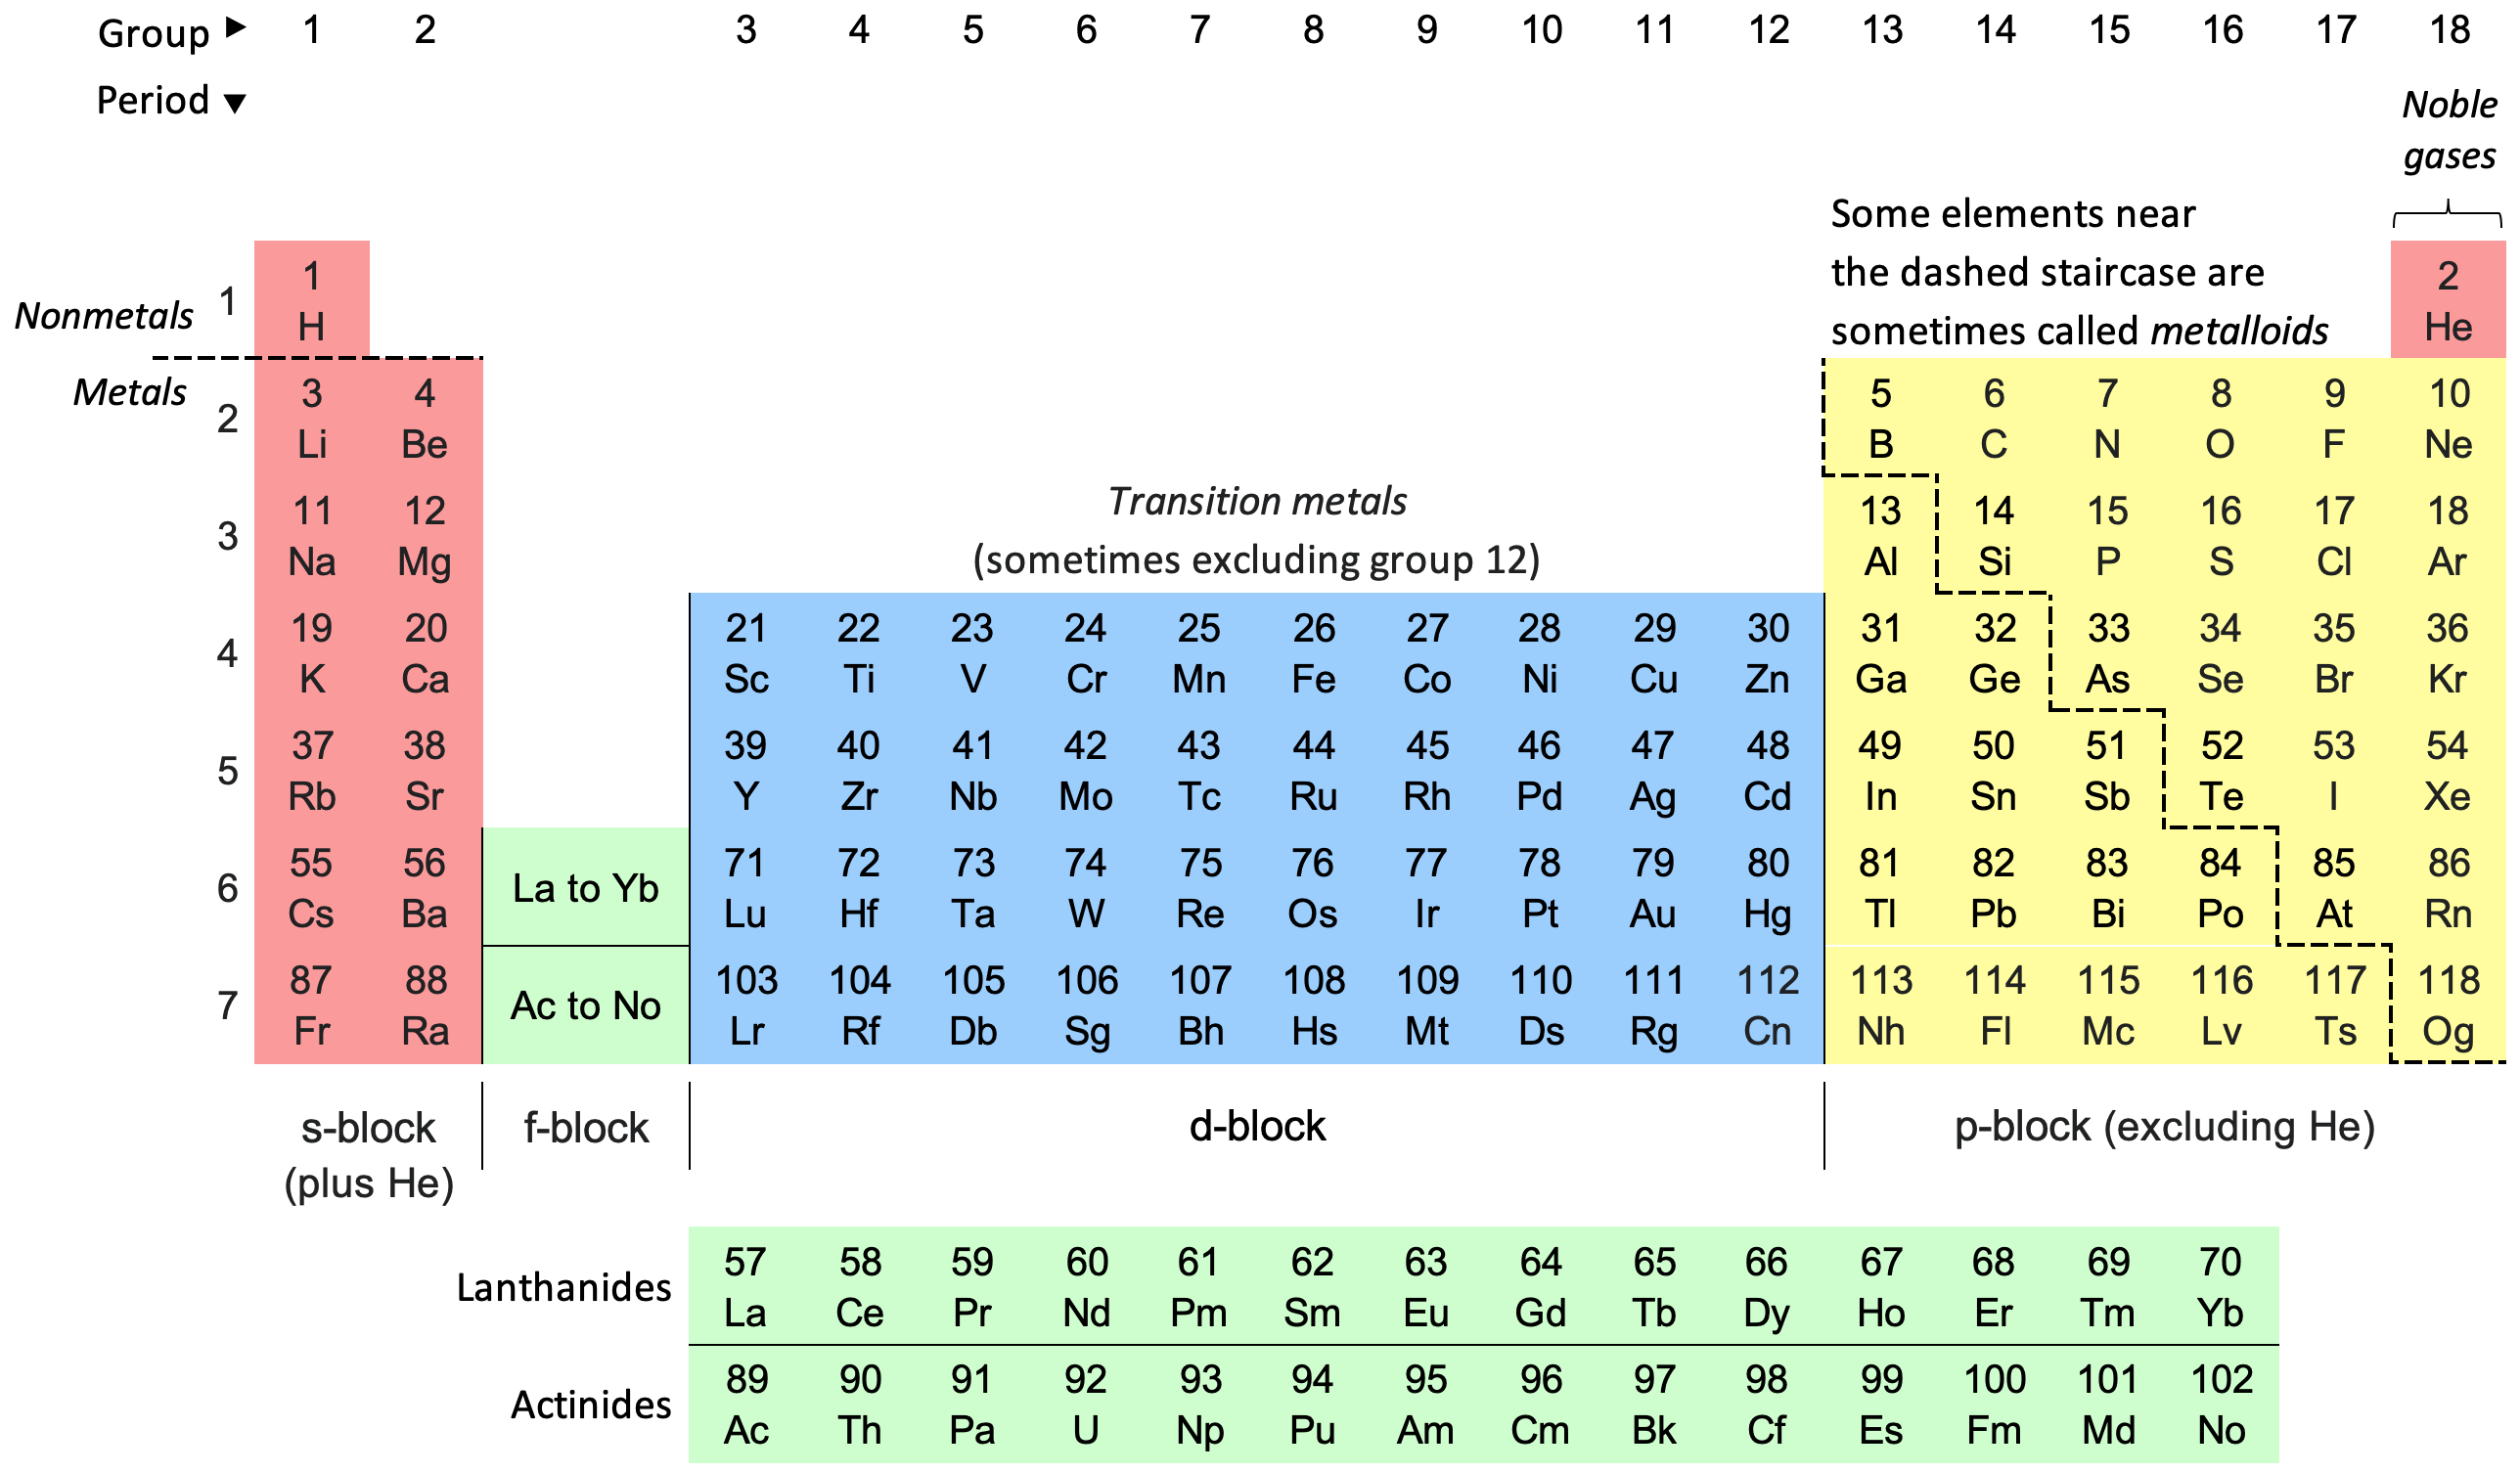
\includegraphics[width=0.9\textwidth]{periodic_table.png}
        \caption{The Periodic Table of the Elements. For formatting reasons, the lanthanides and actinides are traditionally shown below the rest of the table. Figure adapted from Wikipedia.}
    \end{figure}

    \subsection{Exchange and Parity in the Centre of Momentum Frame}
    Let's now consider the effects of exchanging two identical particles on their spatial wavefunction. Letting \(\vb{X}_1,\vb{P}_1\) and \(\vb{X}_2,\vb{P}_2\) denote position and momentum operators of the two particles, exchanging \(1\leftrightarrow 2\) implies that
    \begin{align}
        \vb{X}_{\text{com}}&=\frac{\vb{X}_1+\vb{X}_2}{2} & &\longmapsto & \frac{\vb{X}_2+\vb{X}_1}{2}&=\vb{X}_{\text{com}}\\
        \vb{P}_{\text{com}}&=\vb{P}_1+\vb{P}_2 & &\longmapsto & \vb{P}_2+\vb{P}_1&=\vb{P}_{\text{com}}\,,
    \end{align}
    whilst
    \begin{align}
        \vb{X}_{\text{rel}}&=\vb{X}_1-\vb{X}_2 & &\longmapsto & \vb{X}_2-\vb{X}_1&=-\vb{X}_{\text{rel}}\\
        \vb{P}_{\text{rel}}&=\frac{\vb{P}_1-\vb{P}_2}{2} & &\longmapsto & \frac{\vb{P}_2-\vb{P}_1}{2}&=-\vb{P}_{\text{rel}}\,.
    \end{align}
    Thus, exchange acts trivially on the centre-of-momentum coordinates, but acts on the relative coordinates just like a parity transformation. Since \(Y_\ell^m(-\vb{x})=(-1)^\ell Y_\ell^m(\vb{x})\) under parity, we see that if two identical particles have relative orbital angular momentum \(\ell\), the spatial part of the wavefunction will be either symmetric or antisymmetric under exchange according to whether \(\ell\) is odd or even.

    The behaviour of the entire state under exchange is determined by whether the particles in question are bosons or fermions. In the case of identical bosons, the spins must be combined to form a symmetric overall spin state when \(\ell\) is even, or an antisymmetric overall spin state when \(\ell\) is odd so as to ensure the overall state is always symmetric under exchange. For fermions, the opposite holds so as to ensure overall antisymmetry.
    
    If the neutrons are produced in a state where their relative orbital angular momentum is \(\ell\) in the centre of momentum frame, their spatial wavefunction acquires a factor of \((-1)^\ell\) under exchange of the two neutrons.

    \subsubsection{Identical Particles and Inelastic Collisions}\label{intrinsic_parity}
    The requirement that the state describing \(N\) identical bosons/fermions needs to be totally symmetric/antisymmetric under exchange of any pair of identical particles has important consequences in collision processes where such particles are created or destroyed.

    For example, consider an exotic type of `atom' consisting of a spin-0 pion (denoted by \(\pi^-\)) bound electromagnetically to a deuterium nucleus (denoted by \(D^+\) --- itself consisting of a proton and a neutron, bound together by the strong nuclear force). The bound state energy levels of this atom due to the electromagnetic Coulomb attraction between the \(\pi^-\) and \(D^+\) have the same form as in Hydrogen and, in particular, the ground state is \(\ket{1,0,0}\), an \(s\)-wave having \(\ell=0\). Because the pion is much heavier than the electron, the Bohr radius of the \(D^+\pi^-\) `atom' is much smaller than that of Hydrogen and the \(\pi^-\) wavefunction closely hugs the \(D^+\) nucleus. The \(D^+\) is known to have spin-1 whilst the \(\pi^-\) is spin zero, so the 1s ground state of the \(D^+\pi^-\) `atom' has total angular momentum \(j=1\).

    Now, as well as their electromagnetic interactions, the \(\pi^-\) and \(D^+\) also interact via the short-range strong nuclear force. This causes the `atom' to be unstable, with the \(\pi^-\) rapidly being absorbed by the \(D^+\), causing the system to disintegrate into a pair of neutrons (each denoted \(N\)):
    \begin{equation}
        \pi^- + D^+ \longrightarrow N+N\,.
    \end{equation}
    (In particle physics terminology, processes such as this, where different types of particles appear in the initial and final states, are known as \textit{inelastic}. An \textit{elastic} process is one in which the initial and final states contain the same particles.)

    Neutrons are fermions with spin-\(\frac{1}{2}\), so the final state must be antisymmetric under their exchange. One possibility is for their spins to combine into one of the triplets
    \begin{equation}
        \ket{\uparrow}\ket{\uparrow}\,,\quad\frac{1}{\sqrt{2}}\left(\ket{\uparrow}\ket{\downarrow}+\ket{\downarrow}\ket{\uparrow}\right)\,,\quad\ket{\downarrow}\ket{\downarrow}
    \end{equation}
    of symmetric spin-1 states, combined with a spatial wavefunction that is antisymmetric under exchange. From above, this will be the case if the relative orbital angular momentum of the two neutrons is odd. The other possibility is for the spins to form the antisymmetric spin-0 state
    \begin{equation}
        \frac{1}{\sqrt{2}}\left(\ket{\uparrow}\ket{\downarrow}-\ket{\downarrow}\ket{\uparrow}\right)
    \end{equation}
    combined with a relative spatial wavefunction of even \(\ell\).

    Total angular momentum is conserved, so the spin and orbital angular momentum of the final state must combine to give \(j=1\) as for the initial ground state of the \(\pi^- D^+\). A combined system with angular momenta \(\ell\) and \(s\) have total angular momentum \(j\in\{\ell+s,\ell+s-1,\dots,\abs{\ell-s}\}\) depending on the relative alignment of the two subsystems. Thus, in the case that the neutrons spins combine to the antisymmetric spin-0 state, \(j=\ell=1\). However, since this case requires \(\ell\) even for fermionic statistics, we see it is ruled out. The remaining case is that the neutrons combine to give the net spin-1, so that
    \begin{equation}
        j=1\in\{\ell+1,\ell,\ell-1\}\,.
    \end{equation}
    Since fermionic statistics here require that \(\ell\) is odd, the only possibility to get \(j=1\) is if \(\ell=1\) and the spin and orbital angular momenta of the neutron pair are neither perfectly aligned nor perfectly anti-aligned. Thus the final state has \(j=\ell=s=1\).

    These considerations also help us to determine the intrinsic parity of the pion. Recall that the parity operator \(\Pi\) acts on a state \(\ket{\vb{x}}\) as
    \begin{equation}
        \Pi\ket{\vb{x}}=\eta\ket{\vb{x}}\,,
    \end{equation}
    where the value of \(\eta\in\{+1,-1\}\) is known as the \textit{intrinsic parity} that, like spin, depends on the type of particle that the state \(\ket{\vb{x}}\) represents. More generally, if \(\ket{\vb{x}_1,\kappa_1;\vb{x}_2,\kappa_2;\dots;\vb{x}_N,\kappa_N}\) describe an \(N\)-particle state in which a particle of type \(\kappa_a\) is definitely located at \(\vb{x}_a\), then the parity operator acts as
    \begin{equation}
        \Pi\ket{\vb{x}_1,\kappa_1;\vb{x}_2,\kappa_2;\dots;\vb{x}_N,\kappa_N}=\eta_1\eta_2\dots\eta_N\ket{\vb{x}_1,\kappa_1;\vb{x}_2,\kappa_2;\dots;\vb{x}_N,\kappa_N}\,,
    \end{equation}
    where \(\eta_k=\pm 1\) is the intrinsic parity of the \(k^{\text{th}}\) particle that only depends on \(\kappa_k\). This holds whether or not the particles are distinguishable.

    Like the spin of fundamental particles, these intrinsic parities are independent of any details of the spatial wavefunction. Intrinsic parities thus have no effect in elastic processes, where the same particles are present in both the initial and final states. The intrinsic parity of a particle can often be determined by examining inelastic processes in which the particle
    participates.

    In the example \(\pi^- D^+\to N N\) above, equating the parities gives
    \begin{equation}
        \eta_\pi\eta_D=(-1)^\ell\eta_N^2=-1
    \end{equation}
    since the initial atomic state \(\ket{1,0,0}\) has \(\ell=0\) and hence no parity other than the intrinsic parities. Provided parity is conserved by the strong nuclear interactions causing this decay, we conclude that the \(\pi^-\) and \(D^+\) must have opposite intrinsic parity. Now, the \(D^+\) is predominantly an \(s\)-wave bound state of a proton and neutron, so \(\eta_D=(-1)^\ell\eta_P\eta_N=\eta_P\eta_N\), and furthermore the proton and neutron can always be chosen to have the same intrinsic parity since they are related by an `isospin' symmetry\footnote{The standard model has an (approximate) `internal' \(\SU(2)\) symmetry known as \textit{isospin} that rotates protons into neutrons; they are different states of the same \textit{nucleon}, somewhat like the two different spin states \(\ket{\uparrow},\ket{\downarrow}\) of the same electron}. Thus \(\eta_D=+1\) and hence the pion must have intrinsic parity \(\eta_\pi=-1\).

    As we mentioned in \cref{Chap:Parity}, one of the great surprises of particle physics came in the 1950's. Cosmic rays were found to contain various types of particles, including two of similar mass called the \(\tau^+\) and the \(\theta^+\). Both particles decay quickly, the predominant channels being
    \begin{equation}
        \theta^+\longrightarrow\pi^+ +\pi^0\qquad\text{and}\qquad\tau^+\longrightarrow\pi^+ +\pi^+ +\pi^-\,.
    \end{equation}
    The angular distribution of the pions in the final states could be observed in a cloud chamber or bubble chamber, and studying these patterns showed that the pions were produced in an \(\ell=0\) state in both cases. Since \(\eta_\pi=-1\) (irrespective of the electric charge of the pion, for the same isospin reason as above), the \(\theta^+\) should have intrinsic parity \(\eta_\theta=\eta_\pi^2=+1\), while the \(\tau^+\) should have \(\eta_\tau=-1\). However, as measurements improved the masses and lifetimes of the two particles became indistinguishable. The puzzle was resolved in 1956 when Lee and Yang proposed that the two particles were in fact one and the same, but that parity was not conserved in their decay process. Their proposal was largely ignored until Lee persuaded his colleague, Madame Chien-Shiung Wu, to test it using the decay of a certain isotope of cobalt. Wu's experiments showed that parity is indeed violated in the weak interactions. The fact that \(\vb{x}\to -\vb{x}\) is not a symmetry of Nature can be accommodated in QFT, though the deep reason for it remains mysterious\footnote{There are various natural ways for parity violation to originate in string theory, but needless to say none of them have been verified experimentally.}.

    \newpage
    \section{Perturbation Theory I: Time Independent Case}\label{Chap:Time_Independent_Perturbation}
    We've now come about as far as we can (in this course) relying purely on symmetry principles. The dynamics of systems of genuine physical interest is rarely simple enough to hope that we can solve it exactly, just using the general constraints of symmetry. In these circumstances we need to make some sort of approximation, treating our system as being `close to' some other system whose dynamics is sufficiently simple to be controllable. That is, we treat the difference between our actual system, whose experimental properties we care about, and our model system, whose description is simple enough that we can handle it, as a \textit{perturbation}. The whole art of a theoretical physicist lies in striking this balance; if one's model system is too simplistic, it might not provide a reasonable guide to the behaviour of the real case\footnote{A classic joke. Milk production at a dairy farm was low, so the farmer wrote to the local university, asking for help from academia. A multidisciplinary team of professors was assembled, headed by a theoretical physicist, and two weeks of intensive on-site investigation took place. The scholars then returned to the university, notebooks crammed with data, where the task of writing the report was left to the team leader. Shortly thereafter the physicist returned to the farm, saying to the farmer, ``I have the solution, but it works only in the case of spherical cows in a vacuum.''}, while if the model is overly complicated it may itself prove impossible to understand.

    There's nothing inherently quantum mechanical about the need to approximate a complicated system by a simpler one, but, fortunately, perturbation theory in quantum mechanics often turns out to be considerably easier than in classical dynamics, largely because of the vector space nature of \(\hb\). In this chapter and the next, we'll study various techniques to handle quantum mechanical perturbation theory, beginning with the simplest cases.

    \subsection{An Analytic Expansion}
    Let \(H\) be the Hamiltonian of the experimental system we wish to understand, and \(H_0\) be the Hamiltonian of our model system whose eigenstates and eigenvalues we already know. We hope that \(\Delta H=H-H_0\) is in some sense `small', so it may be treated as a perturbation. More specifically, we look for a parameter --- let's call it \(\lambda\) --- that our true Hamiltonian depends on such that at \(\lambda=0\), \(H=H_0\). For \(\lambda\in[0,1]\), define
    \begin{equation}
        H_\lambda=H_0+\lambda\Delta H\,.
    \end{equation}
    We can think of \(H_\lambda\) as the Hamiltonian of an apparatus that is equipped with a dial that allows us to vary \(\lambda\). At \(\lambda=0\) the system is our model case, and at \(\lambda=1\) it's the case of genuine interest.

    We now seek the eigenstates \(\ket{E_\lambda}\) of \(H_\lambda\). This may look as though we've made the problem even harder --- we now need to find the eigenstates not just of our model and experimental systems, but of a 1-parameter family of interpolating systems. Our key assumption is that since \(H_\lambda\) depends analytically on \(\lambda\), so too do its eigenstates. In essence, this amounts to the assumption that small changes in the system will lead to only small changes in the outcome. Every mountain climber knows that this assumption can be dreadfully false and we'll see that it can easily fail in QM too, but for now let's see where it takes us.

    If indeed \(\ket{E_\lambda}\) depends analytically in \(\lambda\), then we can expand it as
    \begin{equation}
        \ket{E_\lambda}=\ket{\alpha}+\lambda\ket{\beta}+\lambda^2\ket{\gamma}+\dots
    \end{equation}
    and similarly expand the eigenvalues
    \begin{equation}
        E(\lambda)=E^{(0)}+\lambda E^{(1)}+\lambda^2 E^{(2)}+\dots\,.
    \end{equation}
    Plugging these expansions into the defining equation \(H_\lambda\ket{E_\lambda}=E(\lambda)\ket{E_\lambda}\) we obtain
    \begin{equation}
        \begin{aligned}
            (H_0+\lambda\Delta H)&(\ket{\alpha}+\lambda\ket{\beta}+\lambda^2\ket{\gamma}+\dots)\\
            &=\left(E^{(0)}+\lambda E^{(1)}+\lambda^2 E^{(2)}+\dots\right)(\ket{\alpha}+\lambda\ket{\beta}+\lambda^2\ket{\gamma}+\dots)\,.
        \end{aligned}
    \end{equation}
    Since we require this to hold as \(\lambda\) varies, it must hold for each power of \(\lambda\) separately. Thus we find an infinite system of equations
    \begin{align}
        H_0\ket{\alpha}&=E^{(0)}\ket{\alpha}\,,\\
        H_0\ket{\beta}+\Delta H\ket{\alpha}&=E^{(0)}\ket{\beta}+E^{(1)}\ket{\alpha}\,,\label{first_order_perturbation}\\
        H_0\ket{\gamma}+\Delta H\ket{\beta}&=E^{(0)}\ket{\gamma}+E^{(1)}\ket{\beta}+E^{(2)}\ket{\alpha}\,,\label{second_order_perturbation}\\
        &\ \, \vdots\notag
    \end{align}

    The first of these equations simply states that \(\ket{\alpha}\) is an eigenstate of the model Hamiltonian \(H_0\) with eigenvalue \(E^{(0)}\). This is not surprising; under our analytic assumptions the terms of \(O(\lambda^0)\) are all that would survive when the dial is set to \(\lambda=0\), which is indeed the model system. Henceforth, we relabel \(\ket{\alpha}\to\ket{n}\) and \(E^{(0)}\to E_n\) to reflect this understanding. (The notation \(n\) is intended to imply the \(n^{\text{th}}\) energy eigenstate of the model Hamiltonian \(H_0\), with eigenvalue \(E_n\); we will distinguish the higher-order corrections to these states with superscripts.)

    To determine the first-order correction \(E_n^{(1)}\) to the \(n^{\text{th}}\) energy level of the unperturbed Hamiltonian, we contract the second equation (\ref{first_order_perturbation}) with \(\ket{\alpha}=\ket{n}\) to find
    \begin{equation}
        \mel{n}{H_0}{\beta}+\mel{n}{\Delta H}{n}=E_n\braket{n}{\beta}+E_n^{(1)}\,.
    \end{equation}
    Since the model Hamiltonian is Hermitian,
    \begin{equation}
        \mel{n}{H_0}{\beta}=\mel{\beta}{H_0}{n}^*=E_n\braket{n}{\beta}\,,
    \end{equation}
    so in the case that the unperturbed state is \(\ket{n}\), the equation becomes
    \begin{equation}\label{first_order_energy_perturbation}
        E_n^{(1)}=\expval{\Delta H}{n}\,.
    \end{equation}
    In other words, to first order in \(\lambda\), the change in the energy of our system as we move away from the model system is given by the expectation value \(\eval{\Delta H}_n\) of the change in the Hamiltonian when the system is in its original state \(\ket{n}\).

    To find the perturbed state to first order in \(\lambda\), we must understand \(\ket{\beta}\). We can expand \(\ket{\beta}\) in the complete set \(\ket{n}\) of eigenstates of the original system as
    \begin{equation}
        \ket{\beta}=\sum_n b_n\ket{n}\,.
    \end{equation}
    Using this expression in the second of equations (\ref{first_order_perturbation}) and contracting with \(\bra{m}\), where \(\bra{m}\ne\bra{n}\), the initial state we're perturbing, gives
    \begin{equation}
        (E_n-E_m)b_m=\mel{m}{\Delta H}{n}
    \end{equation}
    and so, provided \(E_m\ne E_n\),
    \begin{equation}\label{first_order_perturbation_coeff}
        b_m=\frac{\mel{m}{\Delta H}{n}}{E_n-E_m}\,.
    \end{equation}
    This will hold provided the energy levels of our model system are non-degenerate; we'll examine how to handle the more general case including degeneracy in \cref{Chap:Degenerate_PT}. In the non-degenerate case, equation (\ref{first_order_perturbation_coeff}) determines all the expansion coefficients \(b_m\) in \(\ket{\beta}\) except \(b_n\). Fortunately, one can argue that \(b_n=0\) from the requirement that \(\ket{E_\lambda}\) remains correctly normalised. This is left as an exercise, but the essential idea is that if we move a point on a unit sphere, then to first order \(\vb{r}\vdot\delta\vb{r}=0\) so that the variation is only nonzero in directions orthogonal to the original vector. With \(b_n=0\) we have
    \begin{equation}
        \ket{\beta}=\sum_{m\ne n}\frac{\mel{m}{\Delta H}{n}}{E_n - E_m}\ket{m}
    \end{equation}
    as the first-order perturbation of the state when the unperturbed state is \(\ket{n}\).

    We can also examine the second-order perturbation, \(E_n^{(2)}\), of the \(n^{\text{th}}\) energy level. To do so, contract the third of equations (\ref{second_order_perturbation}) with \(\bra{n}\). Using the facts that \(\mel{n}{H_0}{\gamma}=E_n\braket{n}{\gamma}\) and \(\braket{n}{\beta}=0\) we have
    \begin{align}
        E_n^{(2)}&=\mel{n}{\Delta H}{\beta}=\sum_{m\ne n}\frac{\mel{n}{\Delta H}{m}\mel{m}{\Delta H}{n}}{E_n - E_m}\notag\\
        &=\sum_{m\ne n}\frac{\abs{\mel{n}{\Delta H}{m}}^2}{E_n-E_m}\label{second_order_perturbation_energy}
    \end{align}
    using our expression for \(\ket{\beta}\). We could go on to higher order in \(\lambda\), next finding \(\ket{\gamma}\) in terms of the original states \(\{\ket{n}\}\) and then finding the third-order energy shift \(E_n^{(3)}\) \textit{etc.}, but in practice the summations become increasingly messy and we hope that the first few terms already provide a good guide to the behaviour of the system near \(\lambda=1\). (In high-energy quantum field theory, modern experiments typically cost many millions of dollars so it's especially important to have extremely accurate theoretical predictions to compare to. Consequently, there's a whole industry of people whose life's work is to compute higher and higher order terms in perturbation series such as these.) Fortunately, in the Tripos you'll never be asked to do anything beyond \(2^{\text{nd}}\) order.

    Combining our results shows that, to second order in \(\lambda\), the energy levels of the perturbed system are given by
    \begin{equation}
        E_n(\lambda)=E_n+\lambda\mel{n}{\Delta H}{n}+\lambda^2\sum_{m\ne n}\frac{\abs{\mel{n}{\Delta H}{m}}^2}{E_n - E_m}+O(\lambda^3)\,,
    \end{equation}
    where \(E_n\) are the energies of our model system. Recall that this expression --- much beloved of Tripos examiners --- is derived under the assumptions (i) that the new energies \(E(\lambda)\) and new states \(\ket{E_\lambda}\) are analytic at \(\lambda=0\) and (ii) that the model system is non-degenerate so \(E_m=E_n\) iff \(\ket{m}=\ket{n}\).
    
    Let's now take a look at the use of this formula in a number of examples.

    \subsubsection{Fine Structure of Hydrogen}\label{Chap:Hydrogen_Fine_Structure}
    Our treatment of the hydrogen atom in the last chapter assumed the electron was moving non relativistically in the Coulomb field of the proton. Since \(\abs{E/\mu c^2}=\alpha^2/2n^2\ll 1\), non-relativistic quantum mechanics should indeed be a good approximation. Nonetheless, better agreement with experiment is obtained by describing the electron using the relativistic Dirac equation\footnote{A better approximation still --- in precise agreement with the most accurate measurement ever performed in any branch of science --- comes from quantum field theory.}. The energy levels obtained by assuming non-relativistic motion in a pure Coulomb potential are often called the \textit{gross structure} of the hydrogen atom, whilst the small relativistic corrections to these energies implied by the Dirac equation are known as fine structure. We understood that gross structure energies are independent of \(\ell\) because of an enhanced symmetry of the pure Coulomb potential, generated by the Runge--Lenz operator. We thus expect that relativistic corrections will lift the degeneracy among states of different \(\ell\).

    The Dirac equation itself is beyond the scope of this course, but some of its consequences are easy to understand in perturbation theory. Firstly, expanding the relativistic dispersion relation around the non-relativistic limit gives
    \begin{equation}\label{relativistic_energy}
        E=\sqrt{\vb{p}^2c^2+\mu^2 c^4}\approx\mu c^2+\frac{\vb{p}^2}{2\mu}-\frac{\vb{p}^4}{8\mu^3 c^2}+\dots
    \end{equation}
    This shows that the relativistic correction to the kinetic energy is
    \begin{equation}\label{relativistic_KE_correction}
        \Delta H=-\frac{\vb{p}^4}{8\mu^3 c^2}
    \end{equation}
    at first order. From (\ref{first_order_energy_perturbation}), the first-order shift in the energy of state \(\ket{n,\ell,m}\) of hydrogen due to this modified kinetic term is thus
    \begin{equation}
        E_{n,\ell}^{(1)}=\expval{\Delta H}{n,\ell,m}\,.
    \end{equation}
    (In making this claim, we should note that our perturbation (\ref{relativistic_KE_correction}) is rotationally invariant, so in particular \([L_z,\Delta H]=0\) and \([\vb{L}^2,\Delta H]=0\). Therefore \(\mel{n,\ell',m'}{\Delta H}{n,\ell,m}=0\) unless \(\ell'=\ell\) and \(m'=m\). Thus our perturbation does not mix degenerate states of the gross structure, so non-degenerate perturbation theory is sufficient.)

    To compute the first order energy correction, first we note that
    \begin{equation}
        \Delta H=-\frac{(H_0-V(r))^2}{2\mu c^2}\,,
    \end{equation}
    where \(H_0\) is the gross structure Hamiltonian and \(V(r)\) is the usual Coulombic potential. Then
    \begin{equation}
        E_{n,\ell}^{(1)}=-\frac{1}{2\mu c^2}[(E_n)^2-2E_n\eval{V(r)}+\eval{V(r)^2}]\,,
    \end{equation}
    where \(E_n=-\frac{1}{2}\mu c^2\alpha^2/n^2\) is the energy of the unperturbed state and \(\eval{V(r)}=\expval{V(r)}{n,\ell,m}\). The virial theorem for the \(1/r\) potential tells us that \(2\eval{T}=-\eval{V}\), so \(\eval{V}=2E_n\). Next, to compute \(\eval{V^2}\), observe that this \(1/r^2\) term just modifies the effective potential due to the electron's orbital angular momentum. Consider the Hamiltonian for the radial part of the Hydrogen atom, but now with an effective potential
    \begin{equation}
        V_{\text{eff}}(r)=\frac{\hbar^2}{2\mu}\frac{\ell(\ell+1)}{r^2}+\frac{\alpha}{r}-\frac{e^2}{4\pi\epsilon_0 r}=\frac{\hbar^2}{2\mu}\frac{\ell'(\ell'+1)}{r^2}-\frac{e^2}{4\pi\epsilon_0 r}\,.
    \end{equation}
    Here we've introduced \(\ell'\) to absorb the extra \(\alpha/r^2\) term into the angular momentum contribution. Of course \(\ell'\) does not correspond to any actual angular momentum. It's just a trick to help us compute \(\eval{V^2}\). With this effective potential, repeating the calculations of \cref{Chap:Coulomb_Radial_Hamiltonian} would lead to just the same energy levels as before, but now in terms of (non-integer) \(\ell'\) instead of \(\ell\):
    \begin{equation}
        E(\ell')=-\frac{1}{2}\mu c^2\alpha^2\frac{1}{(\ell'+1)^2}\,.
    \end{equation}
    This is the exact result for a hydrogen atom with an additional \(1/r^2\) term in its potential. However, in our perturbative context, it's only appropriate to keep the answer accurate to first order --- there may be other effects we haven't yet accounted for (such as expanding (\ref{relativistic_energy}) further) that contribute at higher order. Expanding \(\ell'\) around \(\ell\) we find
    \begin{equation}
        E(\ell')=E_n+\frac{1}{2}\mu c^2\frac{\alpha^4}{n^3(\ell+\frac{1}{2})}+\dots
    \end{equation}
    where \(n=\ell+1\). Combining this with the other terms gives
    \begin{equation}\label{relativistic_correction}
        E_{n,\ell}^{(1)}=-\frac{1}{2}\mu c^2\left(\frac{n}{\ell+\frac{1}{2}}-\frac{3}{4}\right)\frac{\alpha^4}{n^4}
    \end{equation}
    as the first-order change in the energy of state \(\ket{n,\ell,m}\) due to the relativistic correction to kinetic energy. Notice that this effect is suppressed by an additional power of \(\alpha^2\sim v^2/c^2\) compared to the gross structure, and that the degeneracy among states of different \(\ell\) is lifted, as we expected.

    There's a second consequence of the Dirac's equation which comes in at the same order as the above kinetic terms. Due to its spin, the electron has a magnetic dipole moment
    \begin{equation}
        \vb{m}=-\frac{e}{2\mu}\vb{S}\,.
    \end{equation}
    When placed in a magnetic field, the dipole has energy \(U=-\vb{m}\vdot\vb{B}\). Relativistically, the electron in a Hydrogen atom does experience a magnetic field because it moves through the electric field \(\vb{E}\) produced by the proton. If the electron has velocity \(\vb{v}=\vb{p}/\mu\gamma\), then classically the Lorentz transformation of \(\vb{E}\) produces a magnetic field
    \begin{equation}
        \vb{B}=\frac{\gamma}{c^2}\vb{v}\cross\vb{E}=\frac{1}{\mu c^2}\vb{p}\cross\left(\frac{e\vu{r}}{4\pi\epsilon_0 r^2}\right)=-\frac{e}{4\pi\epsilon_0\mu c^2}\frac{1}{r^3}\vb{L}\,.
    \end{equation}

    Consequently, in QM the Hamiltonian of hydrogen receives a further fine-structure correction
    \begin{equation}
        H_{\text{SO}}=-\vb{m}\vdot\vb{B}=\frac{\alpha\hbar^3}{2\mu^2 c}\frac{1}{r^3}\vb{S}\vdot\vb{L}
    \end{equation}
    known as the \textit{spin-orbit coupling}. Since the coefficient of the operator \(\vb{S}\vdot\vb{L}\) is positive, spin-orbit coupling lowers the total energy when the spin and orbital angular momentum are antiparallel. In particular, \(\vb{S}\vdot\vb{L}\) vanishes in any state of hydrogen in which \(\ell=0\), since then all components of \(\vb{L}\) act trivially. As an important special case, spin-orbit coupling does not affect the ground state. However, excited states with \(\ell\ne 0\) do generically feel the effects of spin-orbit coupling.

    We first compute the effect of acting on our electron states with \(\vb{L}\vdot\vb{S}\). To do this, clearly we must include a specification of the electron's spin. This could be done using the basis
    \begin{equation}
        \{\ket{n,\ell,m}\otimes\ket{\uparrow},\ket{n,\ell,m}\otimes\ket{\downarrow}\}\,,
    \end{equation}
    but it turns out to be more convenient to instead combine the electron's orbital and spin angular momenta to \(\vb{J}=\vb{L}+\vb{S}\) and label states by\footnote{Since \([\vb{J},\vb{L}^2]=0\), it's possible to find a basis of simultaneous eigenstates of \(\vb{J}^2\), \(\vb{J}_z\) and \(\vb{L}^2\). In this basis, we do not necessarily know the \(z\)-components of the electron's orbital and spin angular momenta separately.} \(\ket{n,j,m_j;\ell}\) where \(j=\ell+\frac{1}{2}\) or \(j=\ell-\frac{1}{2}\) are the two possible values for the combined angular momentum, and \(\abs{m_j}\le j\). To make use of this, we write
    \begin{equation}
        \vb{S}\vdot\vb{L}=\frac{1}{2}(\vb{J}^2-\vb{L}^2-\vb{S}^2)\,.
    \end{equation}
    Thus
    \begin{align}
        \vb{S}\vdot\vb{L}\ket{n,j,m_j;\ell}&=\frac{\hbar^2}{2}\left(j(j+1)-\ell(\ell+1)-\frac{3}{4}\right)\ket{n,j,m_j,\ell}\\
        &=\frac{\hbar^2}{2}\begin{cases}
            \ell\ket{n,j,m_j;\ell} & \text{when }j=\ell+\frac{1}{2}\\
            -(\ell+1)\ket{n,j,m_j;\ell} & \text{when }j=\ell-\frac{1}{2}\,.
        \end{cases}
    \end{align}
    Consequently, the first order change in the energy of the \(\ket{n,j,m_j;\ell}\) state of hydrogen due to spin-orbit coupling is
    \begin{equation}
        E_{n,j;\ell}^{(1)}=-\frac{1}{4\mu^2 c^2}\frac{e^2\hbar^2}{4\pi\epsilon_0}\left\{\begin{matrix}
            \ell \\ -(\ell+1)
        \end{matrix}\right\}\eval{\frac{1}{r^3}}_{n,j;\ell}\,,
    \end{equation}
    where the factor of \(\ell\) or \(-(\ell+1)\) chosen depending on whether \(j=\ell\pm\frac{1}{2}\).

    To compute the expectation value \(\eval{1/r^3}_{n,j;\ell}\) we could just perform the integral
    \begin{equation}
        \int_{\RR^3}\dd[3]{\vb{x}}\abs{\psi_{n,l,m}(\vb{x})}^2\frac{1}{r^3}\,.
    \end{equation}
    However, there is a trick that allows us to short-circuit the evaluation of this integral. Recall that for states of definite \(\ell\), the Hamiltonian for the unperturbed atom can be written
    \begin{equation}
        H_{\ell}=-\frac{P_r^2}{2\mu}+\frac{\hbar^2\ell(\ell+1)}{2\mu r^2}-\frac{e^2}{4\pi\epsilon_0 r}\,,
    \end{equation}
    where \(P_r=(\vu{X}\vdot\vb{P}+\vb{P}\vdot\vu{X})/2\) is the radial momentum given by
    \begin{equation}
        P_r=-\ii\hbar\left(\pdv{}{r}+\frac{1}{r}\right)
    \end{equation}
    in the position representation. Now, the expectation value \(\eval{[P_r,H_\ell]}=0\) when evaluated in any normalisable eigenstate of \(H_\ell\). In our case, the commutator evaluates to
    \begin{equation}
        [P_r,H_\ell]=-\ii\hbar\left(-\frac{\hbar^2\ell(\ell+1)}{\mu r^3}+\frac{e^2}{4\pi\epsilon_0 r^2}\right)
    \end{equation}
    and therefore, provided \(\ell\ne 0\),
    \begin{equation}
        \eval{\frac{1}{r^3}}_{n,j;\ell}=\frac{1}{a_0}\frac{1}{\ell(\ell+1)}\eval{\frac{1}{r^2}}_{n,j;\ell}=\frac{1}{a_0^3}\frac{1}{\ell(\ell+\frac{1}{2})(\ell+1)}\frac{1}{n^3}\,,
    \end{equation}
    where \(a_0=\hbar/\alpha\mu c\) is the Bohr radius and the second equality follows from our previous result for \(\eval{1/r^2}\).

    Putting all these together, the first-order energy shifts due to spin-orbit coupling are
    \begin{equation}\label{spin_orbit_aligned}
        E_{n,j;\ell}^{(1)}=+\frac{1}{2}\alpha^4\mu c^2\frac{1}{2n^3(\ell+\frac{1}{2})(\ell+1)}
    \end{equation}
    when \(j=\ell+\frac{1}{2}\), whereas when \(j=\ell-\frac{1}{2}\) we have
    \begin{equation}\label{spin_orbit_antialigned}
        E_{n,j;\ell}^{(1)}=-\frac{1}{2}\alpha^4\mu c^2\frac{1}{2n^3\ell(\ell+\frac{1}{2})}\,.
    \end{equation}
    (Also recall that \(E_{n,j;\ell}^{(1)}=0\) if \(\ell=0\).) As anticipated, states whose spin and orbital angular momenta are anti-aligned (\(j=\ell-\frac{1}{2}\)) have lower energy and so are more tightly bound than the pure Coulomb interaction, whereas if the spin and orbital angular momentum are aligned with each other (\(j=\ell+\frac{1}{2}\)) the state is less tightly bound. Notice also that the deviation from a pure Coulombic interaction partially lifts the degeneracy between states of different \(\ell\).

    We can also see that the spin-orbit contribution to the energy is suppressed by a factor of \(\alpha^2\) compared to the gross structure energy \(-\frac{1}{2}\mu\alpha^2c^2/n^2\). This is the same suppression as we found for the \(\vb{P}^4\) correction to the kinetic term, so it does not really make sense to consider these two effects on the energy separately. Combining (\ref{relativistic_correction}) with (\ref{spin_orbit_aligned}) and (\ref{spin_orbit_antialigned}), we find the net energy levels
    \begin{equation}\label{fine_structure}
        E_{n,j;\ell}=-\frac{1}{2}\mu\alpha^2 c^2\left[\frac{1}{n^2}-\frac{\alpha^2}{n^3}\left(\frac{3}{4n}-\frac{1}{j+\frac{1}{2}}\right)+\dots\right]
    \end{equation}
    incorporating fine structure correct to order \(\alpha^4\). This formula holds regardless of whether \(j=\ell+\frac{1}{2}\) or \(j=\ell-\frac{1}{2}\). Even better, although the spin-orbit term contributes only when \(\ell\ne 0\), it turns out that there is another term\footnote{This remaining relativistic effect is known as the Darwin term and gives a contribution \(\frac{\alpha\pi\hbar^3}{2\mu^2 c}\delta(\vb{x})\). The origin of this term is rather subtle, and properly lies within QFT rather than QM. Because of the \(\delta\)-function, it only affects states which have non-zero probability to be found at \(r=0\). The only such states are those with \(\ell=0\), since all others are prevented from reaching the origin by the effective potential \(\ell(\ell+1)/2mr^2\).} that contributes only when \(\ell\) does equal zero! Even better, this remaining term has the effect that (\ref{fine_structure}) is the correct fine structure energy levels even for states with \(\ell=0\) where \(j=\frac{1}{2}\) just from the spin.

    Proceeding down the periodic table, if we attach a single electron to an atomic nucleus containing \(Z\) protons, the bare Coulomb interaction increases by a factor of \(Z\). The formula (\ref{fine_structure}) remains valid provided we replace \(\alpha\sim e^2\) by \(Z\alpha\). Hydrogen has \(Z=1\), so in the \(n=1\) ground state the fine structure contribution is suppressed by a factor of \(\alpha^2\sim 1/(137)^2\) compared to the gross structure, justifying our treatment of the fine structure as a small perturbation. However, for heavier elements with higher \(Z\), the suppression is only by \((Z\alpha)^2\) and the small value of \(\alpha\) can be negated by a sufficiently large \(Z\). In particular, from (\ref{fine_structure}) we see that the energy difference between the states with principal quantum number \(n\) but \(j=\ell\pm\frac{1}{2}\) is
    \begin{equation}
        E_{n,\ell+\frac{1}{2};\ell}-E_{n,\ell-\frac{1}{2};\ell}=\frac{1}{2}\mu c^2\frac{1}{n^3}\frac{Z^4\alpha^4}{\ell(\ell+1)}\,.
    \end{equation}
    This gives the splitting between the two 2p states of Hydrogen to be \(4.53\times 10^{-5}\unit{eV}\), in excellent agreement with the measured value of \(4.54\times 10^{-5}\unit{eV}\). These splittings reach around 10\% of the gross energy as one reaches the middle of the periodic table, making perturbative treatments less reliable.

    \subsubsection{Hyperfine Structure of Hydrogen}
    A proton is a spin-\(\frac{1}{2}\) particle, so like the electron it has a magnetic dipole moment \(\vb{m}_p\) proportional to its spin. A magnetic dipole \(\vb{m}_p\) placed at the origin generates its own magnetic field
    \begin{equation}
        \vb{B}=\frac{2\mu_0}{3}\vb{m}_p\delta(\vb{x})+\frac{\mu_0}{4\pi r^3}(3(\vb{m}_p\vdot\vu{r})\vu{r}-\vb{m}_p)\,,
    \end{equation}
    which is roughly the field you saw traced out by iron lings when first playing with magnets. The dipole moment \(\vb{m}_e\) of the electron sits inside this field, leading to a new contribution
    \begin{equation}
        H_{\text{hfs}}=-\vb{m}_e\vdot\vb{B}
    \end{equation}
    depending on both dipoles. We'll just investigate the effect of this perturbation on the \(\ell=0\) state of hydrogen, where it turns out that only the first term \(\sim\delta(\vb{x})\) in \(\vb{B}\) has non-vanishing contribution. For these \(\ell=0\) states, one finds
    \begin{equation}\label{hyper_fine_hamiltonian}
        H_{\text{hfs}}=\frac{4}{3}\frac{m}{M}\alpha^4\mu c^2\frac{1}{n^3\hbar^2}\vb{S}\vdot\vb{I}\,,
    \end{equation}
    where \(\vb{I}\) is the spin operator for the proton, labelled using a different letter to avoid confusion with the electron spin operator \(\vb{S}\).

    The splittings in energy levels caused by this perturbation are suppressed not just by a factor of \(\alpha^4\), but by an additional factor of the electron-to-proton mass ratio \(m/M\approx 1/1836\). The splittings caused by accounting for nuclear spin are thus much smaller than those of the fine structure considered above, and the perturbation (\ref{hyper_fine_hamiltonian}) is known as the \textit{hyperfine} contribution to the energy levels. We can compute the eigenvalues in much the same way as for the spin-orbit contribution to fine structure. Let \(\vb{F}=\vb{I}+\vb{S}\) denote the total spin of the proton and electron. Then
    \begin{equation}
        (\vb{S}\vdot\vb{I})=\frac{1}{2}(\vb{F}^2-\vb{I}^2-\vb{S}^2)=\frac{\hbar^2}{2}\left(f(f+1)-\frac{3}{2}\right)\,.
    \end{equation}
    This is \(-3\hbar^2/4\) when the proton and electron spins are antiparallel so \(f=0\), and \(+\hbar^2/4\) when \(f=1\). Plugging these into (\ref{hyper_fine_hamiltonian}) shows that the difference between the energies for the \(n=1\) ground state of hydrogen is
    \begin{equation}
        E_{n=1;f=+1}-E_{n=1;f=0}=\frac{4}{3}\frac{m}{M}\alpha^4\mu c^2\approx 5.88\times 10^{-6}\unit{eV}\,,
    \end{equation}
    corresponding to a frequency of \(1.4\unit{GHz}\) and a wavelength of \(21\unit{cm}\). Thus transitions between the energy levels split by the hyperfine structure causes the hydrogen atom to have a microwave emission line.

    The \(21\unit{cm}\) line provides the most powerful way of tracing diffuse gas in interstellar and intergalactic space. This wavelength is much longer than the size of typical specks of dust, so \(21\unit{cm}\) radiation can propagate with little absorption right through clouds of dust and gas that do absorb visible light. It was radiation at \(1.4\unit{GHz}\) that first revealed the large scale structure of our galaxy. The line is intrinsically very narrow, so the temperature and radial (with the Earth as origin) velocity of the hydrogen that emitted the radiation can be accurately measured from the Doppler shift and broadening of the observed spectral line.

    The hyperfine structure of hydrogen leading to this \(21\unit{cm}\) emission line was first predicted theoretically in 1944 by the Dutch physicist H.C. van de Hulst as part of his doctoral thesis, carried out in Utrecht which was then under Nazi occupation. \(21\unit{cm}\) radiation from our galaxy was first detected experimentally in 1951 by three groups working independently in the USA, Australia and the Netherlands. The Dutch group used a German radio antenna left over from the war.

    \subsubsection{The Ground State of Helium}
    After hydrogen, helium is the next most abundant element, making up about a quarter of the ordinary matter in the Universe. Much of this helium was created during the period of nucleosynthesis, a tiny fraction of a second after the Big Bang.

    Let's use perturbation theory to find an estimate of the ground state energy of helium. Working in the centre of mass frame and treating the nucleus as stationary at the origin, the (gross structure) Hamiltonian is
    \begin{equation}
        H=\frac{\vb{P}_1^2}{2m}+\frac{\vb{P}_2^2}{2m}-\frac{2e^2}{4\pi\epsilon_0\abs{\vb{X}_1}}-\frac{2e^2}{4\pi\epsilon_0\abs{\vb{X}_2}}+\frac{e^2}{4\pi\epsilon_0}\frac{1}{\abs{\vb{X}_1-\vb{X}_2}}\,,
    \end{equation}
    where \((\vb{X}_1,\vb{X}_2)\) are the position operators and \((\vb{P}_1,\vb{P}_2)\) are the momentum operators for the two electrons. The terms describing the electrons' kinetic energy and attraction to the nucleus are just the sum of those for hydrogen, expect with \(e^2\) replaced by \(2e^2\) since there are two protons in the nucleus of helium. We'll take these terms to be the model Hamiltonian \(H_0\), treating the remaining electron-electron repulsion as a perturbation.

    In the unperturbed Hamiltonian, single-electron states are just the usual hydrogenic states \(\ket{n,\ell,m}\) with energy
    \begin{equation}
        -4\times\frac{1}{2}mv^2\alpha^2\frac{1}{n^2}\,,
    \end{equation}
    where the factor of 4 arise because each electron's attraction to the helium nucleus is twice as strong as it was for hydrogen. Since electrons are fermions, the total state of the neutral helium atom must be antisymmetric under their exchange. In particular, the ground state is
    \begin{equation}
        \ket{\Psi_0}=\ket{1,0,0}\otimes\ket{1,0,0}\otimes\frac{1}{\sqrt{2}}\left(\ket{\uparrow}\ket{\downarrow}-\ket{\downarrow}\ket{\uparrow}\right)
    \end{equation}
    where the final factor is the antisymmetric spin state of the two spin-\(\frac{1}{2}\) electrons.  (Note that,at the level of the gross structure of helium, the Hamiltonian is independent of the spins of the two electrons, so we are free to seek simultaneous energy and spin eigenstates.) This state is an eigenstate of the model Hamiltonian \(H_0\) with energy
    \begin{equation}
        E_1=-\frac{4\alpha^2}{2}mc^2-\frac{4\alpha^2}{2}mc^2=-2\alpha^2 mc^2\approx -108.8\unit{eV}\,,
    \end{equation}
    being the sum of the energies of the two electrons individually.

    We now take account of the electron-electron repulsion. To use perturbation theory, we set
    \begin{equation}
        \Delta H=\frac{e^2}{4\pi\epsilon_0}\frac{1}{\abs{\vb{X}_1-\vb{X}_2}}=\frac{\alpha\hbar c}{\abs{\vb{X}_1-\vb{X}_2}}\,.
    \end{equation}
    The first order shift in the ground state energy is
    \begin{align}
        \mel{\Psi_0}{\Delta H}{\Psi_0}&=\int\dd[3]{\vb{x}_1'}\dd[3]{\vb{x}_2'}\dd[3]{\vb{x}_1}\dd[3]{\vb{x}_2}\braket{\Psi_0}{\vb{x}_1'\vb{x}_2'}\mel{\vb{x}_1'\vb{x}_2'}{\Delta H(\vb{X}_1,\vb{X}_2)}{\vb{x}_1\vb{x}_2}\braket{\vb{x}_1\vb{x}_2}{\Psi_0}\notag\\
        &=\int\dd[3]{\vb{x}_1}\dd[3]{\vb{x}_2}\Psi_0(\vb{x}_1,\vb{x}_2)^*\frac{\alpha\hbar c}{\abs{\vb{x}_1-\vb{x}_2}}\Psi_0(\vb{x}_1,\vb{x}_2)\notag\\
        &=\int\dd[3]{\vb{x}_1}\dd[3]{\vb{x}_2}\frac{\alpha\hbar c}{\abs{\vb{x}_1-\vb{x}_2}}\abs{\psi_{100}(\vb{x}_1)}^2\abs{\psi_{100}(\vb{x}_2)}^2\,.
    \end{align}
    Here \(\psi_{100}(\vb{x})\) are the single-electron \(n=1\) wavefunctions
    \begin{equation}
        \psi_{100}=\frac{1}{\sqrt{\pi}}\left(\frac{2}{a_2}\right)^{\frac{3}{2}}\ee^{-\abs{\vb{x}}/a_2}\,,
    \end{equation}
    where the length scale \(a_2=\frac{\hbar}{2\alpha mc}\) is half the Bohr radius in hydrogen. In going to the last line, we've used the fact that the interaction is independent of spin, and the spin states have unit norm.

    Performing the integral is straightforward but somewhat tedious\footnote{In case you are curious: Choose the \(z\)-axis of \(\vb{x}_2\) to be aligned with whatever direction \(\vb{r}_1\). Then \(\abs{\vb{x}_1-\vb{x}_2}=\sqrt{\abs{r_1^2+r_2^2-2r_1r_2\cos\theta_2}}\), independent of \(\phi_2\). So
    \begin{equation}
        \eval{\Delta H}{\Psi_0}=\frac{4\alpha\hbar c}{a_2^3}\int\dd[3]{\vb{x}_1}\abs{\psi_{100}(\vb{x}_1)}^2\left[\int\dd{r_2}\dd{\theta_2}\frac{r_2^2\sin\theta_2 \ee^{-r_2/a_2}}{\sqrt{\abs{r_1^2+r_2^2-2r_1r_2\cos\theta_2}}}\right]\,.
    \end{equation}
    The integral in square brackets can be done using
    \begin{equation}
        \int_0^\pi\dd{\theta_2}\frac{\sin\theta_2}{\sqrt{\abs{r_1^2+r_2^2-2r_1r_2\cos\theta_2}}}=\frac{1}{r_1r_2}\int_0^\pi\dd{\theta_2}\dv{}{\theta_2}\sqrt{\abs{r_1^2+r_2^2-2r_1r_2\cos\theta_2}}=\begin{cases}
            2/r_1 & \text{when }r_1>r_2\\
            2/r_2 & \text{when }r_1<r_2\,.
        \end{cases}
    \end{equation}
    Thus the radial integral \(\dd{r_2}\) must be broken into two regions. Letting \(\rho_1=2r_1/a_2\) be a rescaled radial coordinate, we have
    \begin{align}
        \eval{\Delta H}{\Psi_0}&=\frac{8\alpha\hbar c}{a_2^3}\int\dd[3]{\vb{x}_1}\abs{\psi_{100}(\vb{x}_1)}^2\left[\int_0^{r_1}\dd{r_2}\frac{r_2^2}{r_1}\ee^{-2r_2/a_2}+\int_{r_1}^{\infty}\dd{r_2} r_2 \ee^{-2r_2/a_2}\right]\notag\\
        &=\frac{4\alpha\hbar c}{a_2}\int\dd[3]{\vb{x}_1}\abs{\psi_{100}(\vb{x}_1)}^2\frac{2-\ee^{-\rho_1}(2+\rho_1)}{\rho_1}\notag\\
        &=\frac{2\alpha\hbar c}{a_2}\int_{0}^{\infty}\dd{\rho_1}\rho_1 \ee^{-\rho_1}(2-\ee^{-\rho_1}(2+\rho_1))=\frac{5\alpha\hbar c}{4a_2}\,.
    \end{align}}. We have
    \begin{equation}
        \eval{\Delta H}{\Psi_0}=\frac{5}{4}\alpha^2 mc^2\,.
    \end{equation}
    As we suspected, this perturbation is also of order \(\alpha^2\) just like the leading-order term. Hence we get the ground state energy of Helium corrected to first order as
    \begin{equation}
        E=-4\alpha^2mc^2\left(1-\frac{5}{16}\lambda\right)_{\lambda=1}\approx -74.6\unit{eV}\,.
    \end{equation}
    This is in significantly better agreement with the experimental value of \(\approx-79.0\unit{eV}\) than the zeroth order estimate. Including the second-order term leads to
    \begin{equation}
        E=-4\alpha^2mc^2\left(1-\frac{5}{16}\lambda+\frac{25}{1024}\lambda^2\right)_{\lambda=1}\approx -77.5\unit{eV}\,.
    \end{equation}
    Given the crudity of our expansion this is remarkably close agreement with the experimental value.

    In heavy atoms, the ground state energy itself is difficult to measure experimentally since it involves computing the energy required to strip off all the electrons from the nucleus. Fortunately, for the same reason it's also rarely the directly relevant quantity. Instead, chemists and spectroscopists are usually more interested in the first ionisation energy, defined to be the energy required to liberate a single electron from the atom. Hydrogen only has one electron, so its first ionization energy is just the \(13.6\unit{eV}\) which we must supply to eject this electron from the ground state of the atom. In the case of helium, once one electron is stripped away the remaining electron sees the full force of the Coulomb potential from the \(Z=2\) nucleus, so will have binding energy \(-54.4\unit{eV}\). The first ionisation energy is thus the difference (\(-54.4+79.0)\unit{eV}=24.6\unit{eV}\). This is significantly greater than the ionisation energy of hydrogen, and in fact helium has the greatest first ionisation energy of any of the elements, reflecting its status as the first noble gas.

    \begin{figure}
        \centering
        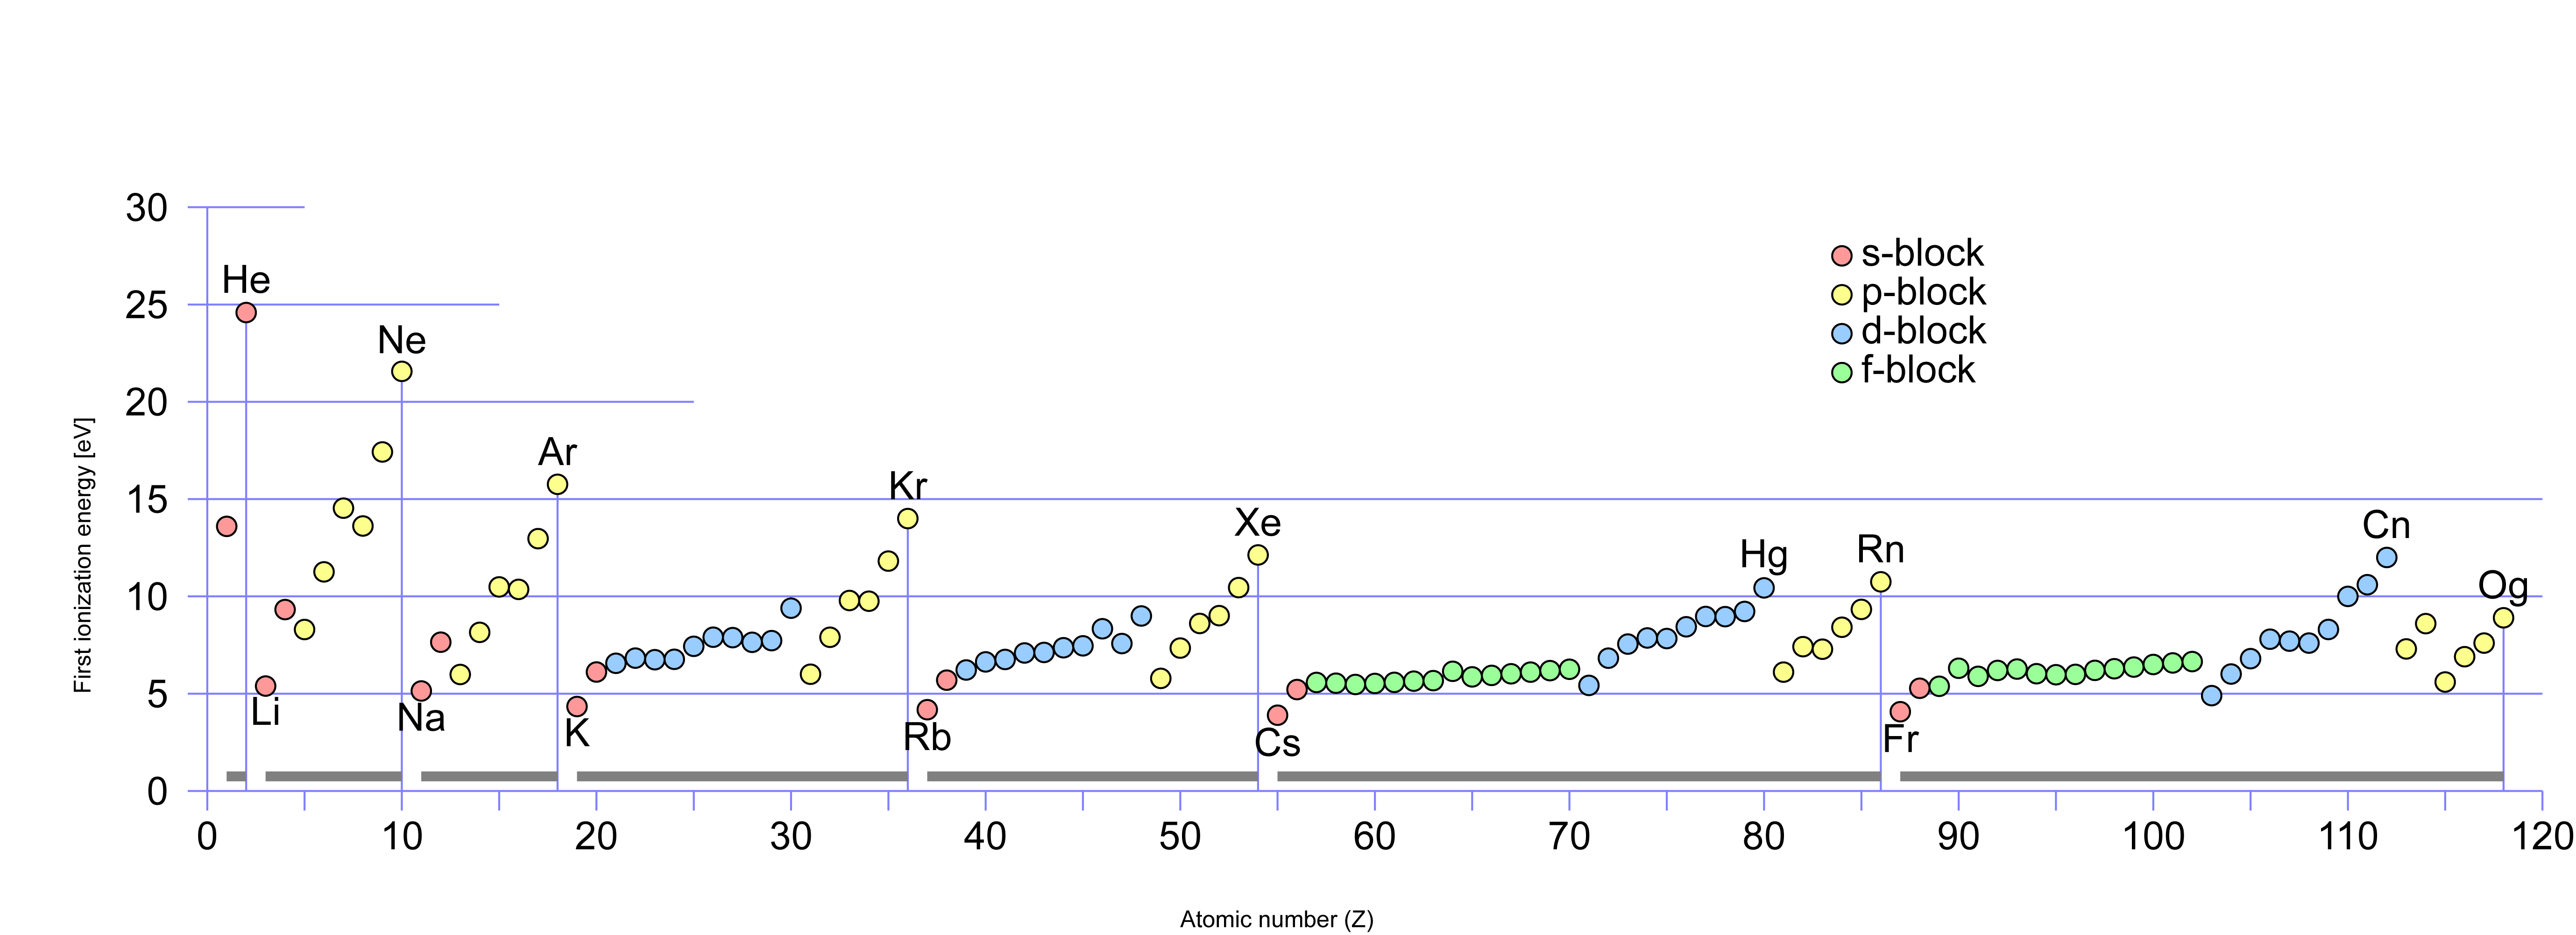
\includegraphics[width=\textwidth]{IE.png}
        \caption{First ionisation energies of the ground states of the first few elements. Figure adapted from Wikipedia.}
    \end{figure}

    \subsubsection{The Quadratic Stark Effect}
    We'll now consider a different type of perturbation, caused not by relativistic corrections to the Hamiltonian of the isolated atom, but by allowing the atom to interact with some external system.

    Suppose a hydrogen atom is placed in an external electric field \(\vb{E}=-\grad\phi\). Most electric fields we can generate in the laboratory are small compared to the strength of the Coulomb field felt by the electron due to the nucleus\footnote{With modern high intensity lasers, electric fields comparable to the nuclear Coulomb potential can be generated. The behaviour of a hydrogen atom in such a laser must be studied by other methods.}, so perturbation theory should provide a good estimate of the energy shifts such an external field induces. By definition of the electrostatic potential \(\phi\), the field changes the energy of the atom by \(E=e(\phi(\vb{x}_p)-\phi(\vb{x}_e))\) where \(\vb{x}_p\) and \(\vb{x}_e\) are the locations of the proton and electron. We assume the external field varies only slowly over scales of order the Bohr radius, so
    \begin{equation}
        \delta E\approx -e\vb{r}\vdot\grad\phi=-e\vb{r}\vdot\vb{E}\,,
    \end{equation}
    where \(\vb{r}=\vb{x}_e-\vb{x}_p\). Let's choose the direction of the electric field to define the \(z\)-axis, and set \(\mathcal{E}=\abs{\vb{E}}\) so as to avoid confusion with the energy. Thus \(\vb{E}=\mathcal{E}\vu{z}\) and the effect of the external electric field is to add a new term to the Hamiltonian \(H_0\) of the unperturbed atom
    \begin{equation}
        H=H_0-e\mathcal{E}X_3\,,
    \end{equation}
    where \(X_3\) is the position operator for the \(z\)-coordinate of the electron relative to the proton.

    In this section, we'll just consider the effect of this electric field on the ground state \(\ket{n,\ell,m}=\ket{1,0,0}\) of the hydrogen atom. This state is non-degenerate for the unperturbed Hamiltonian (and our perturbation is blind to spin), so again non-degenerate perturbation theory will suffice. From (\ref{first_order_energy_perturbation}), the first order change in the ground state energy is
    \begin{equation}
        E_1^{(1)}=-e\mathcal{E}\expval{X_3}{1,0,0}\,.
    \end{equation}
    However, applying the parity operator \(\Pi\) and noting that \(\Pi^{-1}X_3\Pi=-X_3\) we have
    \begin{equation}
        \expval{X_3}{1,0,0}=-\expval{\Pi^{-1}X_3\Pi}{1,0,0}=-\expval{X_3}{1,0,0}\,,
    \end{equation}
    where the last equality uses the fact that \(\Pi\ket{1,0,0}=\ket{1,0,0}\) since the ground state wavefunction is spherically symmetric. Thus \(\expval{X_3}{1,0,0}=0\) and parity symmetry ensures that, to first order in the external electric field, the ground state energy is unaffected.

    To see a non-trivial effect, we must go one order further. The second order shift in the ground state energy is given by (\ref{second_order_perturbation_energy}) in general. In our case, the sum is to be taken over all states of hydrogen except the ground state, so
    \begin{equation}
        E_1^{(2)}=e^2\mathcal{E}^2\sum_{n=2}^{\infty}\sum_{\ell<n}\sum_{m=-\ell}^{\ell}\frac{\abs{\mel{1,0,0}{X_3}{n,\ell,m}}^2}{E_1-E_n}\,.
    \end{equation}
    In the second problem set you proved that
    \begin{equation}
        \mel{n',\ell',m'}{\vb{X}}{n,l,m}=0\text{ unless }\abs{\ell'-\ell}=1\,.
    \end{equation}
    Applying this to our case, \(\mel{1,0,0}{X_3}{n,\ell,m}=0\) unless \(\ell=1\), which greatly simplifies the sums. Furthermore, \([L_z,X_3]=0\) so \(X_3\ket{n,0,0}\) is an eigenstate of \(L_z\) with eigenvalue zero and hence it is orthogonal to \(\ket{n,1,m}\) whenever \(m=0\). In summary, to this order the electric field causes the ground state \(\ket{1,0,0}\) to mix only with states \(\ket{n,1,0}\). Thus the only non-vanishing terms are
    \begin{equation}
        E_1^{(2)}=e^2\mathcal{E}^2\sum_{n=2}^{\infty}\frac{\abs{\mel{1,0,0}{X_3}{n,1,0}}^2}{E_1-E_n}
    \end{equation}
    involving just a single sum. This is the second-order change in the ground state energy due to the presence of the external electric field.

    This change in the ground state energy is known as the \textit{quadratic Stark effect}, after its discoverer and since it comes in at order \(\mathcal{E}^2\). There's a good physical reason why the change in energy comes in at this order: the hydrogen atom is electrically neutral and the unperturbed ground state \(\ket{1,0,0}\) is spherically symmetric, so the atom in this state has no electric dipole moment. In response to the applied electric field, the electronic wavefunction changes by an amount that is proportional to the coefficients \(b_m\), which are themselves proportional to \(\mathcal{E}\). In other words, the applied electric field \(\mathcal{E}\) \textit{polarizes} the atom, generating a dipole moment \(\vb{p}\propto \vb{E}\). The energy of any dipole \(\vb{p}\) in an electric field is \(U_{\text{dip}}=-\vb{p}\vdot\vb{E}\) and since the dipole moment itself is \(\sim\mathcal{E}\), for the ground state of hydrogen \(U_{\text{dip}}\sim\mathcal{E}^2\). Higher energy states \(\ket{n,l,m}\) can have a permanent dipole moment due to the electron's elliptical orbits, but to study this we need degenerate perturbation theory.

    \subsection{Degenerate Perturbation Theory}\label{Chap:Degenerate_PT}
    Our derivation of the coefficients
    \begin{equation}\label{degenerate_perturbation_shift}
        b_m=\frac{\mel{m}{\Delta H}{n}}{E_n-E_m}
    \end{equation}
    of the first-order shift in the state breaks down if there are states \(m\) that have the same energy as the state \(n\) that we're attempting to perturb. Indeed, naively applying (\ref{degenerate_perturbation_shift}) in this case appears to show that the small perturbation can cause an extremely dramatic shift in the state of the system.
 
    There's nothing particularly surprising about this. Consider a marble lying in the bottom of a bowl at the minimum of the gravitational potential. If we tilt the bowl slightly, the marble will move a little, resettling in the bottom of the tilted bowl as it adjusts to the new minimum of the potential. However, if the marble initially lies at rest on a smooth table, so that it initially has the same energy no matter where on the table it lies, then tilting the table even very slightly will lead to a large change in the marbles location.

    To handle this degenerate situation, we first observe that the only states that will acquire a significant amplitude as a result of the perturbation are those that are initially degenerate with the original state. In other words, to good approximation, the state to which the system changes will be a linear combination of those having the same zeroth-order energy as our initial state. In many situations, there are only a finite number of these. We then diagonalise the matrix \(\mel{r}{\Delta H}{s}\) of the perturbing Hamiltonian in the subspace spanned by these degenerate states. Since this subspace was completely degenerate with respect to \(H_0\), in this subspace the eigenstates of the perturbation \(\Delta H\) are in fact eigenstates of the full Hamiltonian \(H_0+\Delta H\).

    Let's see how this works in more detail. Suppose \(V\subset\hb\) is an \(N\)-dimensional subspace with \(H_0\ket{\psi}=E_V\ket{\psi}\) for all \(\ket{\psi}\in V\). For \(r=1,\dots,N\), let \(\{\ket{r}\}\) be an orthonormal basis of \(V\) and define \(P_V\) to be the projection operator \(P_V:\hb\to V\). We can write this projection operator as
    \begin{equation}
        P_V=\sum_{r=1}^{N}\ket{r}\bra{r}
    \end{equation}
    in terms of our orthonormal basis. Similarly, we let \(P_\perp =1-P_V\) denote the projection onto \(V^\perp\), where
    \begin{equation}
        V^\perp=\{\ket{\xi}\in\hb\mid \braket{\psi}{\xi}=0\ \forall\ket{\psi}\in V\}\,.
    \end{equation}
    Note that, as projection operators, \(P_V^2=P_V\) and \(P_\perp^2=P_\perp\) and that \(P_VP_\perp=P_\perp P_V=0\). Also, we have
    \begin{equation}\label{projection_commutation}
        [H_0,P_V]=0\quad\text{and}\quad[H_0,P_\perp]=0
    \end{equation}
    since \(V\) was defined in terms of a degenerate subspace of \(H_0\).

    Now let's consider a perturbed Hamiltonian \(H_\lambda=H_0+\lambda\Delta H\). Any eigenstate \(\ket{\psi_\lambda}\) of the full Hamiltonian obeys
    \begin{align}
        0&=(H_0-E(\lambda)+\lambda\Delta H)\ket{\psi_\lambda}\notag\\
        &=(H_0-E(\lambda)+\lambda\Delta H)(P_V+P_\perp)\ket{\psi_\lambda}\notag\\
        &=(E_V-E(\lambda)+\lambda\Delta H)P_V\ket{\psi_\lambda}+(H_0-E(\lambda)+\lambda\Delta H)P_\perp\ket{\psi(\lambda)}\,.
    \end{align}
    Acting on the left with either \(P_V\) or \(P_\perp\) and using (\ref{projection_commutation}), we obtain the two equations
    \begin{align}
        (E_V-E(\lambda)+\lambda P_V\Delta H)P_V\ket{\psi_\lambda}+\lambda P_V\Delta H P_\perp\ket{\psi_\lambda}&=0\label{degenerate_PV}\\
        \lambda P_\perp\Delta H P_V\ket{\psi_\lambda}+(H_0-E(\lambda)+\lambda P_\perp\Delta H)P_\perp\ket{\psi_\lambda}&=0\,,
    \end{align}
    in which we have separated out the effects of the perturbation within \(V\) and its complement.

    Suppose now that we're perturbing a state \(\ket{\psi_0}\) that, in the absence of the perturbation, lies in \(V\). We write
    \begin{align}
        \ket{\psi_\lambda}&=\ket{\alpha}+\lambda\ket{\beta}+\lambda^2\ket{\gamma}+\dots\\
        E(\lambda)&=E^{(0)}+\lambda E^{(1)}+\lambda^2 E^{(2)}+\dots
    \end{align}
    just as before, noting that \(P_\perp\ket{\psi_\lambda}\) is necessarily at least first-order in \(\lambda\). To zeroth order, equation (\ref{degenerate_PV}) tells us that \(E^{(0)}=E_V\) as expected. At first order, this equation becomes
    \begin{equation}
        (-E^{(1)}+P_V\Delta H)\ket{\alpha}=0
    \end{equation}
    or equivalently
    \begin{equation}\label{degenerate_first_order_energy}
        P_V\Delta H P_V\ket{\alpha}=E^{(1)}\ket{\alpha}\,.
    \end{equation}
    This is a remarkable equation! It tells us that, if our assumption that the perturbation causes only a small change in the energies and states of the system is to hold and if our zeroth-order state \(\ket{\psi_0}\) lies in some degenerate subspace, then \(\ket{\psi_0}\) can't be just any eigenstate of \(H_0\), but must also be an eigenstate of \(P_V\Delta H P_V\) --- the perturbation, restricted to the degenerate subspace \(V\). In other words, in degenerate systems, states that are stable against small perturbations are those that are already eigenstates of the perturbation. If we started with some other \(\ket{\psi_0}\in V\) that was not an eigenstate of \(\Delta H\), then as soon as the perturbation is turned on, the state would rapidly change into an eigenstate\footnote{To justify this, in particular to understand what happens ``as a perturbation is turned on'', we'll need to consider time-dependent perturbation theory. See \cref{Chap:Time_Dependent_PT}.}. This large response to a small change in \(H\) would invalidate our use of perturbation theory; it's the quantum analogue of the fact that the location of a marble on a perfectly at table is extremely sensitive to any tilt.

    Let's now suppose that we've chosen our basis \(\{\ket{r}\}\) of \(V\) in such a way that \(P_V\Delta H P_V\ket{r}=E_r^{(1)}\ket{r}\), so that \(\ket{r}\) is indeed an eigenstate of the perturbation with some eigenvalue we'll call \(E_r^{(1)}\). Then choosing our initial state \(\ket{\alpha}\) to be \(\ket{r}\), by (\ref{degenerate_first_order_energy}) the first order shift in its energy is
    \begin{equation}
        E_r^{(1)}=\expval{P_V \Delta H P_V}{r}=\expval{\Delta H}{r}\,.
    \end{equation}
    However, it is wrong to think that since \(\ket{r}\) diagonalises both \(H\) and \(\Delta H\) confined in \(V\), with eigenvalues \(E_V\) and \(E_r^{(1)}\) respectively, we have solved the perturbed Hamiltonian \(H_0+\lambda\Delta H^{(1)}\) exactly, with eigenvalue \(E_V+\lambda E_r^{(1)}\). This is because \(\ket{r}\) only diagonalises \(\Delta H\) in the subspace \(V\), not in the full Hilbert space. If \(\Delta H\) results in coupling between states in \(V\) and outside \(V\), then \(\Delta H\ket{r}\ne E_r^{(1)}\ket{r}\) in the full Hilbert space. This makes the second order degenerate perturbation theory a bit tricky to do because the first order wavefunction will not completely lie within the degenerate subspace \(V\), but will also contain components outside \(V\). We shall not discuss it further.

    As we've seen, degeneracy in the energy spectrum often arises as a result of some symmetry. If this symmetry is dynamical, such as the enhanced \(\U(d)\) symmetry of the \(d\)-dimensional harmonic oscillator, or the \(\SU(2)\cross \SU(2)\) symmetry the Runge--Lenz vector implies for the gross structure of hydrogen, it will almost inevitably be broken by a perturbation. Even symmetries such as rotations that are inherited from transformations of space may be broken in the presence of external fields. For example, although the ground state of an atom is typically spherically symmetric, the laboratory in which one conducts an experiment likely won't be and any small stray electric and magnetic fields in the laboratory will perturb the atom away from pure spherical symmetry. For this reason, perturbations typically lift degeneracy. As we've seen, even very small perturbations can have a dramatic effect in immediately singling out a preferred set of states in an otherwise degenerate system; we'll return to this point in \cref{Chap:Decoherence_Measurements} when trying to understand `collapse of the wavefunction' in quantum mechanics. If you take the Applications of Quantum Mechanics course, you'll see that the lifting of degeneracy is also important in giving crystals their electronic properties: when a large number of identical metal atoms are brought together, ignoring the inter-atomic interactions, all the valence electrons in the different atoms will be degenerate. The small effect of the potential from nearby atoms breaks this degeneracy and makes these valence electrons prefer to delocalise throughout the crystal.

    \subsubsection{The Linear Stark Effect}
    As an application of degenerate perturbation theory, let's again consider the Stark effect but now for the 2s state of our atom. This state is degenerate with the three\footnote{Since the applied electric field does not coupled to spin, we ignore the effect of spin in this discussion at this order, the Stark effect will not lift the degeneracy of the gross structure of hydrogen with respect to the electrons spin.} 2p states, so here our degenerate subspace
    \begin{equation}
        V=\spn\{\ket{2,0,0},\ket{2,1,1},\ket{2,1,0},\ket{2,1,-1}\}\,.
    \end{equation}
    As before, the electric field induces a perturbation \(\Delta H=e\mathcal{E}X_3\) and we need to diagonalise this perturbation within \(V\). Parity implies
    \begin{equation}
        \expval{X_3}{2,0,0}=0\quad\text{and}\quad\mel{2,1,m}{X_3}{2,1,m'}=0\ \forall m,m'\in\{-1,0,1\}\,,
    \end{equation}
    while since \([L_z,X_3]=0\) we also have \(\mel{2,0,0}{X_3}{2,1,\pm 1}=0\). Thus the matrix elements of \(\Delta H\) in this basis are
    \begin{equation}
        \Delta|_V=e\mathcal{E}\begin{pmatrix}
            0 & 0 & a & 0\\
            0 & 0 & 0 & 0\\
            a^* & 0 & 0 & 0\\
            0 & 0 & 0 & 0
        \end{pmatrix}\,,
    \end{equation}
    where
    \begin{equation}
        a=\mel{2,0,0}{X_3}{2,1,0}=-3a_0\,,
    \end{equation}
    with \(a_0\) the Bohr radius. The eigenvalues of \(\Delta\) in this subspace are thus \(\{3e\mathcal{E}a_0,0,0,-3e\mathcal{E}a_0\}\) with corresponding eigenstates
    \begin{equation}
        \frac{1}{\sqrt{2}}(\ket{2,0,0}-\ket{2,1,0})\,,\ \ket{2,1,1}\,,\ \ket{2,1,-1}\,,\ \frac{1}{\sqrt{2}}(\ket{2,0,0}+\ket{2,1,0})\,.
    \end{equation}
    In the presence of the electric field, the \(n=2\) state of lowest energy is \((\ket{2,0,0}+\ket{2,1,0})/\sqrt{2}\) and we conclude that even for a tiny electric field, the \(n=2\) states will jump to this preferred state.

    From our discussion of the quadratic Stark effect above, we know that a change in energy \(\propto\mathcal{E}\) requires the dipole moment \(\vb{D}\) of an atom to be independent of \(\mathcal{E}\). Since this \(n=2\) state has a first-order energy shift of \(3e\mathcal{E}a_0\), we conclude that the \(n=2\) states of hydrogen do indeed have a permanent electric dipole moment of magnitude \(3ea_0\). Classically, for an electron in an elliptical orbit, this result is expected because the electron would spend more time at the apocentre (the point of its orbit furthest from the atoms centre of mass) than at the pericentre (the point nearest to the centre of mass). If electrons orbit was a perfect Keplerian ellipse, the atom would have a permanent electric dipole moment aligned parallel to the orbit's major axis. However, any small deviation from the \(1/r\) potential will cause the major axis of the ellipse to precess, and the time averaged dipole moment would vanish. For hydrogen, the potential does differ from \(1/r\), though only very slightly due to the effects of fine structure. Hence even a weak external field can prevent precession and give rise to a steady electric dipole.

    Quantum mechanically, in the presence of the electric field the lowest energy \(n=2\) state \((\ket{2,0,0}+\ket{2,1,0})/\sqrt{2}\) is no longer an eigenstate of \(\vb{L}^2\), because the field applies torque to the atom, changing its total orbital angular momentum. However, this lowest energy state is still an eigenstate of \(\vb{L}_z\) with eigenvalue zero. Recalling that we took the \(z\)-direction to be the direction of the applied field, we see that the angular momentum is perpendicular to \(\vb{E}\), as expected from the classical picture of an ellipse with major axis aligned along \(\vb{E}\). Note also that the electric field does not lift the degeneracy between the \(\ket{2,1,1}\) and \(\ket{2,1,-1}\) states. These two states have their orbital angular momentum maximally aligned or anti-aligned with \(\vb{E}\); classically, they correspond to orbits confined to a plane perpendicular to \(\vb{E}\).

    \subsection{Does Perturbation Theory Converge?}
    We began our study of perturbation theory by assuming that the states and energy eigenvalues of the full Hamiltonian depended analytically on a dimensionless parameter \(\lambda\) controlling the perturbation. Even when the individual coefficients of powers of \(\lambda\) are finite, this is often not the case because the infinite perturbative series itself may fail to converge, or may converge only for some range of \(\lambda\). The issue is that we really have an expansion in
    \begin{equation}
        \abs{\lambda\frac{\mel{m}{\Delta H}{n}}{E_m-E_n}}
    \end{equation}
    where \(m\ne n\), and the coefficients of \(\lambda\) may grow too rapidly. Heuristically, the condition for convergence is thus that the typical energy splitting \(\mel{m}{\Delta H}{n}\) induced by the perturbation should be much smaller than the initial energy difference \(E_m-E_n\). However, a detailed criterion is often hard to come by since the higher terms in the perturbation expansion involve complicated sums (or integrals) over many different intermediate states.

    To illustrate this in a simple context, let's consider in turn the following three perturbations of a 1d harmonic oscillator potential
    \begin{equation}
        H=\frac{P^2}{2m}+\frac{1}{2}m\omega^2X^2+\begin{cases}
            -\lambda m\omega^2 x_0X\\
            +\frac{1}{2}\lambda m\omega^2X^2\\
            +\lambda\epsilon X^4\,,
        \end{cases}
    \end{equation}
    where \(x_0\) and \(\epsilon\) are constants. Of course, the first two can be solved exactly --- we'd never really use perturbation theory to study them.

    In the first case, we have
    \begin{equation}
        H=\frac{P^2}{2m}+\frac{1}{2}m\omega^2(X-\lambda x_0)^2-\frac{\lambda^2}{2}m\omega^2x_0^2\,,
    \end{equation}
    from which we easily see that the exact energies are
    \begin{equation}
        E_n(\lambda)=\left(n+\frac{1}{2}\right)\hbar\omega-\frac{\lambda^2}{2}m\omega^2 x_0^2
    \end{equation}
    with corresponding position space wavefunction \(\braket{x}{n_\lambda}=\braket{x-\lambda x_0}{n}\) just a translation of the usual harmonic oscillator wavefunction \(\braket{x}{n}\). If we instead tackled this problem using perturbation theory, we'd find
    \begin{align}
        E_n(\lambda)&=E_n-\lambda m\omega^2 x_0\expval{X}{n}+\lambda^2 m^2 \omega^4 x_0^2 \sum_{k\ne n}\frac{\abs{\mel{k}{X}{n}}^2}{(n-k)\hbar\omega}+O(\lambda^3)\notag\\
        &=\left(n+\frac{1}{2}\right)\hbar\omega-\frac{\lambda^2}{2}m\omega^2 x_0^2 +O(\lambda^3)\,.
    \end{align}
    To obtain this result, we note that the first order term vanishes (e.g. by parity), while since \(X\) is a linear combination of creation and annihilation operators \(A^\dagger\) and \(A\), only the \(k=n+1\) and \(k=n-1\) terms can contribute to the sum in the second-order term. Going further, we'd find that there are no higher corrections in \(\lambda\) --- the \(O(\lambda^3)\) terms are in fact zero --- though this is not easy to see directly. Thus, in this case, the perturbative result converges to the exact result, and the radius of convergence is infinite. This reflects the fact that the perturbation \(-\lambda m\omega^2 x_0X\) didn't really change the character of the original Hamiltonian. No matter how large \(\lambda\) is, for large enough \(x\) the perturbation remains negligible.

    Turning to the second case, it's again immediate that the exact energy levels are
    \begin{equation}
        E_n(\lambda)=\left(n+\frac{1}{2}\right)\hbar\omega(\lambda)\,,
    \end{equation}
    where \(\omega(\lambda)=\omega\sqrt{1+\lambda}\) is the modified frequency. This has a branch cut starting at \(\lambda=-1\), so the energy is only analytic in the disc \(\abs{\lambda}<1\). Again using perturbation theory, we find
    \begin{align}
        E_n(\lambda)&=E_n+\frac{\lambda}{2}m\omega^2\expval{X^2}{n}+\frac{\lambda^2}{4}m^2\omega^4\sum_{k\ne n}\frac{\abs{\mel{k}{X^2}{n}}^2}{(n-k)\hbar\omega}+O(\lambda^3)\notag\\
        &=\left(n+\frac{1}{2}\right)\hbar\omega\left(1+\frac{\lambda}{2}-\frac{\lambda^2}{8}+O(\lambda^3)\right)\,,
    \end{align}
    agreeing to this order with the Taylor expansion of the exact answer. Continuing further, we'd find that this Taylor series does indeed converge provided \(\abs{\lambda}<1\), and that it then converges to the exact answer. The physical reason why the perturbation series diverges when \(\abs{\lambda}\ge 1\) is simply that if \(\lambda=-1\), the `perturbation' has completely cancelled the original harmonic oscillator potential, so we are no longer studying a system that can be treated as a harmonic oscillator in the first instance. Once \(\lambda<-1\) the harmonic oscillator potential is turned upside down, and we do not expect our system to possess any stable bound states.

    Finally, consider the case
    \begin{equation}
        H=H_0+\lambda\epsilon X^4\,.
    \end{equation}
    I do not know whether this model has been solved exactly, but it can be treated perturbatively. After a fair amount of non-trivial calculation\footnote{You can find the details in Bender, C. and Wu, T.T., \textit{Anharmonic Oscillator II: A Study of Perturbation Theory in Large Order}, Phys. Rev. D7, 1620-1636 (1973)} one obtains the series
    \begin{equation}\label{quartic_perturbation}
        E_0(\lambda)=\frac{1}{2}\hbar\omega+\sum_{n=1}^{\infty}(\lambda\epsilon)^n a_n
    \end{equation}
    for the ground state energy including the quartic interaction, where the coefficients behave as
    \begin{equation}
        a_n=\frac{(-1)^{n+1}\sqrt{6}}{\pi^{3/2}}3^n\Gamma\left(n+\frac{1}{2}\right)\left(1-\frac{95}{72}\frac{1}{n}+O(n^{-2})\right)\,.
    \end{equation}
    On account of the \(\Gamma\)-function, these grow faster than factorially with \(n\), so the series (\ref{quartic_perturbation}) has radius of convergence \(\lambda=0\)! Once again, this is easy to see from the form of the perturbed Hamiltonian: even though we may only care about \(\lambda>0\), our assumption that the perturbation expansion is analytic in \(\lambda\) at \(\lambda=0\) means that, if it converges, it will do so for a disc \(\lambda\in D\subset\CC\). For any \(\lambda\in\RR_{<0}\), the Hamiltonian of the quartic oscillator is unbounded below, so there cannot be any stable bound states that are analytic in \(\lambda\) at \(\lambda=0\).

    Let me comment that even when perturbative series do not converge, they may still provide very useful information as an asymptotic series. You'll learn far more about these if you take the Part II course on Asymptotic Methods, but briefly, we say a series \(S_N(\lambda)=\sum_{n=0}^{N}a_n\lambda^n\) is \textit{asymptotic} to an exact function \(S(\lambda)\) as \(\lambda\to 0^+\) (written \(S_N(\lambda)\sim S(\lambda)\) as \(\lambda\to 0^+\)) if
    \begin{equation}
        \lim_{\lambda\to 0^+}\frac{1}{\lambda^N}\abs{S(\lambda)-\sum_{n=0}^{N}a_n\lambda^n}=0\,.
    \end{equation}
    In other words, if we just include a fixed number \(N\) of terms in our series, then for small enough \(\lambda\ge 0\) these first \(N\) terms differ from the exact answer by less that \(\epsilon\lambda^N\) for any \(\epsilon>0\) (so the difference is \(o(\lambda^N)\)). However, if we instead try to fix \(\lambda\) and improve our accuracy by including more and more terms in the series, then an asymptotic series will eventually diverge. Most of the perturbative series one meets in the quantum world (including most Feynman diagram expansions of Quantum Field Theory) are only asymptotic series. Just as in our toy examples above, the radius of convergence of such series is often associated with interesting physics.

    \newpage
    \section{Perturbation Theory II: Time Dependent Case}\label{Chap:Time_Dependent_PT}
    In this chapter we'll study perturbation theory in the case that the perturbation varies in time. Unlike the time independent case, where we mostly wanted to know the bound state energy levels of the system including the perturbation, in the time dependent case our interest is usually in the rate at which a quantum system changes its state in response to the presence of the perturbation.

    \subsection{The Interaction Picture}
    Consider the Hamiltonian
    \begin{equation}\label{TDPT_Hamiltonian}
        H(t)=H_0+\Delta\S(t)\,,
    \end{equation}
    where \(H_0\) is a time-independent Hamiltonian whose spectrum and eigenstates we understand, and \(\Delta\S(t)\) is a perturbation that we now allow to depend on time. (The footnote on \(\Delta\S(t)\) is to remind us that this operator has genuine, explicit time dependence even in the Schr\"{o}dinger picture.) The idea is that \(H_0\) models a system in quiescent state, and we want to understand how eigenstates of \(H_0\) respond as they start to notice the perturbation. In the absence of the time-dependent perturbation, the time evolution operator would be \(U_0(t) =\ee^{\ii H_0t/\hbar}\) as appropriate for the model Hamiltonian \(H_0\). We define the \textit{interaction picture} state \(\ket{\psi\I(t)}\) as
    \begin{equation}
        \ket{\psi\I(t)}=U_0^{-1}(t)\ket{\psi\S(t)}\,,
    \end{equation}
    where \(\ket{\psi\S(t)}\) is the Schr\"{o}dinger picture state evolving in accordance with the time dependent Schr\"{o}dinger equation for the full Hamiltonian (\ref{TDPT_Hamiltonian}). Thus, in the absence of \(\Delta\S(t)\), we'd simply have \(\ket{\psi\I(t)}=U_0^{-1}(t)U_0(t)\ket{\psi(0)}=\ket{\psi_0}\) so the state would in fact be independent of time. The presence of the perturbation means that our state do not evolve purely according to \(U_0(t)\), so \(\ket{\psi\I(t)}\) has non-trivial time dependence.

    To calculate the evolution of \(\ket{\psi\I(t)}\), we differentiate
    \begin{align}
        \ii\hbar\pdv{}{t}\ket{\psi(t)}&=-H_0 \ee^{\ii H_0 t/\hbar}\ket{\psi\S(t)}+\ee^{\ii H_0t/\hbar}\ii\hbar\pdv{}{t}\ket{\psi\S(t)}\notag\\
        &=-H_0 \ee^{\ii H_0 t/\hbar}\ket{\psi\S(t)}+\ee^{\ii H_0t/\hbar}(H_0+\Delta\S(t))\ket{\psi\S(t)}\notag\\
        &=U_0^{-1}(t)\Delta\S(t) U_0(t)\ket{\psi\I(t)}\,,\label{evolution_of_interaction_picture_state}
    \end{align}
    where we have used the full time dependent Schr\"{o}dinger equation to evaluate \(\partial\ket{\psi\S}/\partial t\), and in the last line we've written our state back in terms of the interaction picture. Similarly, the expectation value of an operator \(A\S\) in the Schr\"{o}dinger picture becomes
    \begin{equation}
        \expval{A\S}{\psi\S(t)}=\expval{U_0^{-1}(t)A\S U_0(t)}{\psi\I(t)}
    \end{equation}
    in terms of the interaction picture states, so we define the interaction picture operator \(A\I(t)\) by
    \begin{equation}
        A\I(t)=U_0^{-1}(t)A\S U_0(t)
    \end{equation}
    again using just the evolution operators of the unperturbed, rather than full, Hamiltonian. Infinitesimally, this is
    \begin{equation}
        \dv{}{t}A\I(t)=\frac{\ii}{\hbar}[H_0,A\I(t)]+U_0^{-1}(t)\pdv{A\I(t)}{t}U_0(t)\,,
    \end{equation}
    where the final term comes from the explicit time dependence present even in the Schr\"{o}dinger picture operator. In this sense, the interaction picture is `halfway between' the Schr\"{o}dinger picture, in which states evolve and operators are time independent, and the Heisenberg picture, in which states are always taken at their initial value \(\ket{\psi(0)}\) , but operators evolve according to the full Hamiltonian. In the interaction picture, states evolve by just the time-dependent perturbation as
    \begin{equation}
        \ii\hbar\pdv{}{t}\ket{\psi\I(t)}=\Delta\I(t)\ket{\psi\I(t)}\,,
    \end{equation}
    where \(\Delta\I(t)=U_0^{-1}(t)\Delta(t)U_0(t)\) is the perturbation in the interaction picture, whilst operators also evolve, but only via the model Hamiltonian.

    It will turn our to be useful to introduce an interaction picture time evolution operator \(U\I(t)\) defined so that
    \begin{equation}
        \ket{\psi\I(t)}=U\I(t)\ket{\psi\I(0)}
    \end{equation}
    for any initial state \(\ket{\psi\I(0)}\in\hb\). From (\ref{evolution_of_interaction_picture_state}) we find that \(U\I(t)\) satisfies the differential equation
    \begin{equation}\label{UI_DE}
        \ii\hbar\pdv{}{t}U\I(t)=\Delta\I(t)U\I(t)\,.
    \end{equation}
    Note that since the operator \(\Delta\I(t)\) itself depends on time, we cannot immediately integrate this to write \(U\I(t)\) in terms of the exponential of \(\Delta\I(t)\): in particular it is generally not correct to claim
    \begin{equation}\label{wrong_UI}
        U\I(t)\overset{?}{=}\exp\left(-\frac{\ii}{\hbar}\int_{0}^{t}\dd{t'}\Delta\I(t')\right)
    \end{equation}
    because since the operator \(\Delta\I(t)\) itself now depends on time, in general
    \begin{equation}
        [\Delta\I(t),\Delta\I(t')]\ne 0\,.
    \end{equation}
    Thus, when expanding the exponential as a power series, we'd have to commute the operators at different times through one another.

    So far our considerations have been exact, but to make progress we must now approximate. To do so, it will be convenient to rewrite (\ref{UI_DE}) as an integral equation (keep in mind the initial condition \(U\I(0)=1\))
    \begin{equation}
        U\I(t)=1-\frac{\ii}{\hbar}\int_{0}^{t}\dd{t'}\Delta\I(t')U\I(t')
    \end{equation}
    in which the operator \(U\I(t)\) we wish to understand also appears on the right-hand side, inside the integral. Now we replace the \(U\I(t')\) in the integral by its value according to its own equation, obtaining
    \begin{equation}\label{UI_soln}
        U\I(t)=1-\frac{\ii}{\hbar}\int_{0}^{t}\dd{t_1}\Delta\I(t_1)+\left(-\frac{\ii}{\hbar}\right)^2\int_{0}^{t}\dd{t_1} \Delta\I(t_1)\left[\int_{0}^{t_1}\dd{t_2}\Delta\I(t_2)U\I(t_2)\right]\,.
    \end{equation}
    The term containing \(U\I(t)\) on the right-hand side now has two explicit powers of the perturbation \(\Delta\I(t)\), so may be hoped to be of lower order in our perturbative treatment. Iterating this procedure gives
    \begin{equation}
        U\I(t)=\sum_{n=0}^{\infty}\left(-\frac{\ii}{\hbar}\right)^n\int_{0}^{t_1}\dd{t_1}\dots\int_{0}^{t_{n-1}}\dd{t_n}\Delta\I(t_1)\Delta\I(t_2)\dots\Delta\I(t_n)
    \end{equation}
    in general. Note that the operators \(\Delta(t_i)\) at different times do not necessarily commute --- they appear in this expression in a time-ordered sequence, with the integrals taken over the range
    \begin{equation}
        0\le t_n\le t_{n-1}\le\dots\le t_1\le t\,.
    \end{equation}
    Instead of the naive expression (\ref{wrong_UI}), we often write the series as
    \begin{equation}
        U\I(t)=\Texp\left(-\frac{\ii}{\hbar}\int_{0}^{\infty}\dd{t'}\Delta\I (t')\right)
    \end{equation}
    for short, where the \textit{time-ordered exponential}\footnote{Time ordered exponentials were introduced by Freeman Dyson and play a prominent role in QFT. They are also familiar in differential geometry in the context of computing the holonomy of a connection around a closed path. (This is not a coincidence, but it would take us too far afield to explain here.)} \(\Texp\) defined by the series (\ref{UI_soln}).  It's a good exercise to check that this time-ordered exponential is equal to the usual exponential in the case that \([\Delta(t_1),\Delta(t_2)]=0\) for all \(t_1\) and \(t_2\).

    The interaction picture perturbation is \(\Delta\I(t)=U_0^{-1}(t)\Delta\S(t)U_0(t)\), so we can also write (\ref{UI_soln}) as
    \begin{align}
        U\I(t)=\sum_{n=0}^{\infty}&\left(-\frac{\ii}{\hbar}\right)^n\int_{0}^{t}\dd{t_1}\dots\int_{0}^{t_{n-1}}\dd{t_{n}}\notag\\
        &U_0^{-1}(t_1)\Delta\S(t_1)U_{0}(t_1-t_2)\Delta\S(t_2)\dots U_0(t_{n-1}-t_n)\Delta\S(t_n)U_0(t_n)
    \end{align}
    using the fact that \(U_{0}^{-1}(t_i)U_0(t_{i-1})=U_0(t_{i-1}-t_i)\). In this form we see that the perturbation expansion of \(U\I(t)\) treats the effect of the perturbation as a sequence of impulses: we evolve according to \(H_0\) for some time \(t_n\ge 0\) then feel the effect \(\Delta\S(t_n)\) of the perturbation just at this time, before evolving according to \(H_0\) for a further time \(t_{n}-t_{n-1}\ge 0\) and feeling the next impulse from the perturbation, and so on. Finally, we integrate over all the possible intermediate times at which the effects of the perturbation were felt, and sum over how many times it acted. This method, closely related to Green's functions for ODEs and PDEs, is also the basis for Feynman diagrams in QFT, where \(H_0\) is usually taken to be a free Hamiltonian.

    Now let's put these ideas to work. Suppose that at some initial time \(t_0\) we're in the state \(\ket{\psi(t_0)}=\sum_n a_n(t_0)\ket{n}\), described in terms of some superposition of the basis \(\{\ket{n}\}\) of eigenstates of the unperturbed Hamiltonian. Then at a later time \(t\) the interaction picture state will be \(\ket{\psi\I(t)}=U\I (t-t_0)\ket{\psi(t_0)}\) and can again be described by a superposition \(\sum_n a_n(t)\ket{n}\). Contracting with a state \(\bra{k}\) gives
    \begin{equation}
        a_k(t)=\mel{k}{U\I(t-t_0)}{\psi\I(t_0)}
    \end{equation}
    in the interaction picture. Thus, using (\ref{UI_soln}) we have
    \begin{align}
        a_k(t)&\approx a_k(t_0)-\frac{\ii}{\hbar}\sum_n a_n(t_0)\int_{t_0}^{t}\dd{t'}\mel{k}{\Delta\I(t')}{n}\notag\\
        &=a_k(t_0)-\frac{\ii}{\hbar}\sum_n a_n(t_0)\int_{t_0}^{t}\dd{t'}\mel{k}{U_0^{-1}(t')\Delta\S(t')U_0(t')}{n}\notag\\
        &=a_k(t_0)-\frac{\ii}{\hbar}\sum_n a_n(t_0)\int_{t_0}^{t}\dd{t'}\ee^{\ii (E_k-E_n)t'/\hbar}\mel{k}{\Delta\S (t')}{n}
    \end{align}
    to the first non-trivial order in \(\Delta\), where we used the fact that \(H_0\ket{n}=E_n\ket{n}\). In particular, if at \(t=t_0\) we begin in an eigenstate \(\ket{m}\) of \(H_0\), so that
    \begin{equation}
        a_n(t_0)=\begin{cases}
            1 & \text{if }n=m\\
            0 & \text{otherwise,}
        \end{cases}
    \end{equation}
    then the amplitude for our perturbation caused the system to make a transition into a different \(H_0\) eigenstate \(\ket{k}\ne\ket{m}\) is
    \begin{equation}\label{TDPT_transition_amplitude}
        a_k(t)=-\frac{\ii}{\hbar}\int_{t_0}^{t}\dd{t'}\ee^{\ii (E_k-E_m)t'/\hbar}\mel{k}{\Delta\S(t')}{m}
    \end{equation}
    to the first order of perturbation. Henceforth, we will drop the subscript on the Schr\"{o}dinger picture perturbation --- note that this is the form in which the perturbation enters the original Hamiltonian.
    
    To go further, we must specify how the perturbation \(\Delta(t)\) actually depends on time.
    \subsection{Prodding the Harmonic Oscillator}
    As a example, let's consider a \(d=1\) harmonic oscillator that receives a gentle `prod' described by the time-dependent force \(F_{\text{prod}}(t)=F_0 \ee^{-t^2/\tau^2}\), in addition to the force \(F=-kX\) from the spring constant. We can describe the kick using the potential \(V(X)=-F_0X \ee^{-t^2/\tau^2}\) which we will treat as a perturbation. Now suppose that, long before the kick, the oscillator was in its ground state \(\ket{0}\). Then to first order in the perturbation, the amplitude for the oscillator to make a transition into the \(k^{\text{th}}\) excited state as \(t\to\infty\) is
    \begin{equation}
        \lim_{t\to\infty}a_k(t)=-\frac{\ii}{\hbar}\int_{-\infty}^{\infty}\dd{t}-F_0\mel{k}{X}{0}\ee^{\ii k\omega t - \frac{t^2}{\tau^2}}\,.
    \end{equation}
    Recalling that \(X=\sqrt{\frac{\hbar}{2m\omega}}(A+A^\dagger)\), we see that \(a_k(t)=0\) for \(k\ne 1\), while
    \begin{equation}
        \lim_{t\to\infty}a_1(t)=F_0\sqrt{\frac{\pi\hbar}{2m\omega}}\tau \ee^{-\omega^2\tau^2/4}\,,
    \end{equation}
    where the Gaussian integral is performed by completing the square in the exponent. Thus the probability of the kick causing a transition is
    \begin{equation}
        \Prob(\ket{0}\to\ket{1})=F_0^2\frac{\pi\hbar}{2m}\frac{\tau^2}{\omega}\ee^{-\omega^2\tau^2/2}
    \end{equation}
    to first order in perturbation theory. This grows like \(\tau^2\) for small \(\tau\), then falls as \(\ee^{-\omega^2 r^2/2}\) for \(\tau\gg\omega^{-1}\). For an oscillator of fixed (classical) frequency \(\omega\), the maximum probability occurs when \(\tau\sim\omega^{-1}\). Transitions to higher excited states are possible at higher order in perturbation theory, but if we really kick the oscillator, then perturbation theory will cease to be appropriate.

    \subsection{A Constant Perturbation Turned On at \texorpdfstring{\(\bm{t=0}\)}{t=0}}
    As a further example, consider the case that
    \begin{equation}
        \Delta(t)=\begin{cases}
            0 & \text{for }t<0\\
            \Delta & \text{for }t>0\,,
        \end{cases}
    \end{equation}
    where \(\Delta=\Delta(X,P,\dots)\) is a time-independent operator. Let's start our system so that it's in the \(m^{\text{th}}\) eigenstate \(\ket{m}\) of \(H_0\) at \(t=0\). Then from (\ref{TDPT_transition_amplitude}) with \(t_0=0\) we have
    \begin{equation}\label{constant_perturbation_ak}
        a_k(t)=-\frac{\ii}{\hbar}\int_{0}^{t}\dd{t'}\mel{k}{\Delta}{m}\ee^{\ii \omega_{km}t'}=\frac{\Delta_{km}}{E_k-E_m}(1-\ee^{\ii \omega_{km}t})\,,
    \end{equation}
    where \(\Delta_{km}=\mel{k}{\Delta}{m}\) and \(\omega_{km}=(E_k-E_m)/\hbar\). Thus the probability that the perturbation causes the system to be in the \(k^{\text{th}}\) state at time \(t\) is
    \begin{equation}
        \abs{a_k(t)}^2=\frac{4\abs{\Delta_{km}}^2}{\hbar^2\omega_{km}^2}\sin^2(\omega_{km}t/2)\,.
    \end{equation}
    We see that the transition probability depends on the energy difference \(\hbar\omega_{km}\) as well as the matrix element \(\Delta_{km}\).

    \begin{figure}
        \centering
        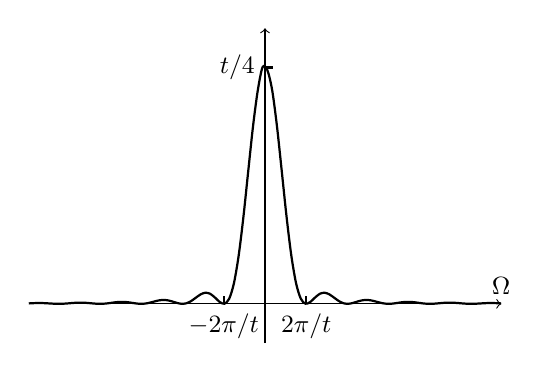
\begin{tikzpicture}
            \draw[->] (0,-0.5)--(0,3.5);
            \draw[->] (-3,0)--(3,0)node[above]{\small\(\Omega\)};
            \draw[domain=-3:3, smooth, variable=\x,samples=100,thick] plot ({\x}, {(sin(6*\x r))^2/(12*\x*\x)});
            \draw[thick] (0,3)node[left]{\small \(t/4\)}--(0.1,3);
            \draw[thick] (0.524,0)node[below]{\small \(2\pi/t\)}--(0.524,0.1);
            \draw[thick] (-0.524,0)node[below]{\small \(-2\pi/t\)}--(-0.524,0.1);
        \end{tikzpicture}
        \caption{A plot of \(\sin^2(\Omega t/2)/\Omega^2 t\) as a function of \(\Omega\) for fixed \(t\). It \(\to\pi\delta(\Omega)/2\) as \(t\to\infty\).}
        \label{Fig:Const_Per}
    \end{figure}

    Consider the graph of \(\sin^2(\Omega t/2)/\Omega^2\) as a function of \(\Omega\) for fixed \(t\), as shown in \cref{Fig:Const_Per} (Note that the plot has an extra \(t\) in the denominator.). The height of the central peak is \(\sim t^2\) while its width is \(\sim 1/t\), where we recall that \(t\) is the time over which the perturbation acted. For large \(t\), \(\abs{a_k(t)}^2\) is only appreciable for states \(k\) whose energies obey
    \begin{equation}
        t\sim\frac{2\pi}{\abs{\omega_{km}}}=\frac{2\pi\hbar}{\abs{E_k-E_m}}\,.
    \end{equation}
    In other words, if \(\Delta t\) is the time for which the perturbation has been switched on and \(\Delta E\) the energy difference between states which have an appreciable probability of a transition, then we require
    \begin{equation}
        \Delta t\Delta E\sim\hbar\,.
    \end{equation}
    For small \(\Delta t\), the central peak in \cref{Fig:Const_Per} is broad and we can have appreciable probability of a transition even between states with large \(\Delta E\). However, if the constant perturbation has been switched on for a long time, we will only obtain transitions to states \(\ket{k}\) that are (very nearly) degenerate with the original states \(\ket{m}\). In fact, as \(t\to\infty\), for \(\Omega\ne 0\) we have
    \begin{equation}
        \lim_{t\to\infty}\frac{\sin^2(\Omega t/2)}{\Omega^2 t}\le\lim_{t\to\infty}\frac{1}{\Omega^2 t}=0\,,
    \end{equation}
    whilst
    \begin{equation}
        \lim_{\Omega\to 0}\frac{\sin^2(\Omega t/2)}{\Omega^2 t}=\frac{t}{4}
    \end{equation}
    which diverges if we then send \(t\to\infty\). Furthermore, the integral of this function is
    \begin{equation}
        \int_{-\infty}^{\infty}\dd{\Omega}\frac{\sin^2(\Omega t/2)}{\Omega^2 t}=\frac{\pi}{2}\,,
    \end{equation}
    independent of \(t\). This shows that we can replace
    \begin{equation}
        \lim_{t\to\infty}\frac{\sin^2(\Omega t/2)}{\Omega^2 t}=\frac{\pi}{2}\delta(\Omega)\,,
    \end{equation}
    so that as \(t\to\infty\), the transition probability behaves as
    \begin{equation}
        \abs{a_k(t)}^2\sim\frac{2\pi}{\hbar^2}\abs{\mel{k}{\Delta}{m}}^2\delta(\omega_{km})t\,.
    \end{equation}
    We define the \textit{transition rate} \(\Gamma(m\to k)\) by
    \begin{equation}
        \Gamma(m\to k)=\lim_{t\to\infty}\pdv{}{t}\abs{a_k(t)}^2\,.
    \end{equation}
    In the case of a constant perturbation switched on at \(t=0\), we thus have
    \begin{equation}
        \Gamma(m\to k)=\frac{2\pi}{\hbar}\abs{\mel{k}{\Delta}{m}}^2\delta(E_k-E_m)\,,
    \end{equation}
    where we have written the argument of the \(\delta\)-function in terms of energies, pulling out a factor of \(\hbar\). As claimed, for this constant perturbation we only have a non-zero transition rate to states which are degenerate with our initial state.

    \subsection{Fermi's Golden Rule}
    Just a small extension of the above gives us one of the most important cases of time dependent perturbation theory. Suppose our perturbation takes the form
    \begin{equation}
        \Delta(t)=\begin{cases}
            0 & \text{for }t<0\\
            \Delta \ee^{-\ii \omega t}+\Delta^\dagger \ee^{+\ii \omega t} & \text{for }t>0\,,
        \end{cases}
    \end{equation}
    where again \(\Delta=\Delta(X,P,\dots)\) is some time-independent operator. Thus, as before our Schr\"{o}dinger picture perturbation \(\Delta(t)\) is turned on at \(t=0\), but thereafter it now oscillates with fixed frequency \(\omega\). Since \(\Delta(t)\) appears as a term in the Hamiltonian, it must be Hermitian, so we've included both an \(\ee^{+\ii \omega t}\) and \(\ee^{-\ii \omega t}\) term and without loss of generality we may take \(\omega>0\). We'll see below that these two terms are responsible for different physics. We call such perturbations \textit{monochromatic} in anticipation of the case that they describe an applied electromagnetic field, corresponding to light of frequency \(\omega\).

    We'll again consider the case where our system is initially in the \(m^{\text{th}}\) eigenstate of the unperturbed \(H_0\), so that \(a_n(0)=\delta_{nm}\). Performing the time integral in (\ref{TDPT_transition_amplitude}) in this monochromatic case is again trivial and yields
    \begin{equation}
        a_k(t)=\frac{\mel{k}{\Delta}{m}}{\hbar(\omega_{km}-\omega)}\left[\ee^{\ii (\omega_{km}-\omega)t}-1\right]+\frac{\mel{k}{\Delta^\dagger}{m}}{\hbar(\omega_{km}+\omega)}\left[\ee^{\ii (\omega_{km}+\omega)t}-1\right]\,.
    \end{equation}
    This is very similar to our result (\ref{constant_perturbation_ak}) for the constant perturbation, with the time-dependence of the perturbation just causing \(\omega_{km}\) to be replaced by \(\omega_{km}\pm\omega\). Consequently, we will obtain significant transitions amplitudes only to states \(\ket{m}\) for which \(E_k-E_m\approx\hbar\omega\), or else for which \(E_k-E_m\approx-\hbar\omega\) to high accuracy. The first situation, where \(E_k>E_m\approx\hbar\omega\) corresponds to our system \textit{absorbing} energy from the perturbation, whilst the second is \textit{stimulated emission} where the system is prompted to release energy by the perturbation. In this way, the time dependent monochromatic perturbation can be regarded as an enormous source and sink of energy that can be exchanged with the system.

    In the case of absorption, the first term dominates at late times. Thus the probability that the perturbation excites the system from \(\ket{m}\to\ket{k}\) is
    \begin{equation}
        \abs{a_k(t)}^2=\frac{4\abs{\mel{k}{\Delta}{m}}^2}{\hbar(\omega_{km}-\omega)^2}\sin^2\left(\frac{\omega_{km}-\omega}{2}t\right)
    \end{equation}
    with \(E_k>E_m\), correct to order \(\abs{\Delta}^2\). Replacing the late-time behaviour of \(\abs{a_k(t)}^2\) by a \(\delta\)-function as before shows that the transition rate is
    \begin{equation}\label{Fermi_golden_rule_abs}
        \Gamma(m\to k)=\lim_{t\to\infty}\pdv{}{t}\abs{a_k(t)}^2=\frac{2\pi}{\hbar}\abs{\mel{k}{\Delta}{m}}^2\delta(E_k-E_m-\hbar\omega)
    \end{equation}
    in the case that the system absorbs energy from the perturbation. In the opposite case that the system loses energy back into the perturbation, we have \(E_k<E_m\) and the corresponding transition rate is
    \begin{equation}\label{Fermi_golden_rule_emi}
        \Gamma(m\to k)=\frac{2\pi}{\hbar}\abs{\mel{m}{\Delta}{k}}^2\delta(E_k-E_m+\hbar\omega)
    \end{equation}
    with an opposite sign in the \(\delta\)-function. These results were first obtained by Dirac. They proved to be so useful in describing atomic transitions that Fermi dubbed them `golden rules'. The name stuck and now (\ref{Fermi_golden_rule_abs}) and (\ref{Fermi_golden_rule_emi}) are known as Fermi's golden rule.

    On the one hand, we may be interested not in transitions to some specific final state \(\ket{k}\), but to any one of a range of continuum eigenstates of \(H_0\). A typical example here would be transitions between an initial bound state of an atom to any of the continuum of positive-energy (non-bound) states. In these circumstances, we let \(n(E_k)\d{E_k}\) denote the number of states with energy in the interval \((E_k,E_k+\delta E_k)\). The function \(n(E_k)\) --- which needs to be calculated in each case --- is known as the \textit{density of states}; note that it must have dimensions of \(1/(\text{energy})\) in order for \(n(E_k)\d{E_k}\) to be a number of states. The total transition probability from \(\ket{m}\) is then \(\int\dd{E_k}\abs{a_k(t)}^2 n(E_k)\), generalizing the sum \(\sum_k \abs{a_k(t)}^2\) in the discrete case. In particular, in the case of absorption the total transition rate from our initial eigenstate \(\ket{m}\) is given by
    \begin{align}
        \int\dd{E_k}\Gamma(m\to k)n(E_k)&=\frac{2\pi}{\hbar}\int\dd{E_k}\abs{\mel{k}{\Delta}{m}}^2\delta(E_k-E_m-\hbar\omega)n(E_k)\\
        &=\frac{2\pi}{\hbar}\abs{\mel{k}{\Delta}{m}}^2\left.n(E_k)\right|_{E_k=E_m+\hbar\omega}
    \end{align}
    to lowest non-trivial order in perturbation theory. We see that we always make transitions through an energy of exactly \(\hbar\omega\), with the density of states telling us how many states of energy \(E_m+\hbar\omega\) there actually are.

    On the other hand, Fermi's golden rule is also useful when our perturbation itself contains a continuum of different frequencies, perhaps thought of as a Laplace or Fourier transform of some a perturbation with generic time dependence. In this case, transitions between discrete bound states are generally possible, because there will always be some perturbation at exactly the right frequency \(\omega=\omega_{km}=(E_k-E_m)/\hbar\), even though the right-hand side takes discrete values as \(k\) varies over different bound states as the final state.

    Let's now consider an example of each of these two cases.

    \subsubsection{The Photoelectric Effect}
    First, we'll use Fermi's golden rule to calculate the rate at which an applied monochromatic electromagnetic field can ionize an atom, say hydrogen, stripping off the electron from a bound state into the continuum of ionized states. We'll assume that the electromagnetic field itself may be treated classically --- this assumption is valid e.g. in a laser, or at the focus of the antenna of a radio telescope where the field is large. Of course, if we wish perturbation theory to produce reliable results, we'll still need this applied electromagnetic field to be small compared to the Coulomb fields binding the electron(s) to the nucleus of the atom.

    In the vacuum, the electromagnetic field is divergence free and is entirely generated by Faraday's Law \(\curl\vb{E}=-\partial\vb{B}/\partial t\). The whole electromagnetic field can be described by a vector potential \(\vb{A}\) via
    \begin{equation}
        \vb{b}=\curl\vb{A}\quad\text{and}\quad\vb{E}=-\frac{1}{c}\pdv{\vb{A}}{t}\,.
    \end{equation}
    In the monochromatic case, Faraday's equation is solved by
    \begin{equation}
        \vb{A}(\vb{x},t)=\vb{\epsilon}\cos(\vb{k}'\vdot\vb{x}-\omega t)\,,
    \end{equation}
    where \(\vb{\epsilon}\) is a constant vector describing the polarization of the wave and \(\vb{k}'\) is the wavevector. (we reserve \(\vb{k}\) for later use.) From the vacuum Maxwell equation \(\div\vb{E}=0\), we learn that
    \begin{equation}\label{transverse}
        \vb{k}'\vdot\vb{\epsilon}=0\,,
    \end{equation}
    saying that the wave is transverse. Faraday's law then reduces to the statement that \(\omega=c\abs{\vb{k}'}\) so that the wave travels at the speed of light.

    The coupling of an elementary particle of charge \(q\) to such a vector potential is given by the minimal coupling rule, replacing
    \begin{equation}
        \vb{P}\longmapsto\vb{P}-q\vb{A}(\vb{X},t)
    \end{equation}
    in the Hamiltonian\footnote{This is called minimal coupling because more complicated modifications are possible if the charged particle is not elementary, or in other more complicated circumstances. You'll learn more about this in the Part II Classical Dynamics and Applications of Quantum Mechanics.}, so
    \begin{equation}
        H=\frac{(\vb{P}-q\vb{A})^2}{2\mu}+V(\vb{X})=H_0-\frac{q}{2\mu}(\vb{P}\vdot\vb{A}-\vb{A}\vdot\vb{P})+\frac{q^2\vb{A}^2}{2\mu}\,,
    \end{equation}
    where \(H_0\) contains the original potential term \(V(\vb{X})\) as well as the kinetic term. In our case of atomic transitions, an electron has charge \(q=e\) so to first order in \(e\) the perturbing Hamiltonian is
    \begin{equation}
        \Delta(t)=\frac{e}{2\mu}\left(\vb{P}\vdot\vb{\epsilon}\cos(\vb{k}'\vdot\vb{X}-\omega t)+\cos(\vb{k}'\vdot\vb{X}-\omega t)\vb{\epsilon}\vdot\vb{P}\right)\,.
    \end{equation}
    The component \(\vb{\epsilon}\vdot\vb{P}\) of the momentum operator in the direction of the polarization of the electromagnetic wave commutes with \(\cos(\vb{k}'\vdot\vb{X}-\omega t)\) by the transversality condition (\ref{transverse}) (recall that \(\vb{\epsilon}\) itself is a constant vector). Thus
    \begin{align}
        \Delta(t)&=\frac{e}{\mu}\cos(\vb{k}'\vdot\vb{X}-\omega t)\vb{\epsilon}\vdot\vb{P}\notag\\
        &=\frac{e}{2\mu}(\ee^{\ii (\vb{k}'\vdot\vb{X}-\omega t)}+\ee^{-\ii (\vb{k}'\vdot\vb{X}-\omega t)})\vb{\epsilon}\vdot\vb{P}\,.\label{photoelectric_perturbation}
    \end{align}

    Having found the form of our perturbation, we now need calculate its matrix element between our initial and final states. We'll consider the case where the hydrogen atom is initially in its ground state, so that \(m=\ket{1,0,0}\) with position space wavefunction
    \begin{equation}
        \psi_0(\vb{x})=\braket{\vb{x}}{1,0,0}=\frac{1}{\sqrt{\pi a_0^3}}\ee^{-r/a_0}\,,
    \end{equation}
    where \(a_0\) is the Bohr radius. For the final state, we are interested in the case where the electron has been liberated from the proton. If the energy of the ejected electron is sufficiently great, we can ignore its Coulomb attraction back to the ion and treat the final electron as a free particle of momentum \(\hbar\vb{k}\), so we take our final state \(\ket{\vb{k}}\) to be the plane-wave
    \begin{equation}
        \psi_{\vb{k}}(\vb{x})=\braket{\vb{x}}{\vb{k}}=\frac{1}{(2\pi\hbar)^{3/2}}\ee^{\ii \vb{k}\vdot\vb{x}}\,.
    \end{equation}
    This transition requires that the electron absorbs energy from the radiation, so the matrix element we seek comes from the first term of the perturbation Hamiltonian (\ref{photoelectric_perturbation}). We have
    \begin{align}
        \mel{\vb{k}}{\Delta}{100}&=\frac{e}{2\mu}\mel{\vb{k}}{\ee^{\ii \vb{k}'\vdot\vb{X}}\vb{\epsilon}\vdot\vb{P}}{1,0,0}\notag\\
        &=-\frac{\ii\hbar e}{2\mu}\frac{1}{(2\pi\hbar)^{3/2}(\pi a_0^3)^{1/2}}\int_{\RR^3}\dd[3]{\vb{x}}\ee^{-\ii \vb{k}\vdot\vb{x}}\ee^{\ii \vb{k}'\vdot\vb{x}}\vb{\epsilon}\vdot\grad(\ee^{-r/a_0})\,.
    \end{align}
    Integration by parts and using the fact that the bound state wavefunction decays exponentially as \(\abs{\vb{x}}\to\infty\), this is
    \begin{equation}
        \mel{\vb{k}}{\Delta}{1,0,0}=\frac{e\hbar}{2\mu}\frac{\vb{\epsilon}\vdot\vb{k}}{(2\pi\hbar)^{3/2}(\pi a_0^3)^{1/2}}\int_{\RR^3}\dd[3]{\vb{x}}\ee^{-\ii \vb{q}\vdot\vb{x}}\ee^{-r/a_0}\,,
    \end{equation}
    where \(\vb{q}=\vb{k}-\vb{k}'\) is the momentum transfer and we recall that the polarisation vector is transverse, \(\vb{\epsilon}'\vdot\vb{k}'=0\). We're left with just the Fourier transform of the ground state wavefunction. Choosing the \(z\)-axis to lie along the direction of \(\vb{q}\) and working in polar coordinates, this is
    \begin{equation}
        \int\dd[3]{\vb{x}}\ee^{-\ii \vb{q}\vdot\vb{x}}\ee^{-r/a_0}=\frac{4\pi}{q}\int_{0}^{\infty}\dd{r}r \ee^{-r/a_0}\sin(qr)=\frac{8\pi a_0^3}{(1+a_0^2q^2)^2}\,,
    \end{equation}
    where \(q=\abs{\vb{q}}\).

    We now wish to use this matrix element in Fermi's golden rule for the transition rate. Since there are a range of possible final momenta, we define the differential rate \(\Gamma_{\ket{1,0,0}\to\vb{k}}\) to be the rate at which the radiation ionizes an atom so that the momentum of the ejected electron lies in the range \(\hbar(\vb{k},\vb{k}+\delta k)\), so
    \begin{align}
        \d{\Gamma_{\ket{1,0,0}\to\ket{\vb{k}}}}&=\frac{2\pi}{\hbar}\abs{\mel{\vb{k}}{\Delta}{1,0,0}}^2\delta(E_{\vb{k}}-E_{100}-\hbar\omega)\hbar^3\d[3]{\vb{k}}\notag\\
        &=2\pi\hbar^2\abs{\mel{\vb{k}}{\Delta}{1,0,0}}^2\delta(E_{\vb{k}}-E_{100}-\hbar\omega)\,\dd{\Omega}k^2\dd{k}\,,
    \end{align}
    where \(\d{\Omega}=\sin\theta\d{\theta}\d{\phi}\). To relate this differential rate to our previous expression for the rate of transition into states of particular energy, recall that we're treating the final electron as a free particle, so its energy is \(E_{\vb{k}}=\hbar^2\vb{k}^2/2\mu\). Thus we have
    \begin{equation}
        k^2\d{k}=k^2\left(\dv{E_k}{k}\right)^{-1}\d{E_k}=\left(\frac{\mu k}{\hbar^2}\right)\d{E_k}\,,
    \end{equation}
    so for a free particle, the density of states \(n(E_k)=\mu k/\hbar^2=\mu\sqrt{2\mu E_k}/\hbar^3\). Putting all the pieces together and integrating over the final state energy, the transition rate for electrons to be emitted into the direction \(\d{\Omega}\) of solid angle is
    \begin{equation}
        \dv{\Gamma_{\ket{1,0,0}\to\ket{\vb{k}}}}{\Omega}=\frac{4e^2(ka_0)^3}{\pi\mu\hbar}\frac{\abs{\vb{\epsilon}\vdot\vu{k}}^2}{(1+a_0^2q^2)^4}\,,
    \end{equation}
    where \(\hbar k=\sqrt{2\pi E_k}\) is frozen to \(\sqrt{2\pi(\hbar\omega+E_{100})}\approx\sqrt{2\mu\hbar\omega}\).

    \subsubsection{Absorption and Stimulated Emission}
    Now let's consider the case where instead of being illuminated by monochromatic light such as from a laser, our atom is immersed in a bath of thermal radiation. This radiation bath supplies us with a continuous range of different frequencies, so transitions between different (discrete) bound states of the atom are now possible.

    The problem simplifies if we assume that the typical electromagnetic wavelength \(1/k'\) in the thermal bath is much larger than the Bohr radius of the atom. This is a good approximation provided the atomic transition occurs between states that are separated in energy by much less than \(\alpha\mu c^2\), as will be the case for transitions between highly excited energy levels, perhaps by the valence electrons in a heavy atom. Such wavelengths correspond to radiation with frequencies that are less than those of soft X-rays. In this approximation, \(\vb{k}'\vdot\vb{X}\ll 1\) for all locations in the atom or molecule at which there is significant probability of finding the electron. To lowest order, we can thus approximate the electric field as being constant over the scale of the atom. The Hamiltonian for the atom is then
    \begin{equation}
        H=H_0+e\sum_r \vb{E}(t)\vdot\vb{X}_r\,,
    \end{equation}
    where \(H_0\) is the Hamiltonian of the unperturbed atom, \(\vb{E}(t)\) is the fluctuating electric field due to the radiation and \(\vb{X}_r\) is the position operator for the \(r^{\text{th}}\) electron in the atom. This is known as the \textit{dipole approximation} since the operator \(e\sum_r \vb{X}_r\) represents the atom's dipole moment. We interpret the transition as occurring due to the interaction between the applied electric field and this dipole.

    Whilst roughly constant over the atom, the electric field \(\vb{E}(t)\) fluctuates rapidly in time as the atom is jostled by radiation of different frequencies in the thermal bath. In particular, on average \(\overline{\vb{E}(t)}=0\) since the electric field is equally likely to point in any direction at any given moment. We take \(\vb{E}(t)\) to be correlated as
    \begin{equation}\label{E_field_correlation}
        \overline{E_i(t_1)E_j(t_2)}=\delta_{ij}\int_{\RR}\dd{\omega}\mathcal{P}(\omega)\ee^{-\ii \omega(t_1-t_2)}\,.
    \end{equation}
    The presence of \(\delta_{ij}\) means that the fluctuation in different directions are uncorrelated, whilst fluctuations that are aligned are correlated equally no matter their direction. This just says that there is no preferred direction for the electric field and holds e.g. for a thermal bath of radiation.

    We can understand the meaning of the function \(\mathcal{P}(\omega)\) as follows. First, note that if the electric fields are real, then we must have
    \begin{equation}\label{P_conditions}
        \mathcal{P}(-\omega)=\mathcal{P}(\omega)\quad\text{and}\quad\mathcal{P}(\omega)^*=\mathcal{P}(\omega)
    \end{equation}
    so that \(\mathcal{P}\) is a real, even function. Recall from IB electromagnetism that the energy density of an electromagnetic field is
    \begin{equation}
        \frac{\epsilon_0}{2}(\vb{E}^2(\vb{x},t)+c^2\vb{B}^2(\vb{x},t))
    \end{equation}
    and in purely radiative (source-free) field \(\vb{E}^2=c^2\vb{B}^2\). In our case, (\ref{E_field_correlation}) shows that the average energy density we expect to find in the radiation at time \(t\) is
    \begin{equation}
        \epsilon_0\overline{E_i(t)E_i(t)}=3\epsilon_0\int_{-\infty}^{\infty}\dd{\omega}\mathcal{P}(\omega)=6\epsilon_0\int_{0}^{\infty}\dd{\omega}\mathcal{P}(\omega)
    \end{equation}
    so \(\rho(\omega)=6\epsilon_0\mathcal{P}(\omega)\) represents the average energy density in radiation at energy time due to frequencies in the range \((\omega,\omega+\d{\omega})\). (If the radiation is truly thermal at temperature \(T\), then \(\rho(\omega)\) would be given by the Planck's blackbody formula
    \begin{equation}
        \rho(\omega)=\frac{\hbar\omega^3}{\pi^3 c^2}\frac{1}{\ee^{-\hbar\omega/k_B T}-1}
    \end{equation}
    coming from the Bose--Einstein distribution. You'll learn about this in the Statistical Physics course.)

    Now let's put these results to work. For a transition \(\ket{m}\to\ket{k}\), we have
    \begin{equation}
        a_k(t)=-\frac{ie}{\hbar}\int_{0}^{t}\dd{t'}\sum_{r}\mel{k}{\vb{E}(t')\vdot\vb{X}_r}{m}\ee^{\ii \omega_{km}t'}\,.
    \end{equation}
    We write the probability that the atom is found in state \(\ket{k}\) at time \(t\) as a double integral
    \begin{equation}
        \abs{a_k(t)}^2=\frac{e^2}{\hbar^2}\int_{0}^{t}\int_{0}^{t}\dd{t_1}\dd{t_2}\sum_{r,r'}\mel{k}{\vb{E}(t_1)\vdot\vb{X}_{r'}}{m}\mel{m}{\vb{E}(t_2)\vdot\vb{X}_{r}}{k}\ee^{\ii \omega_{km}(t_1-t_2)}\,.
    \end{equation}
    The correlation (\ref{E_field_correlation}) in our thermal bath shows that, on average,
    \begin{align}
        \overline{\abs{a_k(t)}^2}&=\frac{e^2}{\hbar^2}\int_{0}^{t}\int_{0}^{t}\dd{t_1}\dd{t_2}\overline{E_i(t_1)E_j(t_2)}\sum_{r,r'}\mel{k}{(X_{r'})_i}{m}\mel{m}{(X_r)_j}{k}\ee^{\ii \omega_{km}(t_1-t_2)}\notag\\
        &=\frac{e^2}{\hbar^2}\abs{\sum_r\mel{k}{\vb{X}_r}{m}}^2\times\int_{-\infty}^{\infty}\dd{\omega}\mathcal{P}(\omega)\int_{0}^{t}\int_{0}^{t}\dd{t_1}\dd{t_2}\ee^{\ii (\omega_{km}-\omega)(t_1-t_2)}\notag\\
        &=\frac{e^2}{\hbar^2}\abs{\sum_r\mel{k}{\vb{X}_r}{m}}^2\times\int_{-\infty}^{\infty}\dd{\omega}\mathcal{P}(\omega)\abs{\int_{0}^{t}\dd{t_1}\ee^{\ii (\omega_{km}-\omega)t_1}}^2\notag\\
        &=\frac{4e^2}{\hbar^2}\abs{\sum_r\mel{k}{\vb{X}_r}{m}}^2\times\int_{-\infty}^{\infty}\dd{\omega}\mathcal{P}(\omega)\frac{\sin^2\left(\frac{(\omega_{km}-\omega)t}{2}\right)}{(\omega_{km}-\omega)^2}\,,
    \end{align}
    where the mod-square includes the Euclidean inner product of the two \(\mel{k}{\vb{X}_r}{m}\) matrix elements. This form is again familiar, except that instead of a density of final states, we have \(\mathcal{P}(\omega)\), representing the average density \(\rho(\omega)\) of the frequency \(\omega\) component of the radiation. Making our familiar placement, and performing the integral over \(\omega\) using the resulting \(\delta\)-function in the \(t\to\infty\) limit, we have the transition rate
    \begin{equation}\label{atom_transition_rate}
        \Gamma(\ket{m}\to\ket{k})=\frac{\pi e^2}{3\epsilon_0\hbar^2}\abs{\sum_r \mel{k}{\vb{X}_r}{m}}^2\rho(\omega_{km})\,.
    \end{equation}
    in the case that the states \(\ket{m}\) and \(\ket{k}\) are discrete but we have a continuous range of perturbing frequencies.

    This result is very intuitive: the rate of transition depends on the probability that the dipole moment transition can link states \(\ket{m}\) and \(\ket{k}\), together with the energy density in the radiation bath at the right frequency to match this transition. For hydrogenic states of the atom, we recall that the matrix element vanishes unless the selection rules
    \begin{equation}
        \abs{\ell-\ell'}=1\quad\text{and}\quad\abs{m-m'}\le 1
    \end{equation}
    are obeyed. These selection rules were derived under the assumption that the transition is just due to the dipole approximation where the perturbation involves matrix elements of the dipole moment operator \(e\vb{X}\). The effects of both higher orders in perturbation theory, and inclusion of interactions beyond those of an electric field with wavelength \(\lambda\gg a_0\) mean that transitions that are `forbidden' according to the above selection rules may in fact occur. They will typically do so, however, at a much smaller rate.

    Now, whether or not the radiation bath is thermal, the reality conditions (\ref{P_conditions}) show that the rate \(\Gamma(\ket{m}\to\ket{k})\) in (\ref{atom_transition_rate}) is an even function of \(\omega_{km}\). Consequently, for fixed \(\abs{E_k-E_m}\), this rate is the same whether \(E_k>E_m\) or \(E_k<E_m\). For \(E_k>E_m\), the atom absorbs energy from the radiation, exciting to a higher energy level, whilst if \(E_k<E_m\) the atom emits energy back into the radiation as it decays to a lower energy state. The important result we've obtained is that the rate for stimulated emission is the same as the rate of absorption.
    
    \subsubsection{Spontaneous Emission}
    Our treatment above calculated the rate at which an atom would decay (or excite) due to being immersed in a bath of radiation. However, we currently cannot understand decays of an isolated atom: if the atom is prepared in any eigenstate of \(H_0\), quantum mechanics says that in the absence of a perturbation it will just stay there. Remarkably, Einstein was able to relate the rate of spontaneous decay of an atom to the rate of stimulated decay that we calculated above.

    Suppose our atom is immersed in a bath of radiations where the energy density of photons with frequency in the range \((\omega+\d{\omega})\) is \(\rho(\omega)\dd{\omega}\). Einstein defined \(A_{m\to k}(\omega_{mk})\) as the rate at which an atom would spontaneously decay from a state of energy \(E_m\) to a state of lower energy \(E_k\), where \(\omega_{mk}=(E_m-E_k)/\hbar\) is the frequency of the emitted photon. We let \(\rho(\omega_{km}) B_{k\to m}(\omega_{km})\) denote the rate at which energy is absorbed from the radiation bath, exciting the atom from \(\ket{k}\) to \(\ket{m}\). Similarly, let \(\rho(\omega_{km})B_{m\to k}(\omega_{km})\) denote the rate of decay of the excited atom due to stimulation by the presence of the radiation bath. We calculated \(B_{m\to k}\) and \(B_{k\to m}\) in the dipole approximation above, finding they were the same, but let's pretend that (like Einstein) we don't know this yet.

    In thermodynamic equilibrium these rates must balance, so if there are \(n_k\) atoms in state \(\ket{k}\) and \(n_m\) in state \(\ket{m}\), we must have
    \begin{equation}\label{rate_equilibrium}
        n_m(A_{m\to k}(\omega_{mk})+\rho(\omega_{km})B_{m\to k}(\omega_{km}))=n_k\rho(\omega_{km})B_{k\to m}(\omega_{km})\,.
    \end{equation}

    We will borrow two results you will derive in Part II Statistical Physics. First, when a gas of atoms is in equilibrium at temperature \(T\), the relative numbers of atoms in states with energies \(E_m\) and \(E_k\) is given by the \textit{Boltzmann distribution}
    \begin{equation}
        \frac{n_k}{n_m}=\frac{\ee^{-E_k/k_B T}}{\ee^{-E_m/k_B T}}=\ee^{\hbar\omega_{mk}/k_B T}\,,
    \end{equation}
    where \(k_B\approx 1.38\times 10^{-23}\unit{J}\unit{K}^{-1}\) is the \textit{Boltzmann's constant}. Furthermore, if radiation is in equilibrium at the same temperature then the density of states of photons at frequency \(\omega\) is
    \begin{equation}
        \rho(\omega)=\frac{\hbar\omega^3}{\pi^2 c^3}\frac{1}{\ee^{\hbar\omega_{mk}/k_B T}-1}\,,
    \end{equation}
    which is essentially the Bose--Einstein distribution. Using these in (\ref{rate_equilibrium}) gives
    \begin{equation}
        A_{m\to k}(\omega)=\frac{\hbar\omega^3}{\pi^2 c^3}\frac{1}{\ee^{\hbar\omega/k_B T}-1}\left(\ee^{\hbar\omega/k_B T}B_{k\to m}(\omega)-B_{m\to k}(\omega)\right)\,,
    \end{equation}
    where \(\omega=\omega_{m\to k}\). However, \(A_{m\to k}\) is supposed to be the rate of spontaneous emission of radiation from the atom, so it cannot depend on any properties of the radiation bath. In particular, it must be independent of the temperature \(T\). This is possible iff
    \begin{equation}
        B_{k\to m}(\omega)=B_{m\to k}(\omega)\,,
    \end{equation}
    so that the rates of stimulated emission and absorption agree. In this case, we have
    \begin{equation}
        A_{m\to k}(\omega)=\frac{\hbar\omega^3}{\pi^2 c^3}B_{m\to k}(\omega)
    \end{equation}
    so that knowing the rate \(B_{k\to m}\ket{\omega}\) at which a classical electromagnetic wave of frequency \(\omega=(E_m-E_k)/\hbar\) is absorbed by an atom, we can also calculate the rate \(A_{m\to k}(\omega)\) at which the atom spontaneously decays, even in the absence of radiation.

    Now we have found from first-principle calculations that
    \begin{equation}
        \Gamma(\ket{m}\to\ket{k})=\frac{\pi e^2}{3\epsilon_0\hbar^2}\abs{\sum_r\mel{k}{\vb{X}_r}{m}}^2\rho(\omega_{km})
    \end{equation}
    in the dipole approximation, to first-order in perturbation theory. Consequently, for our atom Einstein's \(B\) coefficient is
    \begin{equation}
        E_{k\to m}(\omega_{km})=B_{m\to k}(\omega_{km})=\frac{\pi e^2}{3\epsilon_0\hbar^2}\abs{\sum_r\mel{k}{\vb{X}_r}{m}}^2
    \end{equation}
    for stimulated emission or absorption. From Einstein's statistical argument we thus learn that
    \begin{equation}\label{Einstein_A_coeff}
        A_{m\to k}(\omega)=\frac{e^2\omega^3}{3\epsilon_0\pi\hbar c^3}\abs{\sum_r\mel{k}{\vb{X}_r}{m}}^2
    \end{equation}
    is the rate at which an excited atom must spontaneously decay, even in the absence of any applied radiation.

    Ingenious though it is, there's something puzzling about this calculation of the rate of spontaneous decay. Where does our quantum mechanical calculation stating that isolated excited atoms do not decay go wrong? The answer is that while we treated the energy levels of the atom fully quantum mechanically, the electromagnetic field itself was treated classically. Spontaneous emission is only possible once one also quantizes the electromagnetic field, since it is fluctuations in the zero-point value of this field that allow the atom to emit a photon and decay; heuristically, the fluctuating value of the quantum electromagnetic field --- even in the vacuum --- `tickles' the excited atom prompting the decay. Treating the EM field classically is appropriate if the radiation comes from a high intensity laser, where the energy density of the field is so high that the terms \(B(\omega)\rho(\omega)\) dominate in (\ref{rate_equilibrium}). By contrast, emission of light from the atoms in a humble candle is an inherently quantum phenomenon, occurring purely by spontaneous emission once the flame is lit --- candlelight shines even in ambient darkness.

    Einstein gave his statistical argument in 1916, when Bohr's model of the atom (the first thing you met in IB QM) was still the deepest understanding physicists had of quantum theory. This was at the same time as he was revolutionising our understanding of gravity, space and time, which obviously wasn't enough to keep him fully occupied. The quantum treatment of stimulated emission given in the previous section is due to Dirac in 1926, the same year as Schr\"{o}dinger first published his famous equation. A first principles calculation of the spontaneous emission rate \(A_{m\to k}\), requiring the quantization of the electromagnetic field, was also given by Dirac just one year later. Things move fast. Dirac's 1927 results agreed with those we've found via Einsteins argument. The necessity also to quantize the electromagnetic field heralded the arrival of Quantum Field Theory.

    Let's use these results to calculate the typical lifetime of an excited state of an isolated atom. When the radiation density \(\rho(\omega)\) is very small, the number of atoms \(n_m\) in the excited state obeys
    \begin{equation}
        \pdv{n_m}{t}=-A_{m\to k}n_m
    \end{equation}
    so the atom decays exponentially with a characteristic timescale \(\sim A_{m\to k}^{-1}\). For hydrogen or an alkali atom, typically the outermost electron changes its energy level in the transition, so we can drop the sum in (\ref{Einstein_A_coeff}) to find
    \begin{equation}
        A_{m\to k}(\omega)=\frac{e^2\omega^3}{3\pi\epsilon_0\hbar c^3}\abs{\mel{k}{\vb{X}}{m}}^2
    \end{equation}
    where \(\vb{X}\) is the position of the outermost electron. Unless \(\mel{k}{X}{m}\) vanishes due to some selection rule, we'd expect this matrix element to be of the typical size \(a_0=4\pi\epsilon_0\hbar^2/\mu e^2\) characteristic of the atom, so \(\abs{\mel{k}{X}{m}}^2\sim a_0^2\). Hence the characteristic lifetime of the
    excited atomic state is roughly
    \begin{equation}
        \tau=A_{m\to k}^{-1}\sim\frac{3\pi\epsilon_0\hbar c^3}{e^2\omega^3 a_0^2}=\frac{3\mu c^3}{4\hbar\omega^3 a_0}
    \end{equation}
    where \(\mu\) is the mass of the electron. Optical light has a frequency of order \(\omega\sim 10^{15}\unit{Hz}\) so the timescale \(\tau\) is around \(10^7\) times longer than the timescale \(E_{200}\) associated with the energy \(E_{200}\) of the first excited state of hydrogen. Thus around \(10^7\) oscillations of the hydrogen atom occur before it radiates a photon, decaying down into the ground state.

    \newpage
    \section{Interpreting Quantum Mechanics}\label{Chap:Interpreting_QM}
    In this final chapter, we will explore the process of \textit{measurement} in quantum mechanics. According to the Copenhagen interpretation, when we perform a measurement the state of the particle collapses onto an eigenstate of the corresponding operator, with the probability of different results being given by the Born rule (\ref{Born_rule}). This entails a departure from the unitary (and hence deterministic) time evolution of our system as described by Schr\"{o}dinger's equation. However, the Copenhagen interpretation does not tell us exactly what physical process should count as a `measurement': does the observer need to be alive? to be human? to have taken PQM? Without such a prescription, how can we know when it is appropriate to evolve our state as \(\ket{\psi(t)} = U(t) \ket{\psi(0)}\) and when instead it should collapse?

    A further problem with measurement is that the states we measure usually correspond to what we consider to be `classically sensible' quantities. This seems to imply that measurements involve a preferred choice of basis for the system's Hilbert space. To give a famous example, we are all familiar with living cats and dead cats, but no-one has ever seen a cat that is simultaneously alive + dead. But why should quantum mechanics distinguish the basis
    \begin{equation}
        \{\ket{\text{alive}},\ket{\text{dead}}\}\quad\text{over}\quad\left\{\frac{\ket{\text{alive}}+\ket{\text{dead}}}{\sqrt{2}},\frac{\ket{\text{alive}}-\ket{\text{dead}}}{\sqrt{2}}\right\}\,?
    \end{equation}
    In this chapter, we'll examine these issues from the perspective of \textit{decoherence}. The formalism presented here is completely standard, and indeed decoherence is an important, well-established property of any quantum system. However, the jury is still out on whether this finally resolves the infamous problems with measurement in quantum mechanics.

    \subsection{The Density Operator}
    To get started, we must first realise that during a measurement, we cannot treat our quantum system as being isolated. Any form of measurement requires that we bring the system under study into contact with some form of measuring apparatus. Up to this point, we've assumed that we know the precise quantum state our system is in. While this may be possible for a small, isolated quantum system, we cannot possibly hope to know the exact quantum state of a macroscopic measuring device, which may easily contain \(\sim10^{23}\) atoms. Thus, to talk about measurements, we first need a way to describe systems even when we're not sure which state they're in. In fact, even in purely classical systems, there's always some uncertainty in our knowledge of the system: we never actually know the momentum of a single particle with infinite precision even in classical mechanics, because all our measurements are subject to some experimental error.

    Let's now see how to incorporate such imprecision in our knowledge into quantum mechanics. Suppose we know only that our system is in one of the states \(\{\ket{\psi_\alpha}\}\), and that the probability it is in state \(\ket{\psi_\alpha}\) is \(p_\alpha\). It's important to be clear that we're not saying
    \begin{equation}
        \ket{\Psi}=\sum_\alpha\sqrt{p_\alpha}\ket{\psi_\alpha}
    \end{equation}
    because \(\ket{\Psi}\) itself is a well-defined quantum state. Rather, we're admitting that we don't know the true state of the system, which could be any of the states \(\{\ket{\psi_\alpha}\}\). Indeed, these states do not need to form a complete set, and do not even need to be orthogonal, although we will take them each to be correctly normalized \(\braket{\psi_\alpha}{\psi_\alpha}=1\) for each \(\alpha\).

    In this case, the average result we obtain when measuring the value of some observable \(Q\) is
    \begin{equation}\label{average_result}
        \overline{Q}=\sum_{\alpha}p_\alpha\expval{Q}{\psi_\alpha}\,.
    \end{equation}
    This expression combines the quantum expectation value of \(Q\) in the state \(\ket{\psi_\alpha}\) (which may not be an eigenstate of \(Q\)), together with our lack of knowledge of the system's state, represented by the \(p_\alpha\)'s. For future use,  it'll be convenient to describe this using a \textit{density operator} \(\rho:\hb\to\hb\), defined by
    \begin{equation}
        \rho=\sum_\alpha p_\alpha\ket{\psi_\alpha}\bra{\psi_\alpha}\,,
    \end{equation}
    where the \(p_\alpha\) are the probabilities introduced above. Then we can write the average (\ref{average_result}) as
    \begin{equation}
        \overline{Q}=\tr_\hb(\rho Q)\,.
    \end{equation}
    To see this, suppose \(\{\ket{q_n}\}\) is a complete set of eigenstates of \(Q\), with eigenvalues \(\{q_n\}\). Using \(\{\ket{q_n}\}\) as a basis for \(\hb\) we have
    \begin{align}
        \tr_\hb(\rho Q)&=\sum_n\expval{\rho Q}{q_n}=\sum_{n,\alpha}p_\alpha\braket{q_n}{\psi_\alpha}\mel{\psi_\alpha}{Q}{q_n}\notag\\
        &=\sum_{n,\alpha}p_\alpha q_n\abs{\braket{q_n}{\psi_\alpha}}^2=\sum_\alpha p_\alpha\expval{Q}{\psi_\alpha}\,.
    \end{align}

    The density operator has the following three properties: First, it is a Hermitian operator
    \begin{equation}
        \rho^\dagger=\rho,
    \end{equation}
    reflecting the fact that the probabilities \(p_\alpha\) must be real. Second,
    \begin{equation}
        \tr_\hb(\rho)=1
    \end{equation}
    since the probabilities sum to one, and third,
    \begin{equation}
        \expval{\rho}{\psi}\ge 0
    \end{equation}
    for all \(\ket{\psi}\in\hb\) since probabilities are non-negative. We often write this property as \(\rho\ge 0\) for short. In fact, these three properties can be taken to be the defining properties of a density operator, in the sense that any operator obeying these three properties is the density operator for some system. To see this, suppose the eigenvectors of \(\rho\) are \(\ket{\phi_r}\), with \(\rho\ket{\phi_r}=\rho_r\ket{\phi_r}\). Then since \(\rho=\rho^\dagger\) we have \(\rho_r\in R\). The remaining two properties tell us that \(\sum_r\rho_r=1\) and \(\rho_r\ge 0\). Any set of real numbers \(\rho_r\) obeying these conditions can be taken to be a probability distribution for some system. Note that since the \(\ket{\phi_r}\) are eigenvectors of the Hermitian operator \(\rho\), they're necessarily orthogonal, in contrast to the arbitrary set of states we used in (\ref{average_result}).

    If we have perfect knowledge of our system, meaning \(\rho=\ket{\psi}\bra{\psi}\) so that with probability 1 the system is in state \(\ket{\psi}\), then we refer to it as \textit{pure}. Correspondingly, if our knowledge of the state is incomplete, so that \(\rho=\sum_\alpha p_\alpha\ket{\psi_\alpha}\bra{\psi_\alpha}\) with more than one \(p_\alpha>0\), we say that the system is in an \textit{impure} or \textit{mixed} state. This terminology is somewhat misleading, because it is really just our knowledge that is incomplete --- the system itself is presumably in some perfectly well-defined quantum state, it's just that we don't know which one.

    The density operator and the operators for the Hamiltonian and other observables encapsulate a complete, self-contained theory of quantum dynamics. If we have incomplete knowledge of the system's quantum state, then use of this formalism is mandatory. If we do happen to know that our system is initially in the precise quantum state \(\ket{\psi}\), we can still use this apparatus by setting \(\rho=\ket{\psi}\bra{\psi}\), rather than using time dependent Schr\"{o}dinger's equation, though in this case use of the density operator is optional.

    \subsubsection{The Bloch Sphere}
    As a simple example, consider a single spin-\(\frac{1}{2}\) particle with \(\{\ket{\uparrow},\ket{\downarrow}\}\) forming a basis of \(\hb\cong\CC^2\). If we know for sure that the system is in the state \(\ket{\uparrow}\), then
    \begin{equation}
        \rho=\ket{\uparrow}\bra{\uparrow}\,.
    \end{equation}
    However, if we think there's only a \(\frac{1}{2}\) chance that the system is actually in state \(\ket{\uparrow}\), with a \(\frac{1}{2}\) chance it might actually be in the state \(\ket{\downarrow}\), then
    \begin{equation}
        \rho=\frac{1}{2}\ket{\uparrow}\bra{\uparrow}+\frac{1}{2}\ket{\downarrow}\bra{\downarrow}=\frac{1}{2}1_{\hb}\,.
    \end{equation}
    In this case, the average value of the spin along an axis is \(\tr_\hb(\rho\vb{S})=0\) and we'll see later that having \(\rho\) proportional to the identity matrix means we're maximally ignorant about the state of our system. As a further example, let \(\ket{\uparrow_x}\) denote the eigenstate \(S_x\ket{\uparrow_x}=\frac{\hbar}{2}\ket{\uparrow_x}\) of spin-up along the \(x\)-axis. Then if we think there's probability \(\frac{1}{2}\) our system is in state \(\ket{\uparrow}\) and probability \(\frac{1}{2}\) it is in the (non-orthogonal) state \(\ket{\uparrow_x}\), then
    \begin{align}
        \rho&=\frac{1}{2}\ket{\uparrow}\bra{\uparrow}+\frac{1}{2}\ket{\uparrow_x}\bra{\uparrow_x}\notag\\
        &=\frac{1}{2}\ket{\uparrow}\bra{\uparrow}+\frac{1}{4}(\ket{\uparrow}\bra{\downarrow})(\ket{\uparrow}\bra{\downarrow})\notag\\
        &=\frac{1}{4}1_\hb+\frac{1}{2}\ket{\uparrow}\bra{\uparrow}+\frac{1}{4}\ket{\uparrow}\bra{\downarrow}+\frac{1}{4}\ket{\downarrow}\bra{\downarrow}\,,
    \end{align}
    where we've used the result \(\ket{\uparrow_x}=\frac{1}{\sqrt{2}}(\ket{\uparrow}+\ket{\downarrow})\) (can be verified by acting \(S_x=(S_+ + S_-)/2\)). With this density matrix, we find
    \begin{equation}
        \overline{S_x}=\overline{S_z}=\frac{\hbar}{2}\quad\text{while}\quad\overline{S_y}=0\,,
    \end{equation}
    reflecting the fact that we're more likely to have spin up than down along both the \(x\) and \(z\)-axes, but know nothing about the spin along the \(y\)-axis.

    More generally, since any \(2\times 2\) Hermitian matrix can be written as a linear combination of the identity matrix and the Pauli sigma matrices, we can write
    \begin{equation}\label{density_spin_combn}
        \rho=\frac{1}{2}(1_\hb+\vb{b}\vdot\vb{\sigma})
    \end{equation}
    for some vector \(\vb{b}\), where we've used the fact that \(\tr_\hb(\vb{\sigma})=0\) and the condition \(\tr_\hb\rho=1\) to fix the overall factor. Since \(1=\tr_\hb\rho\) is the sum of its eigenvalues, at least one must be positive. The other will also be non-negative as required for their interpretation as probabilities. This is true if
    \begin{equation}
        \det\rho=\frac{1}{4}(1-\vb{b}\vdot\vb{b})\ge 0\,.
    \end{equation}
    Hence (\ref{density_spin_combn}) is a well-defined density operator for our two-state system provided
    \begin{equation}
        \abs{\vb{b}}\le 1\,.
    \end{equation}
    This condition is known as the \textit{Bloch Ball}. Density matrices with \(\abs{\vb{b}}=1\) on the \textit{Bloch Sphere} correspond to pure states, where the system definitely has spin \(+\hbar/2\) along the \(\vu{b}\)-axis. On the other hand, states with \(\abs{\vb{b}}<1\) must have both eigenvalues strictly positive, so there is no way to write such a density matrix as \(\ket{\uparrow_{\vb{n}}}\ket{\uparrow_{\vb{n}}}\) for any direction \(\vb{n}\). For both mixed and pure states, the direction of \(\vb{b}\) is said to define the \textit{polarization} of the state: for any \(\vb{b}\ne\vb{0}\), measurements of the spin will be preferentially aligned along \(\vb{b}\).

    \subsection{Entropy}
    For pure states, where \(\rho=\ket{\psi}\bra{\psi}\) for some \(\ket{\psi}\), it is easy to see that
    \begin{equation}
        \rho^n=\rho
    \end{equation}
    provided \(\ket{\psi}\) is normalised. If an impure density operator has \(p_\alpha=0.99999999\) for some particular \(\ket{\psi_\alpha}\), with the remaining probability spread in some way among other states, then although our knowledge of the system's state is imperfect, the effects of the impurity are likely to be negligible. On the other hand, if the density operator has \(p_\alpha\le 10^{-20}\) for every \(\alpha\) so that a tremendous number of states are equally probable, then our knowledge of the true quantum state of a system is very poor indeed.

    We'd like to have a way to quantify how much knowledge, or information, about a state we have once the probability distribution \(\{p_i\}\) has been specified. To achieve this, define the \textit{von Neumann entropy} \(S(\rho)\) associated to a density operator by
    \begin{equation}
        S(\rho)=-\tr_\hb(\rho\ln\rho)\,.
    \end{equation}
    If \(\{\ket{\phi_r}\}\) are the orthonormal eigenvectors of \(\rho\) with eigenvalues \(\{\rho_r\}\) then we can write
    \begin{equation}
        \ln\rho=\sum_r\ln(\rho_r)\ket{\phi_r}\bra{\phi_r}\,.
    \end{equation}
    Choosing any basis \(\{\ket{n}\}\) for \(\hb\), we thus have
    \begin{align}
        -\tr_\hb (\rho\ln\rho)&=-\sum_n\expval{\left(\sum_r\rho_r\ket{\phi_r}\bra{\phi_r}\right)\left(\sum_{r'}\ln(\rho_{r'})\ket{\phi_{r'}}\bra{\phi_{r'}}\right)}{n}\notag\\
        &=-\sum_{n,r}\rho_r\ln(\rho_r)\abs{\braket{\phi_r}{n}}^2=-\sum_r\rho_r\ln(\rho_r)\label{von_Neumann_entropy}
    \end{align}
    in terms of the eigenvalues of the density operator.

    Since \(0\le\rho_r\le 1\), it's easy to see from the form (\ref{von_Neumann_entropy}) that \(S(\rho)\ge 0\) with \(S(\rho)=0\) if and only if \(\rho\) describes a pure state, where only one of the \(\rho_r\)'s is non-zero (and hence equal to 1) as we have complete certainty about which state our system is in. We also claim that the maximum value of \(S(\rho)\) is attained iff
    \begin{equation}
        \rho=\rho_{\text{max}}=\frac{1}{\dim(\hb)}1_{\hb}
    \end{equation}
    for a finite dimensional Hilbert space. When \(\rho=\rho_{\text{max}}\) all states are equally likely --- meaning we have no idea about which state our system is actually in. To see that this indeed maximises the entropy, use the method of Lagrange multipliers to impose the constraint \(\tr_\hb(\rho)=1\) and vary
    \begin{equation}
        S(\rho)-\lambda(\tr_\hb(\rho)-1)
    \end{equation}
    with respect to the probabilities and Lagrange multiplier \(\lambda\). At an extremum,
    \begin{equation}
        \left\{\ \begin{aligned}
            0&=-\tr_\hb[\delta\rho\ln\rho+\rho\rho^{-1}\delta\rho+\lambda\delta\rho]\\
            0&=\delta(\lambda)(\tr_\hb(\rho)-1)\,.
        \end{aligned}\right.
    \end{equation}
    In the first line, we've used the fact that \(\tr(\rho\rho^{-1}\delta\rho)=\tr(\rho\delta\rho\rho^{-1})\) inside the trace, so that the order of the variation in the logarithm doesn't matter. These equations must hold for arbitrary variations \(\delta\rho\) and \(\delta\lambda\), so the first tells us that
    \begin{equation}
        \rho=\ee^{-\lambda-1}1_{\hb}
    \end{equation}
    for some constant \(\ee^{-\lambda-1}\). Taking the trace, the second equation fixes the constant of proportionality so that
    \begin{equation}
        \rho=\rho_{\text{max}}=\frac{1}{\dim(\hb)}1_{\hb}
    \end{equation}
    as claimed. The corresponding maximum entropy is
    \begin{align}
        S(\rho_{\text{max}})&=-\tr_{\hb}(\rho_{\text{max}}\ln\rho_{\text{max}})\notag\\
        &=-\frac{\tr_{\hb}(1_{\hb})}{\dim(\hb)}\ln(\dim(\hb)^{-1})=\ln\dim(\hb)\,.
    \end{align}
    Because it was defined as a trace, \(S(\rho)\) doesn't depend on which basis we use to describe our Hilbert space.

    \subsubsection{The Gibbs Distribution}
    One of the main uses of the density operator and von Neumann entropy is in Quantum Statistical Mechanics. As an example, suppose we wish to extremise the entropy subject to both \(tr_\hb(\rho)=1\) and \(tr_\hb(\rho H)=U\), saying that we know our system has a fixed average energy U. Then using two Lagrange multipliers \(\lambda\) and \(\beta\), at an extremum we have
    \begin{equation}
        0=\delta[S(\rho)-\lambda(\tr(\rho)-1)-\beta(\tr(\rho H)-U)]\,,
    \end{equation}
    which gives three conditions
    \begin{equation}
        \left\{\ \begin{aligned}
            0&=-\tr_\hb[\delta\rho(\ln\rho+1+\beta H+\lambda)]\\
            0&=\delta\lambda(\tr_\hb(\rho)-1)\\
            0&=\delta\beta(\tr_\hb(\rho H)-U)\,.
        \end{aligned}\right.
    \end{equation}
    Since these must hold for arbitrary variations, the first equation gives
    \begin{equation}
        \rho=\ee^{-\beta H}\ee^{-\lambda-1}
    \end{equation}
    at a maximum of \(S(\rho)\) with fixed energy. The other two conditions just enforce our constraints: to ensure \(\tr_\hb(\rho)=1\) we must set \(\ee^{\lambda+1}=Z(\beta)\) where the constant
    \begin{equation}
        Z(\beta)=\tr_\hb(\ee^{-\beta H})
    \end{equation}
    is known as the \textit{partition function} of our system. Thus, in a state of maximum entropy for fixed average energy, the density operator takes the form
    \begin{equation}
        \rho=\frac{1}{Z(\beta)}\ee^{-\beta H}=\frac{1}{Z(\beta)}\sum_n \ee^{-\beta E_n}\ket{E_n}\bra{E_n}
    \end{equation}
    where in the final expression we have inserted a complete set of \(H\) eigenstates. This form of density operator is known as the \textit{Gibbs distribution}. It plays a fundamental role in quantum statistical mechanics. \(\beta\) is usually denoted \(1/k_BT\) where \(T\) is called the temperature and \(k_B\) the Boltzmann constant. For fixed average energy \(U\) of the system, the temperature is determined by the constraint \(\tr_\hb(\rho H)=U\). In other words, the temperature \(T\) is determined by the average energy of the system. You'll work much more with the density operator and entropy in Part II Statistical Physics.
    
    \subsection{Reduced Density Operators}
    If our system comprises two (or more) identifiable subsystems \(A\) and \(B\), then \(\hb=\hb_A\otimes\hb_B\) so the full Hilbert space is the tensor product of the Hilbert spaces of the subsystems. Recall that a state \(\ket{\Psi}\in\hb_A\otimes\hb_B\) is called \textit{entangled} if it cannot be written as a single product \(\ket{\phi}\otimes\ket{\psi}\) of states \(\ket{\phi}\in\hb_A\) and \(\ket{\psi}\in\hb_B\).

    We'll suppose \(A\) describes the system we're really interested in, whilst \(B\) is the `environment'. That is, \(B\) describes the quantum state of everything in the Universe except our immediate object of study \(A\). Of course, we can't hope to know the precise quantum state of \(B\).

    We're going to be interested in the average value we obtain for measurements of a quantity \(Q\) that is an observable purely of \(A\), represented on the full Hilbert space by \(Q\otimes 1_B\), when the whole Universe is described by a density operator \(\rho_{AB}\). We have
    \begin{equation}
        \overline{Q}=\tr_{\hb_A\otimes\hb_B}((Q\otimes 1_B)\rho_{AB})=\tr_{\hb_A}(Q_{\rho_A})\,,
    \end{equation}
    where we've used the fact that the traces can be performed independently. The second equality introduces the \textit{reduced density operator} \(\rho_A\) of subsystem \(A\), defined by
    \begin{equation}
        \rho_A=\tr_{\hb_B}(\rho_{AB})\,,
    \end{equation}
    taking the traces only over subsystem \(B\).

    The reduced density operator enables us to obtain expectation values of subsystem \(A\)'s observables without bothering about the states of \(B\). For example, suppose an atom is situated in a low-intensity radiation field. Every so often, a photon comes along. This photon may scatter off the atom, or be absorbed by the atom into an excited state which subsequently decays re-emitting the photon, or may even cause the atom to be temporarily ionized. If we wish to keep track of the whole system, then as more and more photons interact with the atom, we'd need to use a larger and larger Hilbert space encompassing further and further tensor products of the Hilbert spaces of individual photons. This is inconvenient, to say the least. However, if we're only really interested in the state of the atom, it's enough to keep track of the atoms reduced density operator, which refers solely to the Hilbert space of the atom.

    \subsection{Decoherence}
    We now show a very important result. Suppose the Universe itself is in a pure quantum state, so that \(\rho_{AB}=\ket{\Psi}\bra{\Psi}\) for some state \(\ket{\Psi}\) written as
    \begin{equation}
        \ket{\Psi}=\sum_{\alpha,\beta}c_{\alpha,\beta}\ket{\alpha}\ket{\beta}
    \end{equation}
    in terms of the orthonormal bases \(\{\ket{\alpha}\}\) for \(A\) and \(\{\ket{\beta}\}\) for \(B\). Then the reduced density matrix \(\rho_A\) is
    \begin{align}
        \rho_A&=\tr_{\hb_B}(\rho_{AB})=\tr_{\hb_B}\left(\sum_{\alpha,\alpha',\beta,\beta'}c_{\alpha,\beta}c_{\alpha',\beta'}^*\ket{\alpha}\ket{\beta}\bra{\alpha'}\bra{\beta'}\right)\notag\\
        &=\sum_{a,a'}C_{a,a'}\ket{a}\bra{a'}\,,\label{pure_universe_reduced_rho}
    \end{align}
    where now
    \begin{equation}\label{pure_universe_reduced_rho_coeff}
        C_{a,a'}=\sum_\beta c_{a,\beta}c_{a',\beta}^*\,.
    \end{equation}
    If the original state \(\ket{\Psi}\) was \textit{simple}, so that the \(c_{a,\beta}\) are non-zero only for a single value of \(\beta\), for which \(c_{a,\beta}=c_a\), then \(C_{a,a'}=c_a c_{a'}^*\) with no sum. Then (\ref{pure_universe_reduced_rho}) is a pure density operator for the state \(\ket{\phi}=\sum_a c_a\ket{a}\). However, if \(\ket{\Psi}\) is a more general, entangled state then the sum in (\ref{pure_universe_reduced_rho_coeff}) means that \(\rho_A\) is the density operator for a mixed state.

    For example, suppose our Universe consists of just two spin-\(\frac{1}{2}\) particles, prepared in the pure but entangled state
    \begin{equation}
        \ket{\psi}=\frac{1}{\sqrt{2}}\left(\ket{\uparrow\downarrow}-\ket{\downarrow\uparrow}\right)\,,
    \end{equation}
    where \(\ket{\uparrow\downarrow}=\ket{\uparrow}\ket{\downarrow}\) \textit{etc.} The associated density operator is
    \begin{align}
        \rho_{AB}&=\ket{\psi}\bra{\psi}\notag\\
        &=\frac{1}{2}\left(\ket{\uparrow\downarrow}\bra{\uparrow\downarrow}+\ket{\downarrow\uparrow}\bra{\downarrow\uparrow}-\ket{\uparrow\downarrow}\bra{\downarrow\uparrow}-\ket{\downarrow\uparrow}\bra{\uparrow\downarrow}\right)\,.
    \end{align}
    Tracing over the second spin gives the reduced density operator
    \begin{equation}
        \rho_A=\tr_{\hb_B}(\rho_{AB})=\frac{1}{2}\left(\ket{\uparrow}\bra{\uparrow}+\ket{\downarrow}\bra{\downarrow}\right)=\frac{1}{2}1_{\hb_A}\,,
    \end{equation}
    which is mixed, and the state of maximum entropy.

    Although we won't prove here, the von Neumann entropy obeys
    \begin{equation}
        S(\rho_{AB})\le S(\rho_A)+S(\rho_B)\,,
    \end{equation}
    where \(\rho_A\) and \(\rho_B\) are the reduced density matrices for the two subsystems. The equality is saturated if and only if the two subsystems are uncorrelated (unentangled) so that \(\rho_{AB}=\rho_A\otimes\rho_B\). This property is known as \textit{subadditivity} and it tells us that the entropy of a whole is no greater than the sum of entropies of its parts. It follows from subadditivity that if \(\hb=\hb_{A}\otimes\hb_B\otimes\hb_C\) then
    \begin{equation}
        S(\rho_{ABC})\le S(\rho_A)+S(\rho_{BC})\le S(\rho_A)+S(\rho_B)+S(\rho_C)\,.
    \end{equation}
    In fact, something stronger is true: we have
    \begin{equation}
        S(\rho_{ABC})+S(\rho_B)\le S(\rho_{AB})+S(\rho_{BC})\,,
    \end{equation}
    which is known as \textit{strong subadditivity} and was proved in 1973 by Elliott Lieb and Mary Beth Ruskai. To interpret it, we consider \(AB\) and \(BC\) are each subsystems of \(ABC\), with \(AB\cap BC = B\). Strong subadditivity states that the entropy of the whole is no greater than the entropies of the overlapping subsystems \(AB\) and \(BC\), even when the entropy of the overlap B is removed.

    \subsubsection{Time Evolution of Density Operators and Reduced Density Operators}
    In the Schr\"{o}dinger's picture, states evolve in time according to
    \begin{equation}
        \ket{\psi(t)}=U(t)\ket{\psi_0}\,,
    \end{equation}
    where \(U(t)=\ee^{-\ii Ht/\hbar}\) in the case that the Hamiltonian itself is time-independent. This implies that the density operator evolves, like any other operator, as
    \begin{equation}
        \rho(t)=U(t)\rho(0)U^{-1}(t)\,,
    \end{equation}
    or
    \begin{equation}\label{quantum_liouville}
        \ii\hbar\dv{\rho}{t}=U(t)(H\rho(0)-\rho(0)H)U^{-1}(t)=[H,\rho(t)]
    \end{equation}
    infinitesimally. This is the quantum analogue of Liouville's equation \(\dv{\rho}{t}=\{H,\rho\}\) in Classical Dynamics, which governs the time evolution of a probability density on phase space. In particular, if the density operator can be written purely in terms of the Hamiltonian then it is time independent. The Gibbs ensemble we obtained above is a good example.

    To obtain the time evolution of an arbitrary expectation value (of a quantity that has no explicit time dependence in the Schr\"{o}dinger picture) we use (\ref{quantum_liouville}) to find
    \begin{equation}\label{evolution_of_expectation}
        \ii\hbar\dv{}{t}\tr_\hb (\rho Q)=\tr_\hb ([H,\rho]Q)=\tr_\hb(\rho[Q,H])\,,
    \end{equation}
    where the last equality uses the cyclicity of the trace. We know from before that the rate of change of the expectation value of \(Q\) in any pure quantum state is given by the expectation value of \([Q,H]/\ii\hbar\). Equation (\ref{evolution_of_expectation}) states that --- even when our knowledge of the quantum state is imprecise --- the expected rate of change of \(Q\) is the appropriately weighted average of the rates of change of \(Q\) for each of the possible states of the system.

    Let's now consider how the reduced density operator evolves. Suppose that at \(t=0\) both \(A\) and \(B\) are in pure quantum states \(\ket{\phi}\) and \(\ket{\chi}\), respectively. Initially then,
    \begin{equation}
        \rho_{AB}(0)=\ket{\Psi_0}\bra{\Psi_0}
    \end{equation}
    where
    \begin{equation}
        \ket{\Psi_0}=\ket{\phi}\ket{\chi}\,,
    \end{equation}
    so that the two systems are unentangled. The whole system will evolve unitarily in time via the operator \(U_{AB}(t)\) built from the Hamiltonian of the full system. This means that the reduced density operator for system \(A\) evolves as
    \begin{equation}
        \rho_A(t)=\tr_{\hb_B}(U_{AB}(t)\ket{\Psi_0}\bra{\Psi_0}U_{AB}^{-1}(t))=\sum_{\beta}\mel{\beta}{U_{AB}(t)}{\Psi_0}\mel{\Psi_0}{U_{AB}^{-1}(t)}{\beta}\,,
    \end{equation}
    where we're using the orthonormal basis \(\{\ket{\beta}\}\) of \(\hb_B\) to perform the trace.

    We are motivated to define operators \(M_\beta(t):\hb_A\to\hb_A\) by
    \begin{equation}
        M_\beta(t)=\mel{\beta}{U_{AB}(t)}{\chi}=\tr_{\hb_B}(U_{AB}(t)\ket{\chi}\bra{\beta})\,.
    \end{equation}
    This is indeed a operator \(\hb_A\to\hb_A\) since we've used the time-evolution operator \(U_{AB}(t)\) for \(\hb_A\otimes\hb_B\) and contracted only the \(\hb_B\). Since \(U_{AB}(t)\) is unitary, the \(M_\beta(t)\)'s obey a completeness relation
    \begin{equation}
        \sum_\beta M_\beta^\dagger(t) M_\beta(t)=\sum_\beta\mel{\chi}{U_{AB}^{-1}(t)}{\beta}\mel{\beta}{U_{AB}(t)}{\chi}=1_{\hb_A}
    \end{equation}
    provided that \(\ket{\chi}\) was properly normalised. Putting all these together,
    \begin{equation}
        \rho_A(t)=\sum_\beta M_\beta(t)\rho_A(0) M_\beta^\dagger(t)
    \end{equation}
    is the evolution of the reduced density matrix.

    In the exceptional case that the full Hamiltonian does not couple \(A\) and \(B\), so that \(H=H_A\otimes 1_{\hb_B}+1_{\hb_A}\otimes H_B\) and \(U_{AB}(t)=U_A(t)\otimes U_B(t)\), we have
    \begin{equation}
        M_\beta(t)=\mel{\beta}{U_B(t)}{\chi}U_A(t)\,.
    \end{equation}
    The completeness relation then shows that
    \begin{equation}
        \rho_A=U_A(t)\rho_A(0)U_A^{-1}(t)\,.
    \end{equation}
    Thus, if \(A\) starts in a pure state and it does not interact with the environment then it will remain in a pure state. However, in every realistic case, subsystems are coupled to each other, however weak --- there is some term \(H_{AB}\) in the Hamiltonian that is not diagonal with respect to the splitting \(H_A\otimes H_B\). In the presence of an interaction term \(H_{AB}\), the time evolution operator is not generically a product of the time evolution operators of the two subsystems, and states of \(A\) and \(B\) will typically become entangled, leading to \(\rho_A(t)\) describing a mixed state at some later time \(t\).
    
    In general, interactions between an experimental system and the wider environment mean that the state of the whole Universe rapidly becomes entangled. Since we don't keep track of all the details of the environment, sooner or later we're obliged to describe our experimental system by its reduced density operator, which will be impure. The tendency for subsystems to evolve from pure quantum states to impure states through interactions with the environment is known as \textit{quantum decoherence}. Trying to isolate a system from the environment so as to prevent it from becoming impure is one of the main challenges to be overcome in building a practical quantum computer.

    \subsubsection{Decoherence and Measurement}\label{Chap:Decoherence_Measurements}
    We're at last ready to explore what all this has to do with measurements in quantum mechanics.

    Let's suppose our system \(A\) consists of a single qubit, either \(\ket{\uparrow}\) or \(\ket{\downarrow}\). To keep things simple, we'll imagine the environment (or measuring apparatus) has only three possible states, \(\ket{0}\) , \(\ket{1}\) and \(\ket{2}\). An ideal measurement will change the state of the measuring apparatus without affecting the system \(A\) under study. Let's suppose the measurement process is described via evolution by a unitary operator \(U\), representing the usual evolution of the system and apparatus by a coupled Hamiltonian. We suppose our apparatus is
    designed in such a way that \(U\) is defined by\footnote{By assigning appropriate values to \(U\) acting on \(\ket{1}\) and \(\ket{2}\), this \(U\) can indeed be completed to a unitary operator. This is left as an exercise.}
    \begin{equation}\label{measurement_apparatus_U}
        \begin{aligned}
            U\ket{\uparrow}\otimes\ket{0}&=\ket{\uparrow}(\sqrt{1-p}\ket{0}+\sqrt{p}\ket{1})\\
            U\ket{\downarrow}\otimes\ket{0}&=\ket{\downarrow}(\sqrt{1-p}\ket{0}+\sqrt{p}\ket{2})\\
        \end{aligned}
    \end{equation}
    In other words, the apparatus starts in the `quiescent' state \(\ket{0}\). When we bring it into contact with our system \(A\), the apparatus changes its state with probability \(p\), becoming \(\ket{1}\) if \(A\) is in \(\ket{\uparrow}\), or \(\ket{2}\) if \(A\) is in \(\ket{\downarrow}\). The apparatus is not perfectly efficient, so stays in the quiescent state with probability \(1-p\). Now let's suppose the system \(A\) is initially described by some density matrix
    \begin{equation}
        \rho_{A}=\begin{pmatrix}
            \rho_{\uparrow\uparrow} & \rho_{\uparrow\downarrow}\\
            \rho_{\downarrow\uparrow} & \rho_{\downarrow\downarrow}
        \end{pmatrix}\,.
    \end{equation}
    For this evolution, we have
    \begin{equation}
        \begin{aligned}
            M_0&=\mel{0}{U}{0}=\sqrt{1-p}\, 1_{\hb_A}\\
            M_1&=\mel{1}{U}{0}=\sqrt{p}\ket{\uparrow}\bra{\uparrow}\\
            M_2&=\mel{2}{U}{0}=\sqrt{p}\ket{\downarrow}\bra{\downarrow}
        \end{aligned}
    \end{equation}
    and these indeed obey \(\sum_\beta M_\beta^\dagger M_\beta=1_{\hb_A}\). Contact with our measuring apparatus thus causes \(\rho_A\) to evolve as
    \begin{equation}
        \rho_{A}=\begin{pmatrix}
            \rho_{\uparrow\uparrow} & \rho_{\uparrow\downarrow}\\
            \rho_{\downarrow\uparrow} & \rho_{\downarrow\downarrow}
        \end{pmatrix}\longmapsto\begin{pmatrix}
            \rho_{\uparrow\uparrow} & (1-p)\rho_{\uparrow\downarrow} \\
            (1-p)\rho_{\downarrow\uparrow} & \rho_{\downarrow\downarrow}
        \end{pmatrix}\,,
    \end{equation}
    suppressing the off-diagonal components. These off-diagonal components encode possible superpositions between \(\ket{\uparrow}\) and \(\ket{\downarrow}\), so as our system becomes entangled with the measuring apparatus, we're less likely to find it in such a superposition.

    Let's go further and look at successive evolution. The probability the apparatus changed away from the quiescent state during one measurement period was \(p\), so if we suppose this measurement took a short time \(\delta t\), then we can define a rate \(\Gamma=p/\delta t\). After a total time \(t=N\delta t\), the off diagonal terms will thus be suppressed by
    \begin{equation}
        (1-p)^N=\left(1-\Gamma\frac{t}{N}\right)^N\approx \ee^{-\Gamma t}
    \end{equation}
    for large \(N\). In particular, if we prepare \(A\) to be in the superposition
    \begin{equation}
        \ket{\psi}=a\ket{\uparrow}+b\ket{\downarrow}\,,
    \end{equation}
    where \(\abs{a}^2+\abs{b}^2=1\), then eventually, the density matrix will become
    \begin{equation}
        \lim_{t\to\infty}\rho_A(t)=\lim_{t\to\infty}\begin{pmatrix}
            \abs{a}^2 & ab^* \ee^{-\Gamma t}\\
            a^*b \ee^{-\Gamma t} & \abs{b}^2
        \end{pmatrix}=\begin{pmatrix}
            \abs{a}^2 & 0\\
            0 & \abs{b}^2
        \end{pmatrix}\,.
    \end{equation}
    This is sometimes called \textit{phase damping}, because the late time density matrix only has real entries.

    Now we come to the punchline. What exactly was it that made our measurement cause \(A\) to evolve into either \(\ket{\uparrow}\) or \(\ket{\downarrow}\), but not a superposition? Clearly, this must have had something to do with our choice of \(U\) in (\ref{measurement_apparatus_U}). To get an idea, let's imagine the two state system \(A\) actually corresponds to a dust particle which can sit either at \(x_0\) or \(x_1\). The measuring apparatus may be a photon which, with probability \(p\), can scatter into a different direction, depending on where the dust is located. The fact that \(U\) is defined with respect to the preferred basis \(\ket{\uparrow}=\ket{x_0}\) and \(\ket{\downarrow}=\ket{x_1}\) then corresponds to the fact that the interactions are \textit{local}: The interactions we can describe between the dust and photons will be built out of operators such as \(\vb{X}_{\text{dust}}\), so decoherence will take place in the basis \(\{\ket{x_0},\ket{x_1}\}\) where the dust particle has a definite location, rather than the \((\ket{x_0}\pm\ket{x_1})/\sqrt{2}\) basis.

    Locality of interactions is one of the key features of all physical laws, and has deep rooted origins in quantum field theory. Combined with decoherence, many physicists believe\footnote{The matter is still not fully resolved. The leading proponents of the `measurement=decoherence' paradigm are H.D. Zeh and W.Zurek, see for example Zurek, W., \textit{Quantum Darwinism}, Nature Physics 5(3), 181 (2009) for a review. Prominent opponents include R. Kastner, see e.g. Kastner, R., Stud. Hist. Phil. Science B48 56 (2014).} that this explains why we see cats either in the state alive or the state dead, but never \((\ket{\text{alive}}+\ket{\text{dead}})/\sqrt{2}\).

    \subsection{Quantum Mechanics or Hidden Variables}
    Einstein was never happy with the probabilistic nature of quantum mechanics. He, Podolsky and Rosen devised a thought experiment that they hoped would show quantum mechanics was incomplete as a theory of Nature.

    In the EPR thought experiment, an electron and a positron\footnote{Here we'll describe a slightly sharper version of EPR's original thought experiment, due to Bohm. The positron is the antiparticle of the electron, predicted in the relativistic theory by Dirac's equation. It has the same mass and spin as an electron, but opposite sign electric charge.} are produced in a state with net spin 0, perhaps by the decay of some nucleus from a spin-0 excited state to a lower spin-0 state. The electron and positron travel in opposite directions, each carrying the same amount of momentum. At some distance from the decaying nucleus Alice detects the electron and measures the component of its spin in a direction \(\vb{a}\) of her choice. Since electrons have spin-\(\frac{1}{2}\), Alice inevitably discovers either \(+\hbar/2\) or \(-\hbar/2\). Meanwhile Bob, who is sitting at a similar distance on the opposite side of the nucleus, detects the positron and measures its spin in some direction \(\vb{b}\) of his choice.
    
    We're free to choose the \(z\)-axis to be aligned with Alice's direction \(\vb{a}\). Since the electron positron system has combined spin zero, it must be in the state
    \begin{equation}\label{EPR_state}
        \ket{\text{EPR}}=\frac{1}{\sqrt{2}}\left(\ket{\uparrow}\ket{\downarrow}-\ket{\downarrow}\ket{\uparrow}\right)
    \end{equation}
    that entangles the separate spins of the electron and positron. We'll call this the EPR state. According to the Copenhagen interpretation, when Alice measures \(+\hbar/2\) for the electron spin, the system collapses into the state
    \begin{equation}
        \ket{\psi'}=\ket{\uparrow}\ket{\downarrow}\,.
    \end{equation}
    Thus, whilst before Alice's measurement the amplitude for the positron to have spin \(+\hbar/2\) along \(\vb{a}\) was \(1/2\), after she has measured the electron spin, there is no chance that the positron also has spin up along the same axis.

    The state of the positron corresponding to definitely having spin \(+\hbar/2\) along the \(\vb{b}\)-axis is
    \begin{equation}
        \ket{\uparrow_{\vb{b}}}=\cos\left(\frac{\theta}{2}\right)\ee^{-\ii \phi/2}\ket{\uparrow}+\sin\left(\frac{\theta}{2}\right)\ee^{\ii \phi/2}\ket{\downarrow}
    \end{equation}
    as we found in the second example sheet, where \(\theta=\cos^{-1}(\vb{a}\vdot\vb{b})\) and \(\phi\) is the azimuthal angle around \(\vu{z}=\vu{a}\). Given that after Alice's measurement the positron is certainly in state \(\ket{\downarrow}\), it follows that the probability Bob measures spin up along \(\vb{b}\) is
    \begin{equation}
        \abs{\braket{\uparrow_{\vb{b}}}{\downarrow}}=\sin^2\left(\frac{\theta}{2}\right)\,.
    \end{equation}
    In particular, there is only a small probability he will find spin-up along a direction closely aligned with Alice's choice \(\vb{a}\).

    We've supposed that Alice measures first, but if the electron and positron are far apart when the measurements are made, a light signal sent to Bob by Alice when she makes her measurement would not have arrived at Bob by the time he makes his measurement, and vice versa. In these circumstances, relativity tells us that the order in which the measurements appear to be made depend on the velocity of the observer who is judging the matter. Consequently, for consistency the predictions of quantum mechanics must be independent of who is supposed to make the first measurement and thus collapse the state. This condition is satisfied by the above discussion, since the final probability depends only on \(\vb{a}\vdot\vb{b}\) and is thus symmetric between Alice and Bob.

    What bothered EPR is that after Alice's measurement there is a direction \(\vb{a}\) along which Bob can never find \(+\hbar/2\) for the positron's spin, and this direction depends on what exactly Alice chooses to measure. This fact seems to imply that the positron somehow `knows' what Alice measured for the electron, and the collapse of the entangled wavefunction
    \begin{equation}
        \frac{1}{\sqrt{2}}\left(\ket{\uparrow}\ket{\downarrow}-\ket{\downarrow}\ket{\uparrow}\right)\quad\longrightarrow\quad\ket{\uparrow}\ket{\downarrow}
    \end{equation}
    apparently confirms this suspicion. Since relativity forbids news of Alice's work on the electron from influencing the positron at the time of Bob's measurement, EPR argued that the required information must have travelled out in the form of a \textit{hidden variable} which was correlated at the time of the nuclear decay with a matching hidden variable in the electron. These hidden variables would then explain the probabilistic nature of quantum mechanics --- QM would contain no uncertainties once replaced by a `better' theory taking into account these hidden variables.

    \subsubsection{Bell's Inequality}
    Remarkably, Bell was able to show that the predictions of any theory of hidden variables are in conflict with the predictions of quantum mechanics.

    Suppose we assume that the result of measuring the electrons spin in the \(\vb{a}\)-direction is completely determined by the values taken by hidden variables in addition to \(\vb{a}\). We suppose there are \(n\) such hidden variables, so that the result of measuring the electrons spin is a function
    \begin{equation}
        s_e:\RR^3\times\RR^n\longrightarrow\left\{-\frac{\hbar}{2},+\frac{\hbar}{2}\right\}
    \end{equation}
    that returns either \(+\hbar/2\) or \(-\hbar/2\), depending only on the direction \(\vb{a}\in\RR^3\) along which we measure the spin and the values \(\vb{v}\in\RR^n\) of the hidden variables carried by the electron. In other words, if Alice knew the value of the hidden variable \(\vb{v}\in\RR^n\), we could predict with certainty the result of measuring the component of the electrons spin along any direction \(\vb{a}\). Alice is only uncertain of the outcome because she does not know the values of the hidden variables. Similarly, the result of measuring the positron's spin along \(\vb{b}\) is some function \(s_p(\vb{b},\vb{v})\). We have
    \begin{equation}
        s_e(\vb{a},\vb{v})+s_p(\vb{a},\vb{v})=0
    \end{equation}
    by the conservation of momentum.

    Let's suppose that \(\vb{v}\) has a probability distribution \(p(\vb{v})\), such that the probability \(\d{P}\) that \(\vb{v}\) lies in the infinitesimal volume \(\d[n]{\vb{v}}\) is
    \begin{equation}
        \d{P}=p(\vb{v})\d[n]{\vb{v}}\,.
    \end{equation}
    We are interested in the expectation value
    \begin{align}
        \eval{s_e(\vb{a},\vb{v})s_p(\vb{b},\vb{v})}&=\int\dd[n]{\vb{v}}p(\vb{v})s_e(\vb{a},\vb{v})s_p(\vb{b},\vb{v})\notag\\
        &=-\int\dd[n]{\vb{v}}p(\vb{v})s_e(\vb{a},\vb{v})s_e(\vb{b},\vb{v})\,.
    \end{align}
    Now suppose Bob sometimes measures the spin of the positron parallel to \(\vb{b}'\) rather than \(\vb{b}\). The fact that \(s_p(\vb{b},\vb{v})^2=\frac{\hbar^2}{4}\) allows us to write
    \begin{align}
        \eval{s_e(\vb{a},\vb{v})s_p(\vb{b},\vb{v})}-\eval{s_e(\vb{a},\vb{v})s_p(\vb{b}',\vb{v})}&=-\int\dd[n]{\vb{v}} p(\vb{v})s_e(\vb{a},\vb{v})\left[s_p(\vb{b},\vb{v})-s_p(\vb{b}',\vb{v})\right]\notag\\
        &=-\int\dd[n]{\vb{v}} p(\vb{v})s_e(\vb{a},\vb{v})s_e(\vb{b},\vb{v})\left[1-\frac{4}{\hbar^2}s_e(\vb{b},\vb{v})s_e(\vb{b}',\vb{v})\right]\,.
    \end{align}
    The expression \([1-4s_e(\vb{b},\vb{v})s_e(\vb{b}',\vb{v})/\hbar^2]\) is non-negative, while the product \(s_e(\vb{a},\vb{v})s_e(\vb{b},\vb{v})\) fluctuates between \(\pm\hbar^2/4\). Hence we obtain the bound
    \begin{align}
        \abs{\eval{s_e(\vb{a},\vb{v})s_p(\vb{b},\vb{v})}-\eval{s_e(\vb{a},\vb{v})s_p(\vb{b}',\vb{v})}}&\le\frac{\hbar^2}{4}\int\dd[n]{\vb{v}}p(\vb{v})\left[1-\frac{4}{\hbar^2}s_e(\vb{b},\vb{v})s_e(\vb{b}',\vb{v})\right]\notag\\
        &=\frac{\hbar^2}{4}-\eval{s_e(\vb{b},\vb{v})s_p(\vb{b}',\vb{v})}\,.
    \end{align}
    This is \textit{Bell's inequality}. It must hold for any three unit vectors \(\vb{a}\), \(\vb{b}\) and \(\vb{b}'\) if the probabilistic nature of QM really comes from some underlying hidden variables.

    We now show that quantum mechanics itself violates Bell's inequality. To do this, we must treat the spins as operators and compute their expectation values in some state, and we'll choose the EPR state (\ref{EPR_state}). Because \(\ket{\text{EPR}}\) has total spin zero, it obeys
    \begin{equation}
        (\vb{S}_e\otimes 1_p+1_e\otimes\vb{S}_p)\ket{\text{EPR}}=0
    \end{equation}
    so that we always find the spin of the electron and positron to be anti-aligned whenever we measure them along any one given axis, no matter in which direction this is. In particular, this allows us to write
    \begin{align}
        (\vb{a}\vdot\vb{S}_e\otimes 1_p)(1_e\otimes\vb{b}\vdot\vb{S}_p)&=-(\vb{a}\vdot\vb{S}_e\otimes 1_p)(\vb{b}\vdot\vb{S}_e\otimes 1_p)\notag\\
        &=-(\vb{a}\vdot\vb{S}_e \vb{b}\vdot\vb{S}_e)\otimes 1_p
    \end{align}
    when acting on \(\ket{\text{EPR}}\). For any single spin-\(\frac{1}{2}\) particle, the spin operator obeys
    \begin{equation}
        \vb{a}\vdot\vb{S}_e \vb{b}\vdot\vb{S}_e=\frac{\hbar^2}{4}\vb{a}\vdot\vb{b}+\frac{\ii\hbar}{2}(\vb{a}\cross\vb{b})\vdot\vb{S}\,.
    \end{equation}
    Therefore
    \begin{equation}
        \eval{\vb{a}\vdot\vb{S}_e \vb{b}\vdot\vb{S}_p}_{\text{EPR}}=-\frac{\hbar^2}{4}\vb{a}\vdot\vb{b}-\frac{\ii\hbar}{2}(\vb{a}\cross\vb{b})\vdot\eval{\vb{S}_e}_{\text{EPR}}\,.
    \end{equation}
    Finally, we note that the expectation value of the electrons spin
    \begin{equation}
        \eval{\vb{S}_e\otimes 1_p}{\text{EPR}}=0
    \end{equation}
    along any axis. This is clear for the \(z\)-axis, but since \(\ket{\text{EPR}}\) has no preferred direction it must be true of the other directions also. Thus we find that the EPR state obeys
    \begin{equation}
        \eval{\vb{a}\vdot\vb{S}_e\otimes\vb{b}\vdot\vb{S}_p}_{\text{EPR}}=-\frac{\hbar^2}{4}\vb{a}\vdot\vb{b}
    \end{equation}
    for any two directions \(\vb{a}\) and \(\vb{b}\). Using this correlation in either side of Bell's inequality we find
    \begin{equation}
        \text{LHS}=\frac{\hbar^2}{4}\abs{\vb{a}\vdot(\vb{b}-\vb{b}')}\quad\text{whereas}\quad\text{RHS}=\frac{\hbar^2}{4}(1-\vb{b}\vdot\vb{b}')\,.
    \end{equation}
    In particular, suppose \(\vb{a}\) and \(\vb{b}\) are unit vectors, with \(\vb{a}\vdot\vb{b}=0\) and \(\vb{b}'=\vb{b}\cos\alpha+\vb{a}\sin\alpha\). Then we find
    \begin{equation}
        \text{LHS}=\frac{\hbar^2}{4}\abs{\sin\alpha}\quad\text{whereas}\quad\text{RHS}=\frac{\hbar^2}{4}(1-\cos\alpha)\,,
    \end{equation}
    and it is easy to see that Bell's inequality is violated for \(0<\alpha<\pi/2\). The predictions of quantum mechanics are thus inconsistent with the existence of hidden variables.

    \subsubsection{The CHSH Inequality}
    There's a slightly simpler context in which we can see the essentials of the conflict between quantum probability and hidden variables theories, discovered by Clauser, Horne, Shimony and Holt.

    Suppose Alice and Bob are each sent a two-state system as in the EPR experiment. Alice chooses to measure one of two possible observables, either \(A_1\) or \(A_2\). Similarly, Bob can choose to measure either \(B_1\) or \(B_2\). To keep things simple, let's assume that there are only two possible outcomes, \(+1\) and \(-1\), for the result when measuring any of the four quantities \(A_i\) or \(B_i\). We'll require that
    \begin{equation}
        [A_i,B_j]=0
    \end{equation}
    for \(i=1,2\) so that the measurement Alice makes does not interfere with the one made by Bob. However, we do not require that either \([A_1,A_2]=0\) or \([B_1,B_2]=0\).

    Now consider the observable
    \begin{equation}
        C=(A_1+A_2)B_1+(A_1-A_2)B_2\,.
    \end{equation}
    In a hidden variable theory, the outcomes of measuring the \(A_i\) or \(B_j\) would be entirely determined by the value \(\vb{v}\) of some hidden variables carried by the state, so we'd have functions
    \begin{equation}
        a_i,b_i:\vb{R}^n\longrightarrow\{+1,-1\}\,.
    \end{equation}
    The average value of \(C\) in a hidden variable theory is
    \begin{equation}\label{CHSH_eval_C}
        \eval{C}=\int\dd[n]{\vb{v}}p(\vb{v})\left([a_1(\vb{v})+a_2(\vb{v})]\vb{b}_1(\vb{v})+[a_1(\vb{v})-a_2(\vb{v})]\vb{b}_2(\vb{v})\right)\,,
    \end{equation}
    where again \(p(\vb{v})\) is the probability density for the hidden variables. Since each \(a_i(\vb{v})\) can take only the values \(\pm 1\), either \(\vb{v}\) is such that the outcomes of \(A_1\) and \(A_2\) are different, in which case
    \begin{equation}
        a_1(\vb{v})+a_2(\vb{v})=0\quad\text{while}\quad a_1(\vb{v})-a_2(\vb{v})=\pm 2\,,
    \end{equation}
    or else the value of \(\vb{v}\) ensures that the outcomes of \(A_1\) and \(A_2\) are the same, so that
    \begin{equation}
        a_1(\vb{v})+a_2(\vb{v})=\pm 2\quad\text{while}\quad a_1(\vb{v})-a_2(\vb{v})=0\,.
    \end{equation}
    Thus, whatever the value of \(\vb{v}\), only one of the two terms in the integral (\ref{CHSH_eval_C}) can be non-zero. Multiplying the non-zero term by \(b_i(\vb{v})\) at most changes its sign, so we always have
    \begin{equation}
        [a_1(\vb{v})+a_2(\vb{v})]\vb{b}_1(\vb{v})+[a_1(\vb{v})-a_2(\vb{v})]\vb{b}_2(\vb{v})=\pm 2
    \end{equation}
    fluctuating as \(\vb{v}\) moves around. Consequently, we can bound the average by
    \begin{equation}\label{CHSH_bound}
        -2\le\eval{C}\le 2\,.
    \end{equation}
    This is known as the \textit{CHSH inequality} and it's obeyed in any hidden variables theory.

    Now let's look at the same observable in quantum theory. Since the eigenvalues of \(A_i\) and \(B_j\) are just \(\pm 1\), we have \(A_i^2=1\) and \(B_j^2=1\). Consequently one finds
    \begin{align}
        C^2&=(A_1+B_1)^2B_1^2+(A_1-A_2)^2B_2^2+(A_1+A_2)(A_1-A_2)B_1B_2+(A_1-A_2)(A_1+A_2)B_2B_1\notag\\
        &=4-A_1A_2B_1B_2+A_2A_1B_1B_2-A_1A_2B_2B_1+A_2A_1B_2B_1\notag\\
        &=4-[A_1,A_2][B_1,B_2]\,,
    \end{align}
    where the first equality uses our assumption \([A_i,B_j]=0\). We have that
    \begin{equation}
        \abs{\eval{[A_1,A_2]}}\le\abs{\eval{A_1A_2}}+\abs{\eval{A_2,A_1}}\le 2\,,
    \end{equation}
    with the final bound again coming since the eigenvalues of \(A_i\) are just \(\pm 1\). Thus we have \(\eval{C^2}\le 8\) in quantum theory. Finally, since \(\eval{C}^2\le\eval{C^2}\) for any Hermitian operator, we obtain the \textit{Cirel'son bound}
    \begin{equation}
        -2\sqrt{2}\le\eval{C}\le 2\sqrt{2}
    \end{equation}
    in quantum theory. This shows that quantum theory permits a wider range of values for \(C\) than allowed by the CHSH bound (\ref{CHSH_bound}) for hidden variable theories.

    Again, it's straightforward to show that the EPR state saturate the Cirel'son inequality. Recall from that
    \begin{equation}
        \eval{\vu{\alpha}\vdot\vb{\sigma}_e\otimes\vu{\beta}\vdot\vb{\sigma}_p}_{\text{EPR}}=-\vu{a}\vdot\vu{b}=-\cos\theta
    \end{equation}
    for any two unit vectors. (We're using the Pauli matrices rather than spins \(\vb{S}=\hbar\vb{\sigma}/2\) to ensure the eigenvalues are \(\pm 1\) as in the CHSH and Cirel'son bounds.) To apply this to the Cirel'son case, let \(A_i\) be the Pauli matrices for the electron and \(B_j\) those for the positron and choose \(A_2\), \(B_1\), \(A_1\), \(B_2\) to all lie in (say) the \(xz\)-plane at angles \(0\), \(\pi/4\), \(\pi/2\) and \(3\pi/4\) to the \(z\)-axis, respectively. Then
    \begin{equation}
        \eval{A_1B_1}=\eval{A_1B_2}=\eval{A_2B_1}=-\frac{1}{\sqrt{2}}
    \end{equation}
    for the EPR state, while
    \begin{equation}
        \eval{A_2B_2}=+\frac{1}{\sqrt{2}}\,.
    \end{equation}
    Consequently, we have
    \begin{equation}
        \eval{C}_{\text{EPR}}=-2\sqrt{2}\,,
    \end{equation}
    saturating the Cirel'son bound.

    Impressively, this inequality has actually been tested experimentally by Aspect \textit{et al.}, following the suggestion of Clauser \textit{et al.}\footnote{See Freedman, S. \& Clauser, J., \textit{Experimental Test of Local Hidden Variable Theories}, Phys. Rev. Lett. 28, 938 (1972) and Aspect, A. \& Roger, G. \textit{Experimental Realization of the Einstein--Podolsky--Rosen--Bohm Gedankenexperiment: A New Violation of Bells Inequalities}, Phys. Rev. Lett. 49, 91 (1982). An earlier version of the experiment was performed by Kocher, C. and Commins, E. Phys. Rev. Lett. 18, 575 (1979).} In the experiment, two photons are emitted from successive decays of excited states of calcium. The first comes from the decay of a parity-even state with \(j=0\) to a short-lived parity-odd state with \(j=1\), while the second photon comes from the decay of this short-lived state to a further parity-even state of \(j=0\) (of lower energy than the initial state). The photons are directed into a combination of polarizers and photomultipliers which read out \(\pm 1\) according to whether the photons are found to be linearly polarized along some directions \(\vb{a}\) and \(\vb{b}\). The experiment found
    \begin{equation}
        \abs{\eval{C}_{\text{expt}}}=2.697\pm 0.0515\,.
    \end{equation}
    This is slightly less than the idealised result \(\eval{C}_{\text{EPR}}=2\sqrt{2}\approx 2.828\), with most of the disagreement coming because the polarizers used in the experiment were not perfectly efficient. When the efficiency of the polarizers is taken into account, Aspect's result is in good agreement with what was predicted by quantum mechanics, and in clear violation of the CHSH bound for hidden variable theories.

    In the final problem set, you'll explore an even more striking conflict between the predictions of Quantum Mechanics and classical hidden variables by considering entanglement between three qubits rather than two.

\end{document}